\documentclass[10pt]{report}
\usepackage{lmodern}
\usepackage{graphicx}
\usepackage{varwidth}
\usepackage{enumitem}
\usepackage{amsmath}
\usepackage{amssymb}
\usepackage{mathtools}
\usepackage{pifont}
\usepackage{arydshln}
\usepackage{tikz}
\usepackage{lscape}
\usepackage{bm}
\usepackage{nicefrac}
\usepackage{physics}
\usepackage{fontsize}
\usepackage[landscape]{geometry}
\geometry{a4paper, total={296mm,210mm}, left=-5mm, top=0mm}
\renewcommand{\labelenumi}{\bfseries(\alph{enumi})\phantom{x}}
\newcommand\omicron{o}
\hfuzz=50pt
\setlist[enumerate]{leftmargin=0pt,itemindent=34pt}
\pagenumbering{gobble}
\setlength{\tabcolsep}{0pt}
\begin{document}
\thispagestyle{empty}
\begin{tabular}{c:c}
\begin{minipage}[c][104.5mm][t]{0.5\linewidth}
\begin{center}
\vspace{7mm}
{\huge Kubická rovnice, skupina \textit{Alpha $\alpha$} -\romannumeral1}\\[5mm]
\textit{Jméno:}\phantom{xxxxxxxxxxxxxxxxxxxxxxxxxxxxxxxxxxxxxxxxxxxxxxxxxxxxxxxxxxxxxxxxx}\\[5mm]
\begin{minipage}{0.95\linewidth}
\begin{center}
\textbf{Vypočítej součet kořenů kubické rovnice.} Dvojitý kořen považuj do součtu za dva,\\trojitý kořen za tři. Pokud ti vyjde stejný výsledek jako je za otazníky, tak napravo\\barvi příslušející kroužek načerno. \textbf{Spolu odevzdejte výsledné slovo}.
\end{center}
\end{minipage}
\\[1mm]
\begin{minipage}{0.79\linewidth}
\begin{center}
\begin{varwidth}{\linewidth}
\begin{enumerate}
\Large
\item $x^3-7x^2+10x=0$\quad \dotfill\; ???\;\dotfill \quad $7$
\item $2x^3-26x+24=0$\quad \dotfill\; ???\;\dotfill \quad $-6$
\item $-6x^3-16x^2+40x+32=0$\quad \dotfill\; ???\;\dotfill \quad $\nicefrac{-8}{3}$
\item $8x^3-2x^2-7x+3=0$\quad \dotfill\; ???\;\dotfill \quad $\nicefrac{-3}{4}$
\item \quad \dotfill\; ???\;\dotfill \quad vybarvi
\item \quad \dotfill\; ???\;\dotfill \quad nebarvi
\end{enumerate}
\end{varwidth}
\end{center}
\end{minipage}
\begin{minipage}{0.20\linewidth}
\begin{center}
{\Huge\bfseries 1.} \\[2mm]
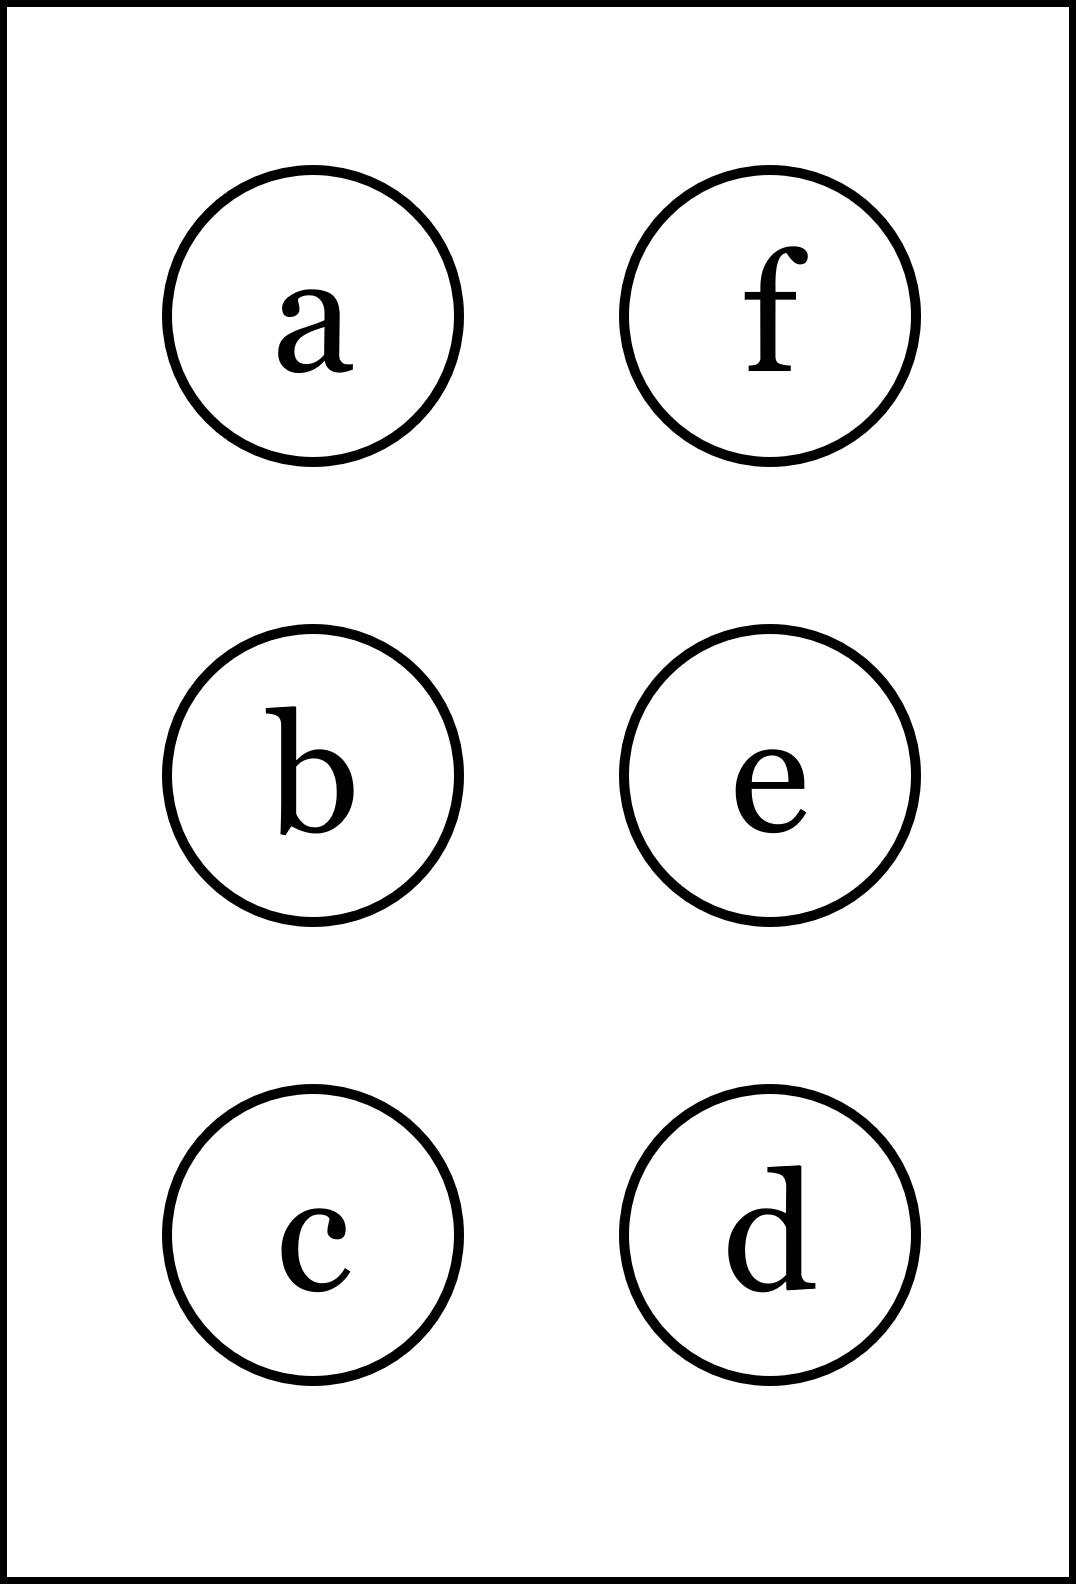
\includegraphics[height=40mm]{../images/braille.png}
{\small Písmeno Braillovej abecedy}
\end{center}
\end{minipage}
\end{center}
\end{minipage}
&
\begin{minipage}[c][104.5mm][t]{0.5\linewidth}
\begin{center}
\vspace{7mm}
{\huge Kubická rovnice, skupina \textit{Alpha $\alpha$} -\romannumeral2}\\[5mm]
\textit{Jméno:}\phantom{xxxxxxxxxxxxxxxxxxxxxxxxxxxxxxxxxxxxxxxxxxxxxxxxxxxxxxxxxxxxxxxxx}\\[5mm]
\begin{minipage}{0.95\linewidth}
\begin{center}
\textbf{Vypočítej součet kořenů kubické rovnice.} Dvojitý kořen považuj do součtu za dva,\\trojitý kořen za tři. Pokud ti vyjde stejný výsledek jako je za otazníky, tak napravo\\barvi příslušející kroužek načerno. \textbf{Spolu odevzdejte výsledné slovo}.
\end{center}
\end{minipage}
\\[1mm]
\begin{minipage}{0.79\linewidth}
\begin{center}
\begin{varwidth}{\linewidth}
\begin{enumerate}
\Large
\item $-2x^3+14x^2-20x=0$\quad \dotfill\; ???\;\dotfill \quad $7$
\item $-x^3+13x^2-47x+35=0$\quad \dotfill\; ???\;\dotfill \quad $3$
\item $9x^3+3x^2-36x-12=0$\quad \dotfill\; ???\;\dotfill \quad $\nicefrac{-1}{3}$
\item $-4x^3+14x^2+28x+10=0$\quad \dotfill\; ???\;\dotfill \quad $\nicefrac{9}{2}$
\item \quad \dotfill\; ???\;\dotfill \quad nebarvi
\item \quad \dotfill\; ???\;\dotfill \quad nebarvi
\end{enumerate}
\end{varwidth}
\end{center}
\end{minipage}
\begin{minipage}{0.20\linewidth}
\begin{center}
{\Huge\bfseries 2.} \\[2mm]
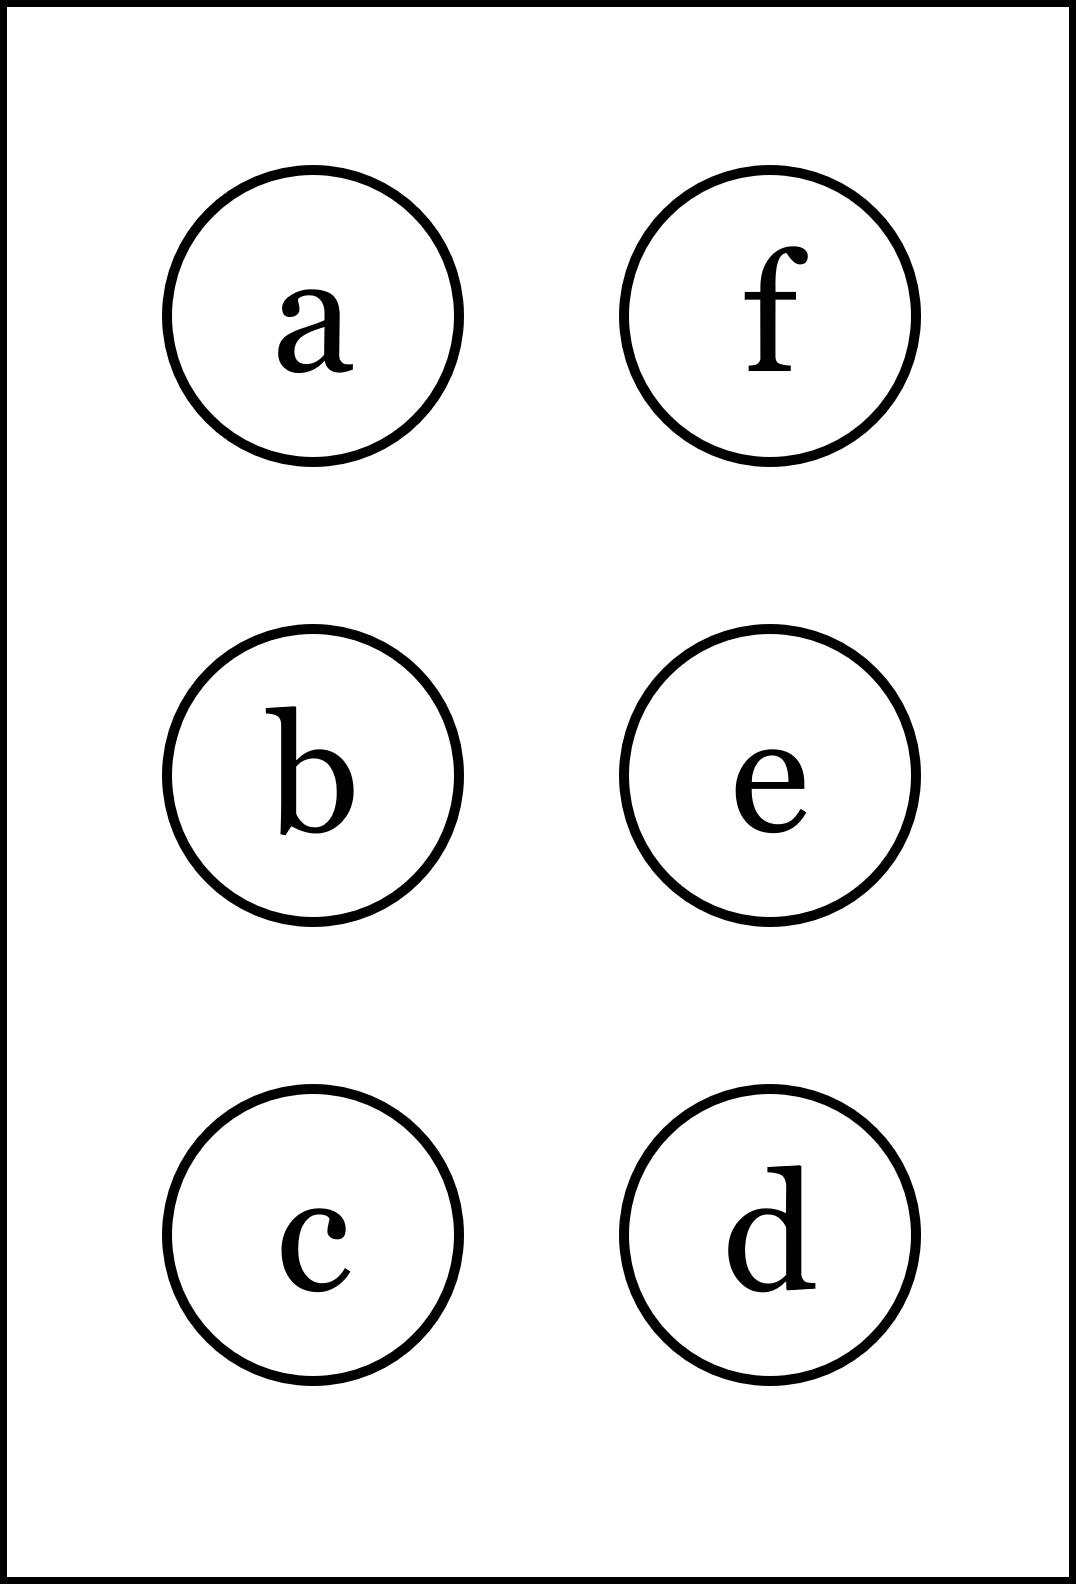
\includegraphics[height=40mm]{../images/braille.png}
{\small Písmeno Braillovej abecedy}
\end{center}
\end{minipage}
\end{center}
\end{minipage}
\\ \hdashline
\begin{minipage}[c][104.5mm][t]{0.5\linewidth}
\begin{center}
\vspace{7mm}
{\huge Kubická rovnice, skupina \textit{Alpha $\alpha$} -\romannumeral3}\\[5mm]
\textit{Jméno:}\phantom{xxxxxxxxxxxxxxxxxxxxxxxxxxxxxxxxxxxxxxxxxxxxxxxxxxxxxxxxxxxxxxxxx}\\[5mm]
\begin{minipage}{0.95\linewidth}
\begin{center}
\textbf{Vypočítej součet kořenů kubické rovnice.} Dvojitý kořen považuj do součtu za dva,\\trojitý kořen za tři. Pokud ti vyjde stejný výsledek jako je za otazníky, tak napravo\\barvi příslušející kroužek načerno. \textbf{Spolu odevzdejte výsledné slovo}.
\end{center}
\end{minipage}
\\[1mm]
\begin{minipage}{0.79\linewidth}
\begin{center}
\begin{varwidth}{\linewidth}
\begin{enumerate}
\Large
\item $-4x^3-24x^2-32x=0$\quad \dotfill\; ???\;\dotfill \quad $-6$
\item $x^3+x^2-x-1=0$\quad \dotfill\; ???\;\dotfill \quad $1$
\item $-16x^3+64x^2-80x+32=0$\quad \dotfill\; ???\;\dotfill \quad $4$
\item $-2x^3-x^2+18x+9=0$\quad \dotfill\; ???\;\dotfill \quad $\nicefrac{11}{2}$
\item \quad \dotfill\; ???\;\dotfill \quad vybarvi
\item \quad \dotfill\; ???\;\dotfill \quad vybarvi
\end{enumerate}
\end{varwidth}
\end{center}
\end{minipage}
\begin{minipage}{0.20\linewidth}
\begin{center}
{\Huge\bfseries 3.} \\[2mm]
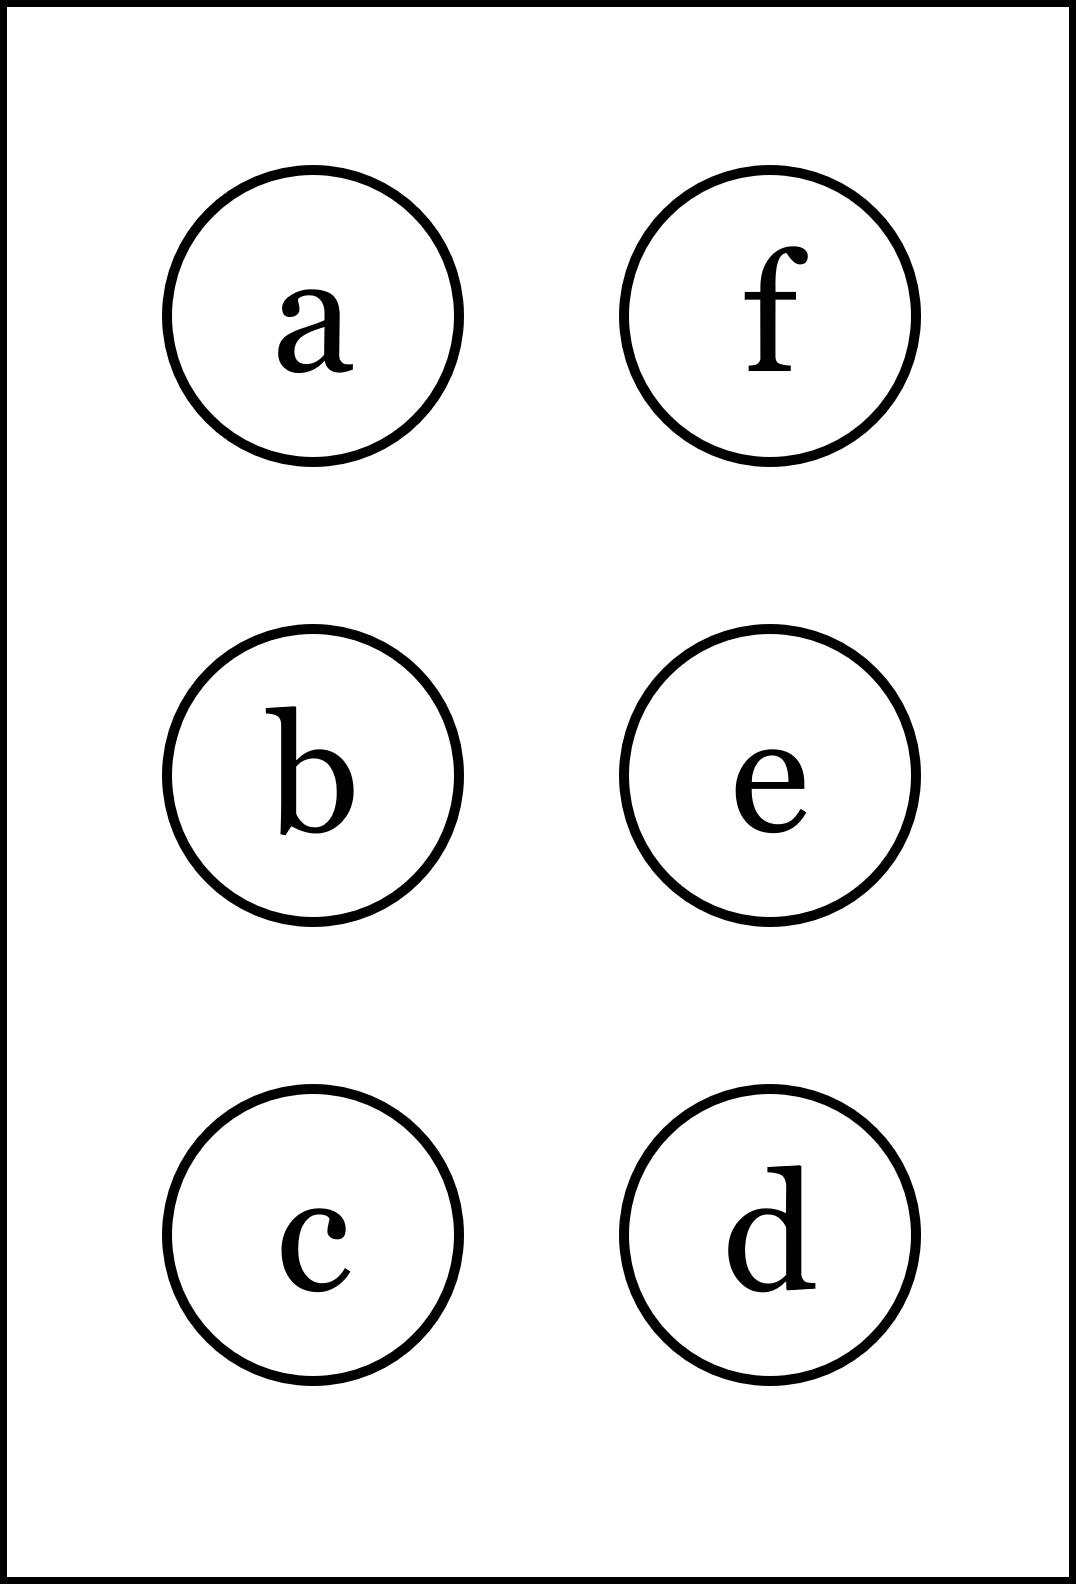
\includegraphics[height=40mm]{../images/braille.png}
{\small Písmeno Braillovej abecedy}
\end{center}
\end{minipage}
\end{center}
\end{minipage}
&
\begin{minipage}[c][104.5mm][t]{0.5\linewidth}
\begin{center}
\vspace{7mm}
{\huge Kubická rovnice, skupina \textit{Alpha $\alpha$} -\romannumeral4}\\[5mm]
\textit{Jméno:}\phantom{xxxxxxxxxxxxxxxxxxxxxxxxxxxxxxxxxxxxxxxxxxxxxxxxxxxxxxxxxxxxxxxxx}\\[5mm]
\begin{minipage}{0.95\linewidth}
\begin{center}
\textbf{Vypočítej součet kořenů kubické rovnice.} Dvojitý kořen považuj do součtu za dva,\\trojitý kořen za tři. Pokud ti vyjde stejný výsledek jako je za otazníky, tak napravo\\barvi příslušející kroužek načerno. \textbf{Spolu odevzdejte výsledné slovo}.
\end{center}
\end{minipage}
\\[1mm]
\begin{minipage}{0.79\linewidth}
\begin{center}
\begin{varwidth}{\linewidth}
\begin{enumerate}
\Large
\item $x^3+6x^2+8x=0$\quad \dotfill\; ???\;\dotfill \quad $-6$
\item $-2x^3+4x^2+14x+8=0$\quad \dotfill\; ???\;\dotfill \quad $-6$
\item $25x^3+5x^2-25x-5=0$\quad \dotfill\; ???\;\dotfill \quad $\nicefrac{-1}{5}$
\item $-x^3-6x^2+19x+24=0$\quad \dotfill\; ???\;\dotfill \quad $-4$
\item \quad \dotfill\; ???\;\dotfill \quad vybarvi
\item \quad \dotfill\; ???\;\dotfill \quad nebarvi
\end{enumerate}
\end{varwidth}
\end{center}
\end{minipage}
\begin{minipage}{0.20\linewidth}
\begin{center}
{\Huge\bfseries 4.} \\[2mm]
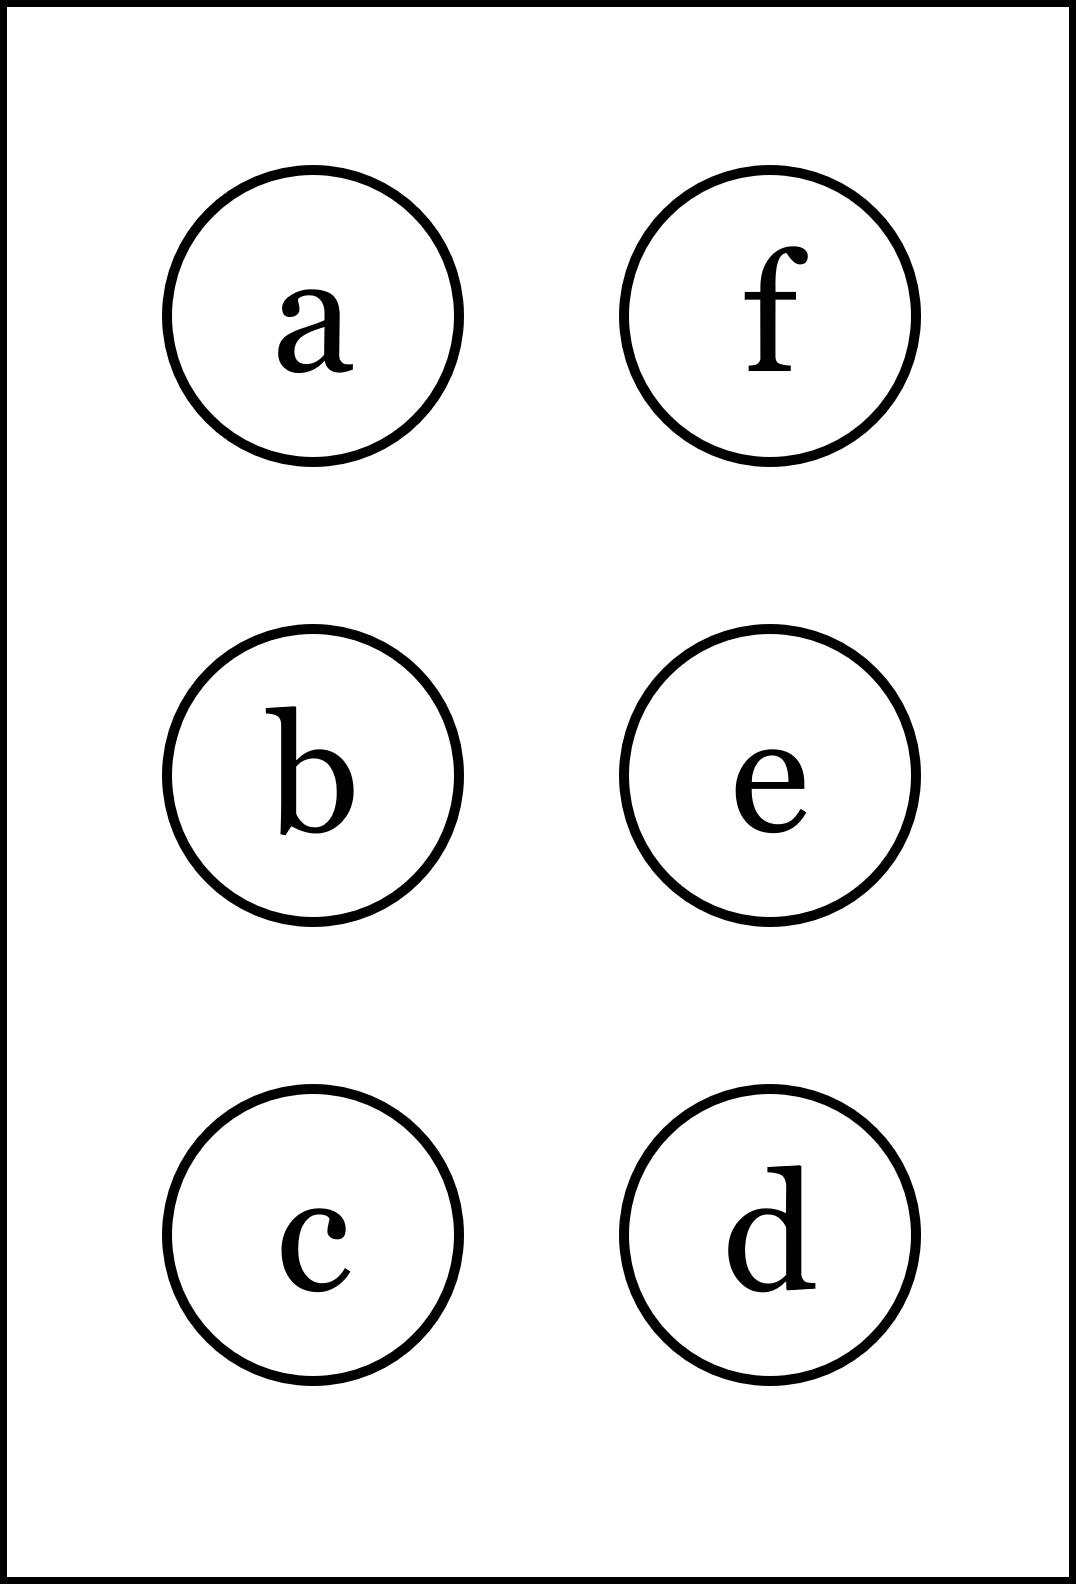
\includegraphics[height=40mm]{../images/braille.png}
{\small Písmeno Braillovej abecedy}
\end{center}
\end{minipage}
\end{center}
\end{minipage}
%
\end{tabular}
\newpage
\thispagestyle{empty}
\begin{tabular}{c:c}
\begin{minipage}[c][104.5mm][t]{0.5\linewidth}
\begin{center}
\vspace{7mm}
{\huge Kubická rovnice, skupina \textit{Beta $\beta$} -\romannumeral1}\\[5mm]
\textit{Jméno:}\phantom{xxxxxxxxxxxxxxxxxxxxxxxxxxxxxxxxxxxxxxxxxxxxxxxxxxxxxxxxxxxxxxxxx}\\[5mm]
\begin{minipage}{0.95\linewidth}
\begin{center}
\textbf{Vypočítej součet kořenů kubické rovnice.} Dvojitý kořen považuj do součtu za dva,\\trojitý kořen za tři. Pokud ti vyjde stejný výsledek jako je za otazníky, tak napravo\\barvi příslušející kroužek načerno. \textbf{Spolu odevzdejte výsledné slovo}.
\end{center}
\end{minipage}
\\[1mm]
\begin{minipage}{0.79\linewidth}
\begin{center}
\begin{varwidth}{\linewidth}
\begin{enumerate}
\Large
\item $-x^3-4x^2-4x=0$\quad \dotfill\; ???\;\dotfill \quad $-4$
\item $2x^3+14x^2-20x-32=0$\quad \dotfill\; ???\;\dotfill \quad $9$
\item $-5x^3+20x^2-5x-30=0$\quad \dotfill\; ???\;\dotfill \quad $0$
\item $-10x^3-12x^2+18x+4=0$\quad \dotfill\; ???\;\dotfill \quad $\nicefrac{-6}{5}$
\item \quad \dotfill\; ???\;\dotfill \quad nebarvi
\item \quad \dotfill\; ???\;\dotfill \quad vybarvi
\end{enumerate}
\end{varwidth}
\end{center}
\end{minipage}
\begin{minipage}{0.20\linewidth}
\begin{center}
{\Huge\bfseries 1.} \\[2mm]
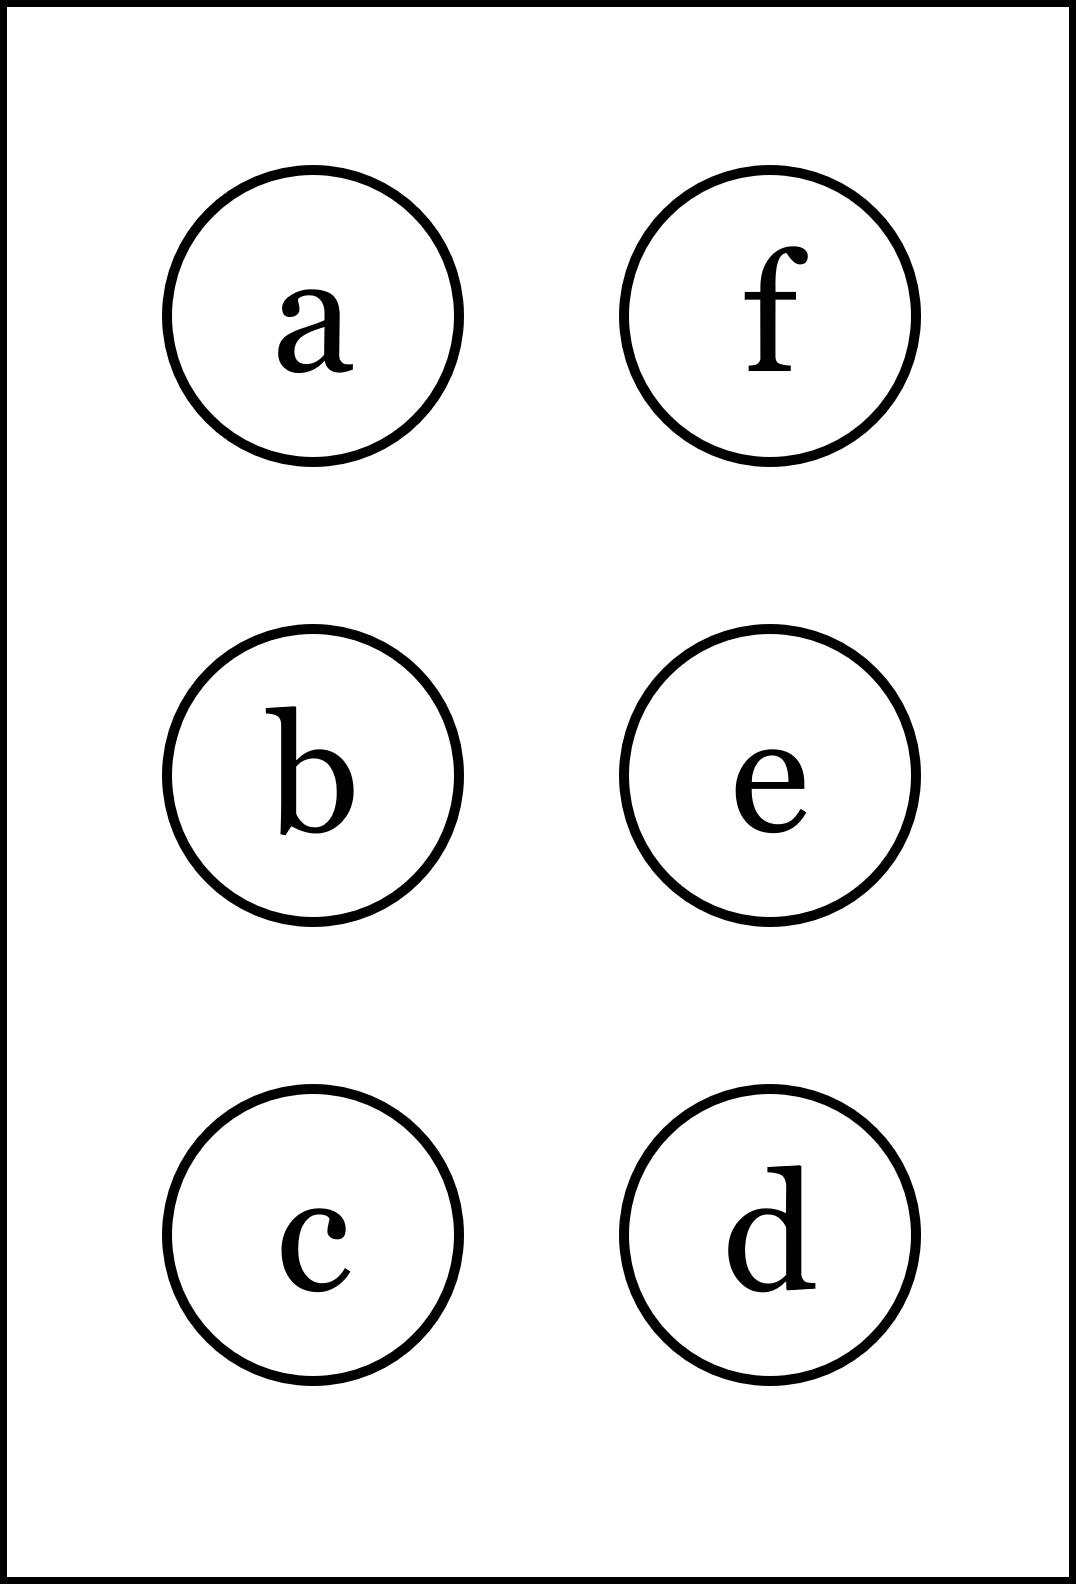
\includegraphics[height=40mm]{../images/braille.png}
{\small Písmeno Braillovej abecedy}
\end{center}
\end{minipage}
\end{center}
\end{minipage}
&
\begin{minipage}[c][104.5mm][t]{0.5\linewidth}
\begin{center}
\vspace{7mm}
{\huge Kubická rovnice, skupina \textit{Beta $\beta$} -\romannumeral2}\\[5mm]
\textit{Jméno:}\phantom{xxxxxxxxxxxxxxxxxxxxxxxxxxxxxxxxxxxxxxxxxxxxxxxxxxxxxxxxxxxxxxxxx}\\[5mm]
\begin{minipage}{0.95\linewidth}
\begin{center}
\textbf{Vypočítej součet kořenů kubické rovnice.} Dvojitý kořen považuj do součtu za dva,\\trojitý kořen za tři. Pokud ti vyjde stejný výsledek jako je za otazníky, tak napravo\\barvi příslušející kroužek načerno. \textbf{Spolu odevzdejte výsledné slovo}.
\end{center}
\end{minipage}
\\[1mm]
\begin{minipage}{0.79\linewidth}
\begin{center}
\begin{varwidth}{\linewidth}
\begin{enumerate}
\Large
\item $2x^3+8x^2-24x=0$\quad \dotfill\; ???\;\dotfill \quad $-4$
\item $x^3+7x^2+4x-12=0$\quad \dotfill\; ???\;\dotfill \quad $-3$
\item $-8x^3-56x^2+8x+56=0$\quad \dotfill\; ???\;\dotfill \quad $7$
\item $-4x^3+6x^2+40x-42=0$\quad \dotfill\; ???\;\dotfill \quad $\nicefrac{15}{2}$
\item \quad \dotfill\; ???\;\dotfill \quad vybarvi
\item \quad \dotfill\; ???\;\dotfill \quad nebarvi
\end{enumerate}
\end{varwidth}
\end{center}
\end{minipage}
\begin{minipage}{0.20\linewidth}
\begin{center}
{\Huge\bfseries 2.} \\[2mm]
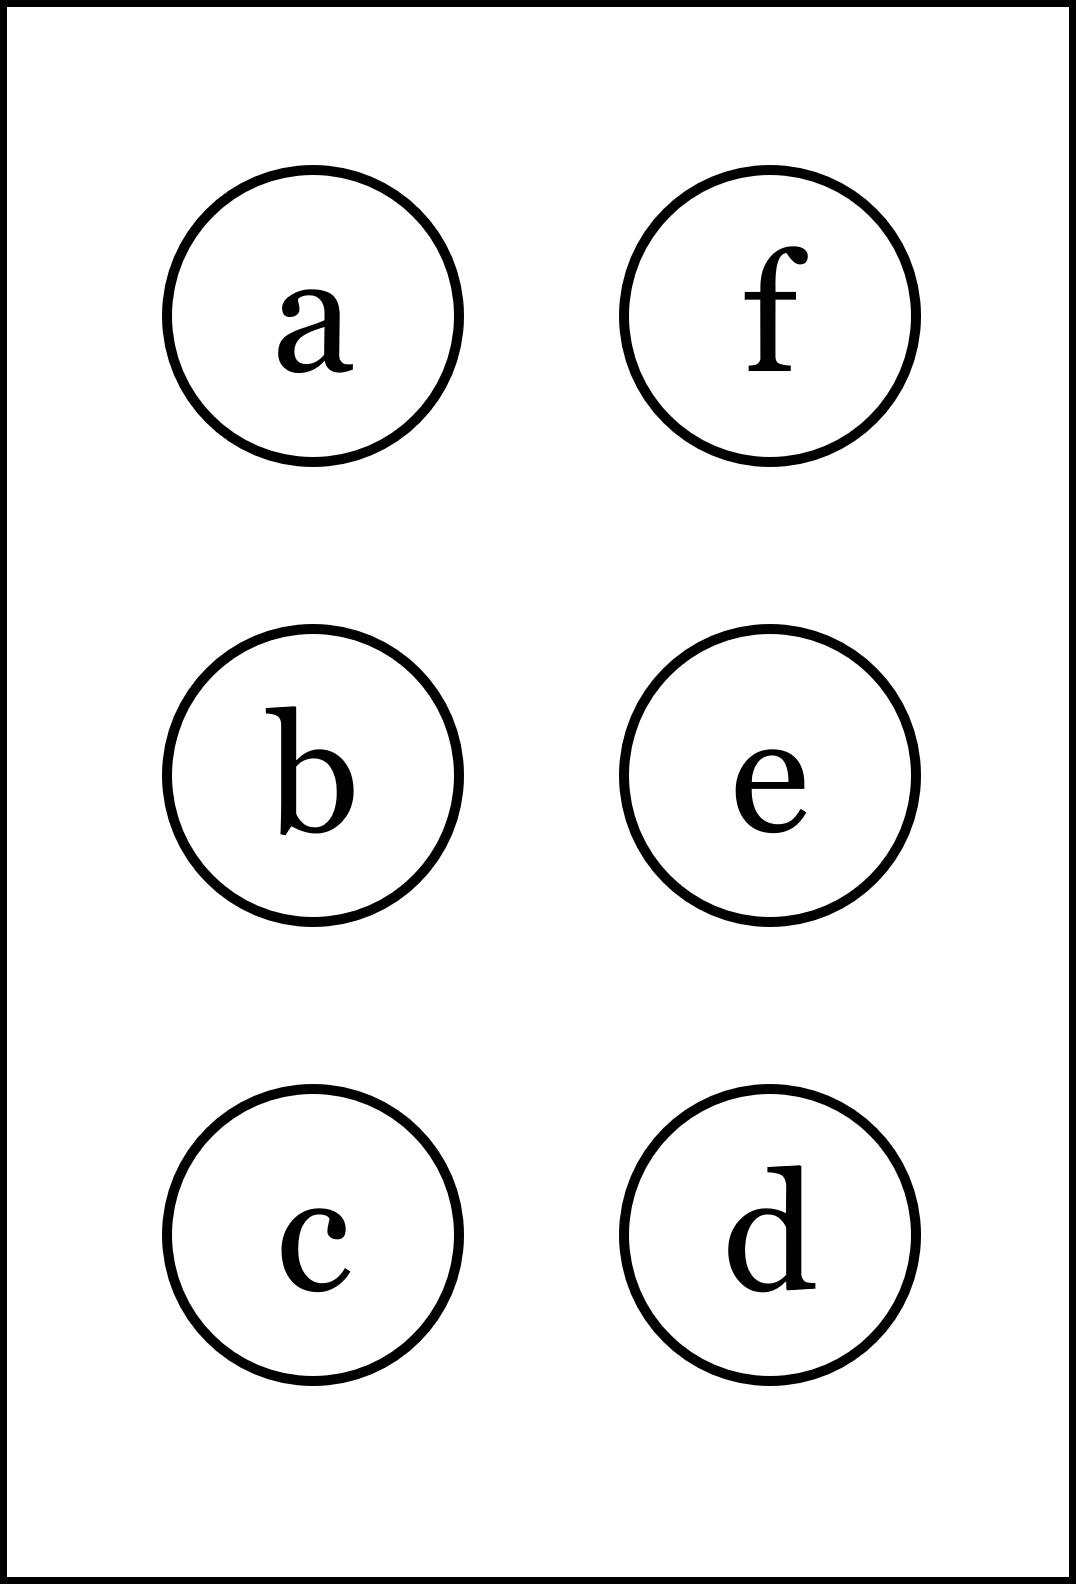
\includegraphics[height=40mm]{../images/braille.png}
{\small Písmeno Braillovej abecedy}
\end{center}
\end{minipage}
\end{center}
\end{minipage}
\\ \hdashline
\begin{minipage}[c][104.5mm][t]{0.5\linewidth}
\begin{center}
\vspace{7mm}
{\huge Kubická rovnice, skupina \textit{Beta $\beta$} -\romannumeral3}\\[5mm]
\textit{Jméno:}\phantom{xxxxxxxxxxxxxxxxxxxxxxxxxxxxxxxxxxxxxxxxxxxxxxxxxxxxxxxxxxxxxxxxx}\\[5mm]
\begin{minipage}{0.95\linewidth}
\begin{center}
\textbf{Vypočítej součet kořenů kubické rovnice.} Dvojitý kořen považuj do součtu za dva,\\trojitý kořen za tři. Pokud ti vyjde stejný výsledek jako je za otazníky, tak napravo\\barvi příslušející kroužek načerno. \textbf{Spolu odevzdejte výsledné slovo}.
\end{center}
\end{minipage}
\\[1mm]
\begin{minipage}{0.79\linewidth}
\begin{center}
\begin{varwidth}{\linewidth}
\begin{enumerate}
\Large
\item $x^3+11x^2+18x=0$\quad \dotfill\; ???\;\dotfill \quad $7$
\item $x^3-4x^2-x+4=0$\quad \dotfill\; ???\;\dotfill \quad $4$
\item $-4x^3-32x^2-52x-24=0$\quad \dotfill\; ???\;\dotfill \quad $-8$
\item $-3x^3+19x^2-4x-12=0$\quad \dotfill\; ???\;\dotfill \quad $\nicefrac{23}{3}$
\item \quad \dotfill\; ???\;\dotfill \quad nebarvi
\item \quad \dotfill\; ???\;\dotfill \quad vybarvi
\end{enumerate}
\end{varwidth}
\end{center}
\end{minipage}
\begin{minipage}{0.20\linewidth}
\begin{center}
{\Huge\bfseries 3.} \\[2mm]
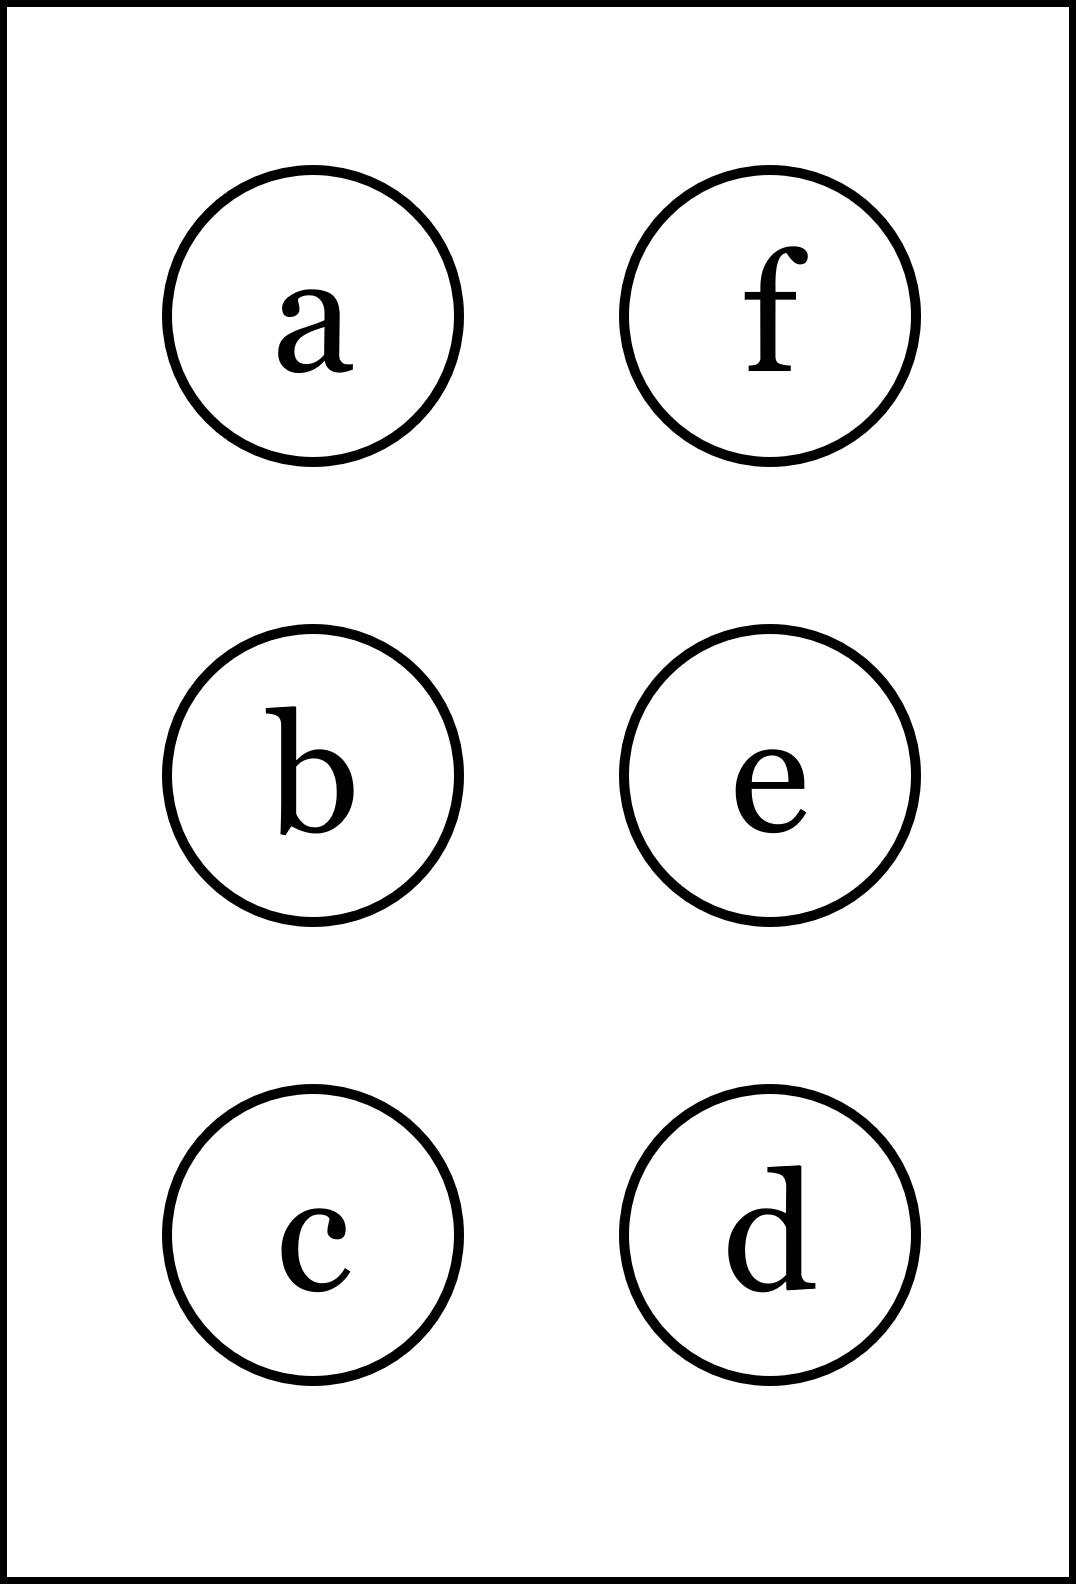
\includegraphics[height=40mm]{../images/braille.png}
{\small Písmeno Braillovej abecedy}
\end{center}
\end{minipage}
\end{center}
\end{minipage}
&
\begin{minipage}[c][104.5mm][t]{0.5\linewidth}
\begin{center}
\vspace{7mm}
{\huge Kubická rovnice, skupina \textit{Beta $\beta$} -\romannumeral4}\\[5mm]
\textit{Jméno:}\phantom{xxxxxxxxxxxxxxxxxxxxxxxxxxxxxxxxxxxxxxxxxxxxxxxxxxxxxxxxxxxxxxxxx}\\[5mm]
\begin{minipage}{0.95\linewidth}
\begin{center}
\textbf{Vypočítej součet kořenů kubické rovnice.} Dvojitý kořen považuj do součtu za dva,\\trojitý kořen za tři. Pokud ti vyjde stejný výsledek jako je za otazníky, tak napravo\\barvi příslušející kroužek načerno. \textbf{Spolu odevzdejte výsledné slovo}.
\end{center}
\end{minipage}
\\[1mm]
\begin{minipage}{0.79\linewidth}
\begin{center}
\begin{varwidth}{\linewidth}
\begin{enumerate}
\Large
\item $-x^3-x^2+2x=0$\quad \dotfill\; ???\;\dotfill \quad $-3$
\item $-x^3+13x+12=0$\quad \dotfill\; ???\;\dotfill \quad $0$
\item $12x^3+24x^2-12x-24=0$\quad \dotfill\; ???\;\dotfill \quad $-2$
\item $-35x^3-37x^2-x+1=0$\quad \dotfill\; ???\;\dotfill \quad $\nicefrac{-23}{35}$
\item \quad \dotfill\; ???\;\dotfill \quad vybarvi
\item \quad \dotfill\; ???\;\dotfill \quad vybarvi
\end{enumerate}
\end{varwidth}
\end{center}
\end{minipage}
\begin{minipage}{0.20\linewidth}
\begin{center}
{\Huge\bfseries 4.} \\[2mm]
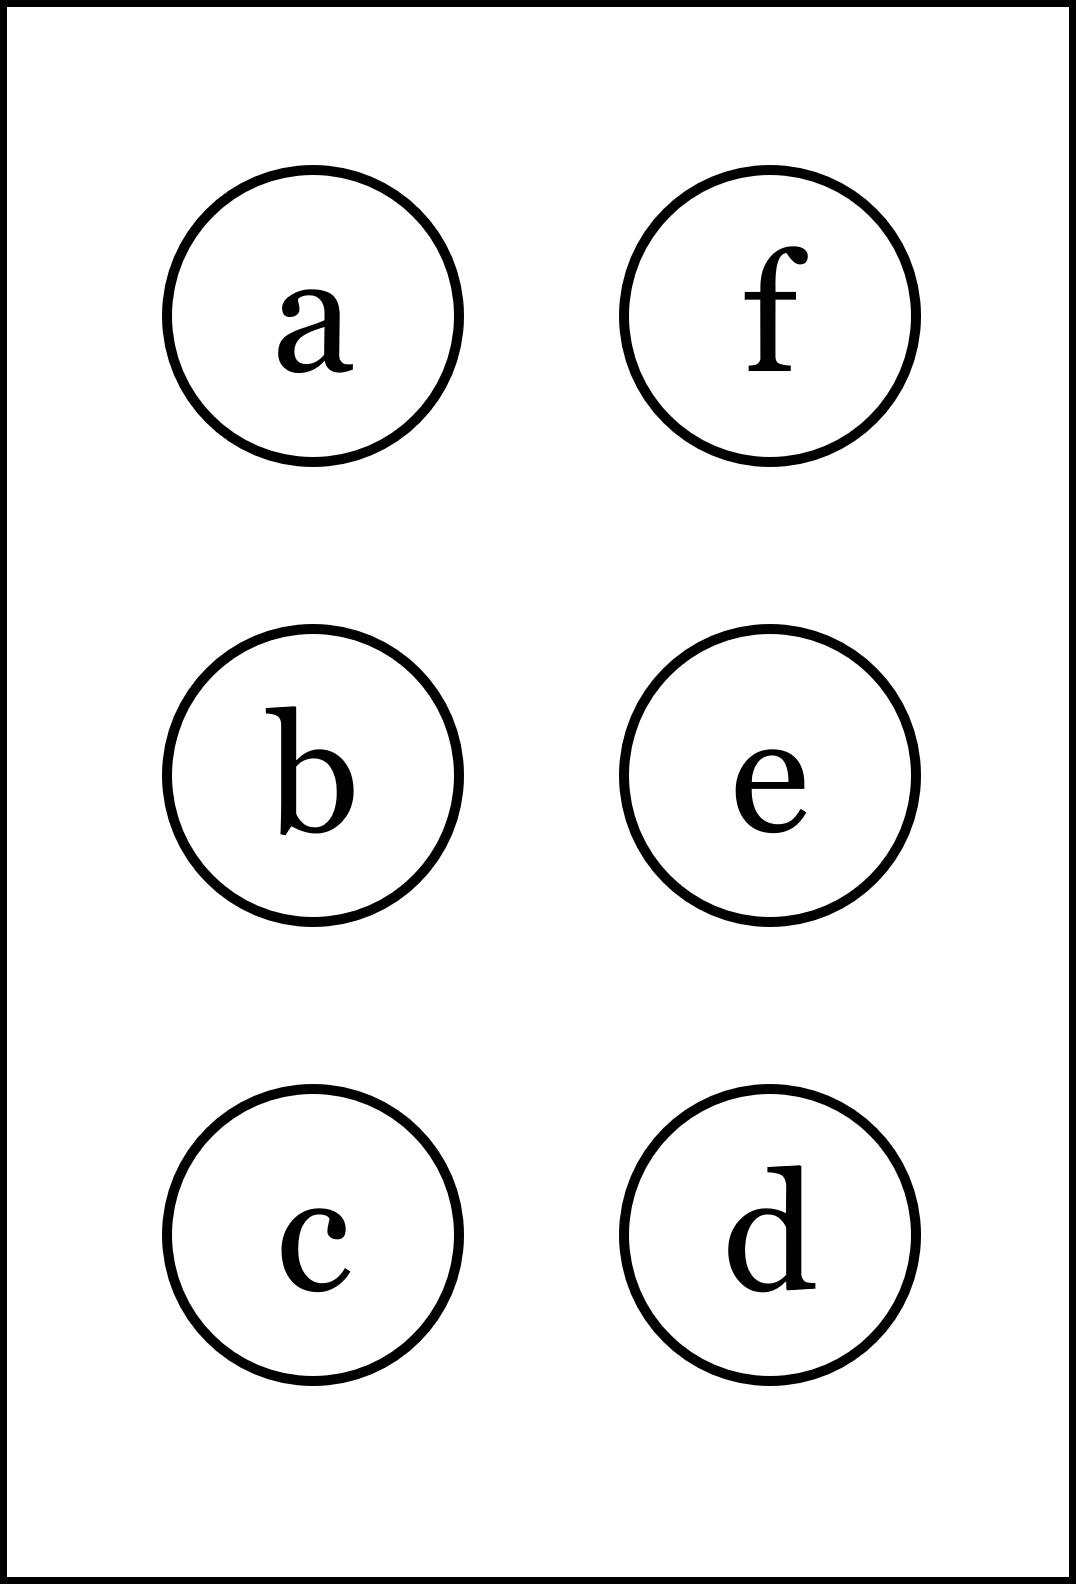
\includegraphics[height=40mm]{../images/braille.png}
{\small Písmeno Braillovej abecedy}
\end{center}
\end{minipage}
\end{center}
\end{minipage}
%
\end{tabular}
\newpage
\thispagestyle{empty}
\begin{tabular}{c:c}
\begin{minipage}[c][104.5mm][t]{0.5\linewidth}
\begin{center}
\vspace{7mm}
{\huge Kubická rovnice, skupina \textit{Gamma $\gamma$} -\romannumeral1}\\[5mm]
\textit{Jméno:}\phantom{xxxxxxxxxxxxxxxxxxxxxxxxxxxxxxxxxxxxxxxxxxxxxxxxxxxxxxxxxxxxxxxxx}\\[5mm]
\begin{minipage}{0.95\linewidth}
\begin{center}
\textbf{Vypočítej součet kořenů kubické rovnice.} Dvojitý kořen považuj do součtu za dva,\\trojitý kořen za tři. Pokud ti vyjde stejný výsledek jako je za otazníky, tak napravo\\barvi příslušející kroužek načerno. \textbf{Spolu odevzdejte výsledné slovo}.
\end{center}
\end{minipage}
\\[1mm]
\begin{minipage}{0.79\linewidth}
\begin{center}
\begin{varwidth}{\linewidth}
\begin{enumerate}
\Large
\item $4x^3+16x^2+12x=0$\quad \dotfill\; ???\;\dotfill \quad $-4$
\item $x^3+x^2-8x-12=0$\quad \dotfill\; ???\;\dotfill \quad $3$
\item $3x^3+9x^2-12x-36=0$\quad \dotfill\; ???\;\dotfill \quad $-3$
\item $-20x^3-52x^2-44x-12=0$\quad \dotfill\; ???\;\dotfill \quad $\nicefrac{-7}{5}$
\item \quad \dotfill\; ???\;\dotfill \quad vybarvi
\item \quad \dotfill\; ???\;\dotfill \quad nebarvi
\end{enumerate}
\end{varwidth}
\end{center}
\end{minipage}
\begin{minipage}{0.20\linewidth}
\begin{center}
{\Huge\bfseries 1.} \\[2mm]
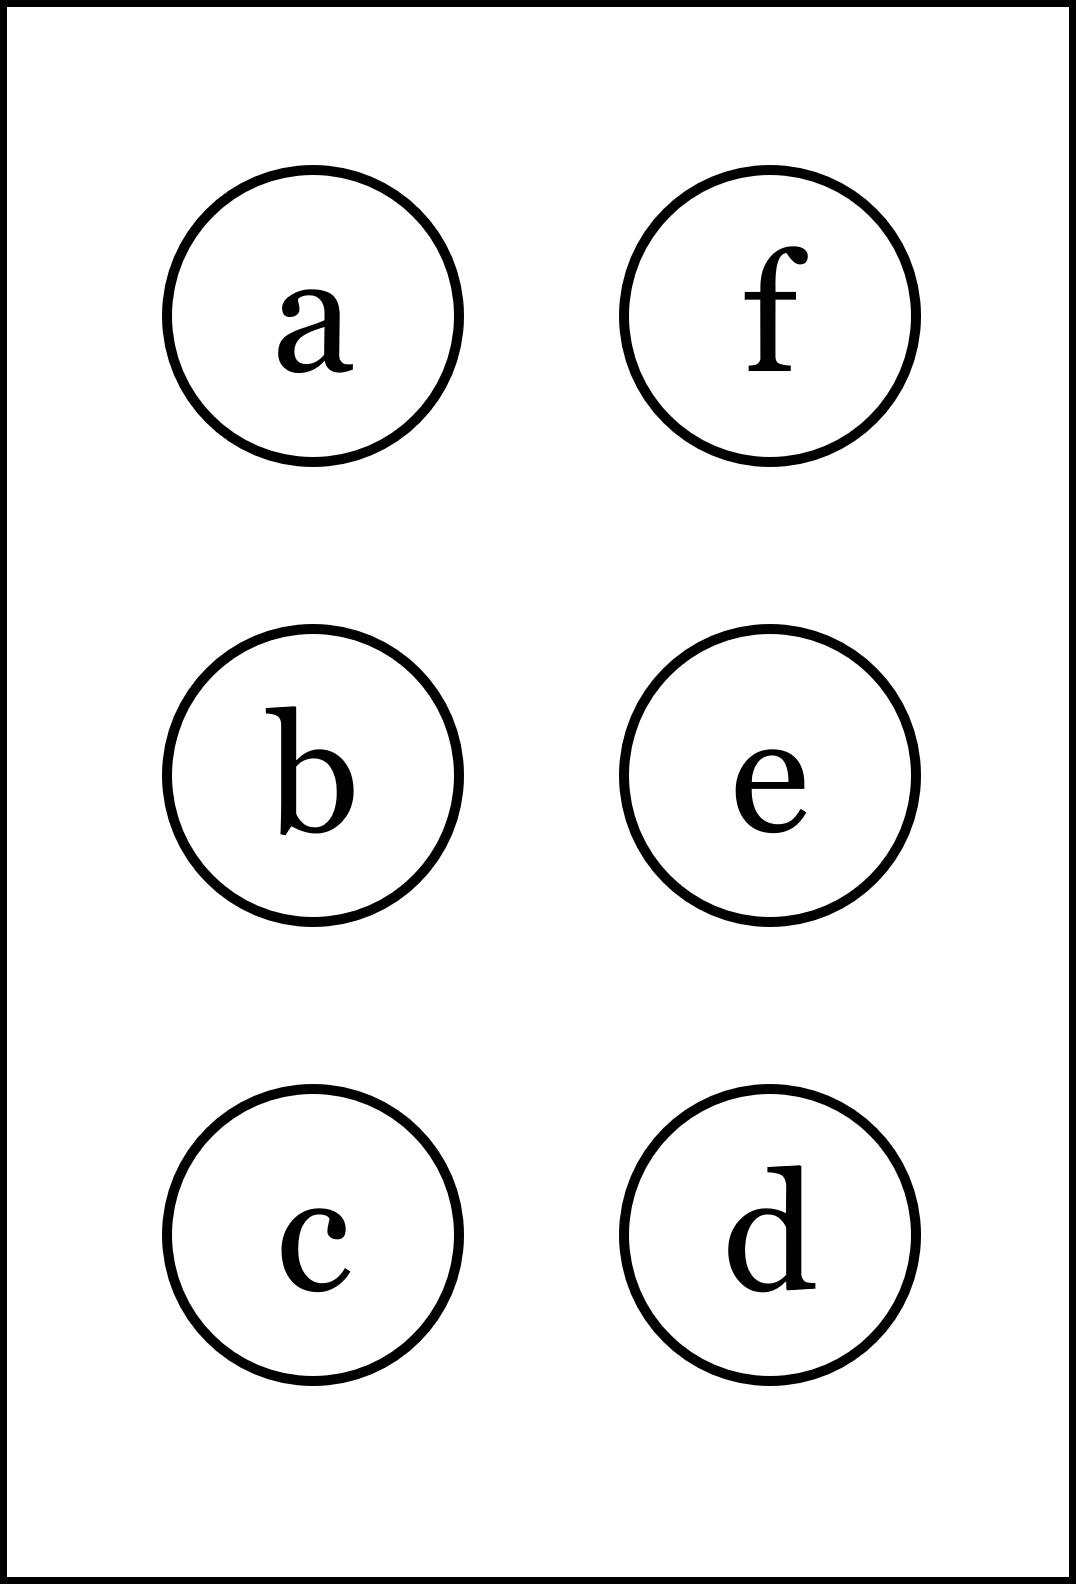
\includegraphics[height=40mm]{../images/braille.png}
{\small Písmeno Braillovej abecedy}
\end{center}
\end{minipage}
\end{center}
\end{minipage}
&
\begin{minipage}[c][104.5mm][t]{0.5\linewidth}
\begin{center}
\vspace{7mm}
{\huge Kubická rovnice, skupina \textit{Gamma $\gamma$} -\romannumeral2}\\[5mm]
\textit{Jméno:}\phantom{xxxxxxxxxxxxxxxxxxxxxxxxxxxxxxxxxxxxxxxxxxxxxxxxxxxxxxxxxxxxxxxxx}\\[5mm]
\begin{minipage}{0.95\linewidth}
\begin{center}
\textbf{Vypočítej součet kořenů kubické rovnice.} Dvojitý kořen považuj do součtu za dva,\\trojitý kořen za tři. Pokud ti vyjde stejný výsledek jako je za otazníky, tak napravo\\barvi příslušející kroužek načerno. \textbf{Spolu odevzdejte výsledné slovo}.
\end{center}
\end{minipage}
\\[1mm]
\begin{minipage}{0.79\linewidth}
\begin{center}
\begin{varwidth}{\linewidth}
\begin{enumerate}
\Large
\item $-x^3-3x^2+4x=0$\quad \dotfill\; ???\;\dotfill \quad $-5$
\item $-x^3+4x^2+25x-28=0$\quad \dotfill\; ???\;\dotfill \quad $4$
\item $-14x^3-68x^2-90x-36=0$\quad \dotfill\; ???\;\dotfill \quad $\nicefrac{-34}{7}$
\item $15x^3+33x^2-6x-24=0$\quad \dotfill\; ???\;\dotfill \quad $\nicefrac{-19}{5}$
\item \quad \dotfill\; ???\;\dotfill \quad nebarvi
\item \quad \dotfill\; ???\;\dotfill \quad vybarvi
\end{enumerate}
\end{varwidth}
\end{center}
\end{minipage}
\begin{minipage}{0.20\linewidth}
\begin{center}
{\Huge\bfseries 2.} \\[2mm]
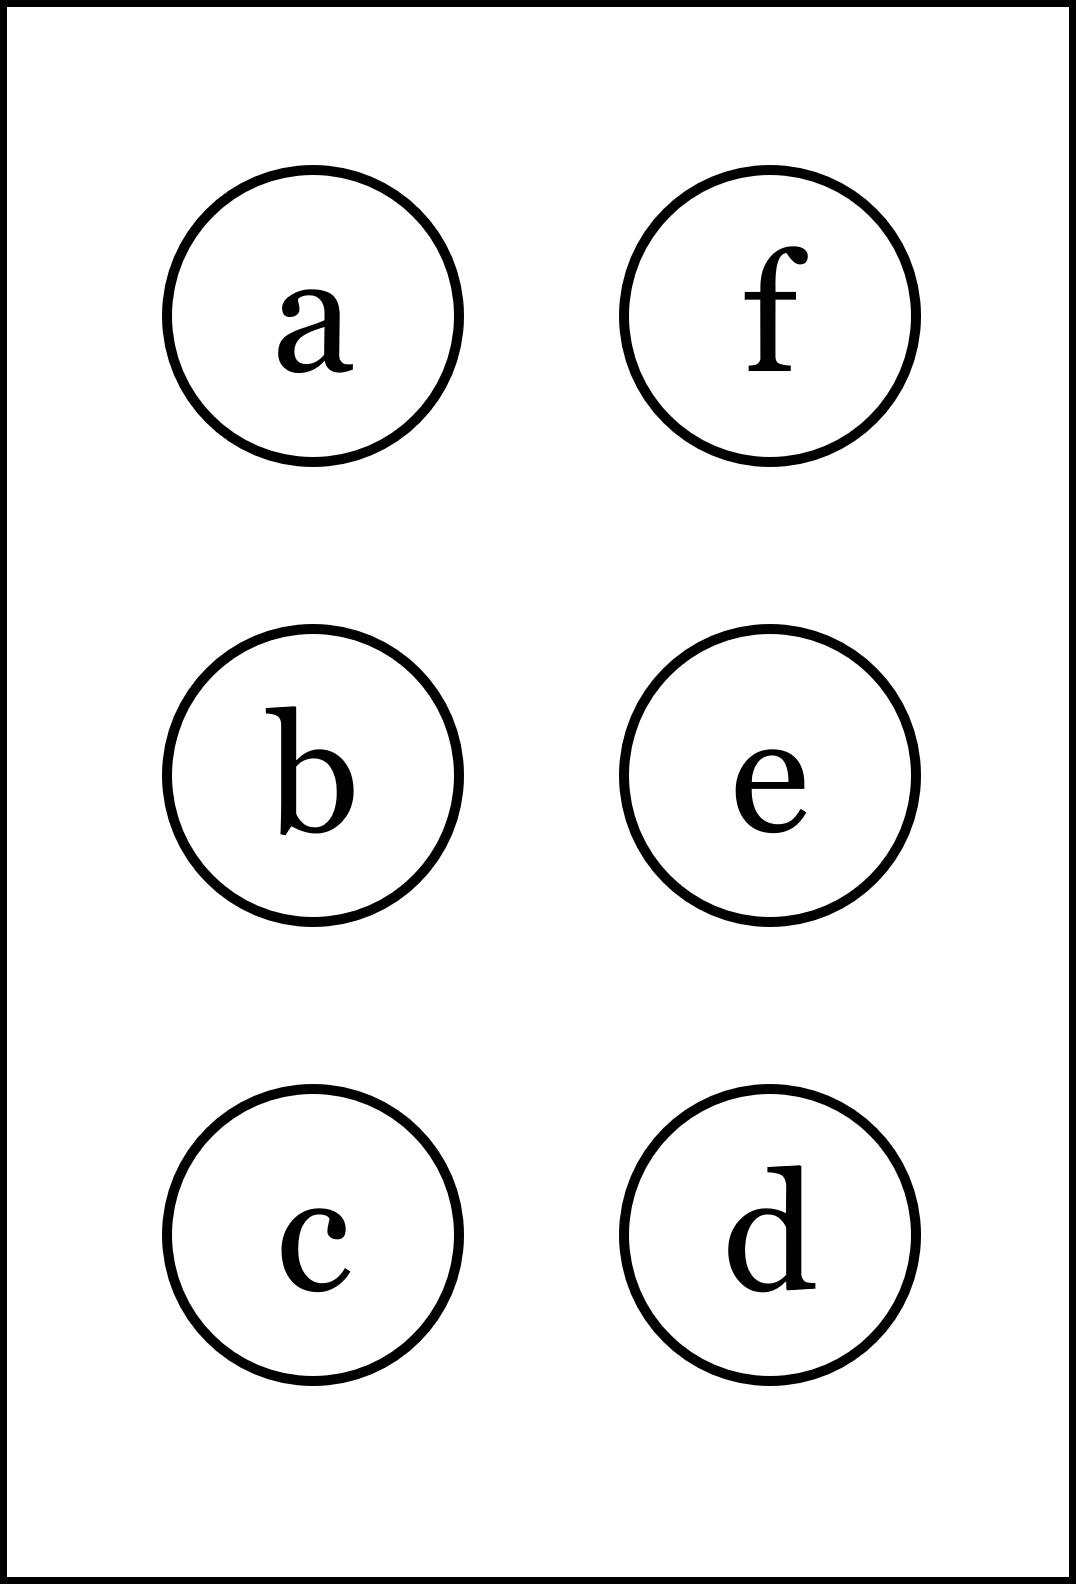
\includegraphics[height=40mm]{../images/braille.png}
{\small Písmeno Braillovej abecedy}
\end{center}
\end{minipage}
\end{center}
\end{minipage}
\\ \hdashline
\begin{minipage}[c][104.5mm][t]{0.5\linewidth}
\begin{center}
\vspace{7mm}
{\huge Kubická rovnice, skupina \textit{Gamma $\gamma$} -\romannumeral3}\\[5mm]
\textit{Jméno:}\phantom{xxxxxxxxxxxxxxxxxxxxxxxxxxxxxxxxxxxxxxxxxxxxxxxxxxxxxxxxxxxxxxxxx}\\[5mm]
\begin{minipage}{0.95\linewidth}
\begin{center}
\textbf{Vypočítej součet kořenů kubické rovnice.} Dvojitý kořen považuj do součtu za dva,\\trojitý kořen za tři. Pokud ti vyjde stejný výsledek jako je za otazníky, tak napravo\\barvi příslušející kroužek načerno. \textbf{Spolu odevzdejte výsledné slovo}.
\end{center}
\end{minipage}
\\[1mm]
\begin{minipage}{0.79\linewidth}
\begin{center}
\begin{varwidth}{\linewidth}
\begin{enumerate}
\Large
\item $4x^3+12x^2+8x=0$\quad \dotfill\; ???\;\dotfill \quad $-3$
\item $3x^3-3x^2-27x+27=0$\quad \dotfill\; ???\;\dotfill \quad $7$
\item $6x^3-30x^2+42x-18=0$\quad \dotfill\; ???\;\dotfill \quad $3$
\item $21x^3+44x^2+x-6=0$\quad \dotfill\; ???\;\dotfill \quad $\nicefrac{-26}{21}$
\item \quad \dotfill\; ???\;\dotfill \quad vybarvi
\item \quad \dotfill\; ???\;\dotfill \quad nebarvi
\end{enumerate}
\end{varwidth}
\end{center}
\end{minipage}
\begin{minipage}{0.20\linewidth}
\begin{center}
{\Huge\bfseries 3.} \\[2mm]
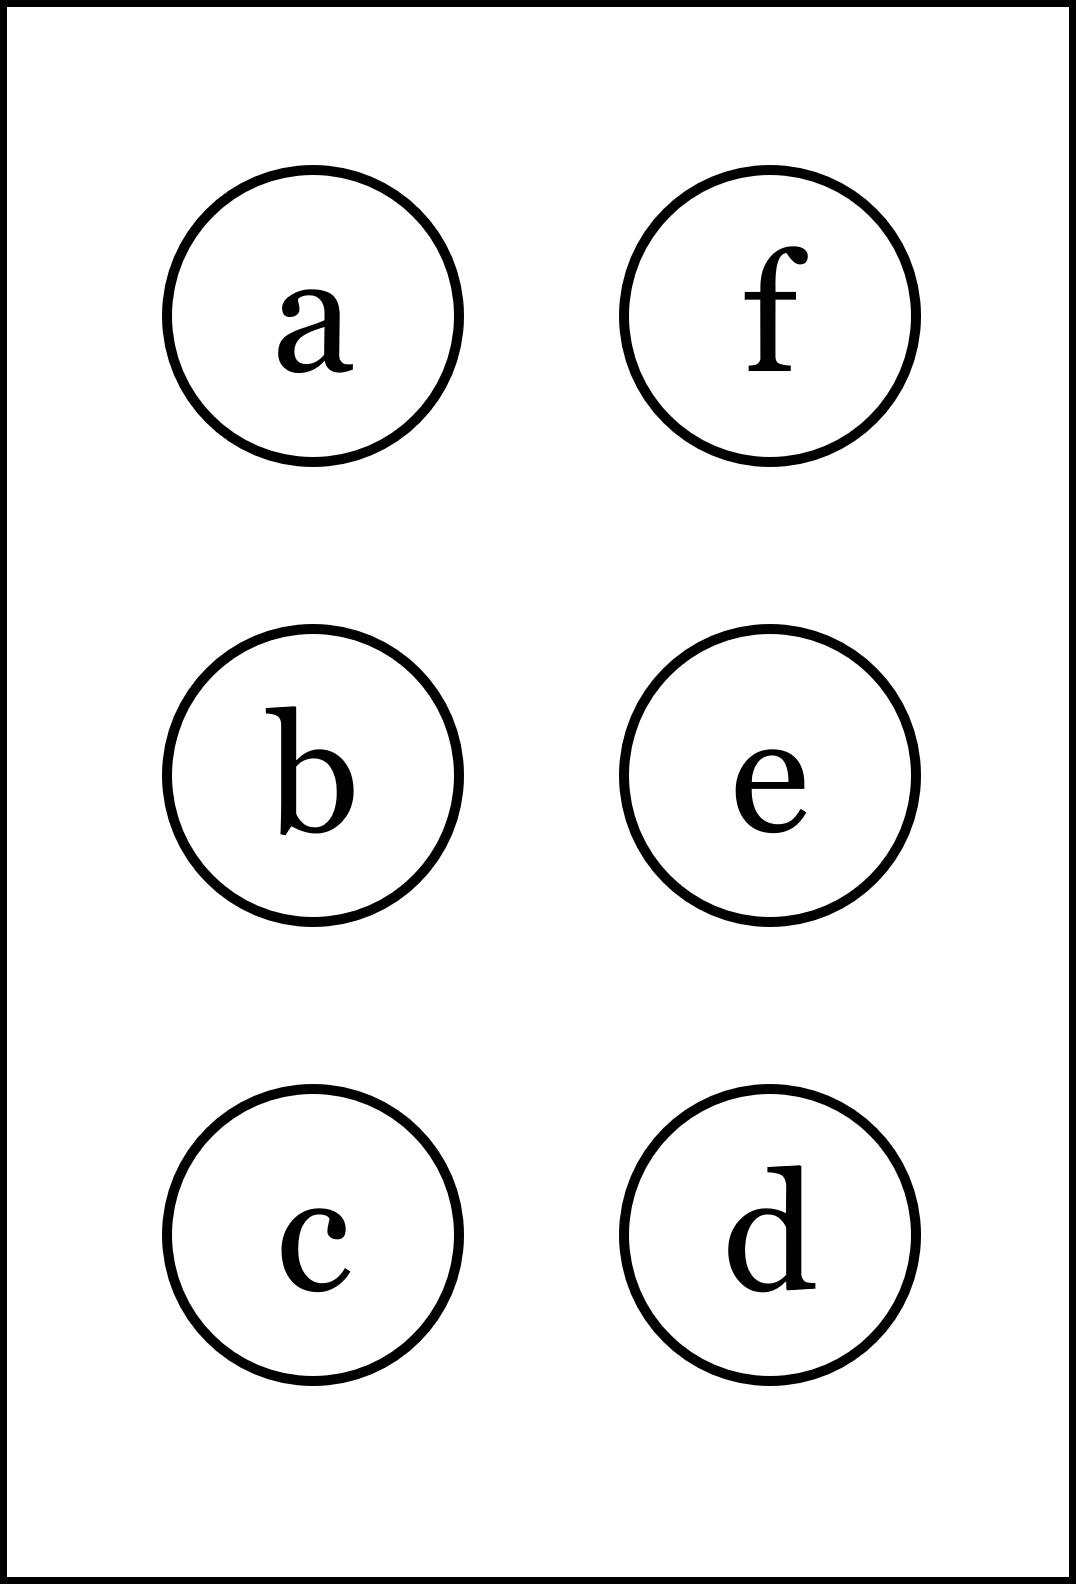
\includegraphics[height=40mm]{../images/braille.png}
{\small Písmeno Braillovej abecedy}
\end{center}
\end{minipage}
\end{center}
\end{minipage}
&
\begin{minipage}[c][104.5mm][t]{0.5\linewidth}
\begin{center}
\vspace{7mm}
{\huge Kubická rovnice, skupina \textit{Gamma $\gamma$} -\romannumeral4}\\[5mm]
\textit{Jméno:}\phantom{xxxxxxxxxxxxxxxxxxxxxxxxxxxxxxxxxxxxxxxxxxxxxxxxxxxxxxxxxxxxxxxxx}\\[5mm]
\begin{minipage}{0.95\linewidth}
\begin{center}
\textbf{Vypočítej součet kořenů kubické rovnice.} Dvojitý kořen považuj do součtu za dva,\\trojitý kořen za tři. Pokud ti vyjde stejný výsledek jako je za otazníky, tak napravo\\barvi příslušející kroužek načerno. \textbf{Spolu odevzdejte výsledné slovo}.
\end{center}
\end{minipage}
\\[1mm]
\begin{minipage}{0.79\linewidth}
\begin{center}
\begin{varwidth}{\linewidth}
\begin{enumerate}
\Large
\item $x^3-7x^2-8x=0$\quad \dotfill\; ???\;\dotfill \quad $7$
\item $-x^3+2x^2+7x+4=0$\quad \dotfill\; ???\;\dotfill \quad $2$
\item $-2x^3-8x^2+2x+8=0$\quad \dotfill\; ???\;\dotfill \quad $-4$
\item $18x^3-69x^2+78x-24=0$\quad \dotfill\; ???\;\dotfill \quad $\nicefrac{17}{6}$
\item \quad \dotfill\; ???\;\dotfill \quad nebarvi
\item \quad \dotfill\; ???\;\dotfill \quad nebarvi
\end{enumerate}
\end{varwidth}
\end{center}
\end{minipage}
\begin{minipage}{0.20\linewidth}
\begin{center}
{\Huge\bfseries 4.} \\[2mm]
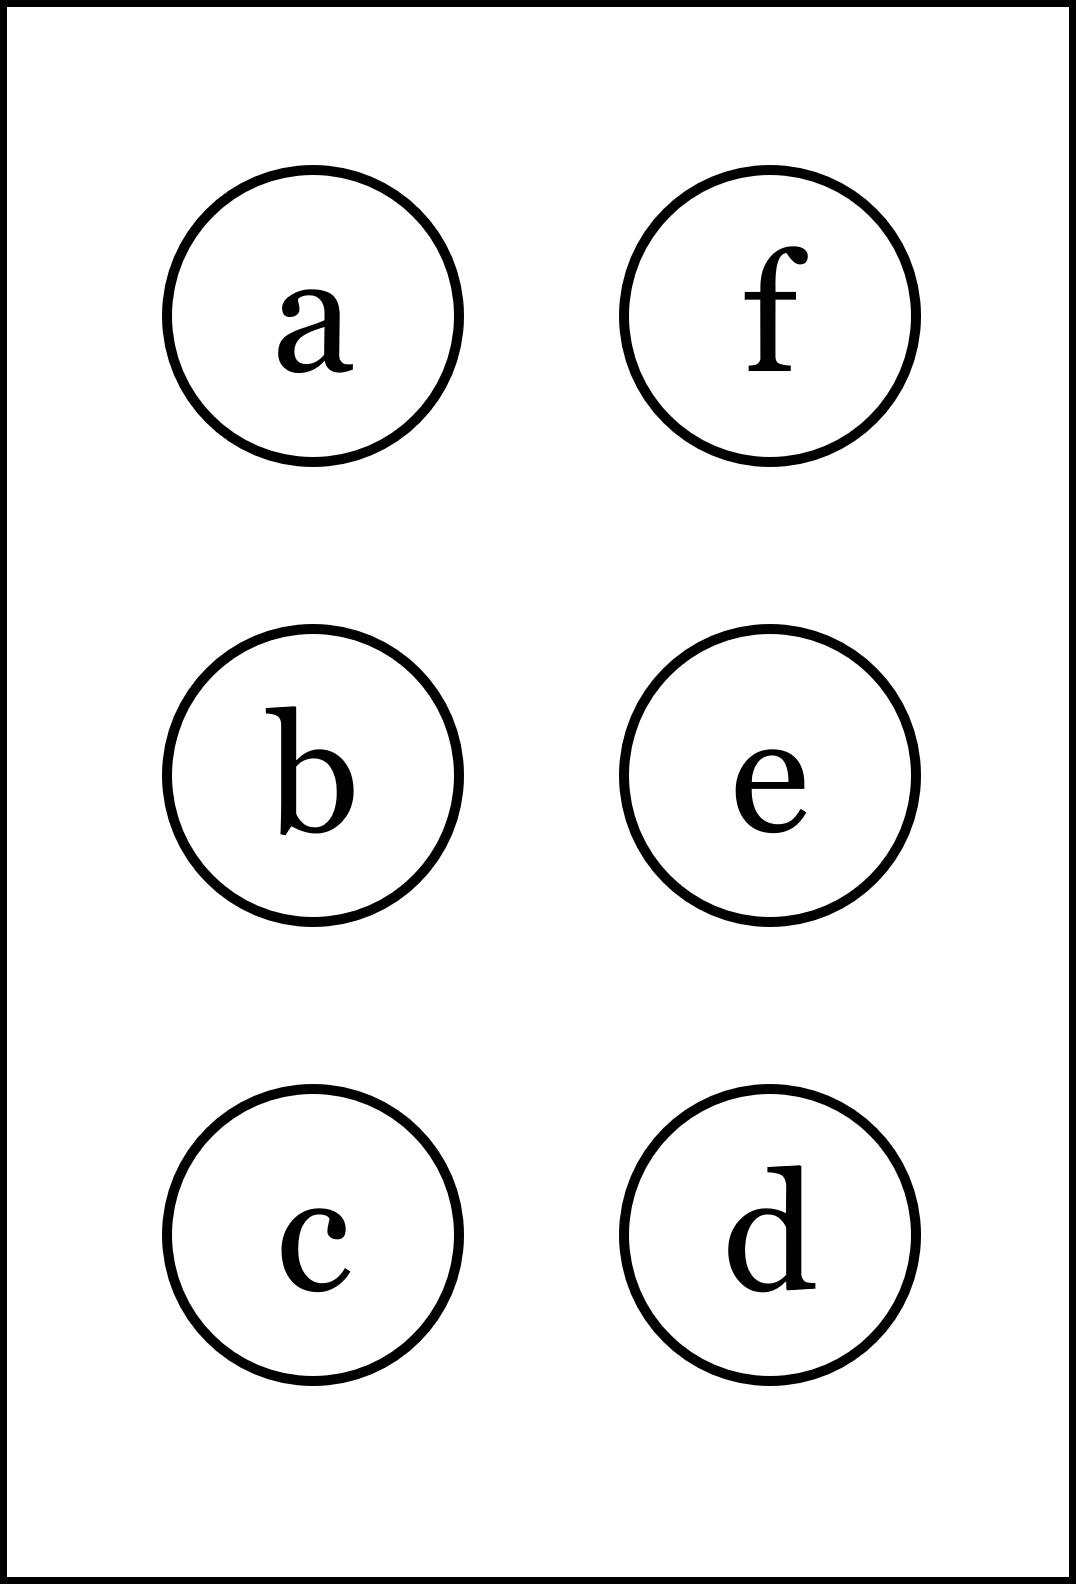
\includegraphics[height=40mm]{../images/braille.png}
{\small Písmeno Braillovej abecedy}
\end{center}
\end{minipage}
\end{center}
\end{minipage}
%
\end{tabular}
\newpage
\thispagestyle{empty}
\begin{tabular}{c:c}
\begin{minipage}[c][104.5mm][t]{0.5\linewidth}
\begin{center}
\vspace{7mm}
{\huge Kubická rovnice, skupina \textit{Delta $\delta$} -\romannumeral1}\\[5mm]
\textit{Jméno:}\phantom{xxxxxxxxxxxxxxxxxxxxxxxxxxxxxxxxxxxxxxxxxxxxxxxxxxxxxxxxxxxxxxxxx}\\[5mm]
\begin{minipage}{0.95\linewidth}
\begin{center}
\textbf{Vypočítej součet kořenů kubické rovnice.} Dvojitý kořen považuj do součtu za dva,\\trojitý kořen za tři. Pokud ti vyjde stejný výsledek jako je za otazníky, tak napravo\\barvi příslušející kroužek načerno. \textbf{Spolu odevzdejte výsledné slovo}.
\end{center}
\end{minipage}
\\[1mm]
\begin{minipage}{0.79\linewidth}
\begin{center}
\begin{varwidth}{\linewidth}
\begin{enumerate}
\Large
\item $-x^3+4x^2+5x=0$\quad \dotfill\; ???\;\dotfill \quad $4$
\item $-6x^3-6x^2+54x+54=0$\quad \dotfill\; ???\;\dotfill \quad $1$
\item $12x^3-58x^2-12x+10=0$\quad \dotfill\; ???\;\dotfill \quad $\nicefrac{25}{6}$
\item $20x^3-30x^2-20x+30=0$\quad \dotfill\; ???\;\dotfill \quad $\nicefrac{3}{2}$
\item \quad \dotfill\; ???\;\dotfill \quad nebarvi
\item \quad \dotfill\; ???\;\dotfill \quad vybarvi
\end{enumerate}
\end{varwidth}
\end{center}
\end{minipage}
\begin{minipage}{0.20\linewidth}
\begin{center}
{\Huge\bfseries 1.} \\[2mm]
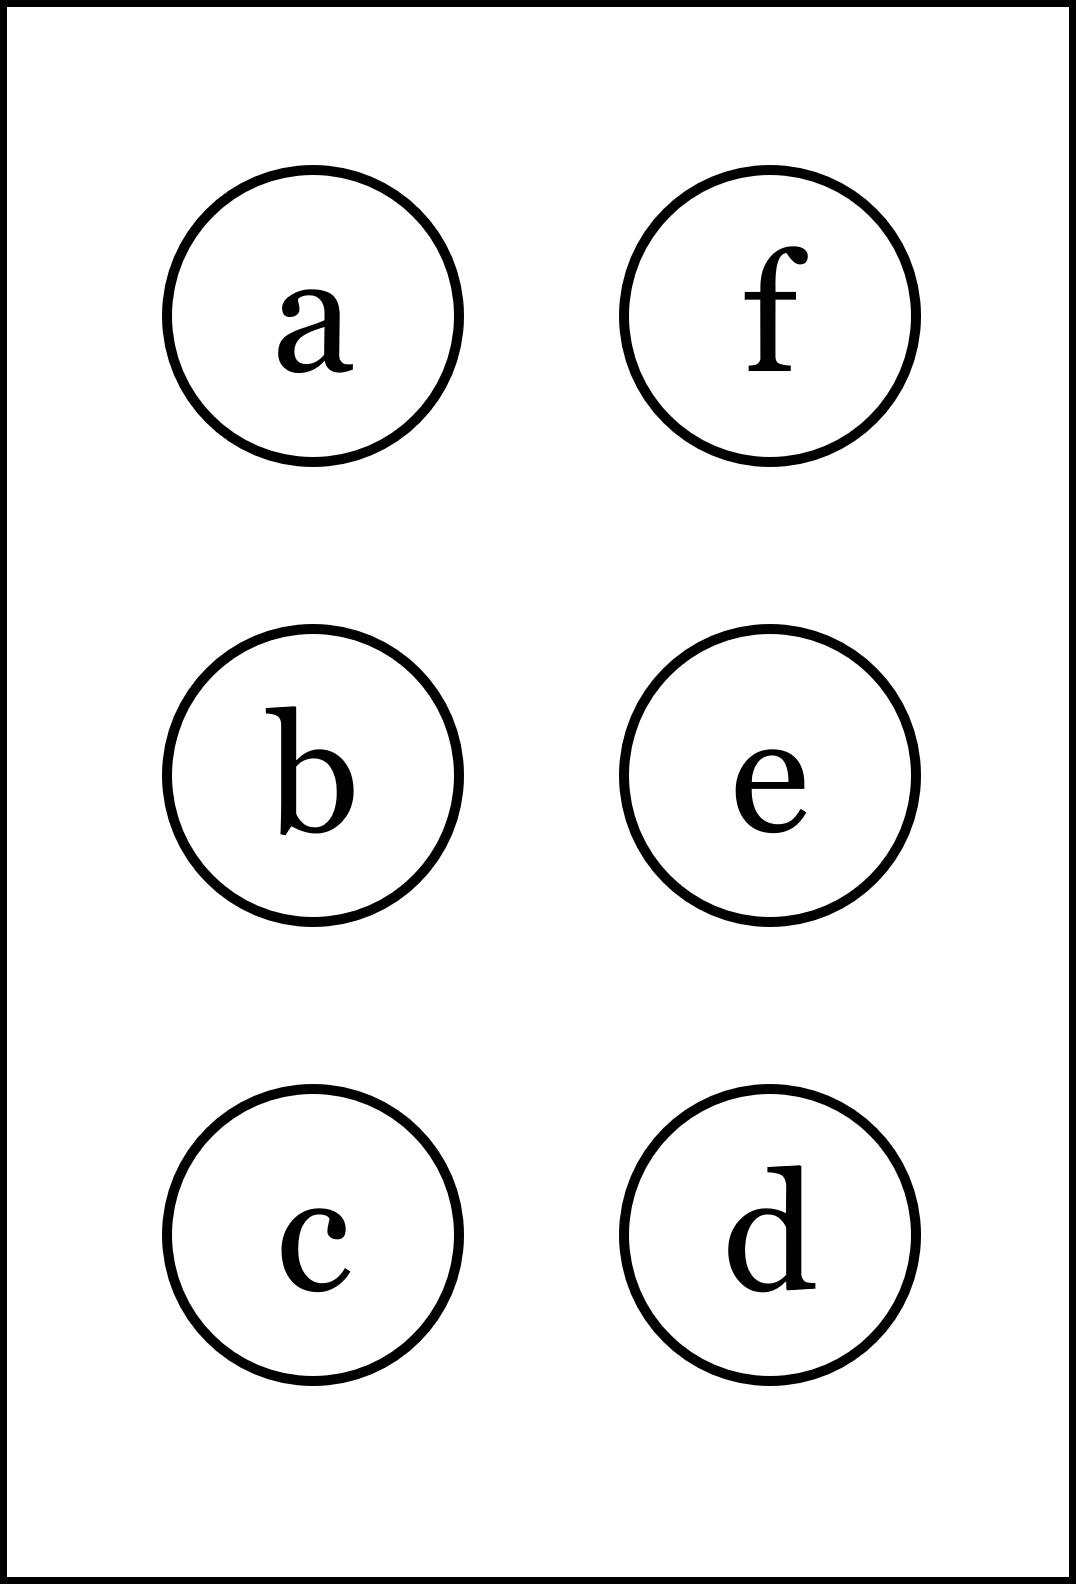
\includegraphics[height=40mm]{../images/braille.png}
{\small Písmeno Braillovej abecedy}
\end{center}
\end{minipage}
\end{center}
\end{minipage}
&
\begin{minipage}[c][104.5mm][t]{0.5\linewidth}
\begin{center}
\vspace{7mm}
{\huge Kubická rovnice, skupina \textit{Delta $\delta$} -\romannumeral2}\\[5mm]
\textit{Jméno:}\phantom{xxxxxxxxxxxxxxxxxxxxxxxxxxxxxxxxxxxxxxxxxxxxxxxxxxxxxxxxxxxxxxxxx}\\[5mm]
\begin{minipage}{0.95\linewidth}
\begin{center}
\textbf{Vypočítej součet kořenů kubické rovnice.} Dvojitý kořen považuj do součtu za dva,\\trojitý kořen za tři. Pokud ti vyjde stejný výsledek jako je za otazníky, tak napravo\\barvi příslušející kroužek načerno. \textbf{Spolu odevzdejte výsledné slovo}.
\end{center}
\end{minipage}
\\[1mm]
\begin{minipage}{0.79\linewidth}
\begin{center}
\begin{varwidth}{\linewidth}
\begin{enumerate}
\Large
\item $6x^3+12x^2-48x=0$\quad \dotfill\; ???\;\dotfill \quad $-6$
\item $-x^3+6x^2+9x-14=0$\quad \dotfill\; ???\;\dotfill \quad $-8$
\item $6x^3+19x^2-4x-21=0$\quad \dotfill\; ???\;\dotfill \quad $\nicefrac{-19}{6}$
\item $18x^3-12x^2-30x+24=0$\quad \dotfill\; ???\;\dotfill \quad $\nicefrac{-4}{3}$
\item \quad \dotfill\; ???\;\dotfill \quad nebarvi
\item \quad \dotfill\; ???\;\dotfill \quad vybarvi
\end{enumerate}
\end{varwidth}
\end{center}
\end{minipage}
\begin{minipage}{0.20\linewidth}
\begin{center}
{\Huge\bfseries 2.} \\[2mm]
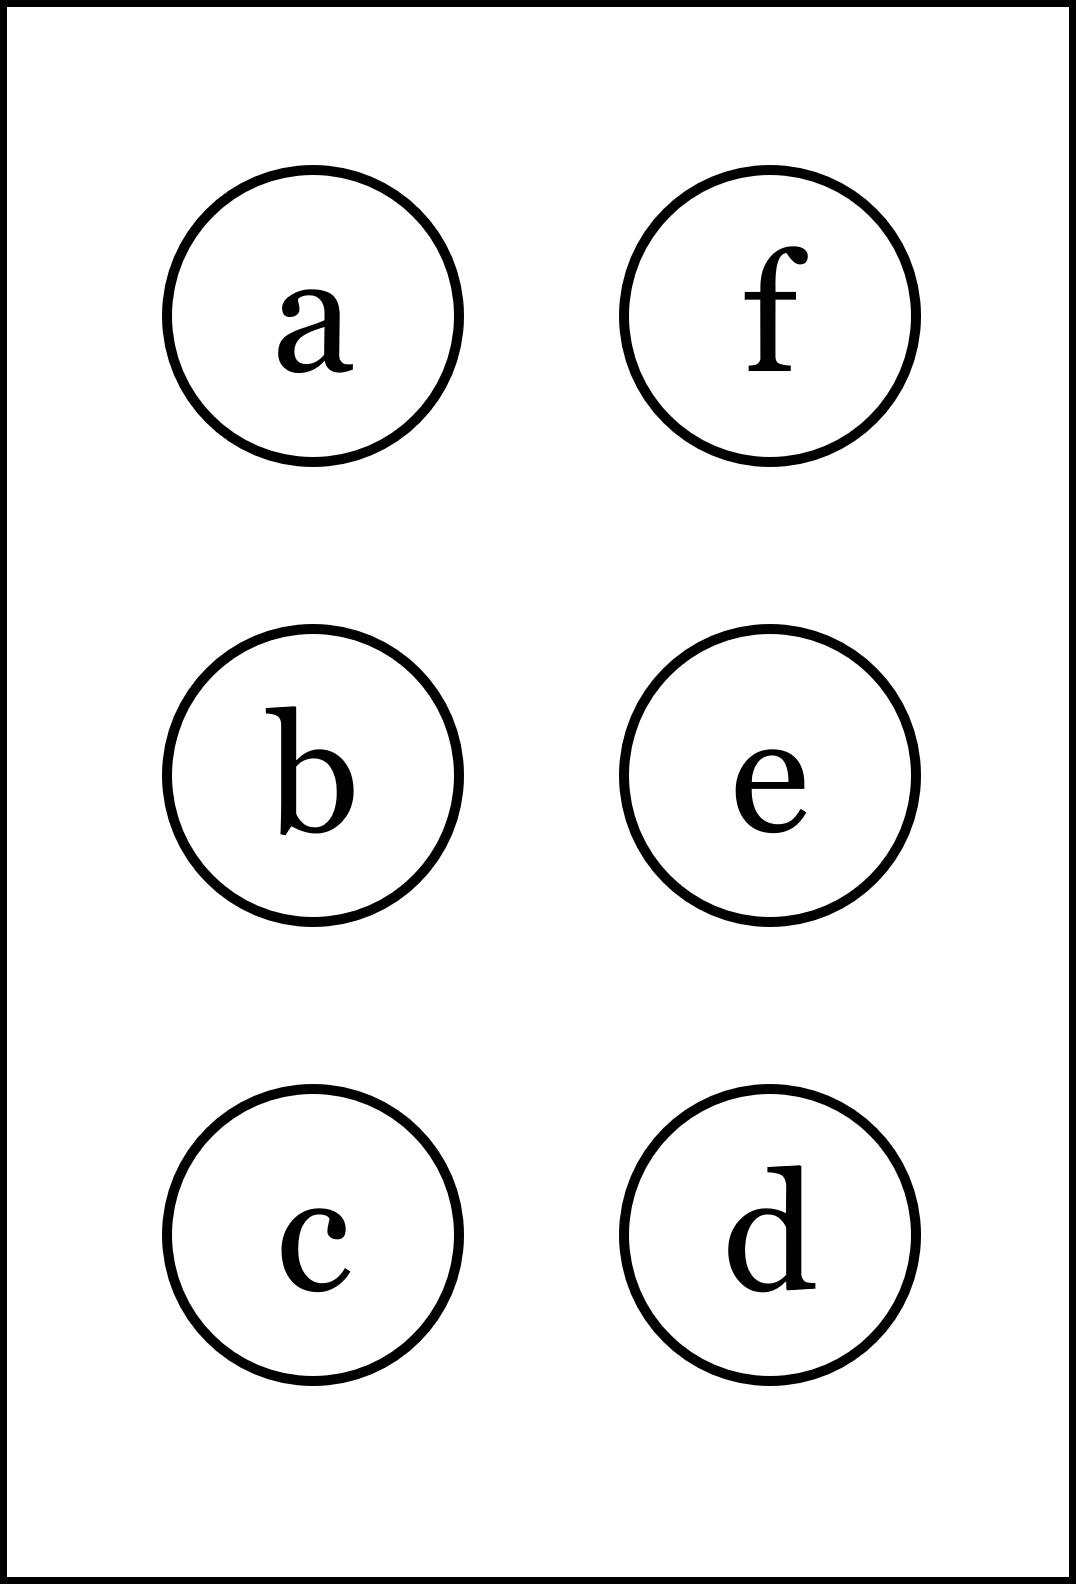
\includegraphics[height=40mm]{../images/braille.png}
{\small Písmeno Braillovej abecedy}
\end{center}
\end{minipage}
\end{center}
\end{minipage}
\\ \hdashline
\begin{minipage}[c][104.5mm][t]{0.5\linewidth}
\begin{center}
\vspace{7mm}
{\huge Kubická rovnice, skupina \textit{Delta $\delta$} -\romannumeral3}\\[5mm]
\textit{Jméno:}\phantom{xxxxxxxxxxxxxxxxxxxxxxxxxxxxxxxxxxxxxxxxxxxxxxxxxxxxxxxxxxxxxxxxx}\\[5mm]
\begin{minipage}{0.95\linewidth}
\begin{center}
\textbf{Vypočítej součet kořenů kubické rovnice.} Dvojitý kořen považuj do součtu za dva,\\trojitý kořen za tři. Pokud ti vyjde stejný výsledek jako je za otazníky, tak napravo\\barvi příslušející kroužek načerno. \textbf{Spolu odevzdejte výsledné slovo}.
\end{center}
\end{minipage}
\\[1mm]
\begin{minipage}{0.79\linewidth}
\begin{center}
\begin{varwidth}{\linewidth}
\begin{enumerate}
\Large
\item $-x^3-2x^2-x=0$\quad \dotfill\; ???\;\dotfill \quad $-2$
\item $-3x^3+9x^2+27x+15=0$\quad \dotfill\; ???\;\dotfill \quad $5$
\item $-24x^3-80x^2-72x-16=0$\quad \dotfill\; ???\;\dotfill \quad $\nicefrac{-10}{3}$
\item $4x^3-14x^2-28x-10=0$\quad \dotfill\; ???\;\dotfill \quad $\nicefrac{-13}{2}$
\item \quad \dotfill\; ???\;\dotfill \quad vybarvi
\item \quad \dotfill\; ???\;\dotfill \quad vybarvi
\end{enumerate}
\end{varwidth}
\end{center}
\end{minipage}
\begin{minipage}{0.20\linewidth}
\begin{center}
{\Huge\bfseries 3.} \\[2mm]
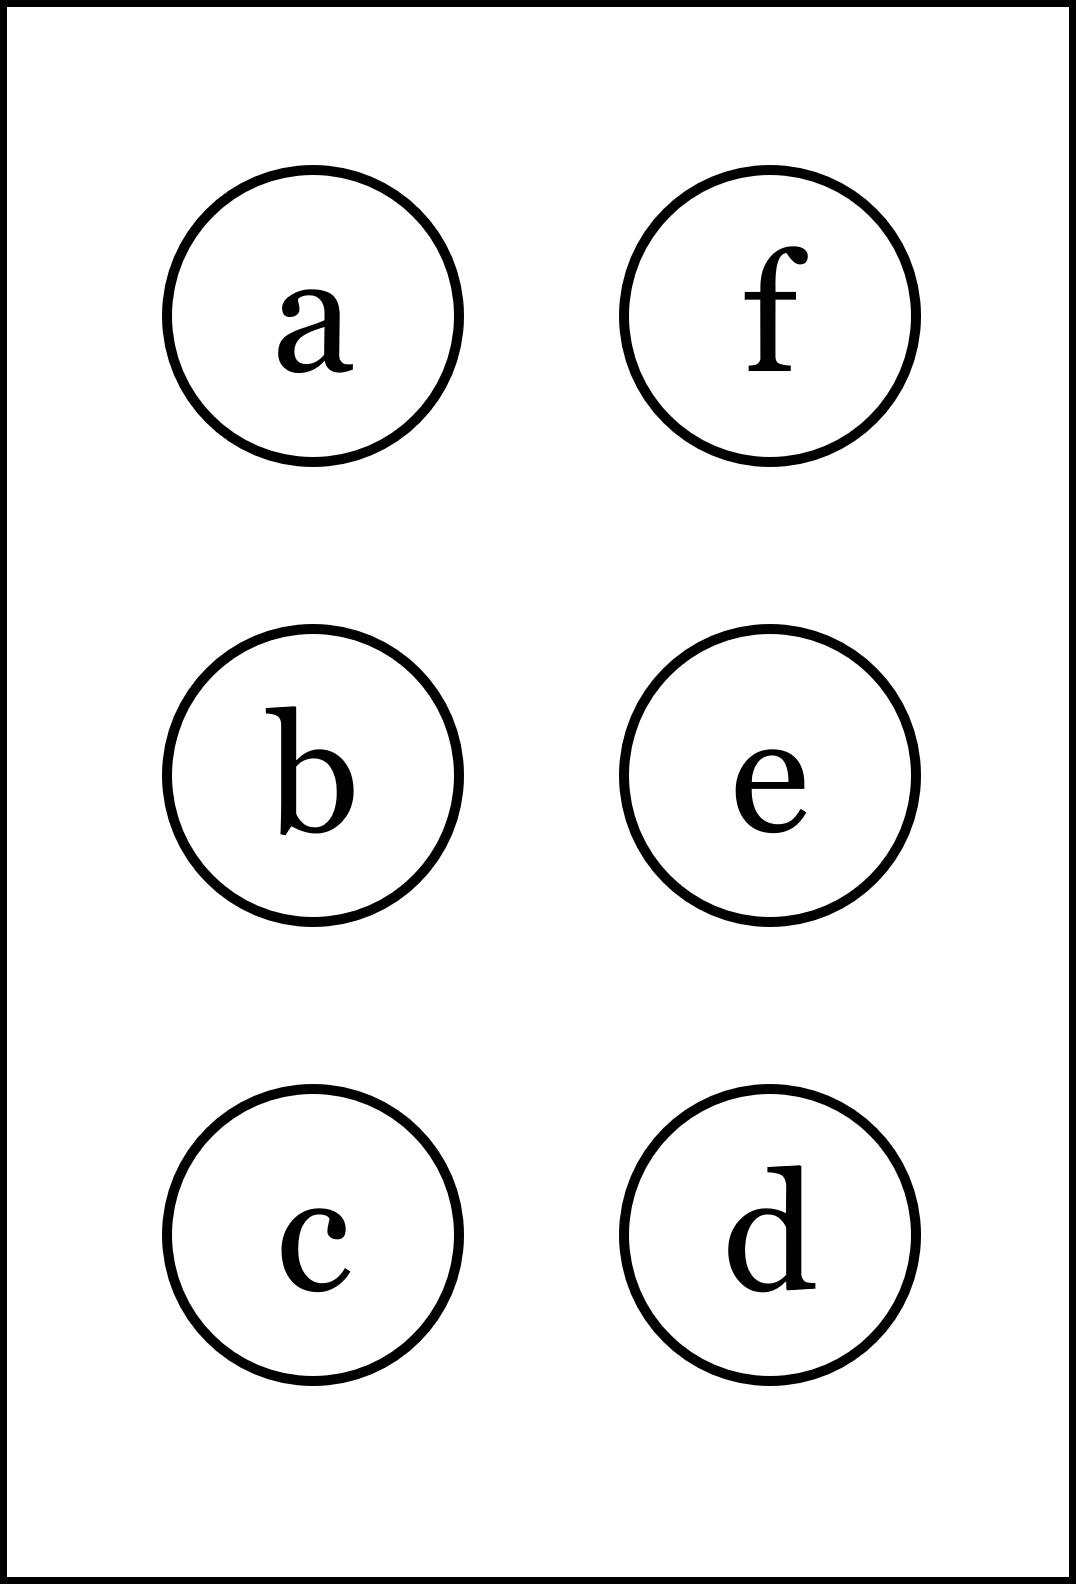
\includegraphics[height=40mm]{../images/braille.png}
{\small Písmeno Braillovej abecedy}
\end{center}
\end{minipage}
\end{center}
\end{minipage}
&
\begin{minipage}[c][104.5mm][t]{0.5\linewidth}
\begin{center}
\vspace{7mm}
{\huge Kubická rovnice, skupina \textit{Delta $\delta$} -\romannumeral4}\\[5mm]
\textit{Jméno:}\phantom{xxxxxxxxxxxxxxxxxxxxxxxxxxxxxxxxxxxxxxxxxxxxxxxxxxxxxxxxxxxxxxxxx}\\[5mm]
\begin{minipage}{0.95\linewidth}
\begin{center}
\textbf{Vypočítej součet kořenů kubické rovnice.} Dvojitý kořen považuj do součtu za dva,\\trojitý kořen za tři. Pokud ti vyjde stejný výsledek jako je za otazníky, tak napravo\\barvi příslušející kroužek načerno. \textbf{Spolu odevzdejte výsledné slovo}.
\end{center}
\end{minipage}
\\[1mm]
\begin{minipage}{0.79\linewidth}
\begin{center}
\begin{varwidth}{\linewidth}
\begin{enumerate}
\Large
\item $-2x^3+2x^2+12x=0$\quad \dotfill\; ???\;\dotfill \quad $1$
\item $-x^3+2x^2+x-2=0$\quad \dotfill\; ???\;\dotfill \quad $0$
\item $6x^3+19x^2+18x+5=0$\quad \dotfill\; ???\;\dotfill \quad $\nicefrac{-13}{6}$
\item $-9x^3+24x^2-9x-6=0$\quad \dotfill\; ???\;\dotfill \quad $\nicefrac{10}{3}$
\item \quad \dotfill\; ???\;\dotfill \quad nebarvi
\item \quad \dotfill\; ???\;\dotfill \quad nebarvi
\end{enumerate}
\end{varwidth}
\end{center}
\end{minipage}
\begin{minipage}{0.20\linewidth}
\begin{center}
{\Huge\bfseries 4.} \\[2mm]
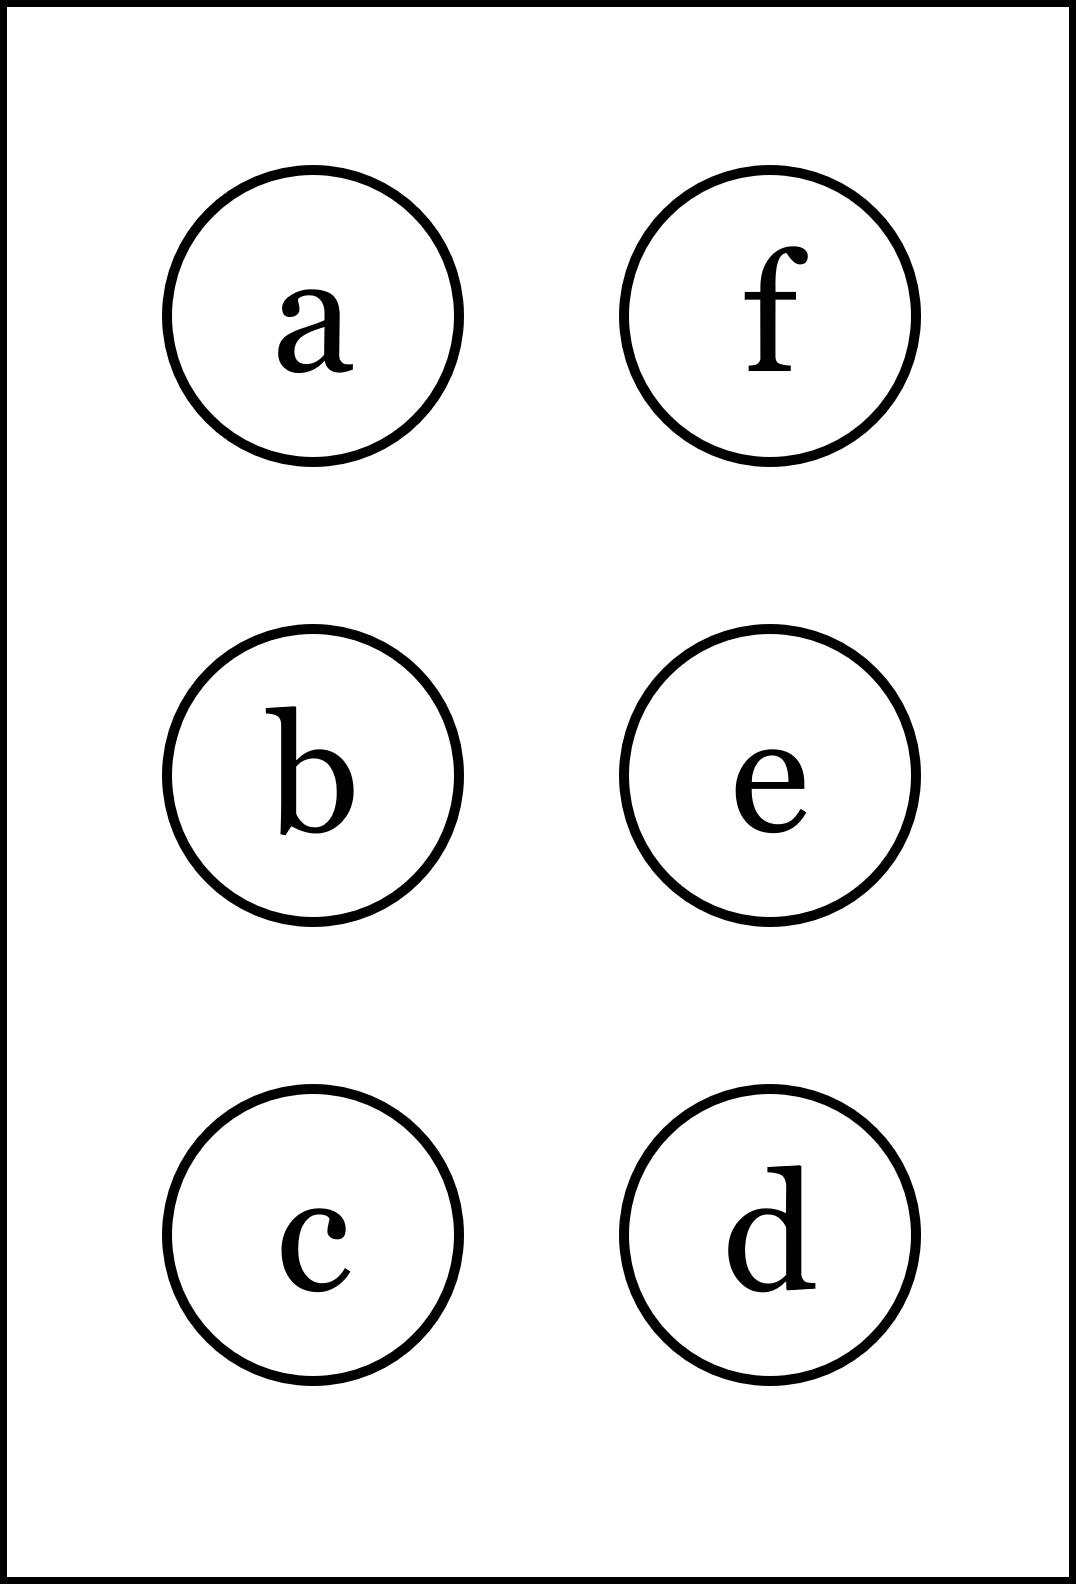
\includegraphics[height=40mm]{../images/braille.png}
{\small Písmeno Braillovej abecedy}
\end{center}
\end{minipage}
\end{center}
\end{minipage}
%
\end{tabular}
\newpage
\thispagestyle{empty}
\begin{tabular}{c:c}
\begin{minipage}[c][104.5mm][t]{0.5\linewidth}
\begin{center}
\vspace{7mm}
{\huge Kubická rovnice, skupina \textit{Epsilon $\epsilon$} -\romannumeral1}\\[5mm]
\textit{Jméno:}\phantom{xxxxxxxxxxxxxxxxxxxxxxxxxxxxxxxxxxxxxxxxxxxxxxxxxxxxxxxxxxxxxxxxx}\\[5mm]
\begin{minipage}{0.95\linewidth}
\begin{center}
\textbf{Vypočítej součet kořenů kubické rovnice.} Dvojitý kořen považuj do součtu za dva,\\trojitý kořen za tři. Pokud ti vyjde stejný výsledek jako je za otazníky, tak napravo\\barvi příslušející kroužek načerno. \textbf{Spolu odevzdejte výsledné slovo}.
\end{center}
\end{minipage}
\\[1mm]
\begin{minipage}{0.79\linewidth}
\begin{center}
\begin{varwidth}{\linewidth}
\begin{enumerate}
\Large
\item $-3x^3-3x^2+6x=0$\quad \dotfill\; ???\;\dotfill \quad $3$
\item $-5x^3-15x^2+30x+40=0$\quad \dotfill\; ???\;\dotfill \quad $5$
\item $2x^3+9x^2-6x-5=0$\quad \dotfill\; ???\;\dotfill \quad $\nicefrac{-9}{2}$
\item $-6x^3+46x^2-26x-14=0$\quad \dotfill\; ???\;\dotfill \quad $\nicefrac{23}{3}$
\item \quad \dotfill\; ???\;\dotfill \quad nebarvi
\item \quad \dotfill\; ???\;\dotfill \quad vybarvi
\end{enumerate}
\end{varwidth}
\end{center}
\end{minipage}
\begin{minipage}{0.20\linewidth}
\begin{center}
{\Huge\bfseries 1.} \\[2mm]
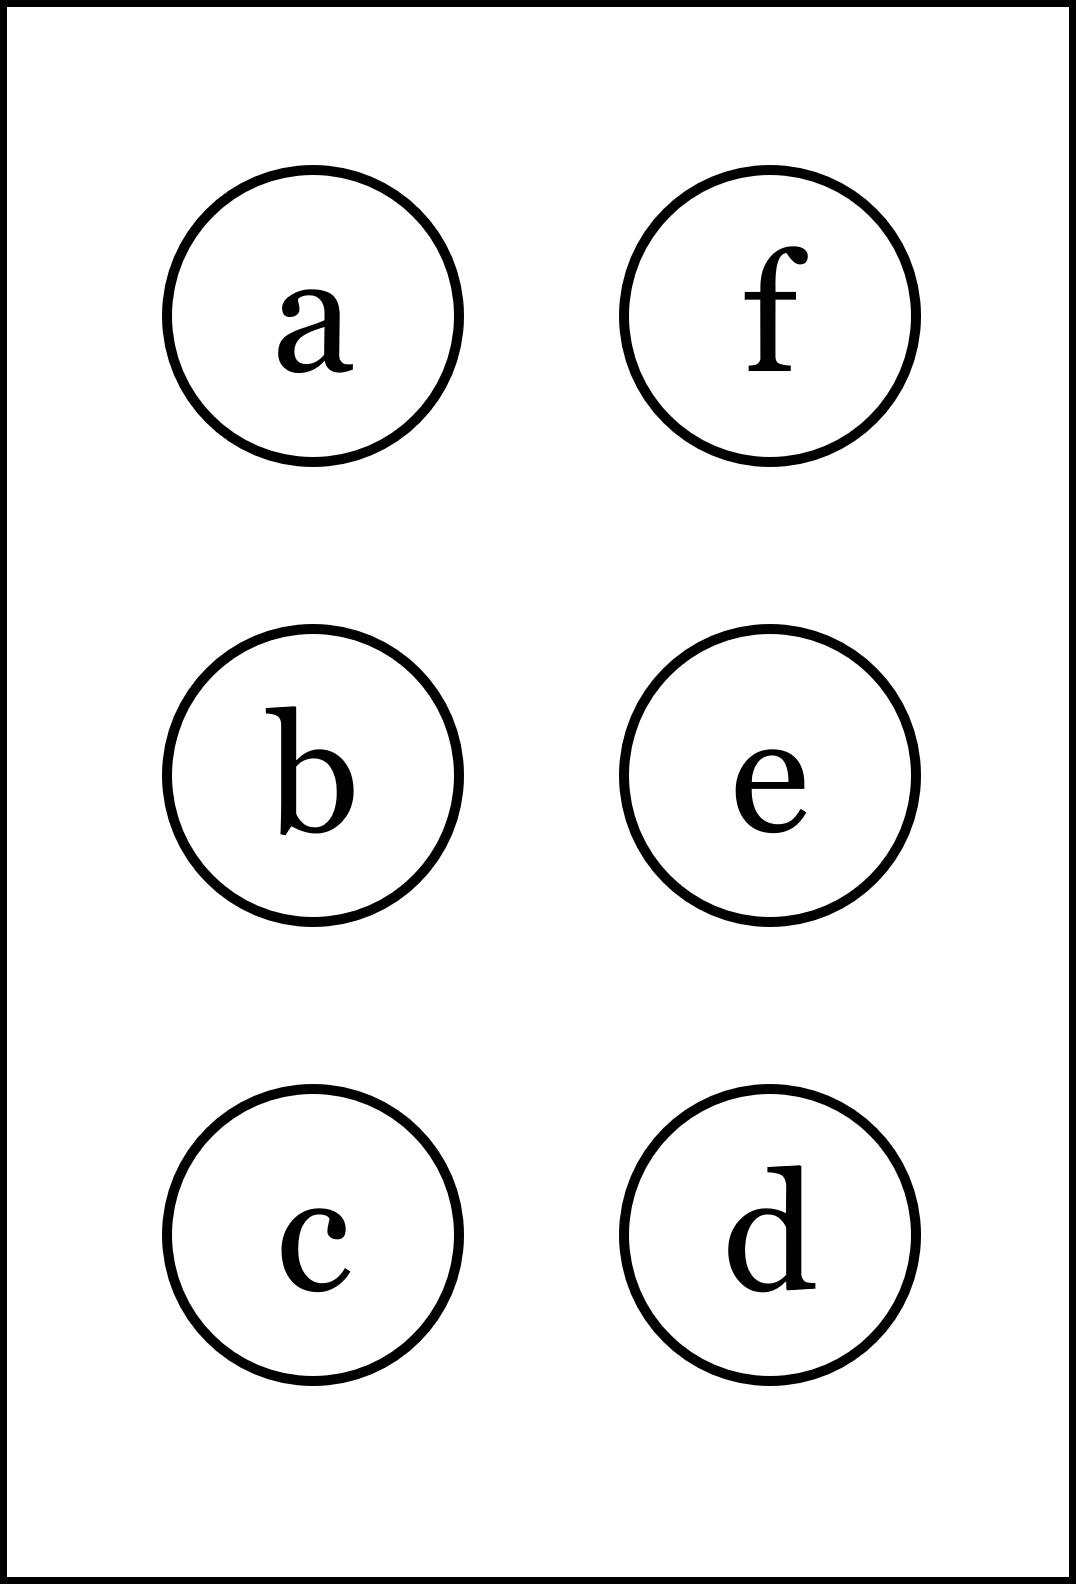
\includegraphics[height=40mm]{../images/braille.png}
{\small Písmeno Braillovej abecedy}
\end{center}
\end{minipage}
\end{center}
\end{minipage}
&
\begin{minipage}[c][104.5mm][t]{0.5\linewidth}
\begin{center}
\vspace{7mm}
{\huge Kubická rovnice, skupina \textit{Epsilon $\epsilon$} -\romannumeral2}\\[5mm]
\textit{Jméno:}\phantom{xxxxxxxxxxxxxxxxxxxxxxxxxxxxxxxxxxxxxxxxxxxxxxxxxxxxxxxxxxxxxxxxx}\\[5mm]
\begin{minipage}{0.95\linewidth}
\begin{center}
\textbf{Vypočítej součet kořenů kubické rovnice.} Dvojitý kořen považuj do součtu za dva,\\trojitý kořen za tři. Pokud ti vyjde stejný výsledek jako je za otazníky, tak napravo\\barvi příslušející kroužek načerno. \textbf{Spolu odevzdejte výsledné slovo}.
\end{center}
\end{minipage}
\\[1mm]
\begin{minipage}{0.79\linewidth}
\begin{center}
\begin{varwidth}{\linewidth}
\begin{enumerate}
\Large
\item $3x^3-9x^2+6x=0$\quad \dotfill\; ???\;\dotfill \quad $3$
\item $-x^3+9x^2-20x+12=0$\quad \dotfill\; ???\;\dotfill \quad $7$
\item $-24x^3-62x^2-30x-4=0$\quad \dotfill\; ???\;\dotfill \quad $\nicefrac{-31}{12}$
\item $-6x^3-7x^2+1=0$\quad \dotfill\; ???\;\dotfill \quad $\nicefrac{-11}{6}$
\item \quad \dotfill\; ???\;\dotfill \quad vybarvi
\item \quad \dotfill\; ???\;\dotfill \quad vybarvi
\end{enumerate}
\end{varwidth}
\end{center}
\end{minipage}
\begin{minipage}{0.20\linewidth}
\begin{center}
{\Huge\bfseries 2.} \\[2mm]
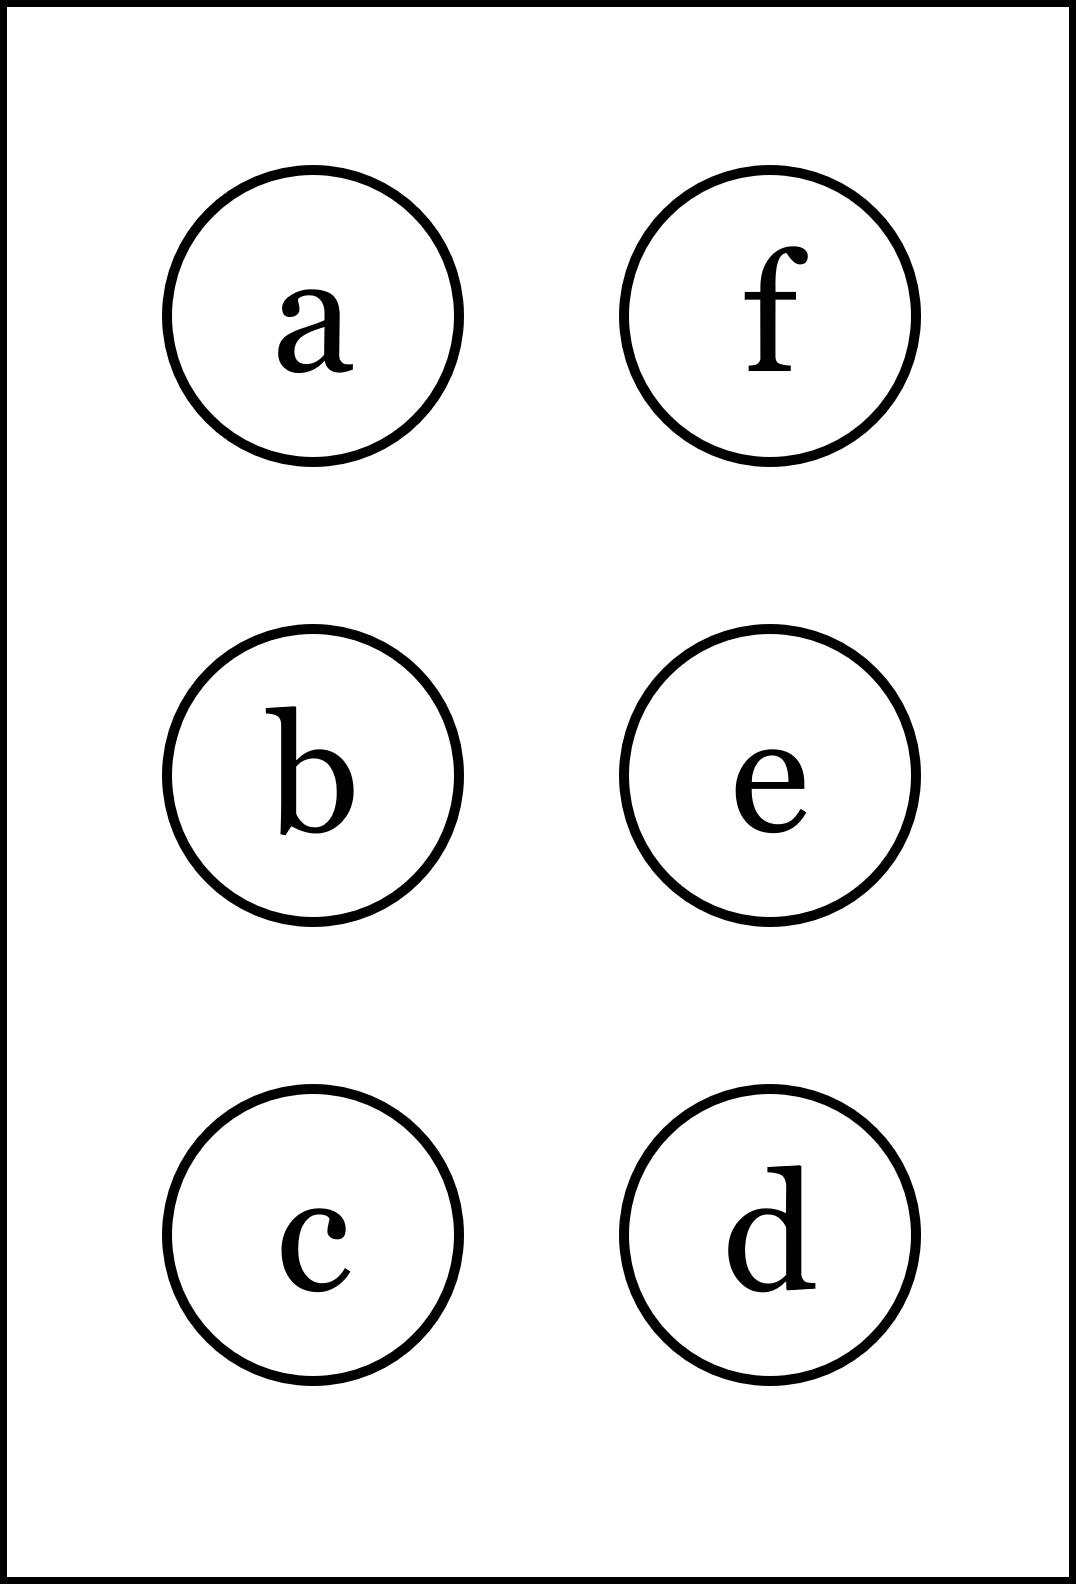
\includegraphics[height=40mm]{../images/braille.png}
{\small Písmeno Braillovej abecedy}
\end{center}
\end{minipage}
\end{center}
\end{minipage}
\\ \hdashline
\begin{minipage}[c][104.5mm][t]{0.5\linewidth}
\begin{center}
\vspace{7mm}
{\huge Kubická rovnice, skupina \textit{Epsilon $\epsilon$} -\romannumeral3}\\[5mm]
\textit{Jméno:}\phantom{xxxxxxxxxxxxxxxxxxxxxxxxxxxxxxxxxxxxxxxxxxxxxxxxxxxxxxxxxxxxxxxxx}\\[5mm]
\begin{minipage}{0.95\linewidth}
\begin{center}
\textbf{Vypočítej součet kořenů kubické rovnice.} Dvojitý kořen považuj do součtu za dva,\\trojitý kořen za tři. Pokud ti vyjde stejný výsledek jako je za otazníky, tak napravo\\barvi příslušející kroužek načerno. \textbf{Spolu odevzdejte výsledné slovo}.
\end{center}
\end{minipage}
\\[1mm]
\begin{minipage}{0.79\linewidth}
\begin{center}
\begin{varwidth}{\linewidth}
\begin{enumerate}
\Large
\item $x^3-x=0$\quad \dotfill\; ???\;\dotfill \quad $0$
\item $-2x^3-4x^2+22x+24=0$\quad \dotfill\; ???\;\dotfill \quad $-8$
\item $18x^3+21x^2+2x-1=0$\quad \dotfill\; ???\;\dotfill \quad $\nicefrac{-7}{6}$
\item $-4x^3-10x^2+22x-8=0$\quad \dotfill\; ???\;\dotfill \quad $\nicefrac{-7}{2}$
\item \quad \dotfill\; ???\;\dotfill \quad vybarvi
\item \quad \dotfill\; ???\;\dotfill \quad nebarvi
\end{enumerate}
\end{varwidth}
\end{center}
\end{minipage}
\begin{minipage}{0.20\linewidth}
\begin{center}
{\Huge\bfseries 3.} \\[2mm]
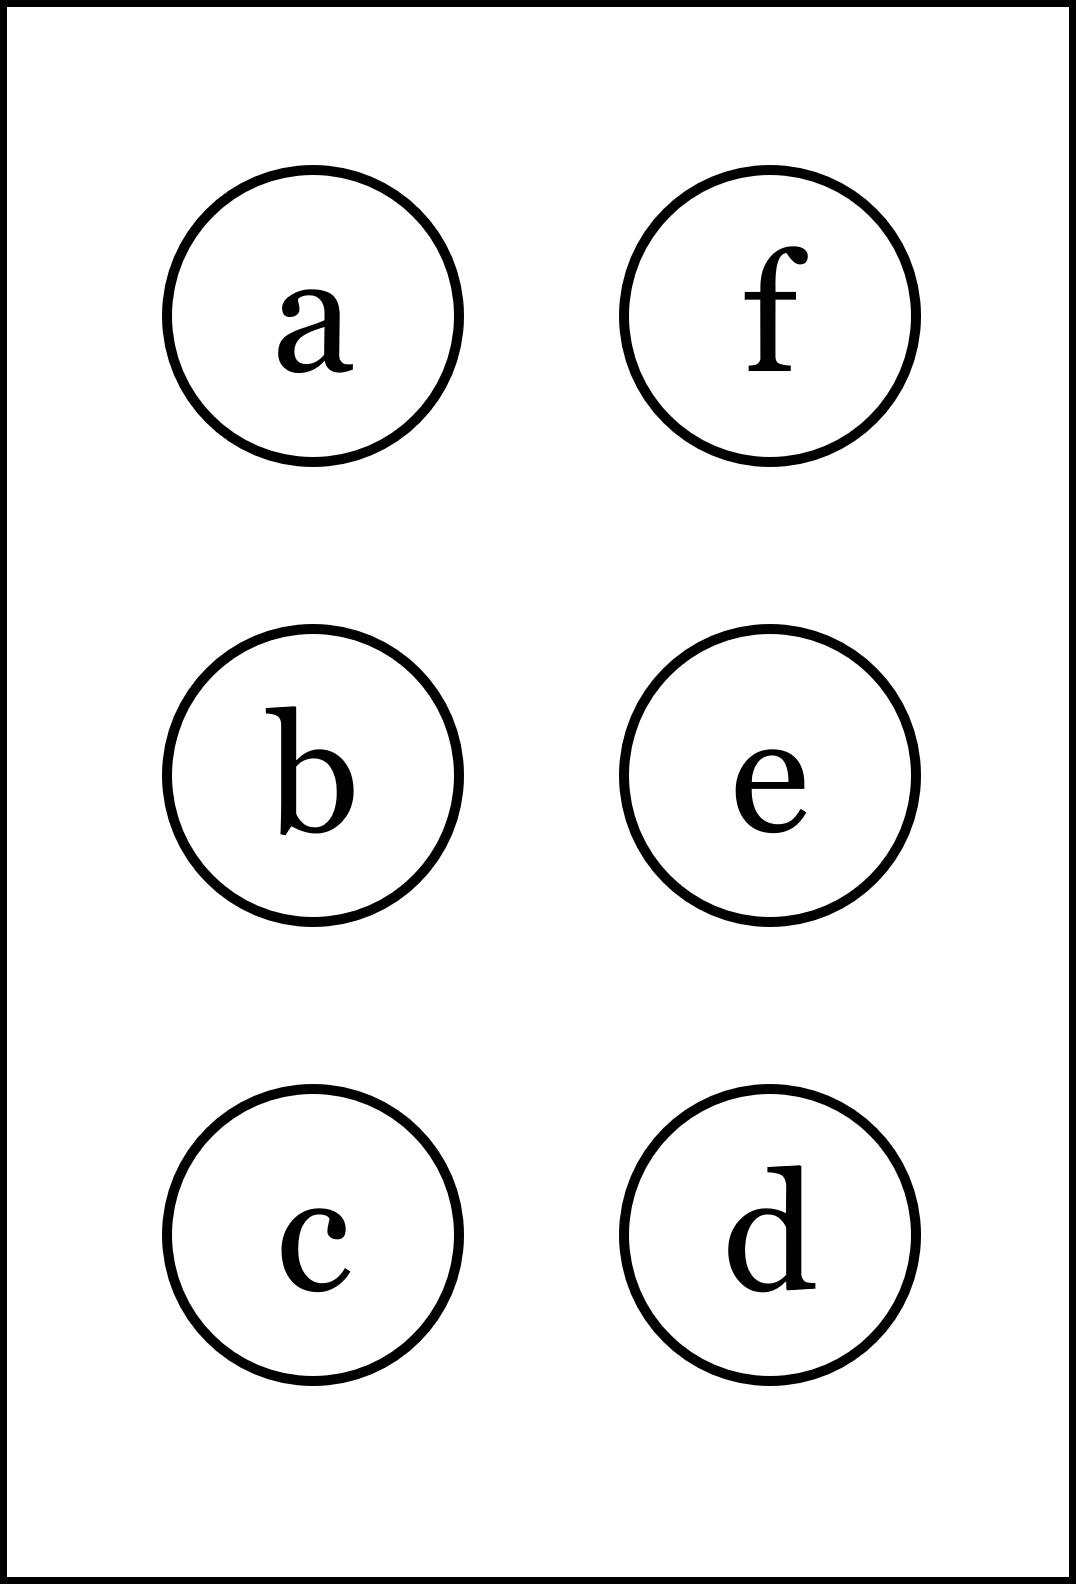
\includegraphics[height=40mm]{../images/braille.png}
{\small Písmeno Braillovej abecedy}
\end{center}
\end{minipage}
\end{center}
\end{minipage}
&
\begin{minipage}[c][104.5mm][t]{0.5\linewidth}
\begin{center}
\vspace{7mm}
{\huge Kubická rovnice, skupina \textit{Epsilon $\epsilon$} -\romannumeral4}\\[5mm]
\textit{Jméno:}\phantom{xxxxxxxxxxxxxxxxxxxxxxxxxxxxxxxxxxxxxxxxxxxxxxxxxxxxxxxxxxxxxxxxx}\\[5mm]
\begin{minipage}{0.95\linewidth}
\begin{center}
\textbf{Vypočítej součet kořenů kubické rovnice.} Dvojitý kořen považuj do součtu za dva,\\trojitý kořen za tři. Pokud ti vyjde stejný výsledek jako je za otazníky, tak napravo\\barvi příslušející kroužek načerno. \textbf{Spolu odevzdejte výsledné slovo}.
\end{center}
\end{minipage}
\\[1mm]
\begin{minipage}{0.79\linewidth}
\begin{center}
\begin{varwidth}{\linewidth}
\begin{enumerate}
\Large
\item $-x^3+7x^2-12x=0$\quad \dotfill\; ???\;\dotfill \quad $7$
\item $-4x^3+4x^2+40x+32=0$\quad \dotfill\; ???\;\dotfill \quad $1$
\item $-24x^3-22x^2+26x+20=0$\quad \dotfill\; ???\;\dotfill \quad $\nicefrac{-11}{12}$
\item $16x^3+12x^2-46x-12=0$\quad \dotfill\; ???\;\dotfill \quad $\nicefrac{-1}{4}$
\item \quad \dotfill\; ???\;\dotfill \quad vybarvi
\item \quad \dotfill\; ???\;\dotfill \quad nebarvi
\end{enumerate}
\end{varwidth}
\end{center}
\end{minipage}
\begin{minipage}{0.20\linewidth}
\begin{center}
{\Huge\bfseries 4.} \\[2mm]
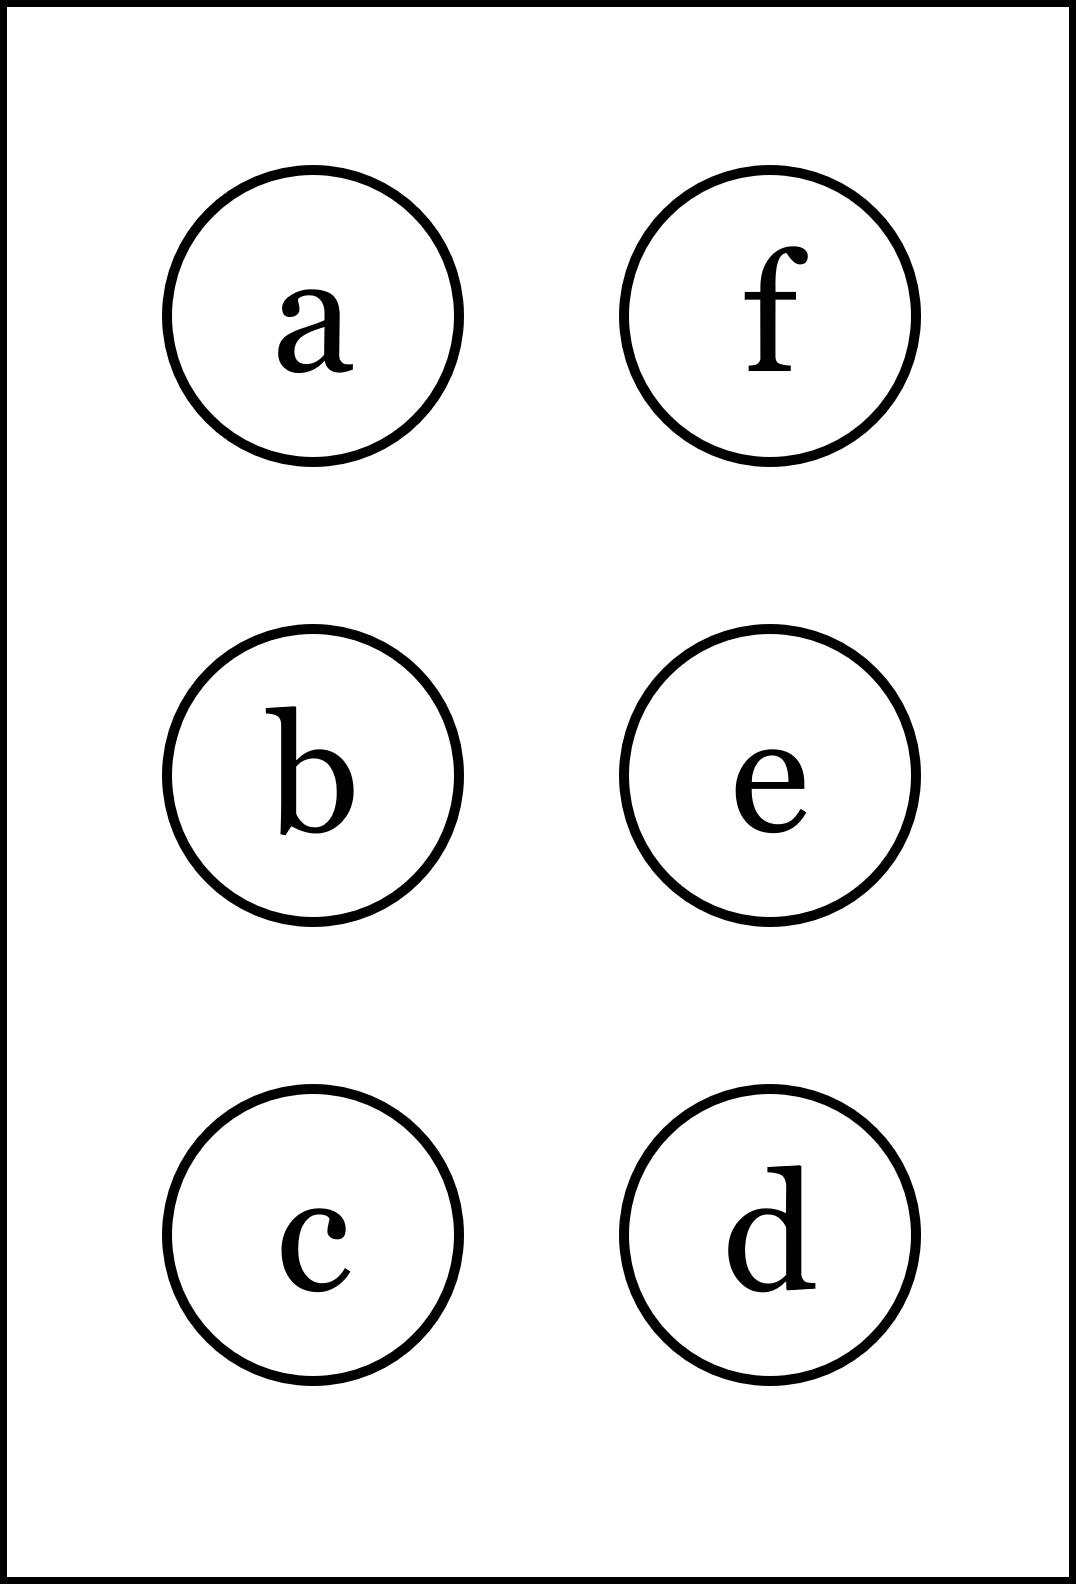
\includegraphics[height=40mm]{../images/braille.png}
{\small Písmeno Braillovej abecedy}
\end{center}
\end{minipage}
\end{center}
\end{minipage}
%
\end{tabular}
\newpage
\thispagestyle{empty}
\begin{tabular}{c:c}
\begin{minipage}[c][104.5mm][t]{0.5\linewidth}
\begin{center}
\vspace{7mm}
{\huge Kubická rovnice, skupina \textit{Zeta $\zeta$} -\romannumeral1}\\[5mm]
\textit{Jméno:}\phantom{xxxxxxxxxxxxxxxxxxxxxxxxxxxxxxxxxxxxxxxxxxxxxxxxxxxxxxxxxxxxxxxxx}\\[5mm]
\begin{minipage}{0.95\linewidth}
\begin{center}
\textbf{Vypočítej součet kořenů kubické rovnice.} Dvojitý kořen považuj do součtu za dva,\\trojitý kořen za tři. Pokud ti vyjde stejný výsledek jako je za otazníky, tak napravo\\barvi příslušející kroužek načerno. \textbf{Spolu odevzdejte výsledné slovo}.
\end{center}
\end{minipage}
\\[1mm]
\begin{minipage}{0.79\linewidth}
\begin{center}
\begin{varwidth}{\linewidth}
\begin{enumerate}
\Large
\item $x^3+7x^2+12x=0$\quad \dotfill\; ???\;\dotfill \quad $-7$
\item $3x^3-12x^2-3x+12=0$\quad \dotfill\; ???\;\dotfill \quad $2$
\item $-2x^3+6x^2+44x-48=0$\quad \dotfill\; ???\;\dotfill \quad $11$
\item $10x^3-61x^2+4x+12=0$\quad \dotfill\; ???\;\dotfill \quad $\nicefrac{69}{10}$
\item \quad \dotfill\; ???\;\dotfill \quad vybarvi
\item \quad \dotfill\; ???\;\dotfill \quad nebarvi
\end{enumerate}
\end{varwidth}
\end{center}
\end{minipage}
\begin{minipage}{0.20\linewidth}
\begin{center}
{\Huge\bfseries 1.} \\[2mm]
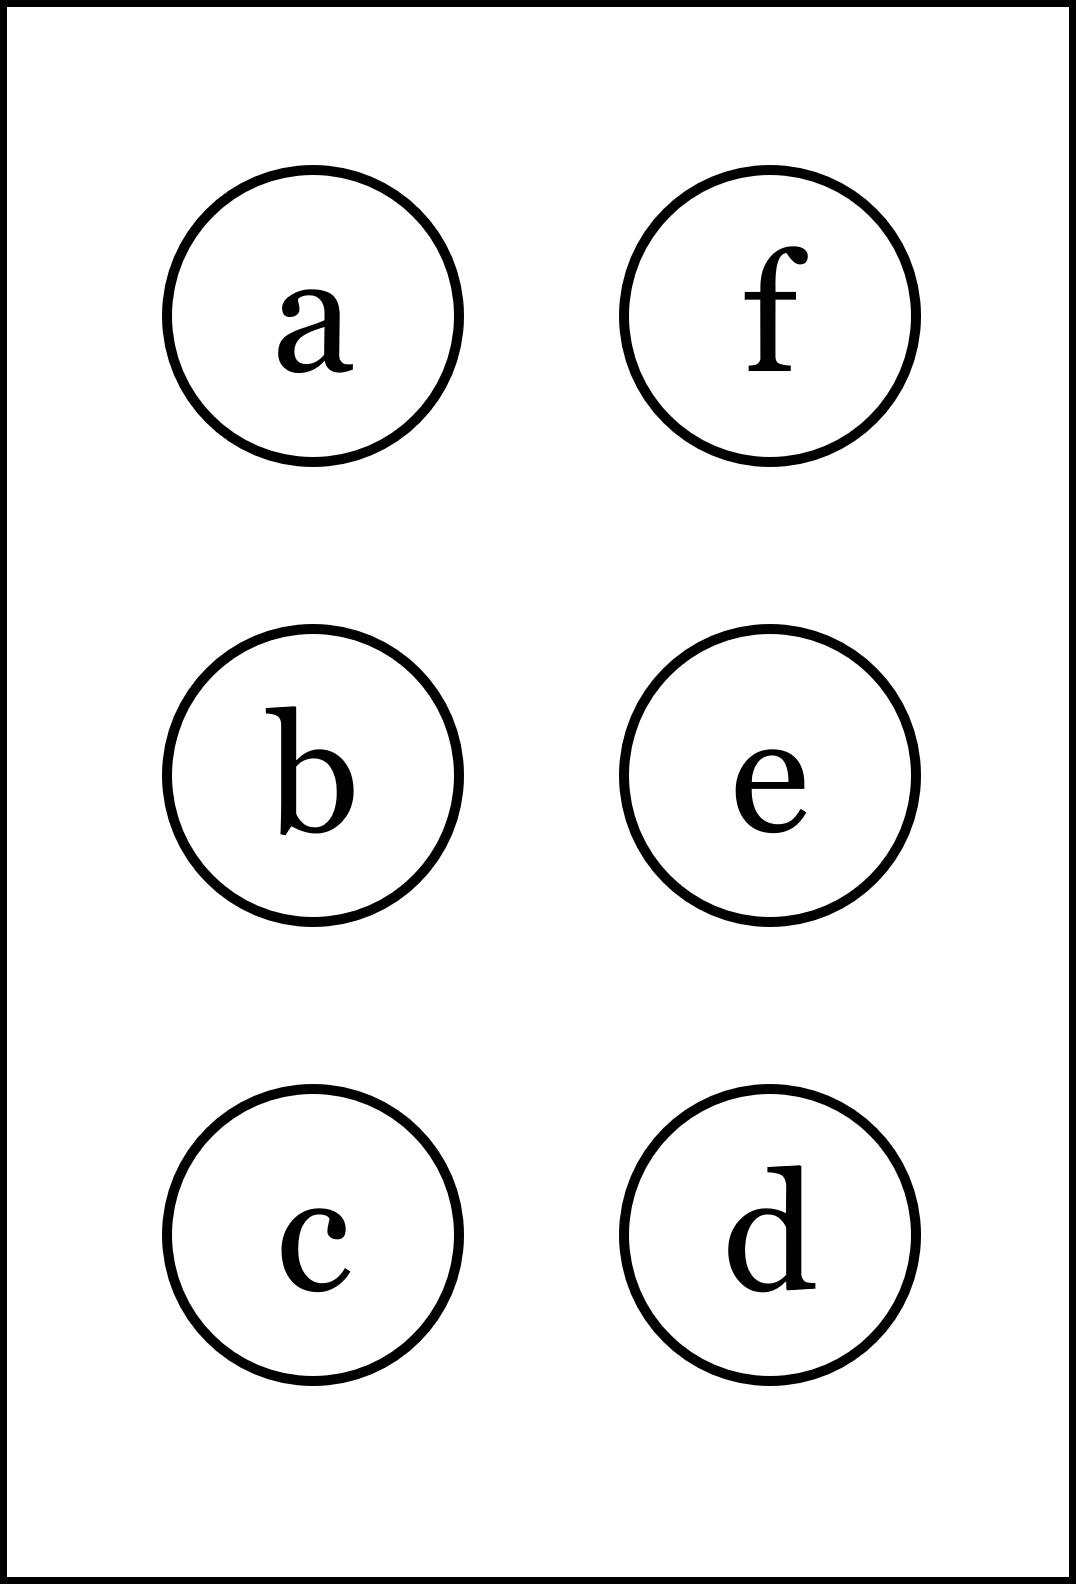
\includegraphics[height=40mm]{../images/braille.png}
{\small Písmeno Braillovej abecedy}
\end{center}
\end{minipage}
\end{center}
\end{minipage}
&
\begin{minipage}[c][104.5mm][t]{0.5\linewidth}
\begin{center}
\vspace{7mm}
{\huge Kubická rovnice, skupina \textit{Zeta $\zeta$} -\romannumeral2}\\[5mm]
\textit{Jméno:}\phantom{xxxxxxxxxxxxxxxxxxxxxxxxxxxxxxxxxxxxxxxxxxxxxxxxxxxxxxxxxxxxxxxxx}\\[5mm]
\begin{minipage}{0.95\linewidth}
\begin{center}
\textbf{Vypočítej součet kořenů kubické rovnice.} Dvojitý kořen považuj do součtu za dva,\\trojitý kořen za tři. Pokud ti vyjde stejný výsledek jako je za otazníky, tak napravo\\barvi příslušející kroužek načerno. \textbf{Spolu odevzdejte výsledné slovo}.
\end{center}
\end{minipage}
\\[1mm]
\begin{minipage}{0.79\linewidth}
\begin{center}
\begin{varwidth}{\linewidth}
\begin{enumerate}
\Large
\item $x^3+2x^2-15x=0$\quad \dotfill\; ???\;\dotfill \quad $-2$
\item $x^3-11x^2+26x-16=0$\quad \dotfill\; ???\;\dotfill \quad $11$
\item $25x^3-20x^2-55x-10=0$\quad \dotfill\; ???\;\dotfill \quad $\nicefrac{4}{5}$
\item $-14x^3+42x^2+14x-42=0$\quad \dotfill\; ???\;\dotfill \quad $5$
\item \quad \dotfill\; ???\;\dotfill \quad nebarvi
\item \quad \dotfill\; ???\;\dotfill \quad vybarvi
\end{enumerate}
\end{varwidth}
\end{center}
\end{minipage}
\begin{minipage}{0.20\linewidth}
\begin{center}
{\Huge\bfseries 2.} \\[2mm]
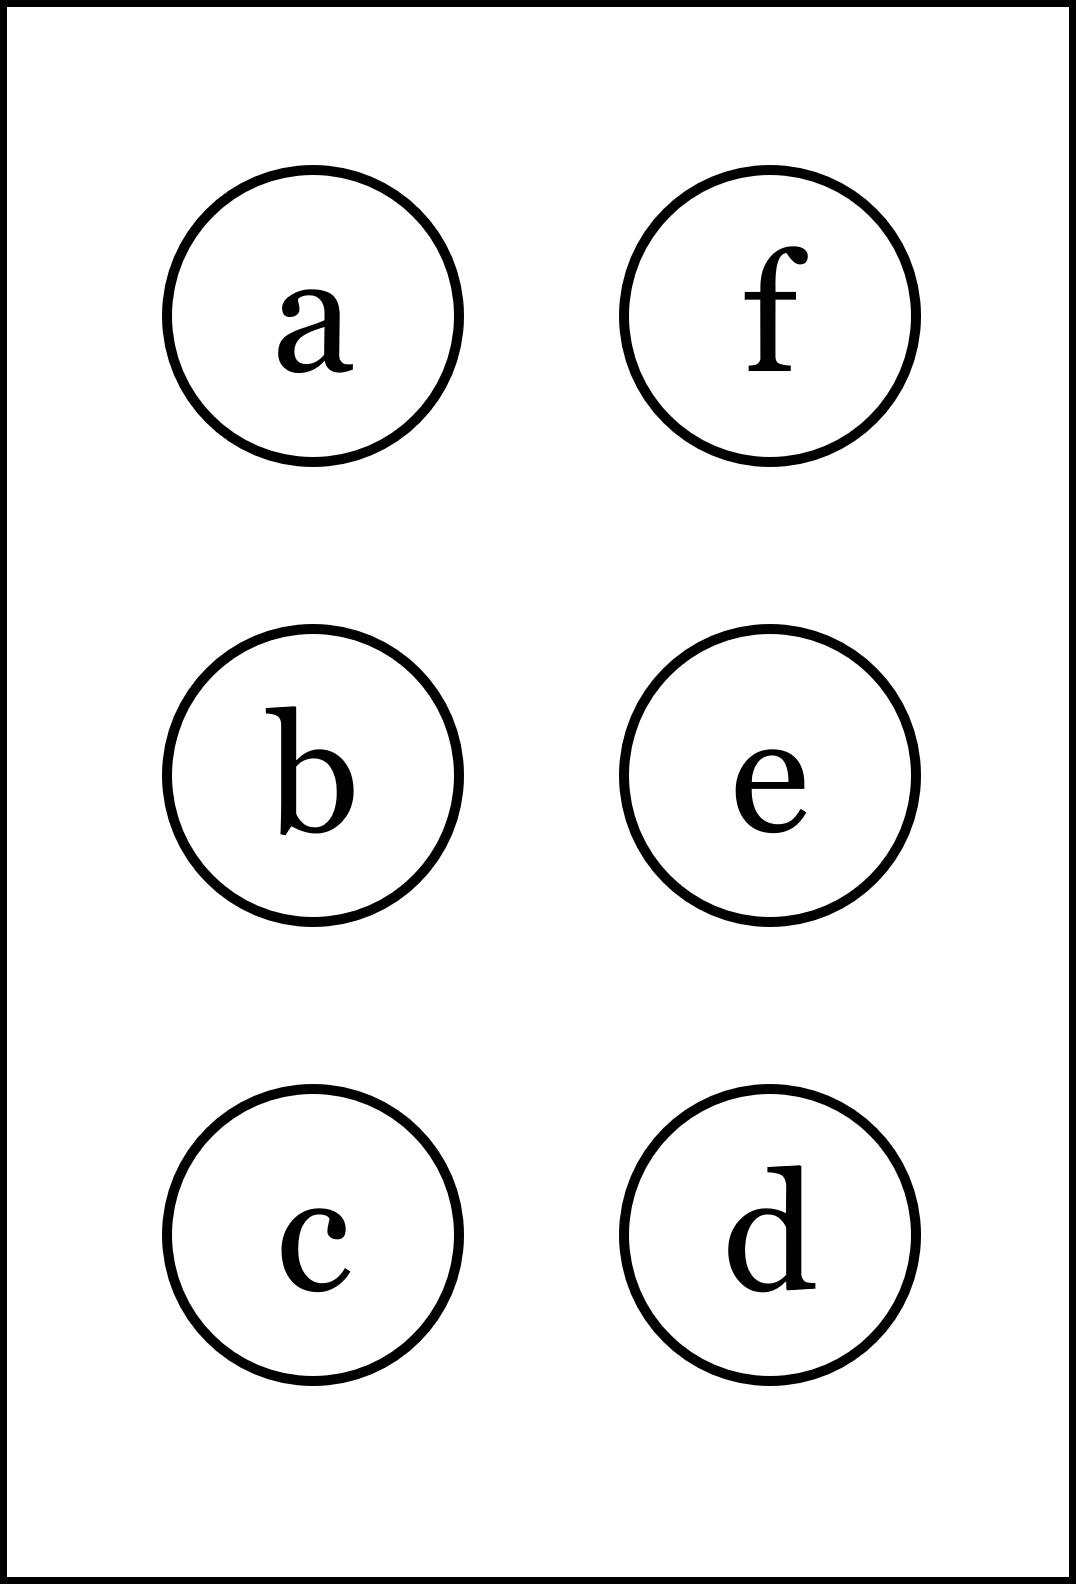
\includegraphics[height=40mm]{../images/braille.png}
{\small Písmeno Braillovej abecedy}
\end{center}
\end{minipage}
\end{center}
\end{minipage}
\\ \hdashline
\begin{minipage}[c][104.5mm][t]{0.5\linewidth}
\begin{center}
\vspace{7mm}
{\huge Kubická rovnice, skupina \textit{Zeta $\zeta$} -\romannumeral3}\\[5mm]
\textit{Jméno:}\phantom{xxxxxxxxxxxxxxxxxxxxxxxxxxxxxxxxxxxxxxxxxxxxxxxxxxxxxxxxxxxxxxxxx}\\[5mm]
\begin{minipage}{0.95\linewidth}
\begin{center}
\textbf{Vypočítej součet kořenů kubické rovnice.} Dvojitý kořen považuj do součtu za dva,\\trojitý kořen za tři. Pokud ti vyjde stejný výsledek jako je za otazníky, tak napravo\\barvi příslušející kroužek načerno. \textbf{Spolu odevzdejte výsledné slovo}.
\end{center}
\end{minipage}
\\[1mm]
\begin{minipage}{0.79\linewidth}
\begin{center}
\begin{varwidth}{\linewidth}
\begin{enumerate}
\Large
\item $-8x^3+16x^2+24x=0$\quad \dotfill\; ???\;\dotfill \quad $2$
\item $-x^3+8x^2-9x-18=0$\quad \dotfill\; ???\;\dotfill \quad $10$
\item $-12x^3+x^2+38x-24=0$\quad \dotfill\; ???\;\dotfill \quad $\nicefrac{1}{12}$
\item $-3x^3-17x^2-18x+8=0$\quad \dotfill\; ???\;\dotfill \quad $\nicefrac{-5}{3}$
\item \quad \dotfill\; ???\;\dotfill \quad vybarvi
\item \quad \dotfill\; ???\;\dotfill \quad nebarvi
\end{enumerate}
\end{varwidth}
\end{center}
\end{minipage}
\begin{minipage}{0.20\linewidth}
\begin{center}
{\Huge\bfseries 3.} \\[2mm]
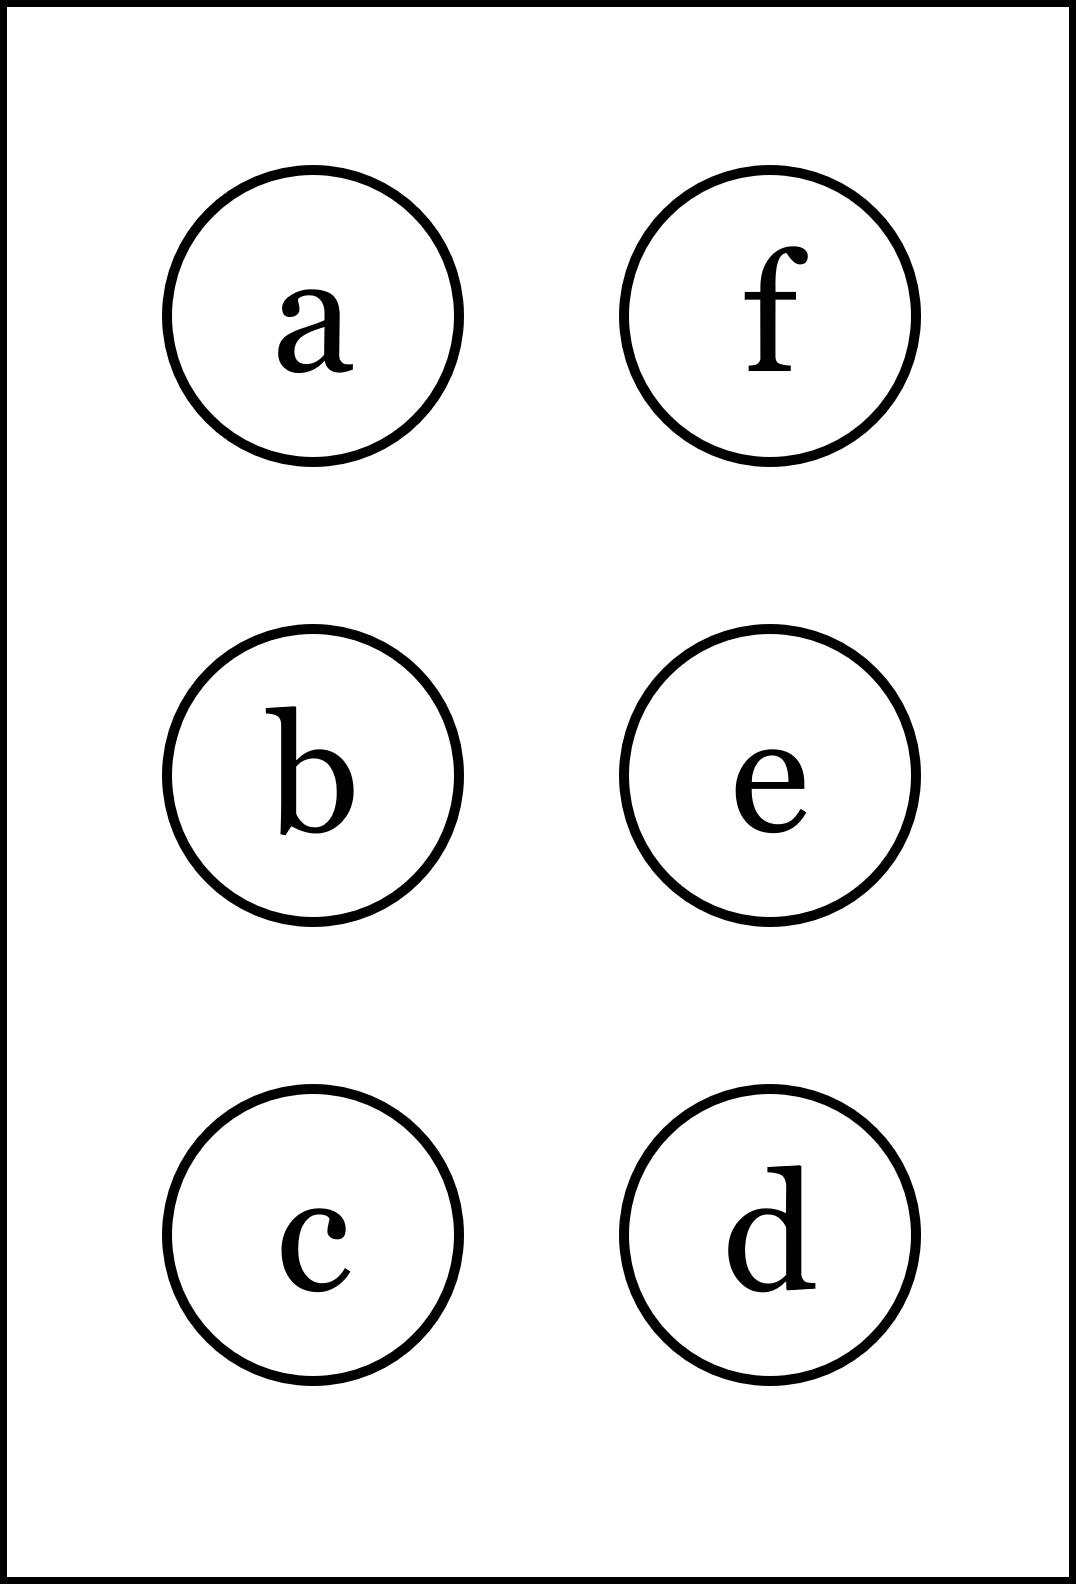
\includegraphics[height=40mm]{../images/braille.png}
{\small Písmeno Braillovej abecedy}
\end{center}
\end{minipage}
\end{center}
\end{minipage}
&
\begin{minipage}[c][104.5mm][t]{0.5\linewidth}
\begin{center}
\vspace{7mm}
{\huge Kubická rovnice, skupina \textit{Zeta $\zeta$} -\romannumeral4}\\[5mm]
\textit{Jméno:}\phantom{xxxxxxxxxxxxxxxxxxxxxxxxxxxxxxxxxxxxxxxxxxxxxxxxxxxxxxxxxxxxxxxxx}\\[5mm]
\begin{minipage}{0.95\linewidth}
\begin{center}
\textbf{Vypočítej součet kořenů kubické rovnice.} Dvojitý kořen považuj do součtu za dva,\\trojitý kořen za tři. Pokud ti vyjde stejný výsledek jako je za otazníky, tak napravo\\barvi příslušející kroužek načerno. \textbf{Spolu odevzdejte výsledné slovo}.
\end{center}
\end{minipage}
\\[1mm]
\begin{minipage}{0.79\linewidth}
\begin{center}
\begin{varwidth}{\linewidth}
\begin{enumerate}
\Large
\item $2x^3-8x^2+8x=0$\quad \dotfill\; ???\;\dotfill \quad $0$
\item $5x^3-15x^2-30x+40=0$\quad \dotfill\; ???\;\dotfill \quad $3$
\item $14x^3-26x^2-16x+24=0$\quad \dotfill\; ???\;\dotfill \quad $\nicefrac{13}{7}$
\item $-x^3+3x^2+16x+12=0$\quad \dotfill\; ???\;\dotfill \quad $5$
\item \quad \dotfill\; ???\;\dotfill \quad nebarvi
\item \quad \dotfill\; ???\;\dotfill \quad vybarvi
\end{enumerate}
\end{varwidth}
\end{center}
\end{minipage}
\begin{minipage}{0.20\linewidth}
\begin{center}
{\Huge\bfseries 4.} \\[2mm]
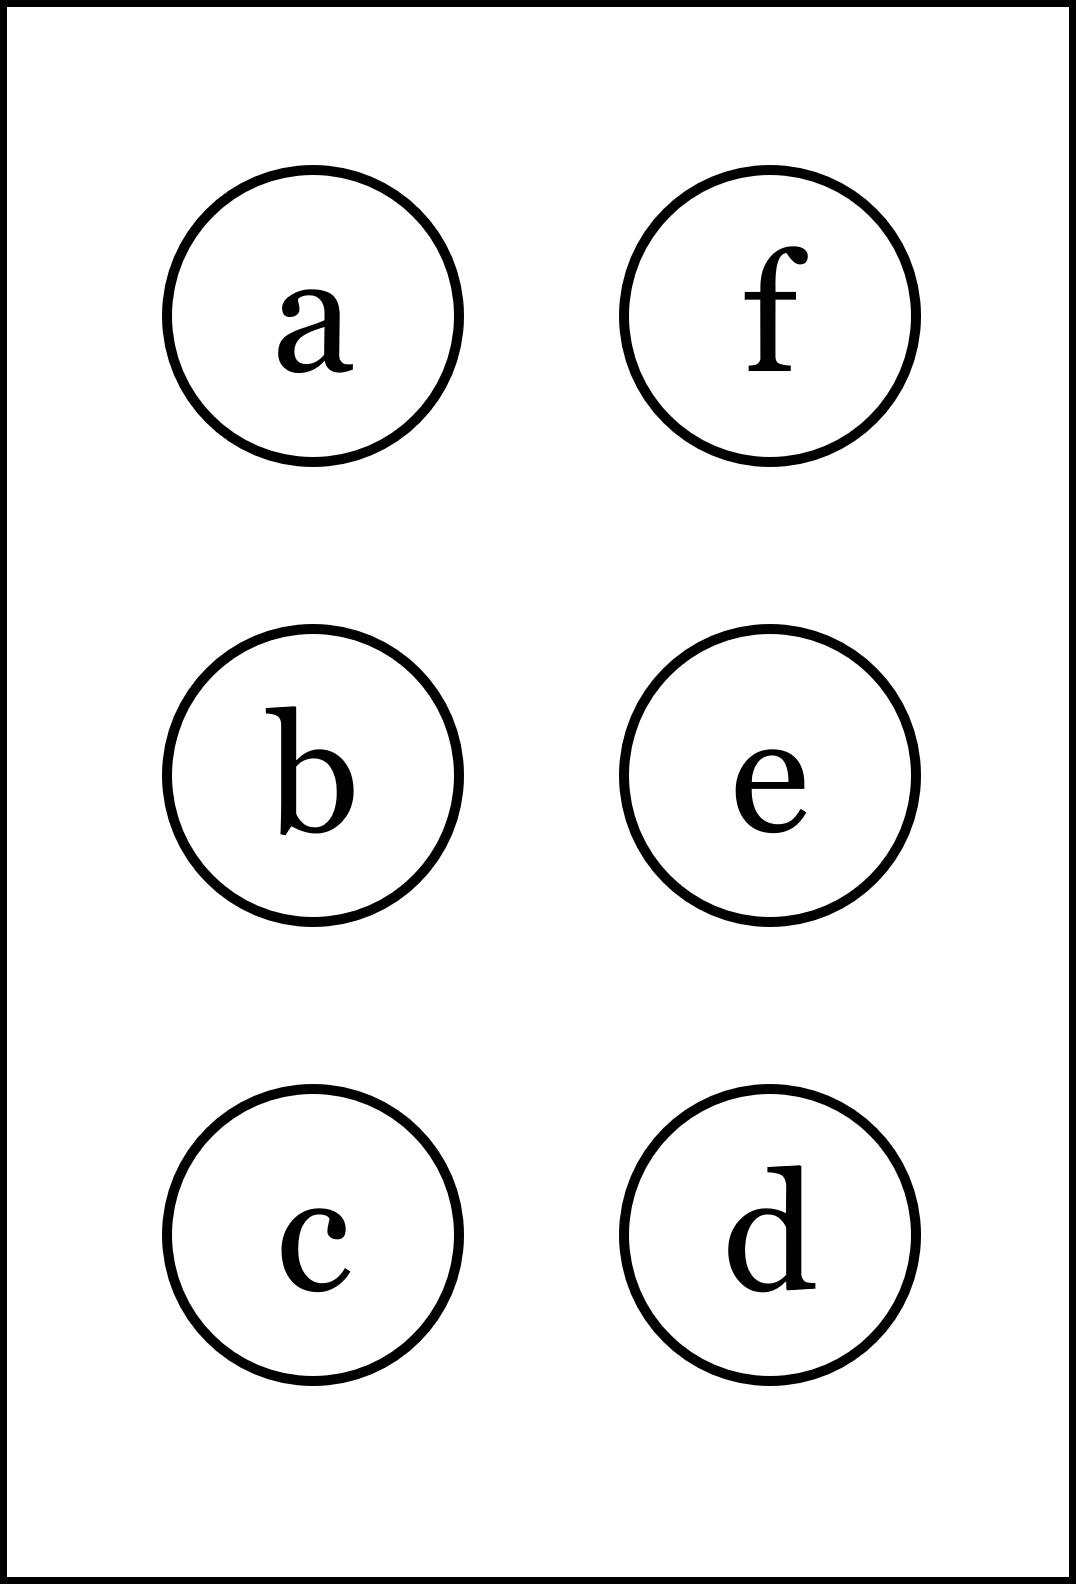
\includegraphics[height=40mm]{../images/braille.png}
{\small Písmeno Braillovej abecedy}
\end{center}
\end{minipage}
\end{center}
\end{minipage}
%
\end{tabular}
\newpage
\thispagestyle{empty}
\begin{tabular}{c:c}
\begin{minipage}[c][104.5mm][t]{0.5\linewidth}
\begin{center}
\vspace{7mm}
{\huge Kubická rovnice, skupina \textit{Eta $\eta$} -\romannumeral1}\\[5mm]
\textit{Jméno:}\phantom{xxxxxxxxxxxxxxxxxxxxxxxxxxxxxxxxxxxxxxxxxxxxxxxxxxxxxxxxxxxxxxxxx}\\[5mm]
\begin{minipage}{0.95\linewidth}
\begin{center}
\textbf{Vypočítej součet kořenů kubické rovnice.} Dvojitý kořen považuj do součtu za dva,\\trojitý kořen za tři. Pokud ti vyjde stejný výsledek jako je za otazníky, tak napravo\\barvi příslušející kroužek načerno. \textbf{Spolu odevzdejte výsledné slovo}.
\end{center}
\end{minipage}
\\[1mm]
\begin{minipage}{0.79\linewidth}
\begin{center}
\begin{varwidth}{\linewidth}
\begin{enumerate}
\Large
\item $5x^3+25x^2+30x=0$\quad \dotfill\; ???\;\dotfill \quad $-5$
\item $x^3-9x^2+15x-7=0$\quad \dotfill\; ???\;\dotfill \quad $9$
\item $4x^3+26x^2+46x+24=0$\quad \dotfill\; ???\;\dotfill \quad $\nicefrac{-7}{2}$
\item $-7x^3-50x^2-49x-6=0$\quad \dotfill\; ???\;\dotfill \quad $\nicefrac{-48}{7}$
\item \quad \dotfill\; ???\;\dotfill \quad vybarvi
\item \quad \dotfill\; ???\;\dotfill \quad nebarvi
\end{enumerate}
\end{varwidth}
\end{center}
\end{minipage}
\begin{minipage}{0.20\linewidth}
\begin{center}
{\Huge\bfseries 1.} \\[2mm]
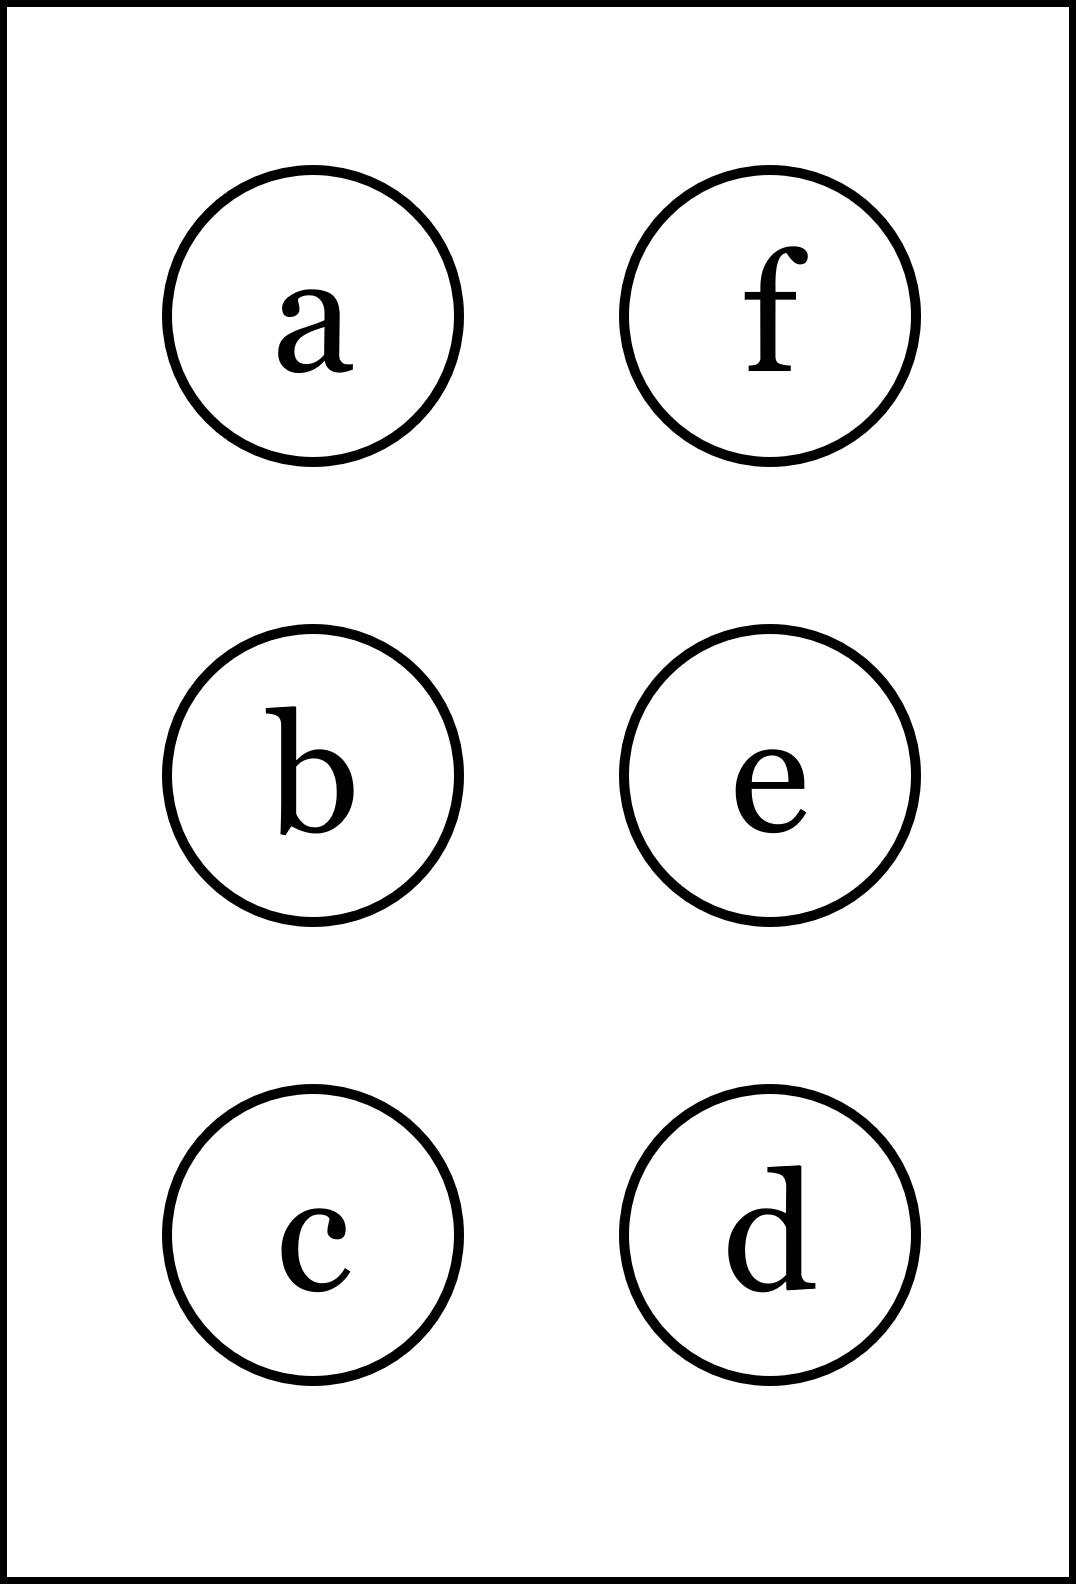
\includegraphics[height=40mm]{../images/braille.png}
{\small Písmeno Braillovej abecedy}
\end{center}
\end{minipage}
\end{center}
\end{minipage}
&
\begin{minipage}[c][104.5mm][t]{0.5\linewidth}
\begin{center}
\vspace{7mm}
{\huge Kubická rovnice, skupina \textit{Eta $\eta$} -\romannumeral2}\\[5mm]
\textit{Jméno:}\phantom{xxxxxxxxxxxxxxxxxxxxxxxxxxxxxxxxxxxxxxxxxxxxxxxxxxxxxxxxxxxxxxxxx}\\[5mm]
\begin{minipage}{0.95\linewidth}
\begin{center}
\textbf{Vypočítej součet kořenů kubické rovnice.} Dvojitý kořen považuj do součtu za dva,\\trojitý kořen za tři. Pokud ti vyjde stejný výsledek jako je za otazníky, tak napravo\\barvi příslušející kroužek načerno. \textbf{Spolu odevzdejte výsledné slovo}.
\end{center}
\end{minipage}
\\[1mm]
\begin{minipage}{0.79\linewidth}
\begin{center}
\begin{varwidth}{\linewidth}
\begin{enumerate}
\Large
\item $x^3+9x^2+8x=0$\quad \dotfill\; ???\;\dotfill \quad $-9$
\item $3x^3-3x^2-3x+3=0$\quad \dotfill\; ???\;\dotfill \quad $-1$
\item $-9x^3-9x^2+40x+28=0$\quad \dotfill\; ???\;\dotfill \quad $\nicefrac{11}{3}$
\item $-4x^3+17x^2+71x+42=0$\quad \dotfill\; ???\;\dotfill \quad $\nicefrac{33}{4}$
\item \quad \dotfill\; ???\;\dotfill \quad nebarvi
\item \quad \dotfill\; ???\;\dotfill \quad nebarvi
\end{enumerate}
\end{varwidth}
\end{center}
\end{minipage}
\begin{minipage}{0.20\linewidth}
\begin{center}
{\Huge\bfseries 2.} \\[2mm]
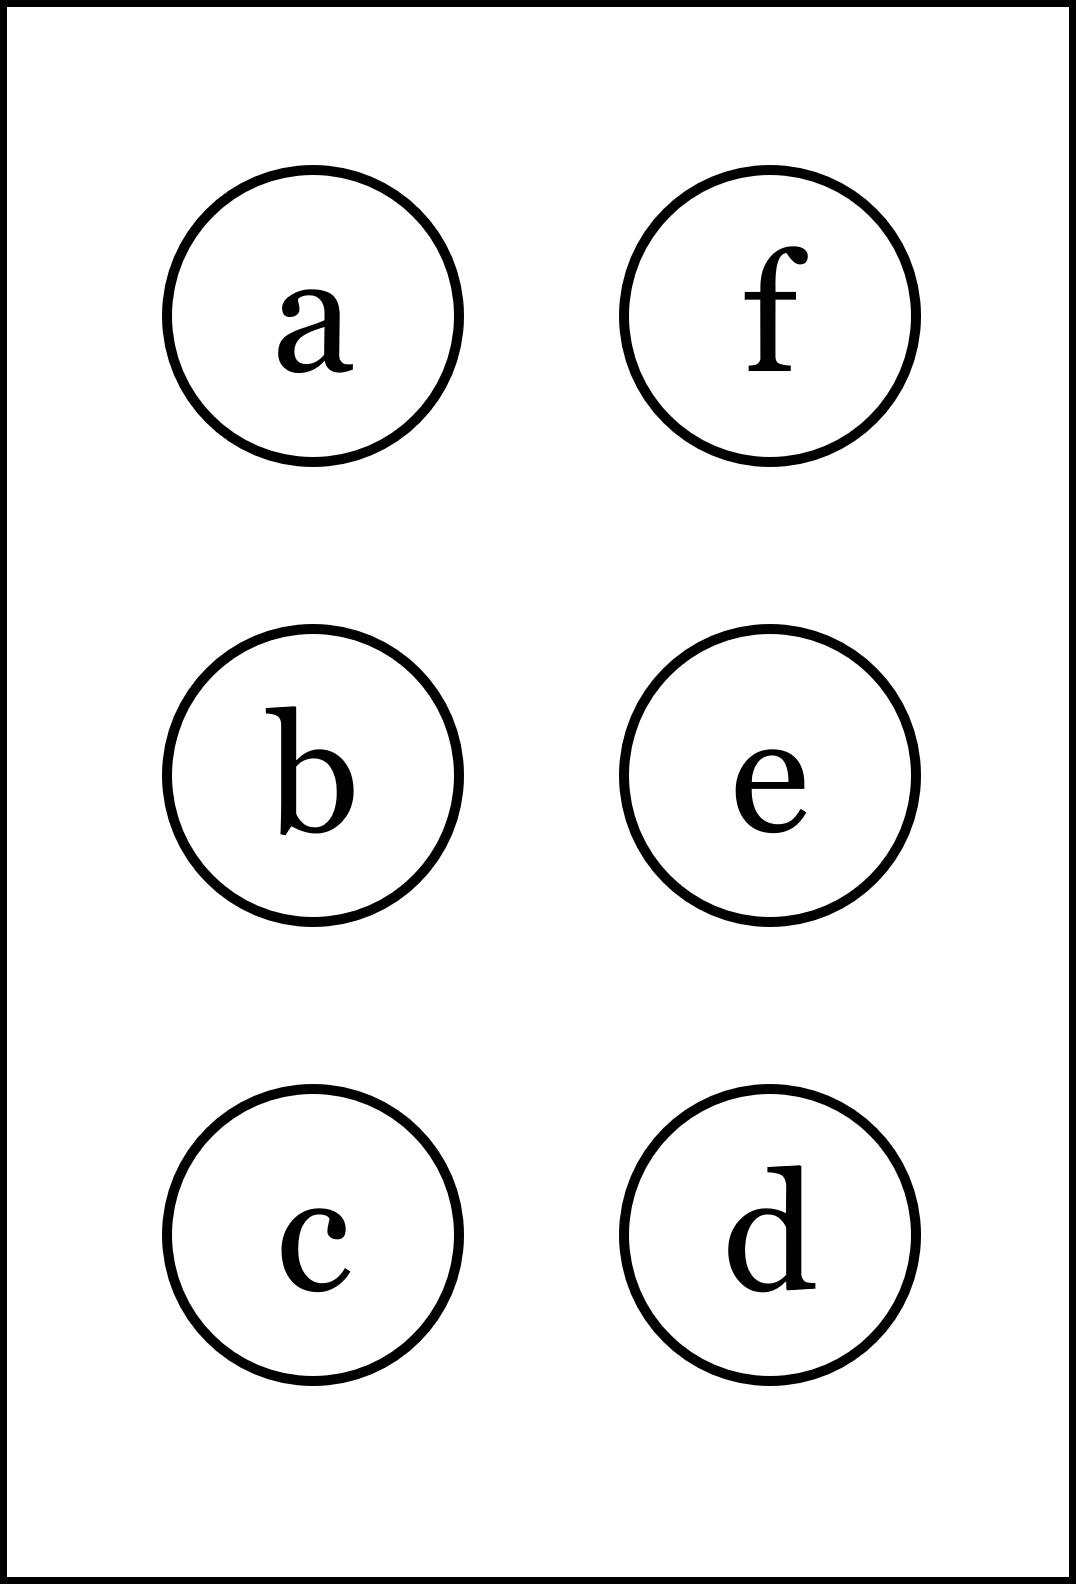
\includegraphics[height=40mm]{../images/braille.png}
{\small Písmeno Braillovej abecedy}
\end{center}
\end{minipage}
\end{center}
\end{minipage}
\\ \hdashline
\begin{minipage}[c][104.5mm][t]{0.5\linewidth}
\begin{center}
\vspace{7mm}
{\huge Kubická rovnice, skupina \textit{Eta $\eta$} -\romannumeral3}\\[5mm]
\textit{Jméno:}\phantom{xxxxxxxxxxxxxxxxxxxxxxxxxxxxxxxxxxxxxxxxxxxxxxxxxxxxxxxxxxxxxxxxx}\\[5mm]
\begin{minipage}{0.95\linewidth}
\begin{center}
\textbf{Vypočítej součet kořenů kubické rovnice.} Dvojitý kořen považuj do součtu za dva,\\trojitý kořen za tři. Pokud ti vyjde stejný výsledek jako je za otazníky, tak napravo\\barvi příslušející kroužek načerno. \textbf{Spolu odevzdejte výsledné slovo}.
\end{center}
\end{minipage}
\\[1mm]
\begin{minipage}{0.79\linewidth}
\begin{center}
\begin{varwidth}{\linewidth}
\begin{enumerate}
\Large
\item $6x^3+18x^2-24x=0$\quad \dotfill\; ???\;\dotfill \quad $-3$
\item $-2x^3-2x^2+20x-16=0$\quad \dotfill\; ???\;\dotfill \quad $7$
\item $-12x^3+36x^2+12x-36=0$\quad \dotfill\; ???\;\dotfill \quad $3$
\item $5x^3+7x^2-x-3=0$\quad \dotfill\; ???\;\dotfill \quad $\nicefrac{-13}{5}$
\item \quad \dotfill\; ???\;\dotfill \quad vybarvi
\item \quad \dotfill\; ???\;\dotfill \quad vybarvi
\end{enumerate}
\end{varwidth}
\end{center}
\end{minipage}
\begin{minipage}{0.20\linewidth}
\begin{center}
{\Huge\bfseries 3.} \\[2mm]
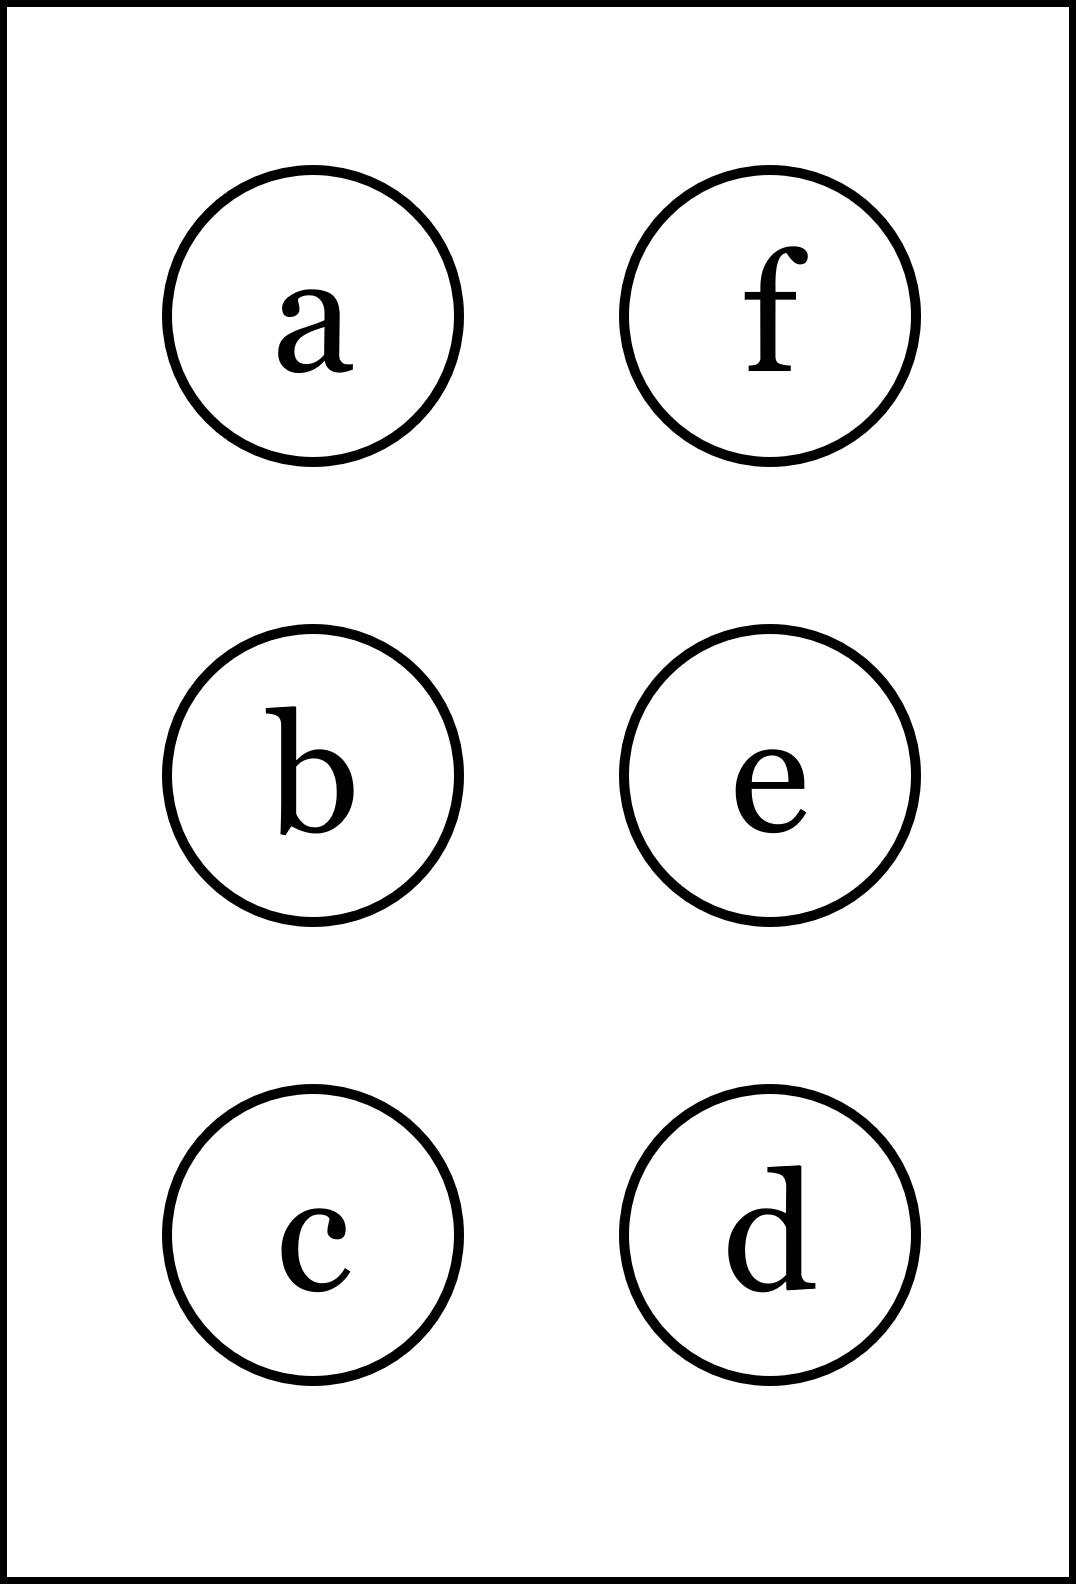
\includegraphics[height=40mm]{../images/braille.png}
{\small Písmeno Braillovej abecedy}
\end{center}
\end{minipage}
\end{center}
\end{minipage}
&
\begin{minipage}[c][104.5mm][t]{0.5\linewidth}
\begin{center}
\vspace{7mm}
{\huge Kubická rovnice, skupina \textit{Eta $\eta$} -\romannumeral4}\\[5mm]
\textit{Jméno:}\phantom{xxxxxxxxxxxxxxxxxxxxxxxxxxxxxxxxxxxxxxxxxxxxxxxxxxxxxxxxxxxxxxxxx}\\[5mm]
\begin{minipage}{0.95\linewidth}
\begin{center}
\textbf{Vypočítej součet kořenů kubické rovnice.} Dvojitý kořen považuj do součtu za dva,\\trojitý kořen za tři. Pokud ti vyjde stejný výsledek jako je za otazníky, tak napravo\\barvi příslušející kroužek načerno. \textbf{Spolu odevzdejte výsledné slovo}.
\end{center}
\end{minipage}
\\[1mm]
\begin{minipage}{0.79\linewidth}
\begin{center}
\begin{varwidth}{\linewidth}
\begin{enumerate}
\Large
\item $x^3+6x^2-7x=0$\quad \dotfill\; ???\;\dotfill \quad $-6$
\item $-2x^3+8x^2+2x-8=0$\quad \dotfill\; ???\;\dotfill \quad $-4$
\item $18x^3+45x^2+9x-18=0$\quad \dotfill\; ???\;\dotfill \quad $\nicefrac{-7}{2}$
\item $-2x^3-18x^2-48x-32=0$\quad \dotfill\; ???\;\dotfill \quad $-1$
\item \quad \dotfill\; ???\;\dotfill \quad nebarvi
\item \quad \dotfill\; ???\;\dotfill \quad nebarvi
\end{enumerate}
\end{varwidth}
\end{center}
\end{minipage}
\begin{minipage}{0.20\linewidth}
\begin{center}
{\Huge\bfseries 4.} \\[2mm]
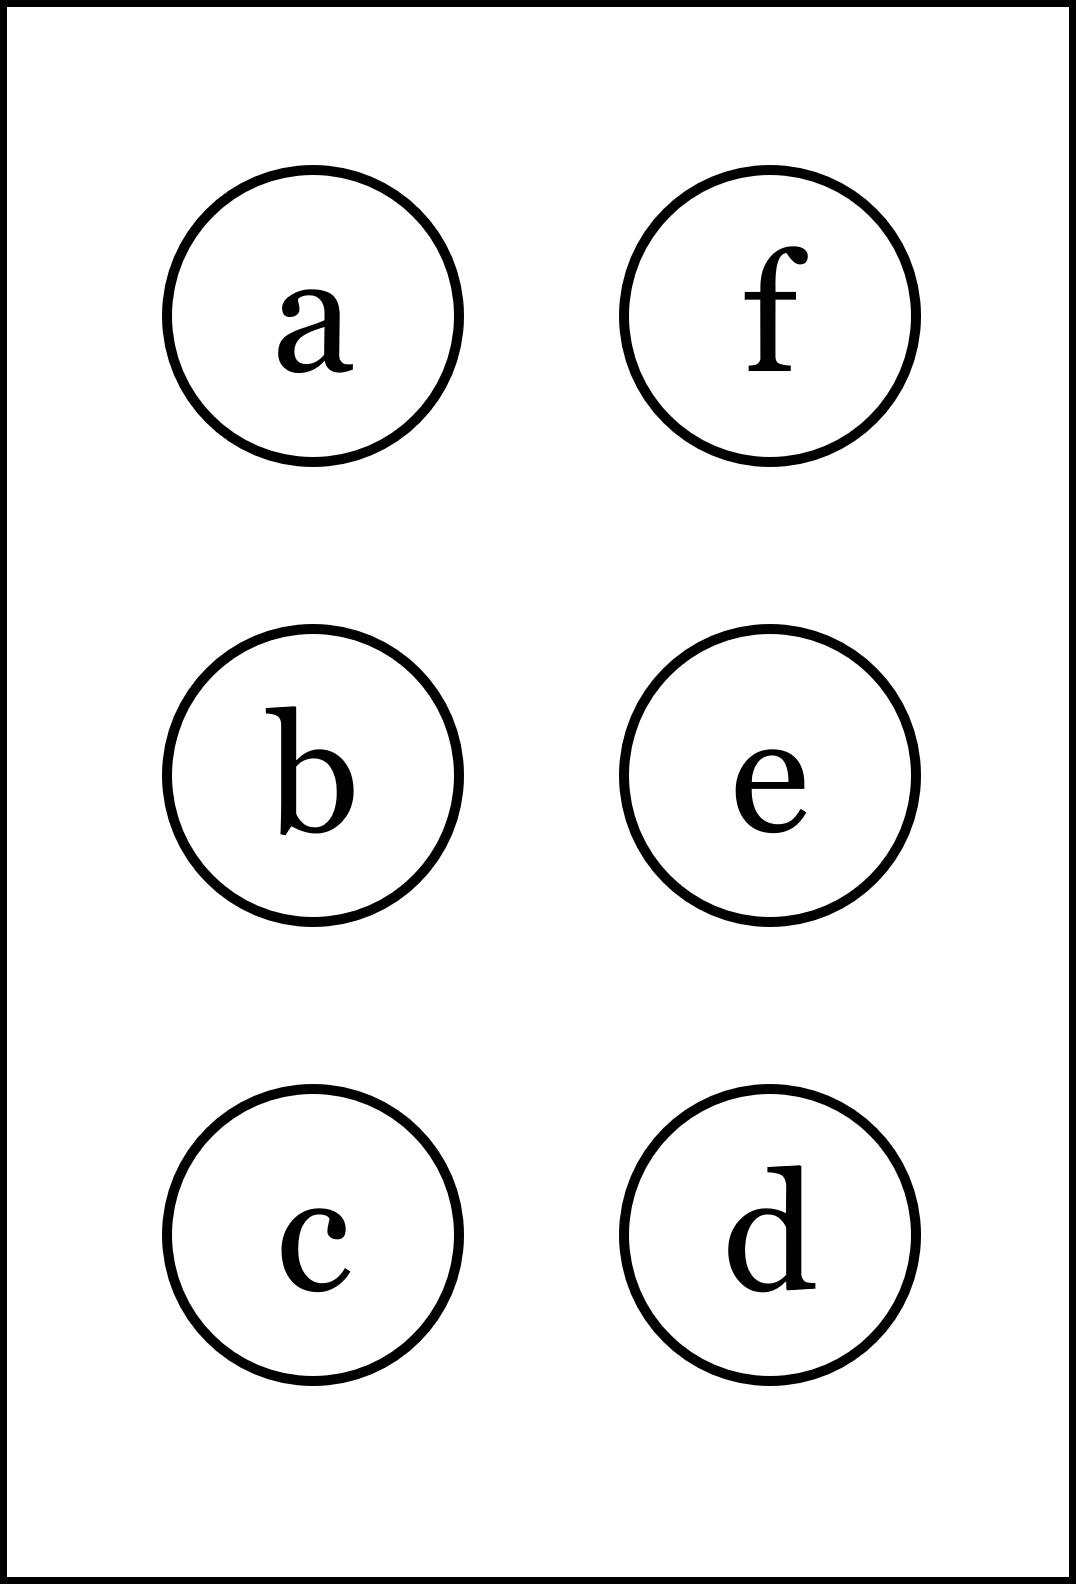
\includegraphics[height=40mm]{../images/braille.png}
{\small Písmeno Braillovej abecedy}
\end{center}
\end{minipage}
\end{center}
\end{minipage}
%
\end{tabular}
\newpage
\thispagestyle{empty}
\begin{tabular}{c:c}
\begin{minipage}[c][104.5mm][t]{0.5\linewidth}
\begin{center}
\vspace{7mm}
{\huge Kubická rovnice, skupina \textit{Theta $\theta$} -\romannumeral1}\\[5mm]
\textit{Jméno:}\phantom{xxxxxxxxxxxxxxxxxxxxxxxxxxxxxxxxxxxxxxxxxxxxxxxxxxxxxxxxxxxxxxxxx}\\[5mm]
\begin{minipage}{0.95\linewidth}
\begin{center}
\textbf{Vypočítej součet kořenů kubické rovnice.} Dvojitý kořen považuj do součtu za dva,\\trojitý kořen za tři. Pokud ti vyjde stejný výsledek jako je za otazníky, tak napravo\\barvi příslušející kroužek načerno. \textbf{Spolu odevzdejte výsledné slovo}.
\end{center}
\end{minipage}
\\[1mm]
\begin{minipage}{0.79\linewidth}
\begin{center}
\begin{varwidth}{\linewidth}
\begin{enumerate}
\Large
\item $-6x^3-18x^2-12x=0$\quad \dotfill\; ???\;\dotfill \quad $1$
\item $2x^3-8x^2-14x+20=0$\quad \dotfill\; ???\;\dotfill \quad $4$
\item $-6x^3+18x^2-24=0$\quad \dotfill\; ???\;\dotfill \quad $-1$
\item $-4x^3-12x^2+36x-20=0$\quad \dotfill\; ???\;\dotfill \quad $-5$
\item \quad \dotfill\; ???\;\dotfill \quad vybarvi
\item \quad \dotfill\; ???\;\dotfill \quad vybarvi
\end{enumerate}
\end{varwidth}
\end{center}
\end{minipage}
\begin{minipage}{0.20\linewidth}
\begin{center}
{\Huge\bfseries 1.} \\[2mm]
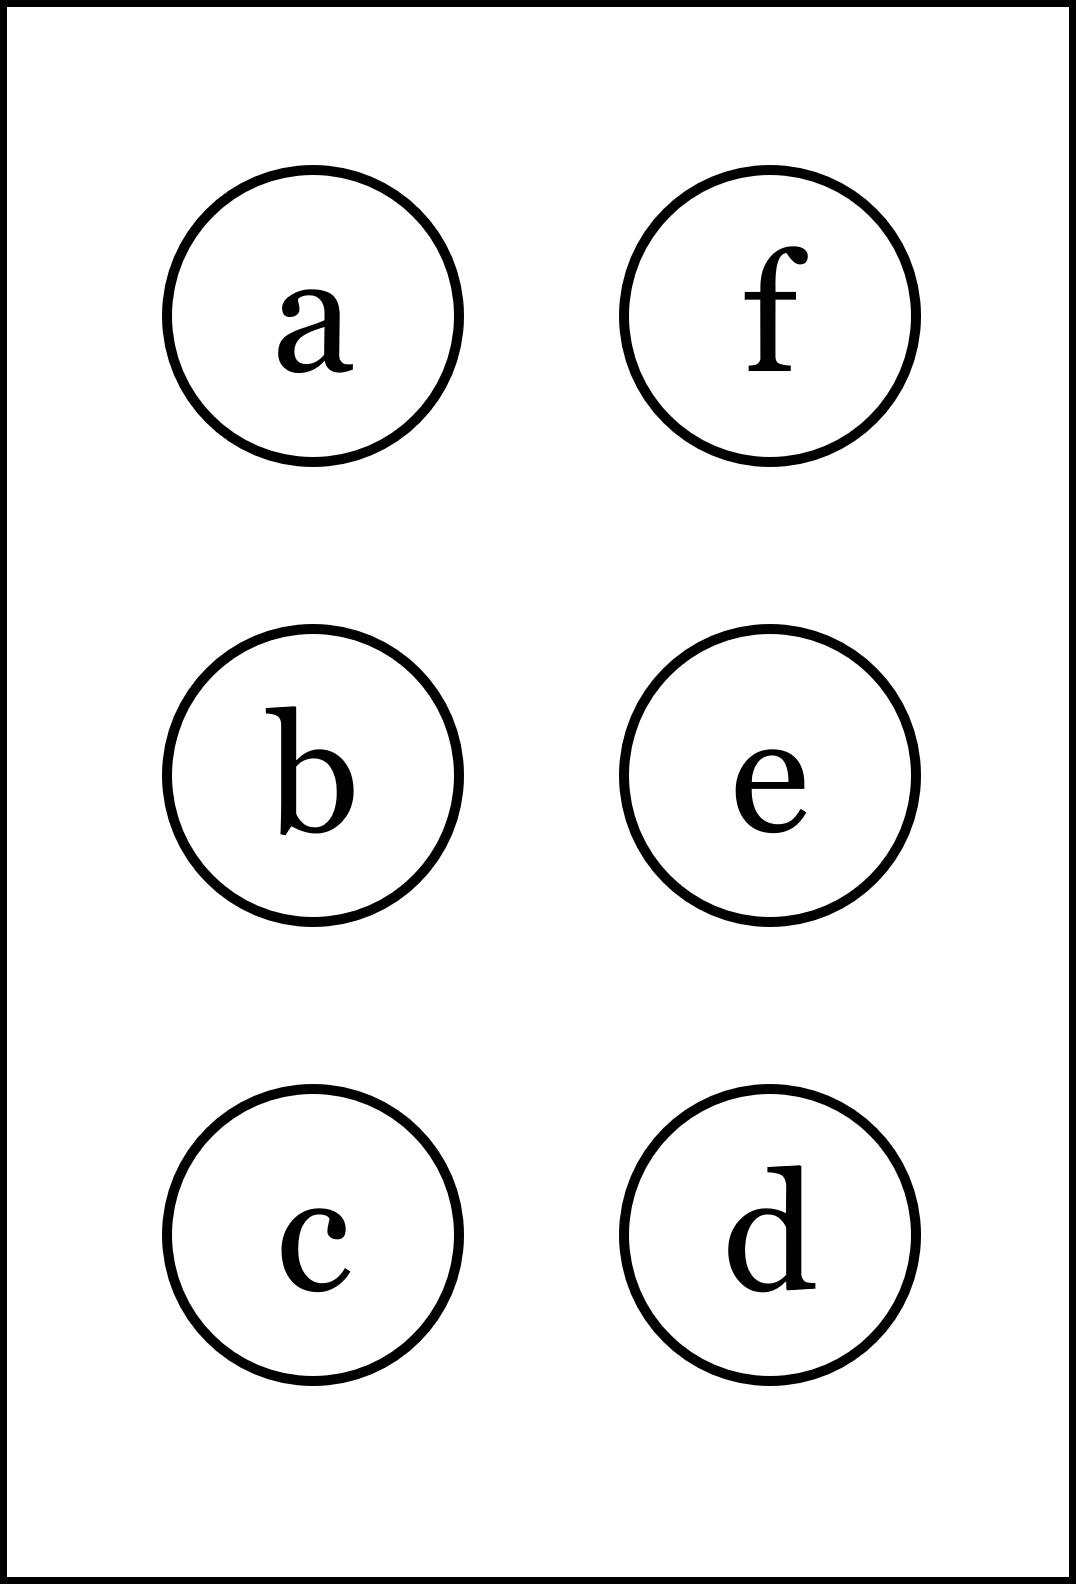
\includegraphics[height=40mm]{../images/braille.png}
{\small Písmeno Braillovej abecedy}
\end{center}
\end{minipage}
\end{center}
\end{minipage}
&
\begin{minipage}[c][104.5mm][t]{0.5\linewidth}
\begin{center}
\vspace{7mm}
{\huge Kubická rovnice, skupina \textit{Theta $\theta$} -\romannumeral2}\\[5mm]
\textit{Jméno:}\phantom{xxxxxxxxxxxxxxxxxxxxxxxxxxxxxxxxxxxxxxxxxxxxxxxxxxxxxxxxxxxxxxxxx}\\[5mm]
\begin{minipage}{0.95\linewidth}
\begin{center}
\textbf{Vypočítej součet kořenů kubické rovnice.} Dvojitý kořen považuj do součtu za dva,\\trojitý kořen za tři. Pokud ti vyjde stejný výsledek jako je za otazníky, tak napravo\\barvi příslušející kroužek načerno. \textbf{Spolu odevzdejte výsledné slovo}.
\end{center}
\end{minipage}
\\[1mm]
\begin{minipage}{0.79\linewidth}
\begin{center}
\begin{varwidth}{\linewidth}
\begin{enumerate}
\Large
\item $4x^3+16x^2+12x=0$\quad \dotfill\; ???\;\dotfill \quad $-4$
\item $3x^3+3x^2-15x+9=0$\quad \dotfill\; ???\;\dotfill \quad $5$
\item $-2x^3-16x^2-18x+36=0$\quad \dotfill\; ???\;\dotfill \quad $-10$
\item $-7x^3-37x^2+32x+12=0$\quad \dotfill\; ???\;\dotfill \quad $\nicefrac{-33}{7}$
\item \quad \dotfill\; ???\;\dotfill \quad nebarvi
\item \quad \dotfill\; ???\;\dotfill \quad nebarvi
\end{enumerate}
\end{varwidth}
\end{center}
\end{minipage}
\begin{minipage}{0.20\linewidth}
\begin{center}
{\Huge\bfseries 2.} \\[2mm]
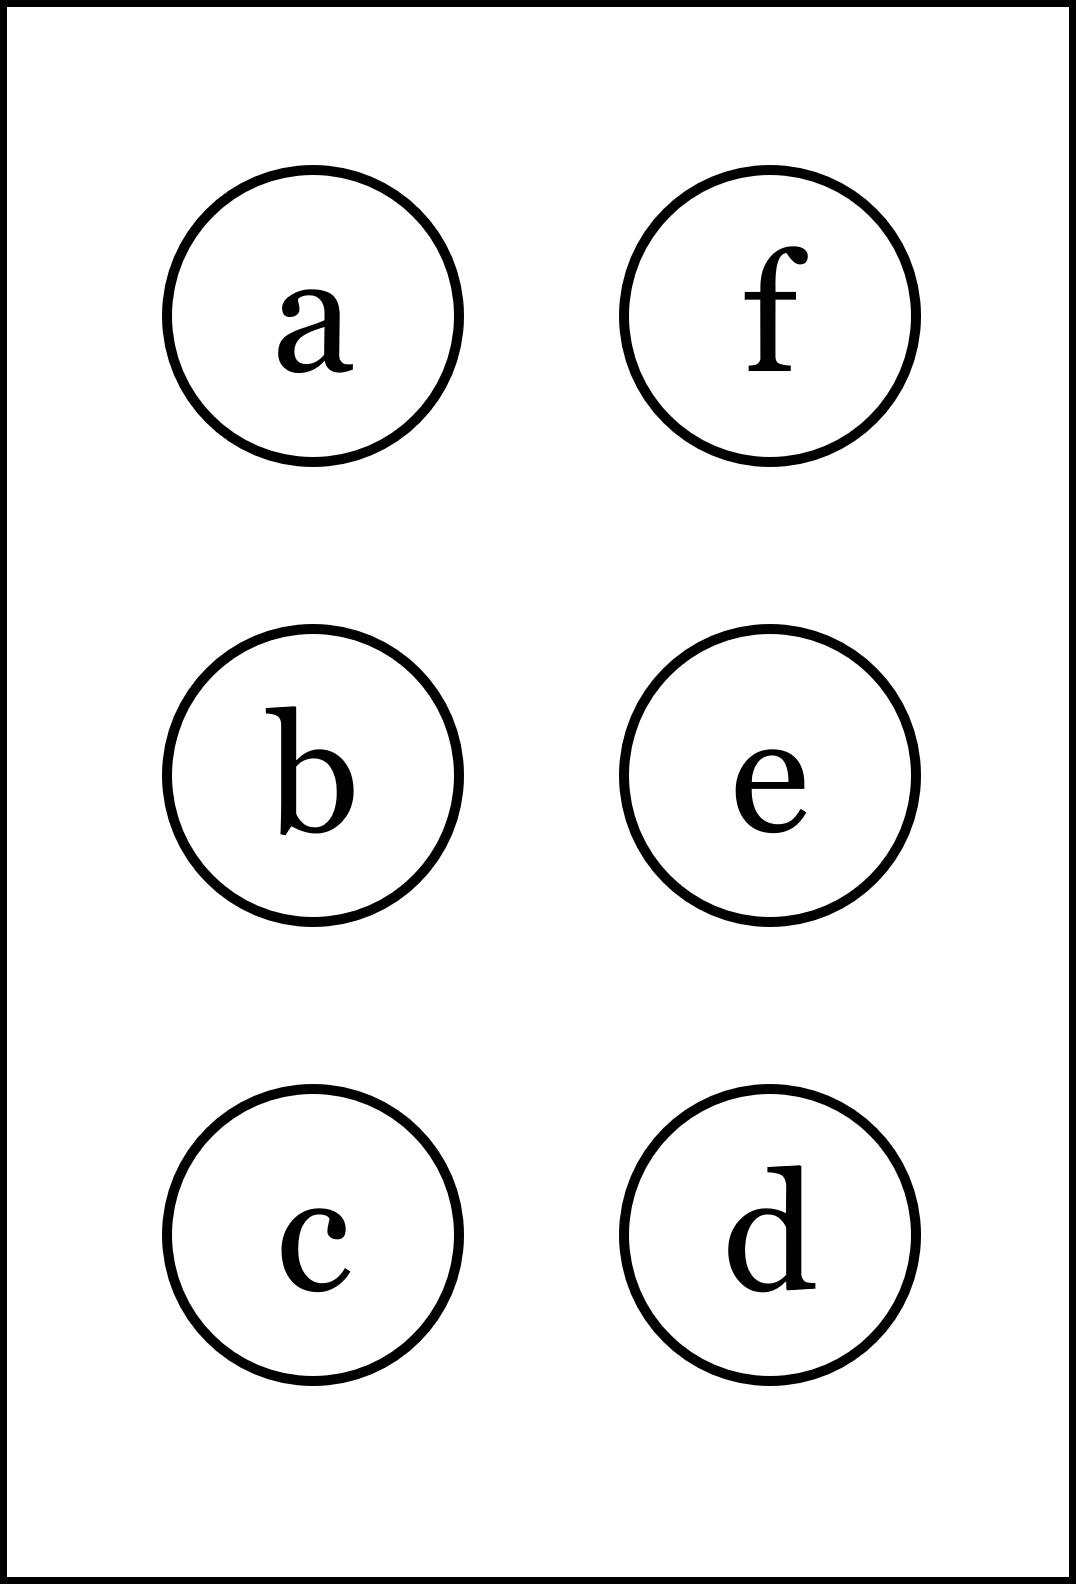
\includegraphics[height=40mm]{../images/braille.png}
{\small Písmeno Braillovej abecedy}
\end{center}
\end{minipage}
\end{center}
\end{minipage}
\\ \hdashline
\begin{minipage}[c][104.5mm][t]{0.5\linewidth}
\begin{center}
\vspace{7mm}
{\huge Kubická rovnice, skupina \textit{Theta $\theta$} -\romannumeral3}\\[5mm]
\textit{Jméno:}\phantom{xxxxxxxxxxxxxxxxxxxxxxxxxxxxxxxxxxxxxxxxxxxxxxxxxxxxxxxxxxxxxxxxx}\\[5mm]
\begin{minipage}{0.95\linewidth}
\begin{center}
\textbf{Vypočítej součet kořenů kubické rovnice.} Dvojitý kořen považuj do součtu za dva,\\trojitý kořen za tři. Pokud ti vyjde stejný výsledek jako je za otazníky, tak napravo\\barvi příslušející kroužek načerno. \textbf{Spolu odevzdejte výsledné slovo}.
\end{center}
\end{minipage}
\\[1mm]
\begin{minipage}{0.79\linewidth}
\begin{center}
\begin{varwidth}{\linewidth}
\begin{enumerate}
\Large
\item $-3x^3+3x^2+60x=0$\quad \dotfill\; ???\;\dotfill \quad $1$
\item $-3x^3+3x^2+30x+24=0$\quad \dotfill\; ???\;\dotfill \quad $-7$
\item $10x^3-31x^2-43x+28=0$\quad \dotfill\; ???\;\dotfill \quad $\nicefrac{31}{10}$
\item $3x^3+2x^2-17x+12=0$\quad \dotfill\; ???\;\dotfill \quad $\nicefrac{16}{3}$
\item \quad \dotfill\; ???\;\dotfill \quad nebarvi
\item \quad \dotfill\; ???\;\dotfill \quad nebarvi
\end{enumerate}
\end{varwidth}
\end{center}
\end{minipage}
\begin{minipage}{0.20\linewidth}
\begin{center}
{\Huge\bfseries 3.} \\[2mm]
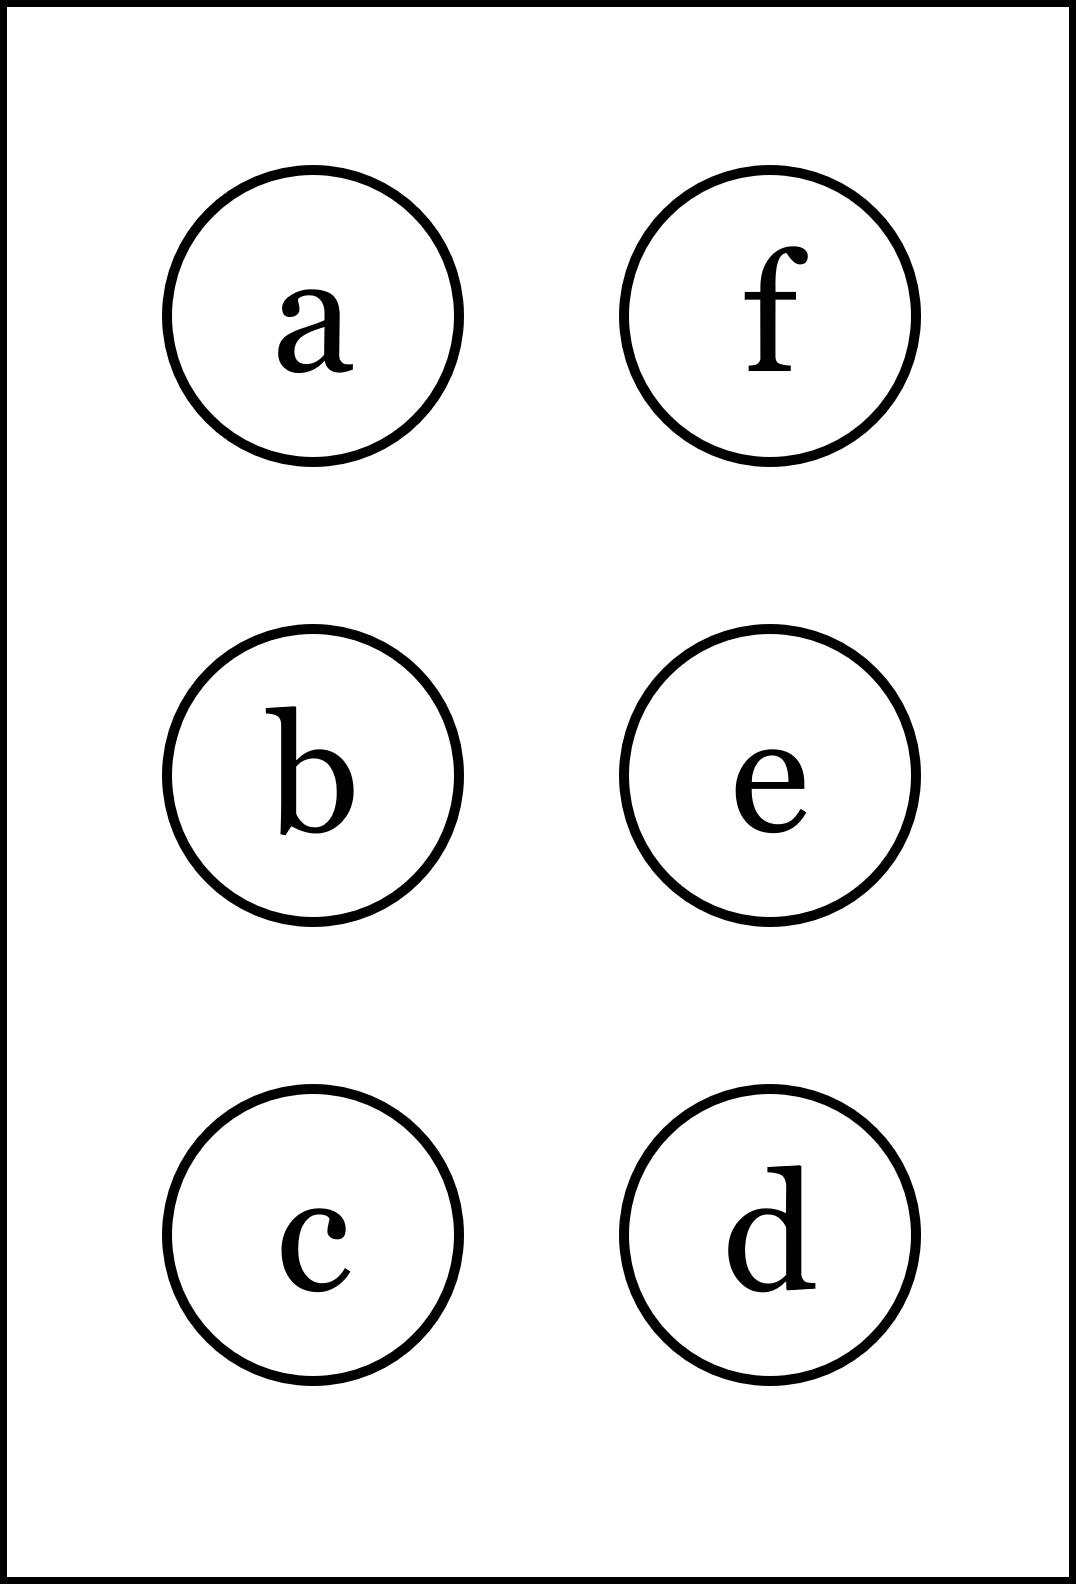
\includegraphics[height=40mm]{../images/braille.png}
{\small Písmeno Braillovej abecedy}
\end{center}
\end{minipage}
\end{center}
\end{minipage}
&
\begin{minipage}[c][104.5mm][t]{0.5\linewidth}
\begin{center}
\vspace{7mm}
{\huge Kubická rovnice, skupina \textit{Theta $\theta$} -\romannumeral4}\\[5mm]
\textit{Jméno:}\phantom{xxxxxxxxxxxxxxxxxxxxxxxxxxxxxxxxxxxxxxxxxxxxxxxxxxxxxxxxxxxxxxxxx}\\[5mm]
\begin{minipage}{0.95\linewidth}
\begin{center}
\textbf{Vypočítej součet kořenů kubické rovnice.} Dvojitý kořen považuj do součtu za dva,\\trojitý kořen za tři. Pokud ti vyjde stejný výsledek jako je za otazníky, tak napravo\\barvi příslušející kroužek načerno. \textbf{Spolu odevzdejte výsledné slovo}.
\end{center}
\end{minipage}
\\[1mm]
\begin{minipage}{0.79\linewidth}
\begin{center}
\begin{varwidth}{\linewidth}
\begin{enumerate}
\Large
\item $x^3-3x^2-10x=0$\quad \dotfill\; ???\;\dotfill \quad $3$
\item $-2x^3+16x^2-18x-36=0$\quad \dotfill\; ???\;\dotfill \quad $2$
\item $-12x^3-40x^2-36x-8=0$\quad \dotfill\; ???\;\dotfill \quad $\nicefrac{-10}{3}$
\item $18x^3-3x^2-13x-2=0$\quad \dotfill\; ???\;\dotfill \quad $\nicefrac{1}{2}$
\item \quad \dotfill\; ???\;\dotfill \quad vybarvi
\item \quad \dotfill\; ???\;\dotfill \quad nebarvi
\end{enumerate}
\end{varwidth}
\end{center}
\end{minipage}
\begin{minipage}{0.20\linewidth}
\begin{center}
{\Huge\bfseries 4.} \\[2mm]
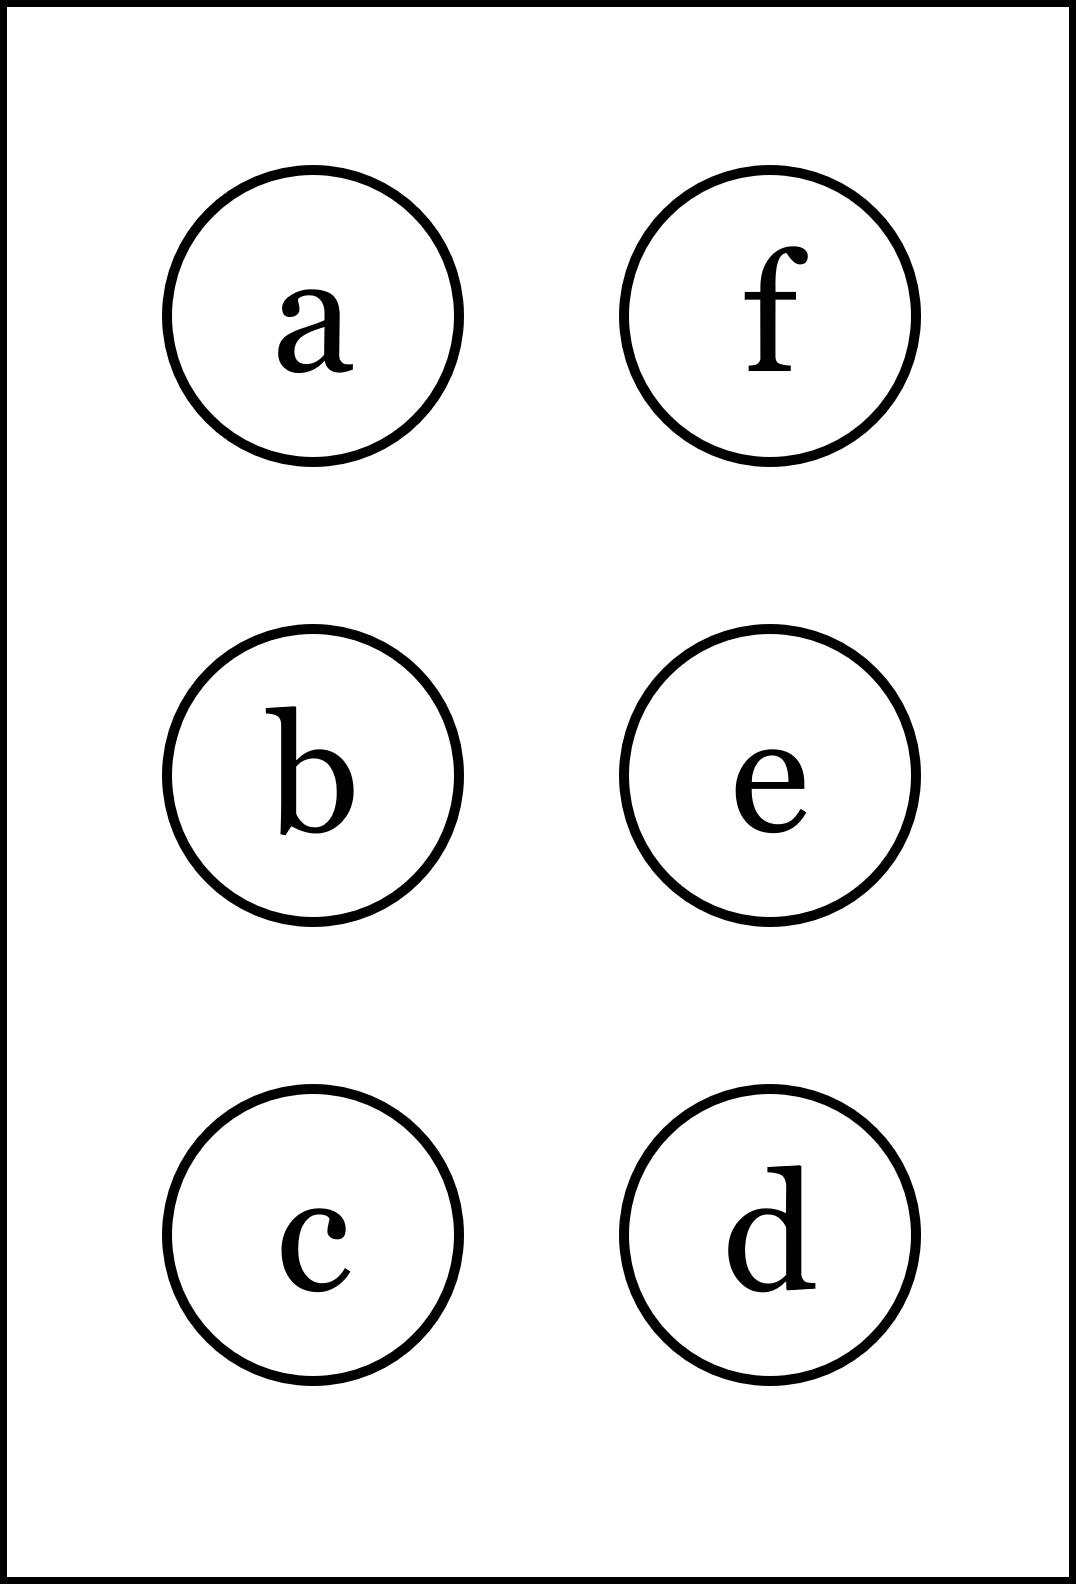
\includegraphics[height=40mm]{../images/braille.png}
{\small Písmeno Braillovej abecedy}
\end{center}
\end{minipage}
\end{center}
\end{minipage}
%
\end{tabular}
\newpage
\thispagestyle{empty}
\begin{tabular}{c:c}
\begin{minipage}[c][104.5mm][t]{0.5\linewidth}
\begin{center}
\vspace{7mm}
{\huge Kubická rovnice, skupina \textit{Iota $\iota$} -\romannumeral1}\\[5mm]
\textit{Jméno:}\phantom{xxxxxxxxxxxxxxxxxxxxxxxxxxxxxxxxxxxxxxxxxxxxxxxxxxxxxxxxxxxxxxxxx}\\[5mm]
\begin{minipage}{0.95\linewidth}
\begin{center}
\textbf{Vypočítej součet kořenů kubické rovnice.} Dvojitý kořen považuj do součtu za dva,\\trojitý kořen za tři. Pokud ti vyjde stejný výsledek jako je za otazníky, tak napravo\\barvi příslušející kroužek načerno. \textbf{Spolu odevzdejte výsledné slovo}.
\end{center}
\end{minipage}
\\[1mm]
\begin{minipage}{0.79\linewidth}
\begin{center}
\begin{varwidth}{\linewidth}
\begin{enumerate}
\Large
\item $-4x^3-4x^2+8x=0$\quad \dotfill\; ???\;\dotfill \quad $3$
\item $x^3-7x+6=0$\quad \dotfill\; ???\;\dotfill \quad $-4$
\item $-24x^3+60x^2-12x-24=0$\quad \dotfill\; ???\;\dotfill \quad $\nicefrac{5}{2}$
\item $x^3+x^2-9x-9=0$\quad \dotfill\; ???\;\dotfill \quad $-1$
\item \quad \dotfill\; ???\;\dotfill \quad nebarvi
\item \quad \dotfill\; ???\;\dotfill \quad vybarvi
\end{enumerate}
\end{varwidth}
\end{center}
\end{minipage}
\begin{minipage}{0.20\linewidth}
\begin{center}
{\Huge\bfseries 1.} \\[2mm]
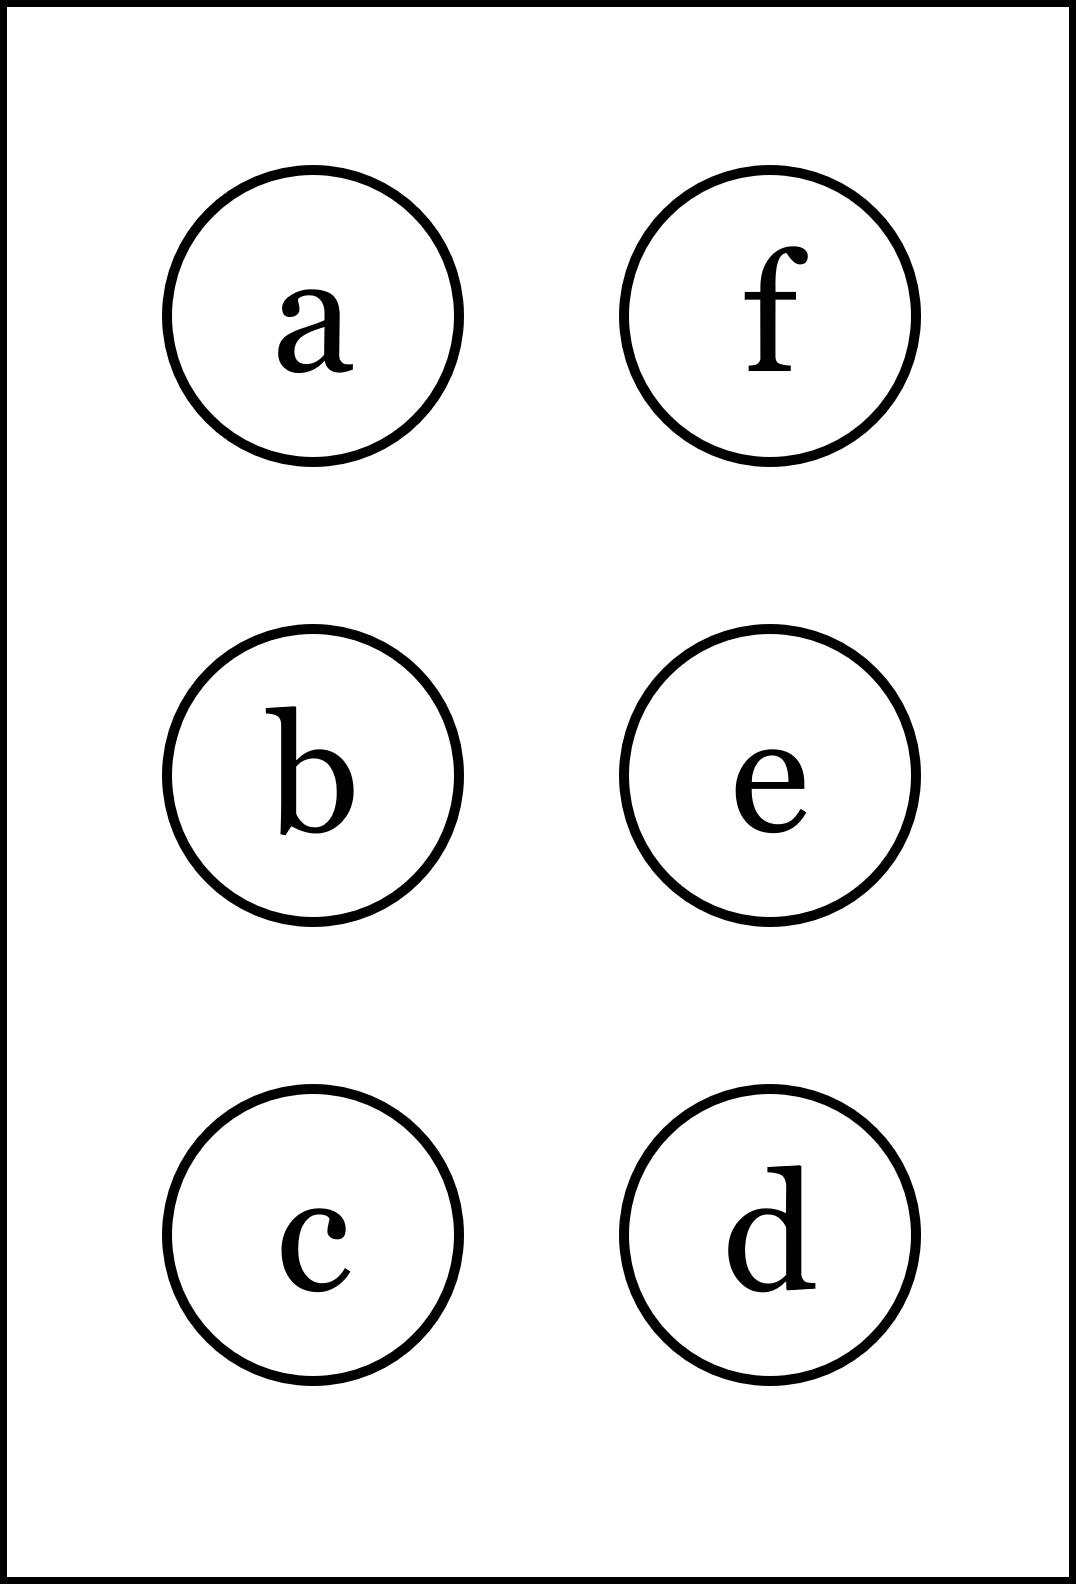
\includegraphics[height=40mm]{../images/braille.png}
{\small Písmeno Braillovej abecedy}
\end{center}
\end{minipage}
\end{center}
\end{minipage}
&
\begin{minipage}[c][104.5mm][t]{0.5\linewidth}
\begin{center}
\vspace{7mm}
{\huge Kubická rovnice, skupina \textit{Iota $\iota$} -\romannumeral2}\\[5mm]
\textit{Jméno:}\phantom{xxxxxxxxxxxxxxxxxxxxxxxxxxxxxxxxxxxxxxxxxxxxxxxxxxxxxxxxxxxxxxxxx}\\[5mm]
\begin{minipage}{0.95\linewidth}
\begin{center}
\textbf{Vypočítej součet kořenů kubické rovnice.} Dvojitý kořen považuj do součtu za dva,\\trojitý kořen za tři. Pokud ti vyjde stejný výsledek jako je za otazníky, tak napravo\\barvi příslušející kroužek načerno. \textbf{Spolu odevzdejte výsledné slovo}.
\end{center}
\end{minipage}
\\[1mm]
\begin{minipage}{0.79\linewidth}
\begin{center}
\begin{varwidth}{\linewidth}
\begin{enumerate}
\Large
\item $-2x^3+2x^2+24x=0$\quad \dotfill\; ???\;\dotfill \quad $1$
\item $-x^3+x^2+17x+15=0$\quad \dotfill\; ???\;\dotfill \quad $1$
\item $-2x^3-12x^2-22x-12=0$\quad \dotfill\; ???\;\dotfill \quad $0$
\item $12x^3-10x^2-26x+24=0$\quad \dotfill\; ???\;\dotfill \quad $\nicefrac{-11}{6}$
\item \quad \dotfill\; ???\;\dotfill \quad vybarvi
\item \quad \dotfill\; ???\;\dotfill \quad nebarvi
\end{enumerate}
\end{varwidth}
\end{center}
\end{minipage}
\begin{minipage}{0.20\linewidth}
\begin{center}
{\Huge\bfseries 2.} \\[2mm]
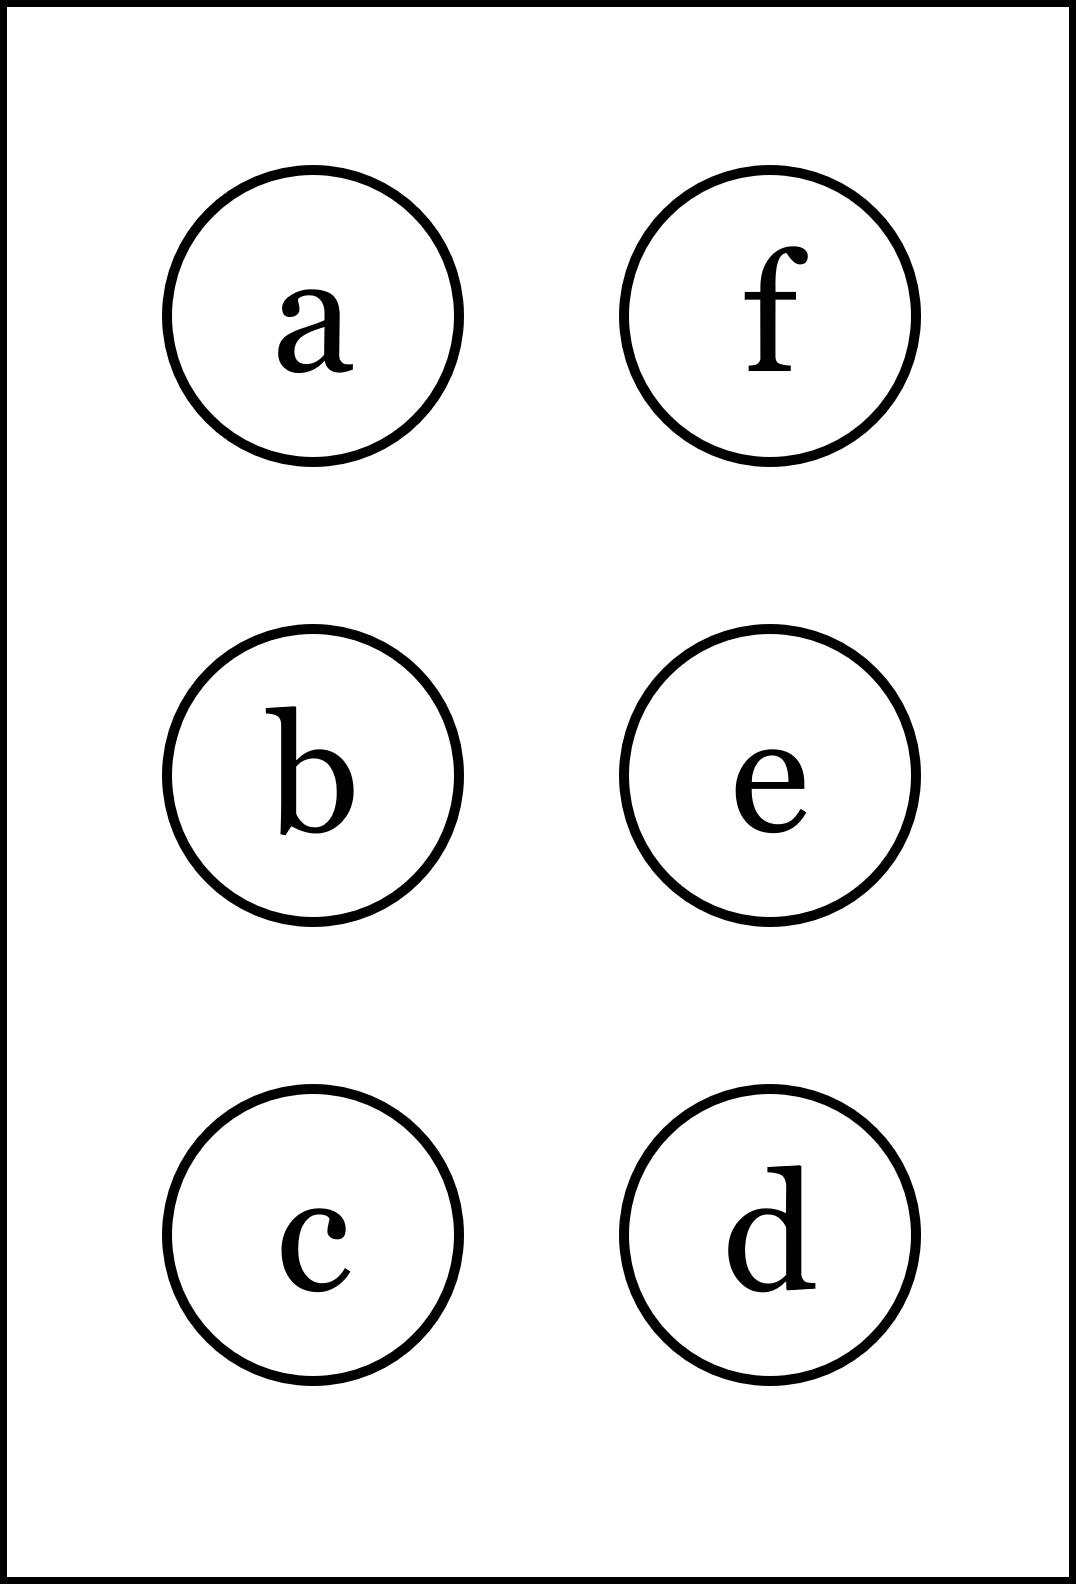
\includegraphics[height=40mm]{../images/braille.png}
{\small Písmeno Braillovej abecedy}
\end{center}
\end{minipage}
\end{center}
\end{minipage}
\\ \hdashline
\begin{minipage}[c][104.5mm][t]{0.5\linewidth}
\begin{center}
\vspace{7mm}
{\huge Kubická rovnice, skupina \textit{Iota $\iota$} -\romannumeral3}\\[5mm]
\textit{Jméno:}\phantom{xxxxxxxxxxxxxxxxxxxxxxxxxxxxxxxxxxxxxxxxxxxxxxxxxxxxxxxxxxxxxxxxx}\\[5mm]
\begin{minipage}{0.95\linewidth}
\begin{center}
\textbf{Vypočítej součet kořenů kubické rovnice.} Dvojitý kořen považuj do součtu za dva,\\trojitý kořen za tři. Pokud ti vyjde stejný výsledek jako je za otazníky, tak napravo\\barvi příslušející kroužek načerno. \textbf{Spolu odevzdejte výsledné slovo}.
\end{center}
\end{minipage}
\\[1mm]
\begin{minipage}{0.79\linewidth}
\begin{center}
\begin{varwidth}{\linewidth}
\begin{enumerate}
\Large
\item $-x^3-8x^2+9x=0$\quad \dotfill\; ???\;\dotfill \quad $-8$
\item $4x^3-20x^2+12x+36=0$\quad \dotfill\; ???\;\dotfill \quad $7$
\item $-10x^3-20x^2+10x+20=0$\quad \dotfill\; ???\;\dotfill \quad $2$
\item $15x^3+9x^2-36x+12=0$\quad \dotfill\; ???\;\dotfill \quad $\nicefrac{-7}{5}$
\item \quad \dotfill\; ???\;\dotfill \quad vybarvi
\item \quad \dotfill\; ???\;\dotfill \quad nebarvi
\end{enumerate}
\end{varwidth}
\end{center}
\end{minipage}
\begin{minipage}{0.20\linewidth}
\begin{center}
{\Huge\bfseries 3.} \\[2mm]
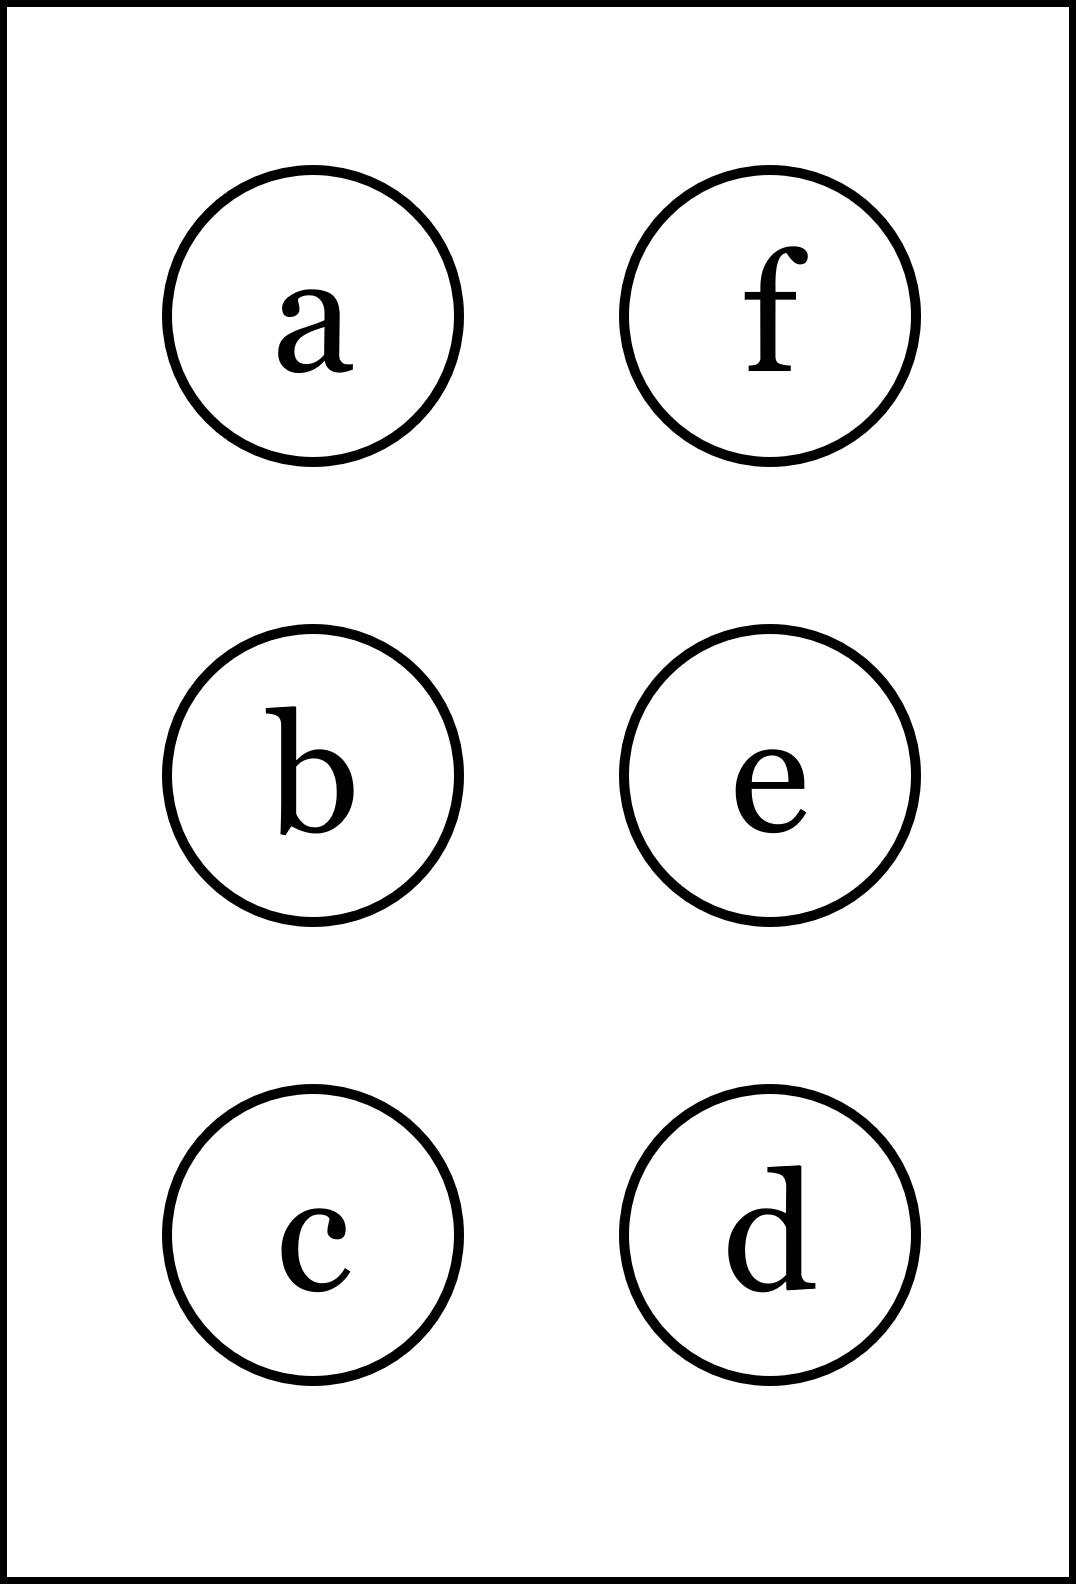
\includegraphics[height=40mm]{../images/braille.png}
{\small Písmeno Braillovej abecedy}
\end{center}
\end{minipage}
\end{center}
\end{minipage}
&
\begin{minipage}[c][104.5mm][t]{0.5\linewidth}
\begin{center}
\vspace{7mm}
{\huge Kubická rovnice, skupina \textit{Iota $\iota$} -\romannumeral4}\\[5mm]
\textit{Jméno:}\phantom{xxxxxxxxxxxxxxxxxxxxxxxxxxxxxxxxxxxxxxxxxxxxxxxxxxxxxxxxxxxxxxxxx}\\[5mm]
\begin{minipage}{0.95\linewidth}
\begin{center}
\textbf{Vypočítej součet kořenů kubické rovnice.} Dvojitý kořen považuj do součtu za dva,\\trojitý kořen za tři. Pokud ti vyjde stejný výsledek jako je za otazníky, tak napravo\\barvi příslušející kroužek načerno. \textbf{Spolu odevzdejte výsledné slovo}.
\end{center}
\end{minipage}
\\[1mm]
\begin{minipage}{0.79\linewidth}
\begin{center}
\begin{varwidth}{\linewidth}
\begin{enumerate}
\Large
\item $-x^3+x=0$\quad \dotfill\; ???\;\dotfill \quad $0$
\item $-x^3-4x^2+11x+30=0$\quad \dotfill\; ???\;\dotfill \quad $-4$
\item $x^3-x^2-22x+40=0$\quad \dotfill\; ???\;\dotfill \quad $1$
\item $-5x^3+24x^2-31x+12=0$\quad \dotfill\; ???\;\dotfill \quad $\nicefrac{16}{5}$
\item \quad \dotfill\; ???\;\dotfill \quad nebarvi
\item \quad \dotfill\; ???\;\dotfill \quad nebarvi
\end{enumerate}
\end{varwidth}
\end{center}
\end{minipage}
\begin{minipage}{0.20\linewidth}
\begin{center}
{\Huge\bfseries 4.} \\[2mm]
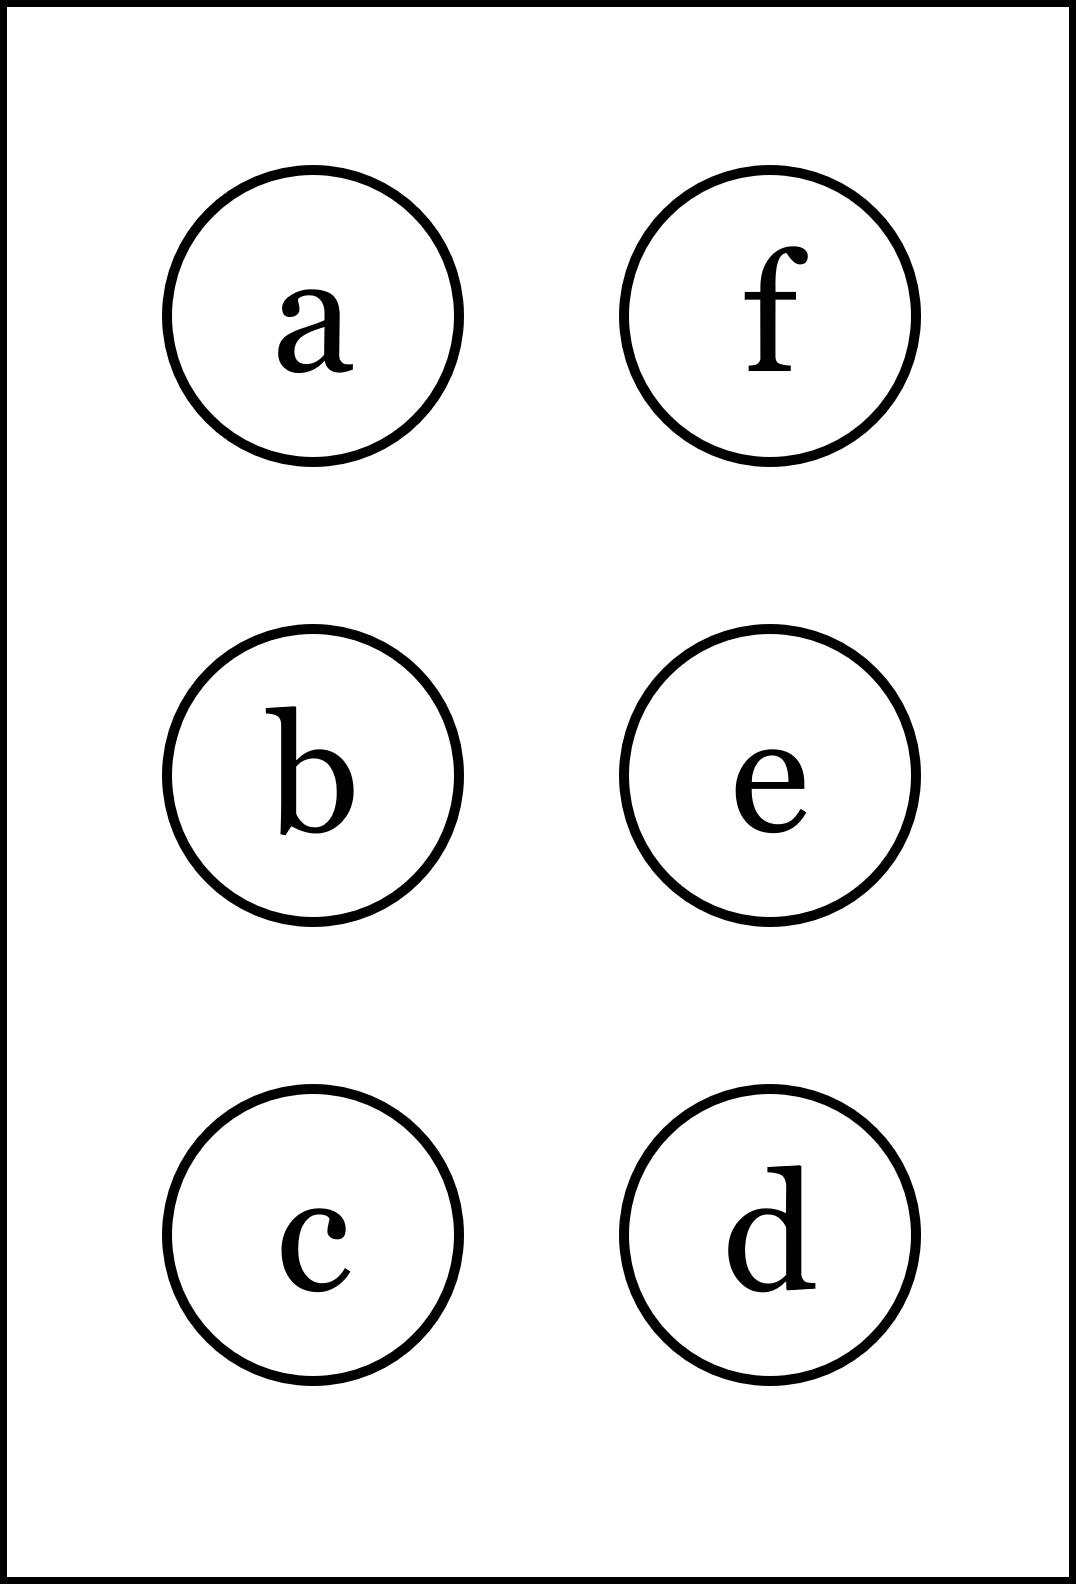
\includegraphics[height=40mm]{../images/braille.png}
{\small Písmeno Braillovej abecedy}
\end{center}
\end{minipage}
\end{center}
\end{minipage}
%
\end{tabular}
\newpage
\thispagestyle{empty}
\begin{tabular}{c:c}
\begin{minipage}[c][104.5mm][t]{0.5\linewidth}
\begin{center}
\vspace{7mm}
{\huge Kubická rovnice, skupina \textit{Kappa $\kappa$} -\romannumeral1}\\[5mm]
\textit{Jméno:}\phantom{xxxxxxxxxxxxxxxxxxxxxxxxxxxxxxxxxxxxxxxxxxxxxxxxxxxxxxxxxxxxxxxxx}\\[5mm]
\begin{minipage}{0.95\linewidth}
\begin{center}
\textbf{Vypočítej součet kořenů kubické rovnice.} Dvojitý kořen považuj do součtu za dva,\\trojitý kořen za tři. Pokud ti vyjde stejný výsledek jako je za otazníky, tak napravo\\barvi příslušející kroužek načerno. \textbf{Spolu odevzdejte výsledné slovo}.
\end{center}
\end{minipage}
\\[1mm]
\begin{minipage}{0.79\linewidth}
\begin{center}
\begin{varwidth}{\linewidth}
\begin{enumerate}
\Large
\item $-2x^3+14x^2-12x=0$\quad \dotfill\; ???\;\dotfill \quad $-5$
\item $-3x^3+24x^2-27x-54=0$\quad \dotfill\; ???\;\dotfill \quad $2$
\item $-45x^3-36x^2+45x+36=0$\quad \dotfill\; ???\;\dotfill \quad $\nicefrac{-4}{5}$
\item $12x^3+33x^2+15x-6=0$\quad \dotfill\; ???\;\dotfill \quad $\nicefrac{-11}{4}$
\item \quad \dotfill\; ???\;\dotfill \quad nebarvi
\item \quad \dotfill\; ???\;\dotfill \quad vybarvi
\end{enumerate}
\end{varwidth}
\end{center}
\end{minipage}
\begin{minipage}{0.20\linewidth}
\begin{center}
{\Huge\bfseries 1.} \\[2mm]
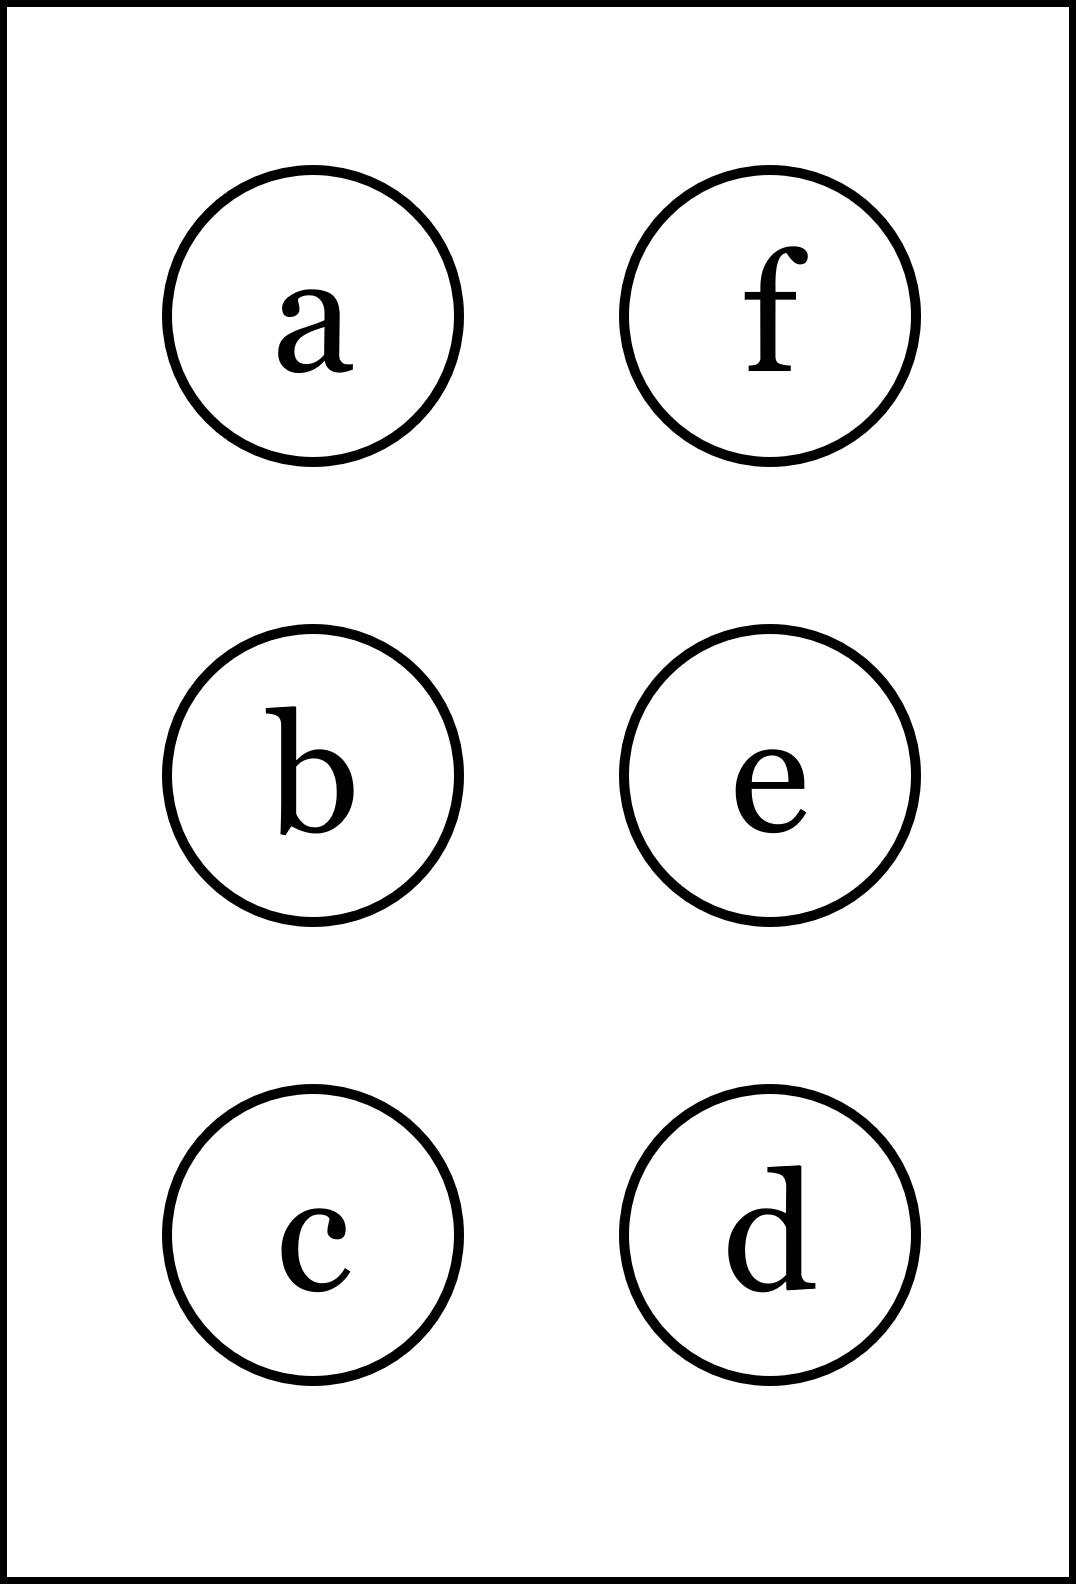
\includegraphics[height=40mm]{../images/braille.png}
{\small Písmeno Braillovej abecedy}
\end{center}
\end{minipage}
\end{center}
\end{minipage}
&
\begin{minipage}[c][104.5mm][t]{0.5\linewidth}
\begin{center}
\vspace{7mm}
{\huge Kubická rovnice, skupina \textit{Kappa $\kappa$} -\romannumeral2}\\[5mm]
\textit{Jméno:}\phantom{xxxxxxxxxxxxxxxxxxxxxxxxxxxxxxxxxxxxxxxxxxxxxxxxxxxxxxxxxxxxxxxxx}\\[5mm]
\begin{minipage}{0.95\linewidth}
\begin{center}
\textbf{Vypočítej součet kořenů kubické rovnice.} Dvojitý kořen považuj do součtu za dva,\\trojitý kořen za tři. Pokud ti vyjde stejný výsledek jako je za otazníky, tak napravo\\barvi příslušející kroužek načerno. \textbf{Spolu odevzdejte výsledné slovo}.
\end{center}
\end{minipage}
\\[1mm]
\begin{minipage}{0.79\linewidth}
\begin{center}
\begin{varwidth}{\linewidth}
\begin{enumerate}
\Large
\item $x^3+6x^2+5x=0$\quad \dotfill\; ???\;\dotfill \quad $-4$
\item $-2x^3+6x^2+12x-16=0$\quad \dotfill\; ???\;\dotfill \quad $3$
\item $16x^3+4x^2-16x-4=0$\quad \dotfill\; ???\;\dotfill \quad $\nicefrac{-1}{4}$
\item $-4x^3-2x^2+4x+2=0$\quad \dotfill\; ???\;\dotfill \quad $\nicefrac{1}{2}$
\item \quad \dotfill\; ???\;\dotfill \quad nebarvi
\item \quad \dotfill\; ???\;\dotfill \quad vybarvi
\end{enumerate}
\end{varwidth}
\end{center}
\end{minipage}
\begin{minipage}{0.20\linewidth}
\begin{center}
{\Huge\bfseries 2.} \\[2mm]
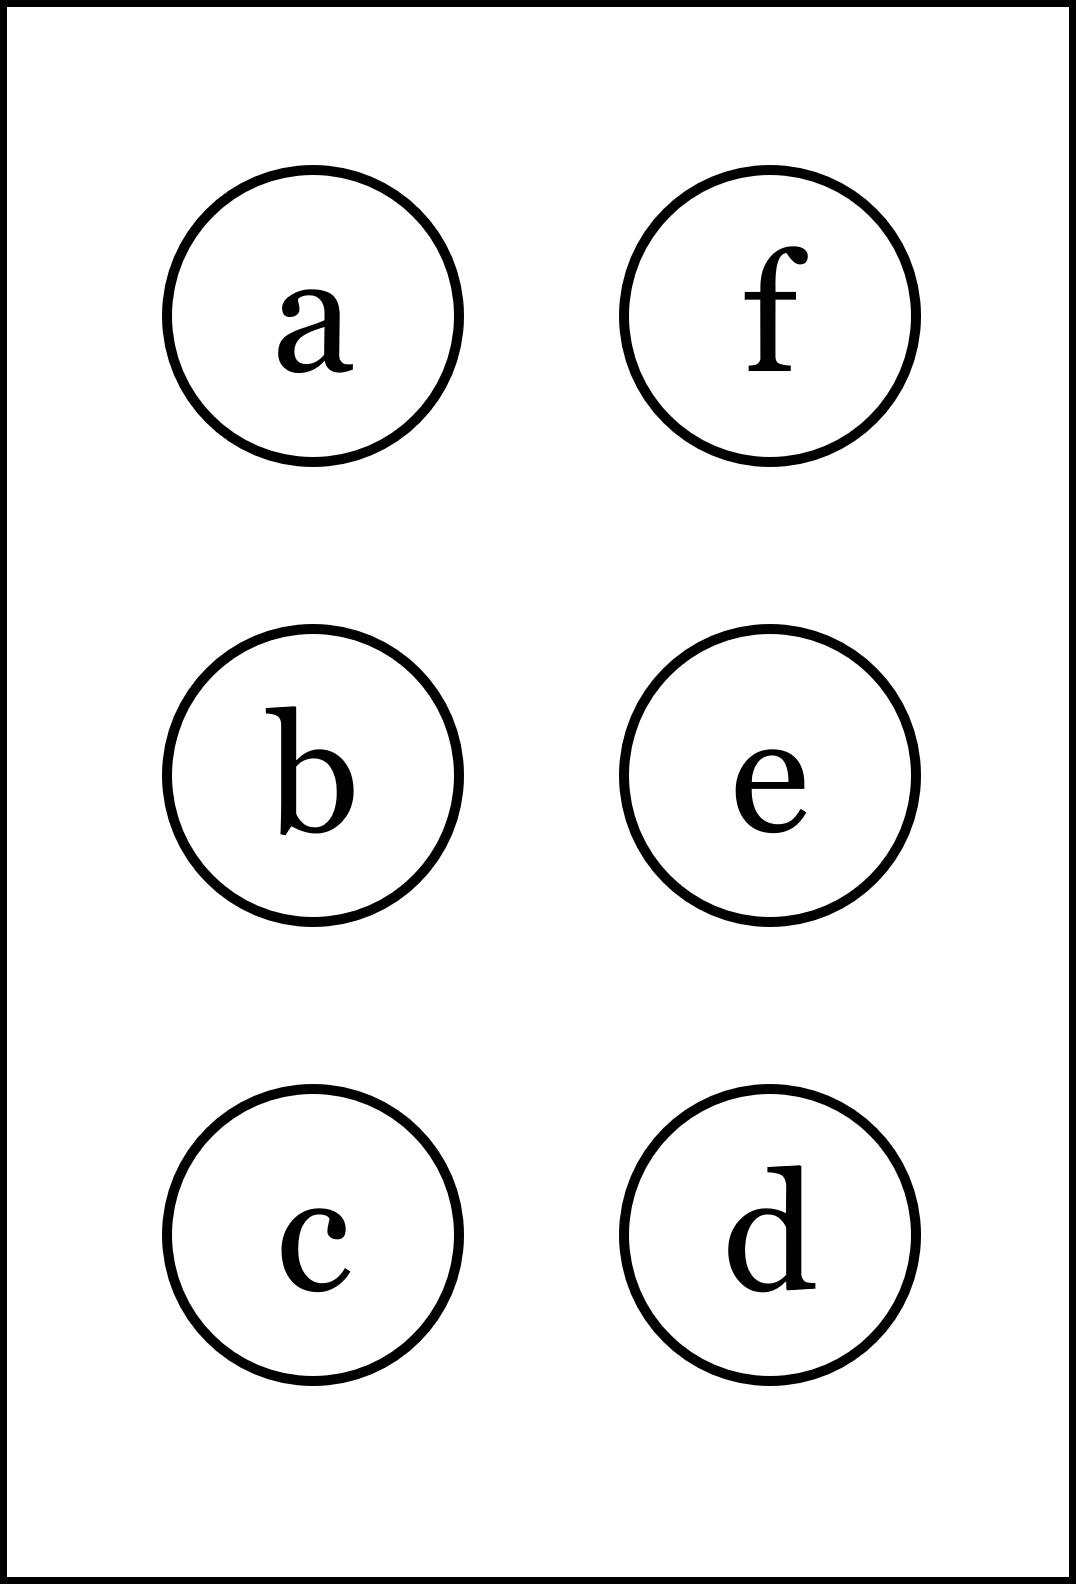
\includegraphics[height=40mm]{../images/braille.png}
{\small Písmeno Braillovej abecedy}
\end{center}
\end{minipage}
\end{center}
\end{minipage}
\\ \hdashline
\begin{minipage}[c][104.5mm][t]{0.5\linewidth}
\begin{center}
\vspace{7mm}
{\huge Kubická rovnice, skupina \textit{Kappa $\kappa$} -\romannumeral3}\\[5mm]
\textit{Jméno:}\phantom{xxxxxxxxxxxxxxxxxxxxxxxxxxxxxxxxxxxxxxxxxxxxxxxxxxxxxxxxxxxxxxxxx}\\[5mm]
\begin{minipage}{0.95\linewidth}
\begin{center}
\textbf{Vypočítej součet kořenů kubické rovnice.} Dvojitý kořen považuj do součtu za dva,\\trojitý kořen za tři. Pokud ti vyjde stejný výsledek jako je za otazníky, tak napravo\\barvi příslušející kroužek načerno. \textbf{Spolu odevzdejte výsledné slovo}.
\end{center}
\end{minipage}
\\[1mm]
\begin{minipage}{0.79\linewidth}
\begin{center}
\begin{varwidth}{\linewidth}
\begin{enumerate}
\Large
\item $-x^3-9x^2-18x=0$\quad \dotfill\; ???\;\dotfill \quad $3$
\item $2x^3-14x-12=0$\quad \dotfill\; ???\;\dotfill \quad $0$
\item $-6x^3+4x^2+54x-36=0$\quad \dotfill\; ???\;\dotfill \quad $\nicefrac{2}{3}$
\item $8x^3+20x^2-44x+16=0$\quad \dotfill\; ???\;\dotfill \quad $\nicefrac{-9}{2}$
\item \quad \dotfill\; ???\;\dotfill \quad vybarvi
\item \quad \dotfill\; ???\;\dotfill \quad vybarvi
\end{enumerate}
\end{varwidth}
\end{center}
\end{minipage}
\begin{minipage}{0.20\linewidth}
\begin{center}
{\Huge\bfseries 3.} \\[2mm]
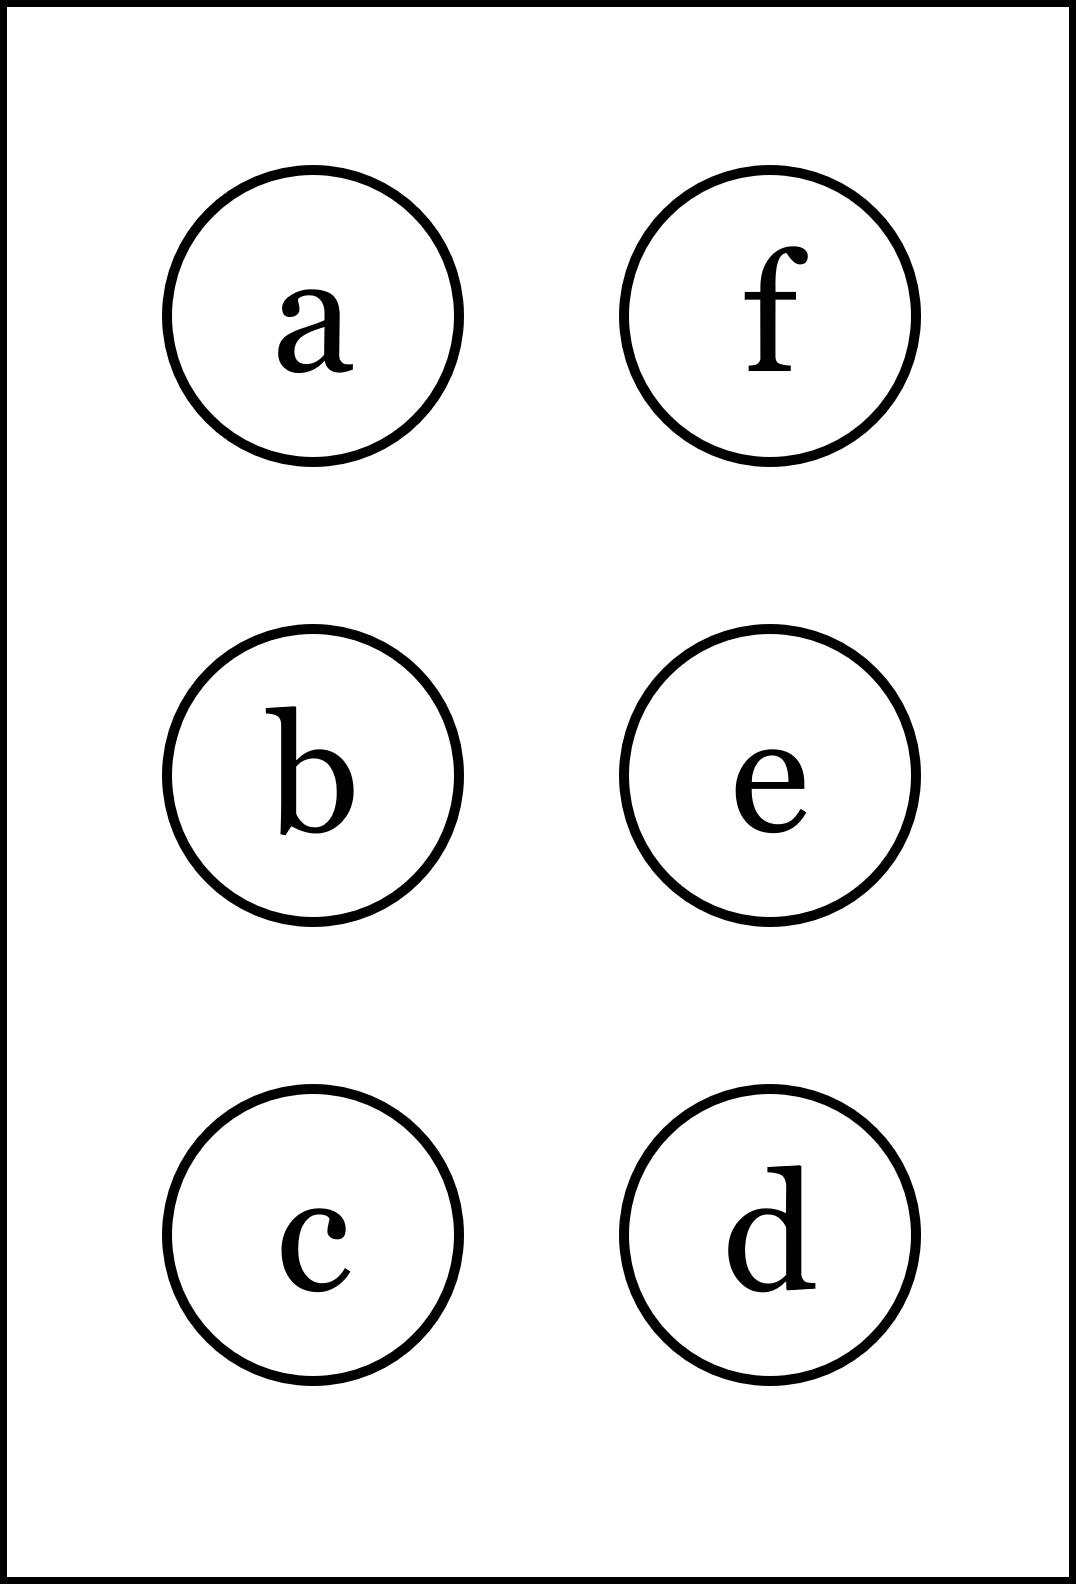
\includegraphics[height=40mm]{../images/braille.png}
{\small Písmeno Braillovej abecedy}
\end{center}
\end{minipage}
\end{center}
\end{minipage}
&
\begin{minipage}[c][104.5mm][t]{0.5\linewidth}
\begin{center}
\vspace{7mm}
{\huge Kubická rovnice, skupina \textit{Kappa $\kappa$} -\romannumeral4}\\[5mm]
\textit{Jméno:}\phantom{xxxxxxxxxxxxxxxxxxxxxxxxxxxxxxxxxxxxxxxxxxxxxxxxxxxxxxxxxxxxxxxxx}\\[5mm]
\begin{minipage}{0.95\linewidth}
\begin{center}
\textbf{Vypočítej součet kořenů kubické rovnice.} Dvojitý kořen považuj do součtu za dva,\\trojitý kořen za tři. Pokud ti vyjde stejný výsledek jako je za otazníky, tak napravo\\barvi příslušející kroužek načerno. \textbf{Spolu odevzdejte výsledné slovo}.
\end{center}
\end{minipage}
\\[1mm]
\begin{minipage}{0.79\linewidth}
\begin{center}
\begin{varwidth}{\linewidth}
\begin{enumerate}
\Large
\item $-2x^3-8x^2+24x=0$\quad \dotfill\; ???\;\dotfill \quad $8$
\item $-3x^3-24x^2-39x-18=0$\quad \dotfill\; ???\;\dotfill \quad $-6$
\item $7x^3-31x^2-62x-24=0$\quad \dotfill\; ???\;\dotfill \quad $\nicefrac{31}{7}$
\item $3x^3-10x^2-37x+60=0$\quad \dotfill\; ???\;\dotfill \quad $\nicefrac{-20}{3}$
\item \quad \dotfill\; ???\;\dotfill \quad nebarvi
\item \quad \dotfill\; ???\;\dotfill \quad vybarvi
\end{enumerate}
\end{varwidth}
\end{center}
\end{minipage}
\begin{minipage}{0.20\linewidth}
\begin{center}
{\Huge\bfseries 4.} \\[2mm]
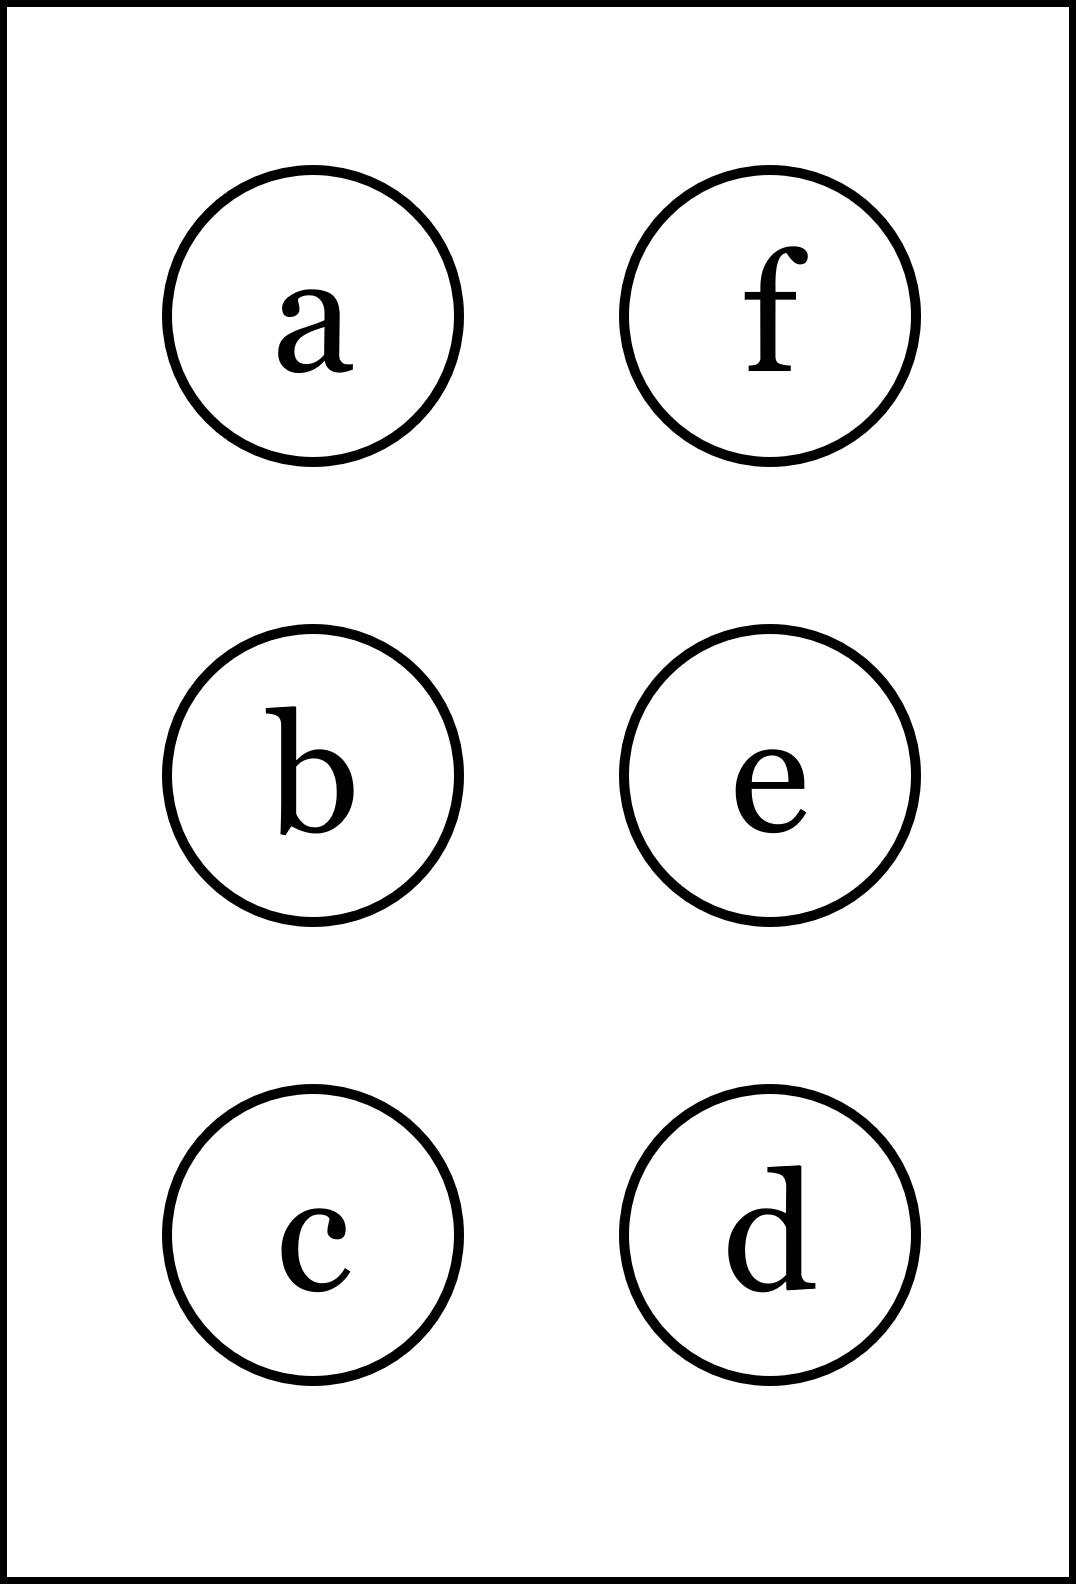
\includegraphics[height=40mm]{../images/braille.png}
{\small Písmeno Braillovej abecedy}
\end{center}
\end{minipage}
\end{center}
\end{minipage}
%
\end{tabular}
\newpage
\thispagestyle{empty}
\begin{tabular}{c:c}
\begin{minipage}[c][104.5mm][t]{0.5\linewidth}
\begin{center}
\vspace{7mm}
{\huge Kubická rovnice, skupina \textit{Lambda $\lambda$} -\romannumeral1}\\[5mm]
\textit{Jméno:}\phantom{xxxxxxxxxxxxxxxxxxxxxxxxxxxxxxxxxxxxxxxxxxxxxxxxxxxxxxxxxxxxxxxxx}\\[5mm]
\begin{minipage}{0.95\linewidth}
\begin{center}
\textbf{Vypočítej součet kořenů kubické rovnice.} Dvojitý kořen považuj do součtu za dva,\\trojitý kořen za tři. Pokud ti vyjde stejný výsledek jako je za otazníky, tak napravo\\barvi příslušející kroužek načerno. \textbf{Spolu odevzdejte výsledné slovo}.
\end{center}
\end{minipage}
\\[1mm]
\begin{minipage}{0.79\linewidth}
\begin{center}
\begin{varwidth}{\linewidth}
\begin{enumerate}
\Large
\item $4x^3+20x^2-24x=0$\quad \dotfill\; ???\;\dotfill \quad $-5$
\item $2x^3-6x^2-32x-24=0$\quad \dotfill\; ???\;\dotfill \quad $3$
\item $24x^3+56x^2-24x-56=0$\quad \dotfill\; ???\;\dotfill \quad $\nicefrac{-13}{3}$
\item $-21x^3+31x^2-11x+1=0$\quad \dotfill\; ???\;\dotfill \quad $\nicefrac{25}{21}$
\item \quad \dotfill\; ???\;\dotfill \quad nebarvi
\item \quad \dotfill\; ???\;\dotfill \quad nebarvi
\end{enumerate}
\end{varwidth}
\end{center}
\end{minipage}
\begin{minipage}{0.20\linewidth}
\begin{center}
{\Huge\bfseries 1.} \\[2mm]
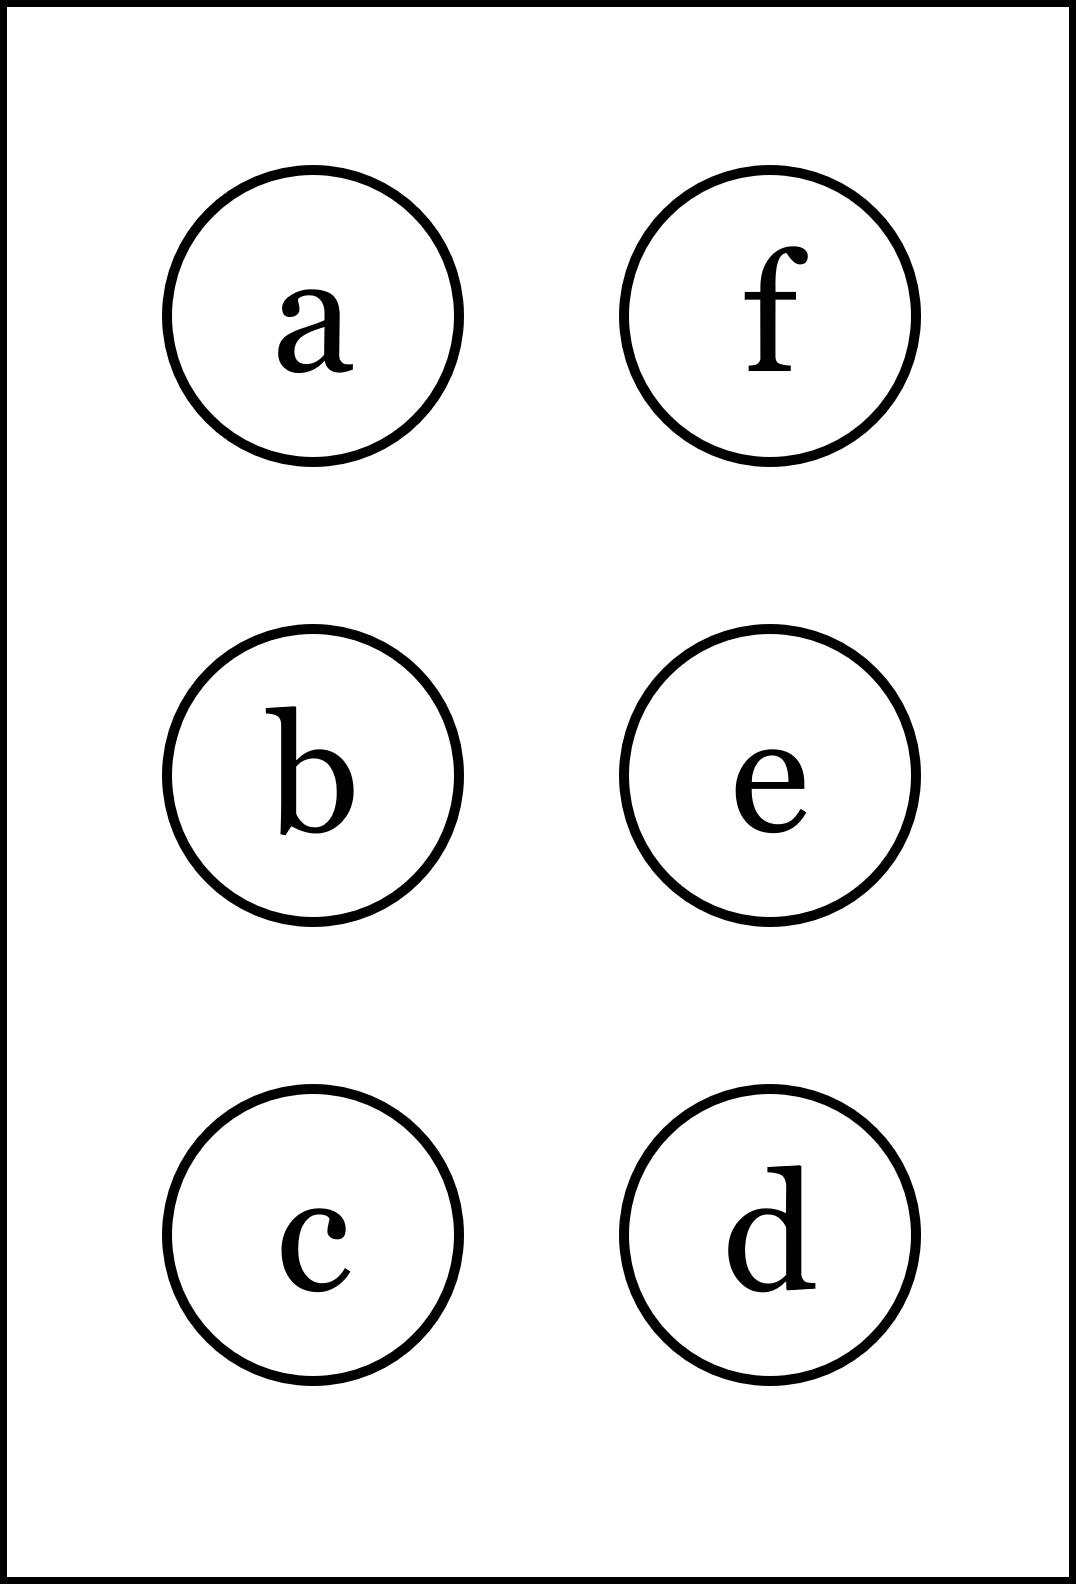
\includegraphics[height=40mm]{../images/braille.png}
{\small Písmeno Braillovej abecedy}
\end{center}
\end{minipage}
\end{center}
\end{minipage}
&
\begin{minipage}[c][104.5mm][t]{0.5\linewidth}
\begin{center}
\vspace{7mm}
{\huge Kubická rovnice, skupina \textit{Lambda $\lambda$} -\romannumeral2}\\[5mm]
\textit{Jméno:}\phantom{xxxxxxxxxxxxxxxxxxxxxxxxxxxxxxxxxxxxxxxxxxxxxxxxxxxxxxxxxxxxxxxxx}\\[5mm]
\begin{minipage}{0.95\linewidth}
\begin{center}
\textbf{Vypočítej součet kořenů kubické rovnice.} Dvojitý kořen považuj do součtu za dva,\\trojitý kořen za tři. Pokud ti vyjde stejný výsledek jako je za otazníky, tak napravo\\barvi příslušející kroužek načerno. \textbf{Spolu odevzdejte výsledné slovo}.
\end{center}
\end{minipage}
\\[1mm]
\begin{minipage}{0.79\linewidth}
\begin{center}
\begin{varwidth}{\linewidth}
\begin{enumerate}
\Large
\item $-2x^3+2x=0$\quad \dotfill\; ???\;\dotfill \quad $0$
\item $-x^3+2x^2+11x-12=0$\quad \dotfill\; ???\;\dotfill \quad $8$
\item $12x^3+72x^2+108x+48=0$\quad \dotfill\; ???\;\dotfill \quad $-4$
\item $-6x^3+35x^2-67x+42=0$\quad \dotfill\; ???\;\dotfill \quad $\nicefrac{35}{6}$
\item \quad \dotfill\; ???\;\dotfill \quad nebarvi
\item \quad \dotfill\; ???\;\dotfill \quad nebarvi
\end{enumerate}
\end{varwidth}
\end{center}
\end{minipage}
\begin{minipage}{0.20\linewidth}
\begin{center}
{\Huge\bfseries 2.} \\[2mm]
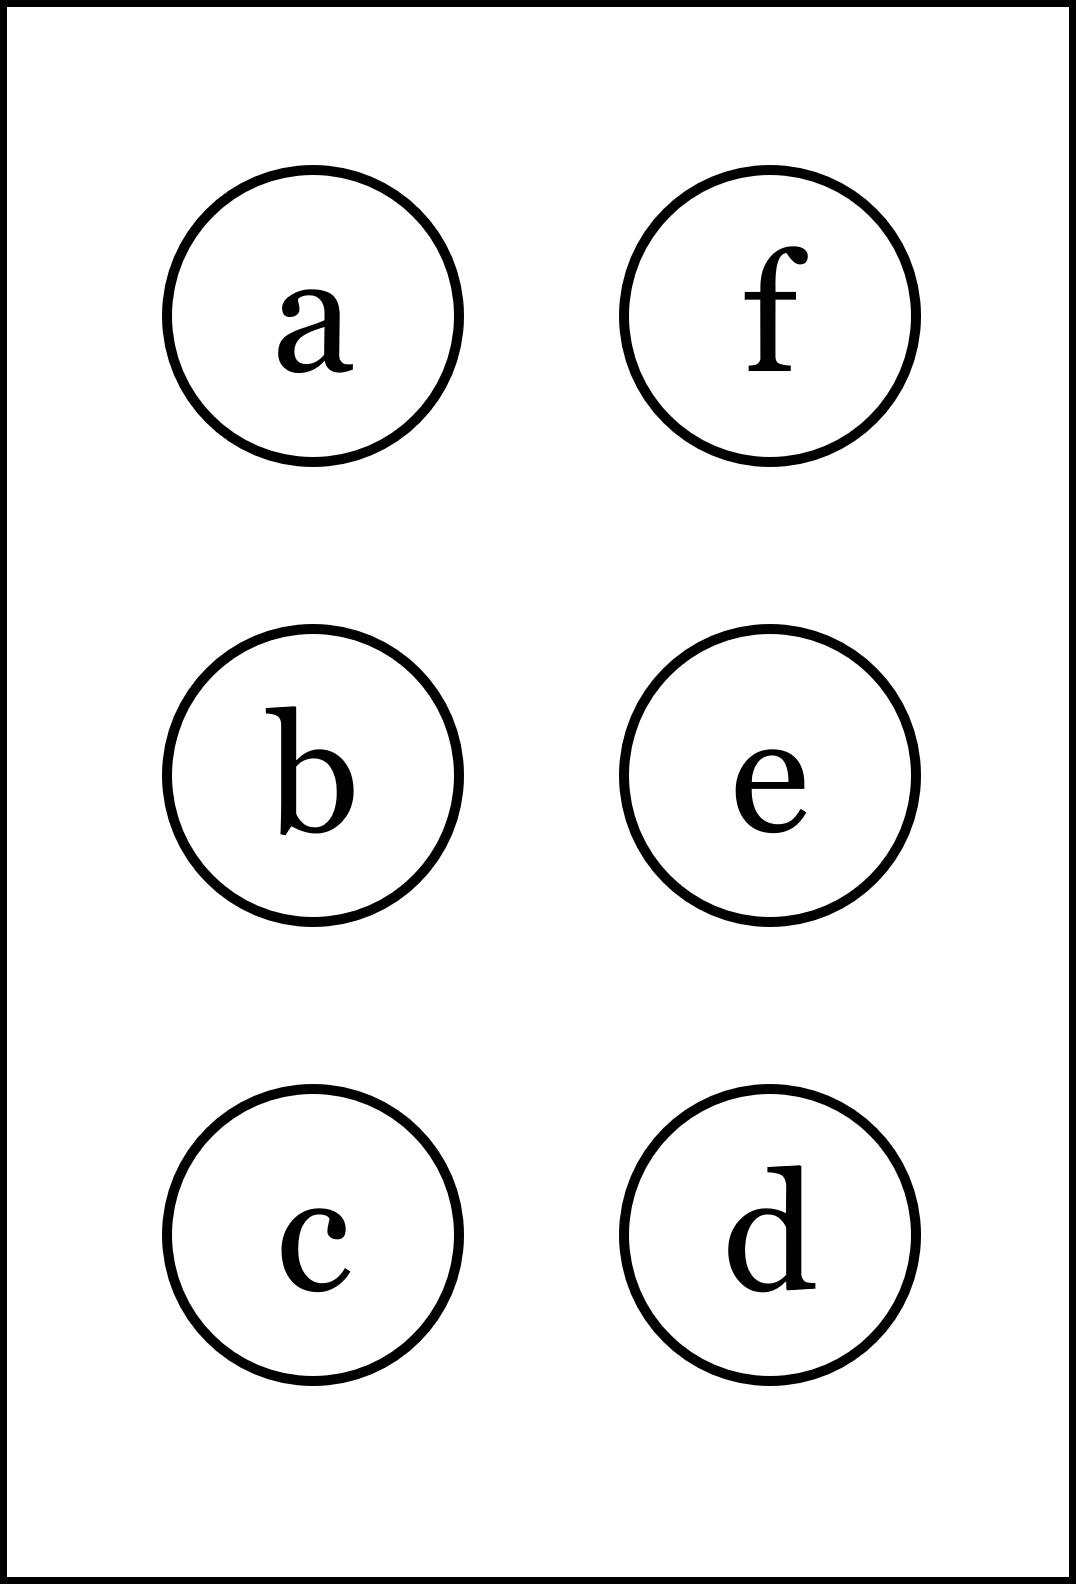
\includegraphics[height=40mm]{../images/braille.png}
{\small Písmeno Braillovej abecedy}
\end{center}
\end{minipage}
\end{center}
\end{minipage}
\\ \hdashline
\begin{minipage}[c][104.5mm][t]{0.5\linewidth}
\begin{center}
\vspace{7mm}
{\huge Kubická rovnice, skupina \textit{Lambda $\lambda$} -\romannumeral3}\\[5mm]
\textit{Jméno:}\phantom{xxxxxxxxxxxxxxxxxxxxxxxxxxxxxxxxxxxxxxxxxxxxxxxxxxxxxxxxxxxxxxxxx}\\[5mm]
\begin{minipage}{0.95\linewidth}
\begin{center}
\textbf{Vypočítej součet kořenů kubické rovnice.} Dvojitý kořen považuj do součtu za dva,\\trojitý kořen za tři. Pokud ti vyjde stejný výsledek jako je za otazníky, tak napravo\\barvi příslušející kroužek načerno. \textbf{Spolu odevzdejte výsledné slovo}.
\end{center}
\end{minipage}
\\[1mm]
\begin{minipage}{0.79\linewidth}
\begin{center}
\begin{varwidth}{\linewidth}
\begin{enumerate}
\Large
\item $-x^3-6x^2-5x=0$\quad \dotfill\; ???\;\dotfill \quad $-6$
\item $-2x^3+8x^2+22x-60=0$\quad \dotfill\; ???\;\dotfill \quad $4$
\item $6x^3+44x^2+78x+40=0$\quad \dotfill\; ???\;\dotfill \quad $\nicefrac{-14}{3}$
\item $-15x^3-49x^2-9x+9=0$\quad \dotfill\; ???\;\dotfill \quad $\nicefrac{-59}{15}$
\item \quad \dotfill\; ???\;\dotfill \quad nebarvi
\item \quad \dotfill\; ???\;\dotfill \quad nebarvi
\end{enumerate}
\end{varwidth}
\end{center}
\end{minipage}
\begin{minipage}{0.20\linewidth}
\begin{center}
{\Huge\bfseries 3.} \\[2mm]
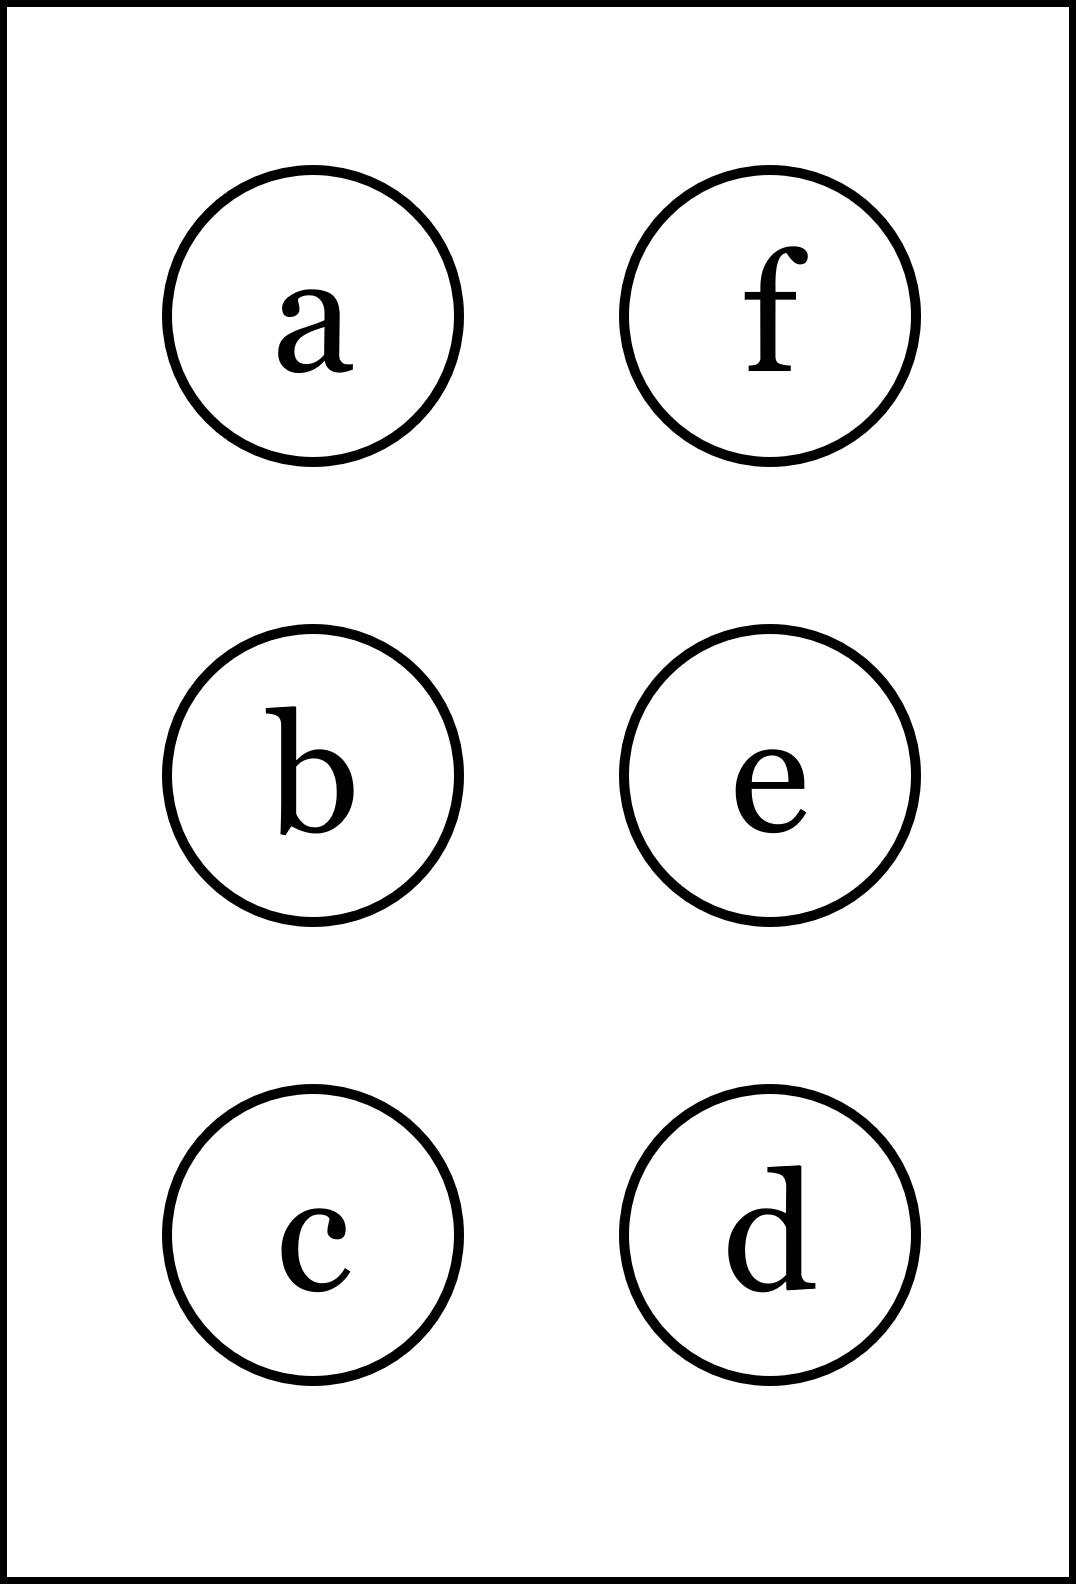
\includegraphics[height=40mm]{../images/braille.png}
{\small Písmeno Braillovej abecedy}
\end{center}
\end{minipage}
\end{center}
\end{minipage}
&
\begin{minipage}[c][104.5mm][t]{0.5\linewidth}
\begin{center}
\vspace{7mm}
{\huge Kubická rovnice, skupina \textit{Lambda $\lambda$} -\romannumeral4}\\[5mm]
\textit{Jméno:}\phantom{xxxxxxxxxxxxxxxxxxxxxxxxxxxxxxxxxxxxxxxxxxxxxxxxxxxxxxxxxxxxxxxxx}\\[5mm]
\begin{minipage}{0.95\linewidth}
\begin{center}
\textbf{Vypočítej součet kořenů kubické rovnice.} Dvojitý kořen považuj do součtu za dva,\\trojitý kořen za tři. Pokud ti vyjde stejný výsledek jako je za otazníky, tak napravo\\barvi příslušející kroužek načerno. \textbf{Spolu odevzdejte výsledné slovo}.
\end{center}
\end{minipage}
\\[1mm]
\begin{minipage}{0.79\linewidth}
\begin{center}
\begin{varwidth}{\linewidth}
\begin{enumerate}
\Large
\item $7x^3-14x^2+7x=0$\quad \dotfill\; ???\;\dotfill \quad $2$
\item $5x^3+25x^2-5x-25=0$\quad \dotfill\; ???\;\dotfill \quad $-7$
\item $8x^3+14x^2-28x+6=0$\quad \dotfill\; ???\;\dotfill \quad $\nicefrac{-15}{4}$
\item $-8x^3-66x^2-73x-21=0$\quad \dotfill\; ???\;\dotfill \quad $\nicefrac{-29}{4}$
\item \quad \dotfill\; ???\;\dotfill \quad nebarvi
\item \quad \dotfill\; ???\;\dotfill \quad nebarvi
\end{enumerate}
\end{varwidth}
\end{center}
\end{minipage}
\begin{minipage}{0.20\linewidth}
\begin{center}
{\Huge\bfseries 4.} \\[2mm]
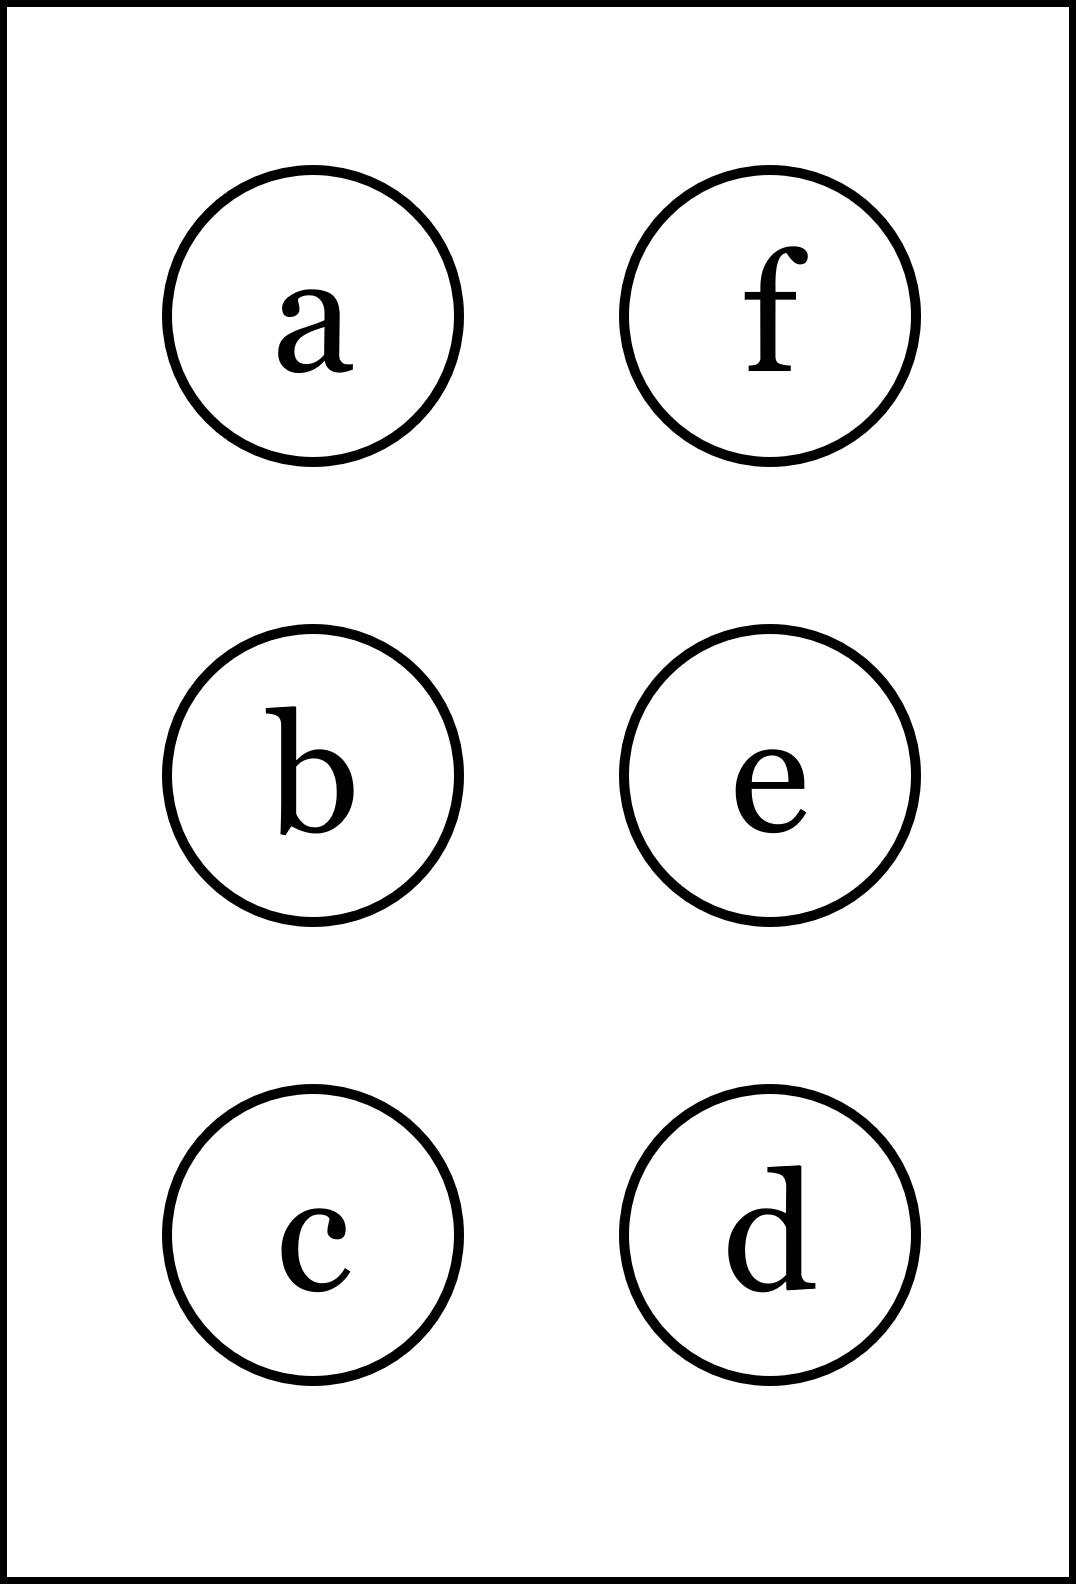
\includegraphics[height=40mm]{../images/braille.png}
{\small Písmeno Braillovej abecedy}
\end{center}
\end{minipage}
\end{center}
\end{minipage}
%
\end{tabular}
\newpage
\thispagestyle{empty}
\begin{tabular}{c:c}
\begin{minipage}[c][104.5mm][t]{0.5\linewidth}
\begin{center}
\vspace{7mm}
{\huge Kubická rovnice, skupina \textit{Mu $\mu$} -\romannumeral1}\\[5mm]
\textit{Jméno:}\phantom{xxxxxxxxxxxxxxxxxxxxxxxxxxxxxxxxxxxxxxxxxxxxxxxxxxxxxxxxxxxxxxxxx}\\[5mm]
\begin{minipage}{0.95\linewidth}
\begin{center}
\textbf{Vypočítej součet kořenů kubické rovnice.} Dvojitý kořen považuj do součtu za dva,\\trojitý kořen za tři. Pokud ti vyjde stejný výsledek jako je za otazníky, tak napravo\\barvi příslušející kroužek načerno. \textbf{Spolu odevzdejte výsledné slovo}.
\end{center}
\end{minipage}
\\[1mm]
\begin{minipage}{0.79\linewidth}
\begin{center}
\begin{varwidth}{\linewidth}
\begin{enumerate}
\Large
\item $-3x^3-15x^2+18x=0$\quad \dotfill\; ???\;\dotfill \quad $-5$
\item $2x^3-4x^2-2x+4=0$\quad \dotfill\; ???\;\dotfill \quad $2$
\item $4x^3+4x^2-29x+21=0$\quad \dotfill\; ???\;\dotfill \quad $6$
\item $5x^3+10x^2-5x-10=0$\quad \dotfill\; ???\;\dotfill \quad $-4$
\item \quad \dotfill\; ???\;\dotfill \quad nebarvi
\item \quad \dotfill\; ???\;\dotfill \quad vybarvi
\end{enumerate}
\end{varwidth}
\end{center}
\end{minipage}
\begin{minipage}{0.20\linewidth}
\begin{center}
{\Huge\bfseries 1.} \\[2mm]
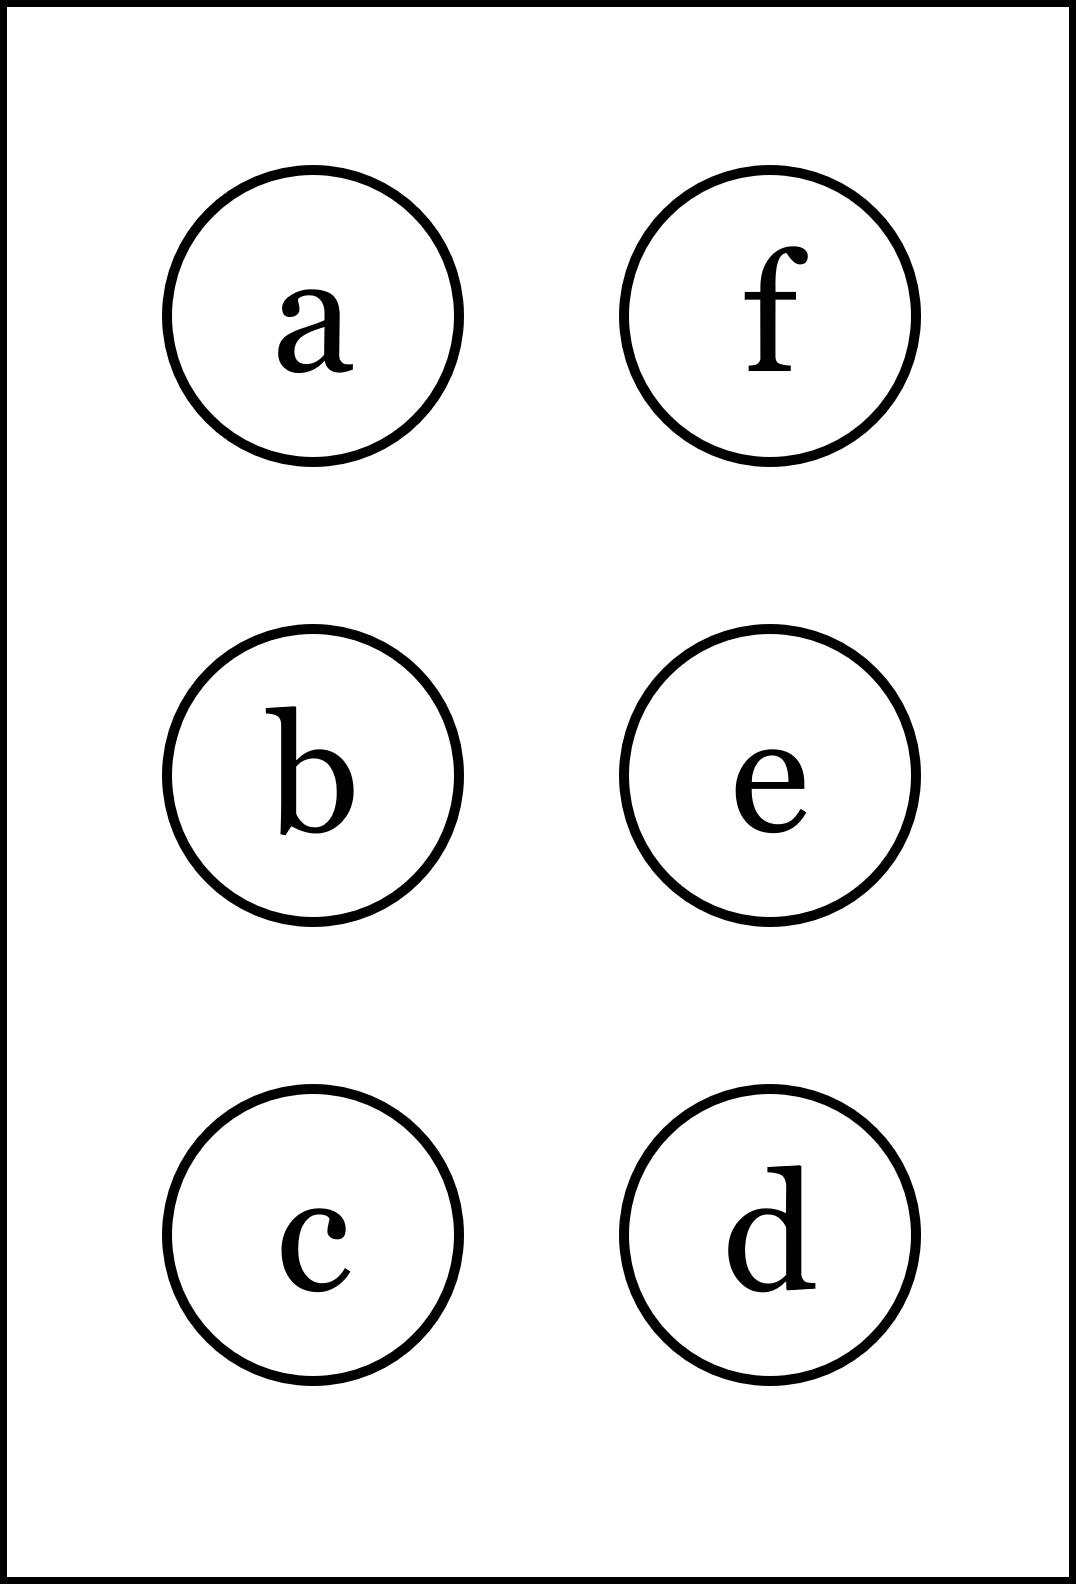
\includegraphics[height=40mm]{../images/braille.png}
{\small Písmeno Braillovej abecedy}
\end{center}
\end{minipage}
\end{center}
\end{minipage}
&
\begin{minipage}[c][104.5mm][t]{0.5\linewidth}
\begin{center}
\vspace{7mm}
{\huge Kubická rovnice, skupina \textit{Mu $\mu$} -\romannumeral2}\\[5mm]
\textit{Jméno:}\phantom{xxxxxxxxxxxxxxxxxxxxxxxxxxxxxxxxxxxxxxxxxxxxxxxxxxxxxxxxxxxxxxxxx}\\[5mm]
\begin{minipage}{0.95\linewidth}
\begin{center}
\textbf{Vypočítej součet kořenů kubické rovnice.} Dvojitý kořen považuj do součtu za dva,\\trojitý kořen za tři. Pokud ti vyjde stejný výsledek jako je za otazníky, tak napravo\\barvi příslušející kroužek načerno. \textbf{Spolu odevzdejte výsledné slovo}.
\end{center}
\end{minipage}
\\[1mm]
\begin{minipage}{0.79\linewidth}
\begin{center}
\begin{varwidth}{\linewidth}
\begin{enumerate}
\Large
\item $-3x^3+15x^2-18x=0$\quad \dotfill\; ???\;\dotfill \quad $1$
\item $x^3-14x^2+53x-40=0$\quad \dotfill\; ???\;\dotfill \quad $14$
\item $-8x^3-20x^2+8x+20=0$\quad \dotfill\; ???\;\dotfill \quad $\nicefrac{5}{2}$
\item $7x^3-22x^2-25x+4=0$\quad \dotfill\; ???\;\dotfill \quad $\nicefrac{20}{7}$
\item \quad \dotfill\; ???\;\dotfill \quad nebarvi
\item \quad \dotfill\; ???\;\dotfill \quad vybarvi
\end{enumerate}
\end{varwidth}
\end{center}
\end{minipage}
\begin{minipage}{0.20\linewidth}
\begin{center}
{\Huge\bfseries 2.} \\[2mm]
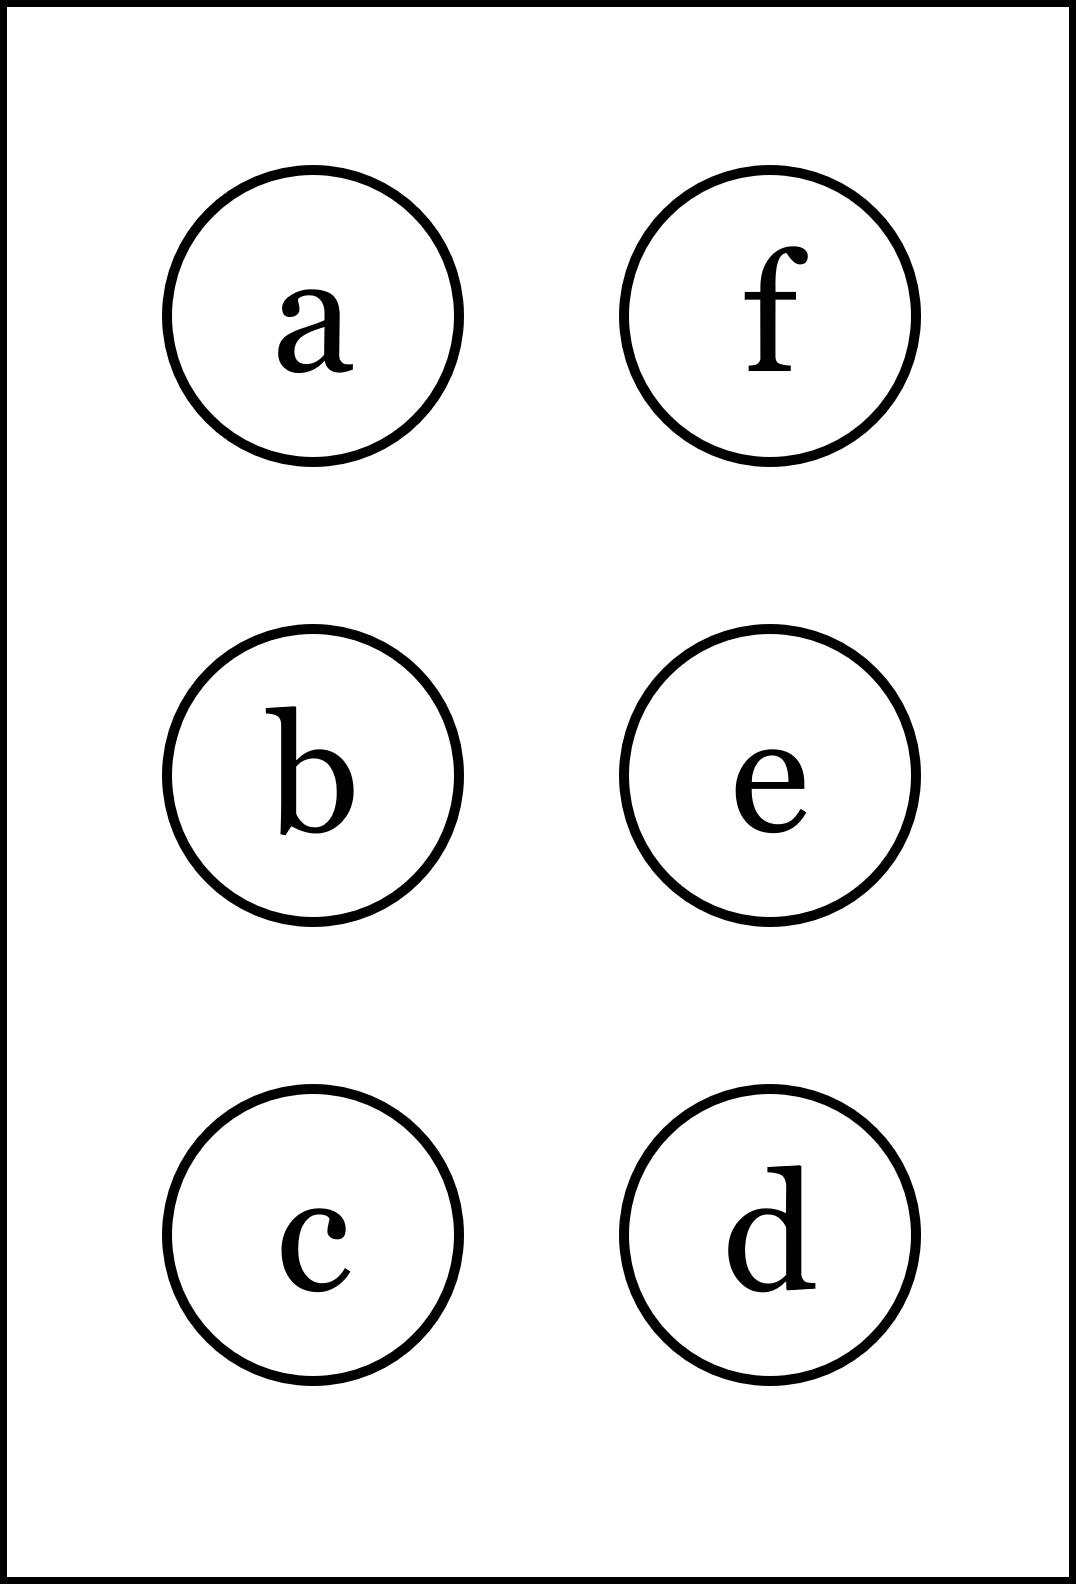
\includegraphics[height=40mm]{../images/braille.png}
{\small Písmeno Braillovej abecedy}
\end{center}
\end{minipage}
\end{center}
\end{minipage}
\\ \hdashline
\begin{minipage}[c][104.5mm][t]{0.5\linewidth}
\begin{center}
\vspace{7mm}
{\huge Kubická rovnice, skupina \textit{Mu $\mu$} -\romannumeral3}\\[5mm]
\textit{Jméno:}\phantom{xxxxxxxxxxxxxxxxxxxxxxxxxxxxxxxxxxxxxxxxxxxxxxxxxxxxxxxxxxxxxxxxx}\\[5mm]
\begin{minipage}{0.95\linewidth}
\begin{center}
\textbf{Vypočítej součet kořenů kubické rovnice.} Dvojitý kořen považuj do součtu za dva,\\trojitý kořen za tři. Pokud ti vyjde stejný výsledek jako je za otazníky, tak napravo\\barvi příslušející kroužek načerno. \textbf{Spolu odevzdejte výsledné slovo}.
\end{center}
\end{minipage}
\\[1mm]
\begin{minipage}{0.79\linewidth}
\begin{center}
\begin{varwidth}{\linewidth}
\begin{enumerate}
\Large
\item $x^3-9x=0$\quad \dotfill\; ???\;\dotfill \quad $0$
\item $-2x^3+4x^2+8x-16=0$\quad \dotfill\; ???\;\dotfill \quad $2$
\item $12x^3+20x^2-44x+12=0$\quad \dotfill\; ???\;\dotfill \quad $\nicefrac{-5}{3}$
\item $3x^3+12x^2-57x+42=0$\quad \dotfill\; ???\;\dotfill \quad $10$
\item \quad \dotfill\; ???\;\dotfill \quad nebarvi
\item \quad \dotfill\; ???\;\dotfill \quad nebarvi
\end{enumerate}
\end{varwidth}
\end{center}
\end{minipage}
\begin{minipage}{0.20\linewidth}
\begin{center}
{\Huge\bfseries 3.} \\[2mm]
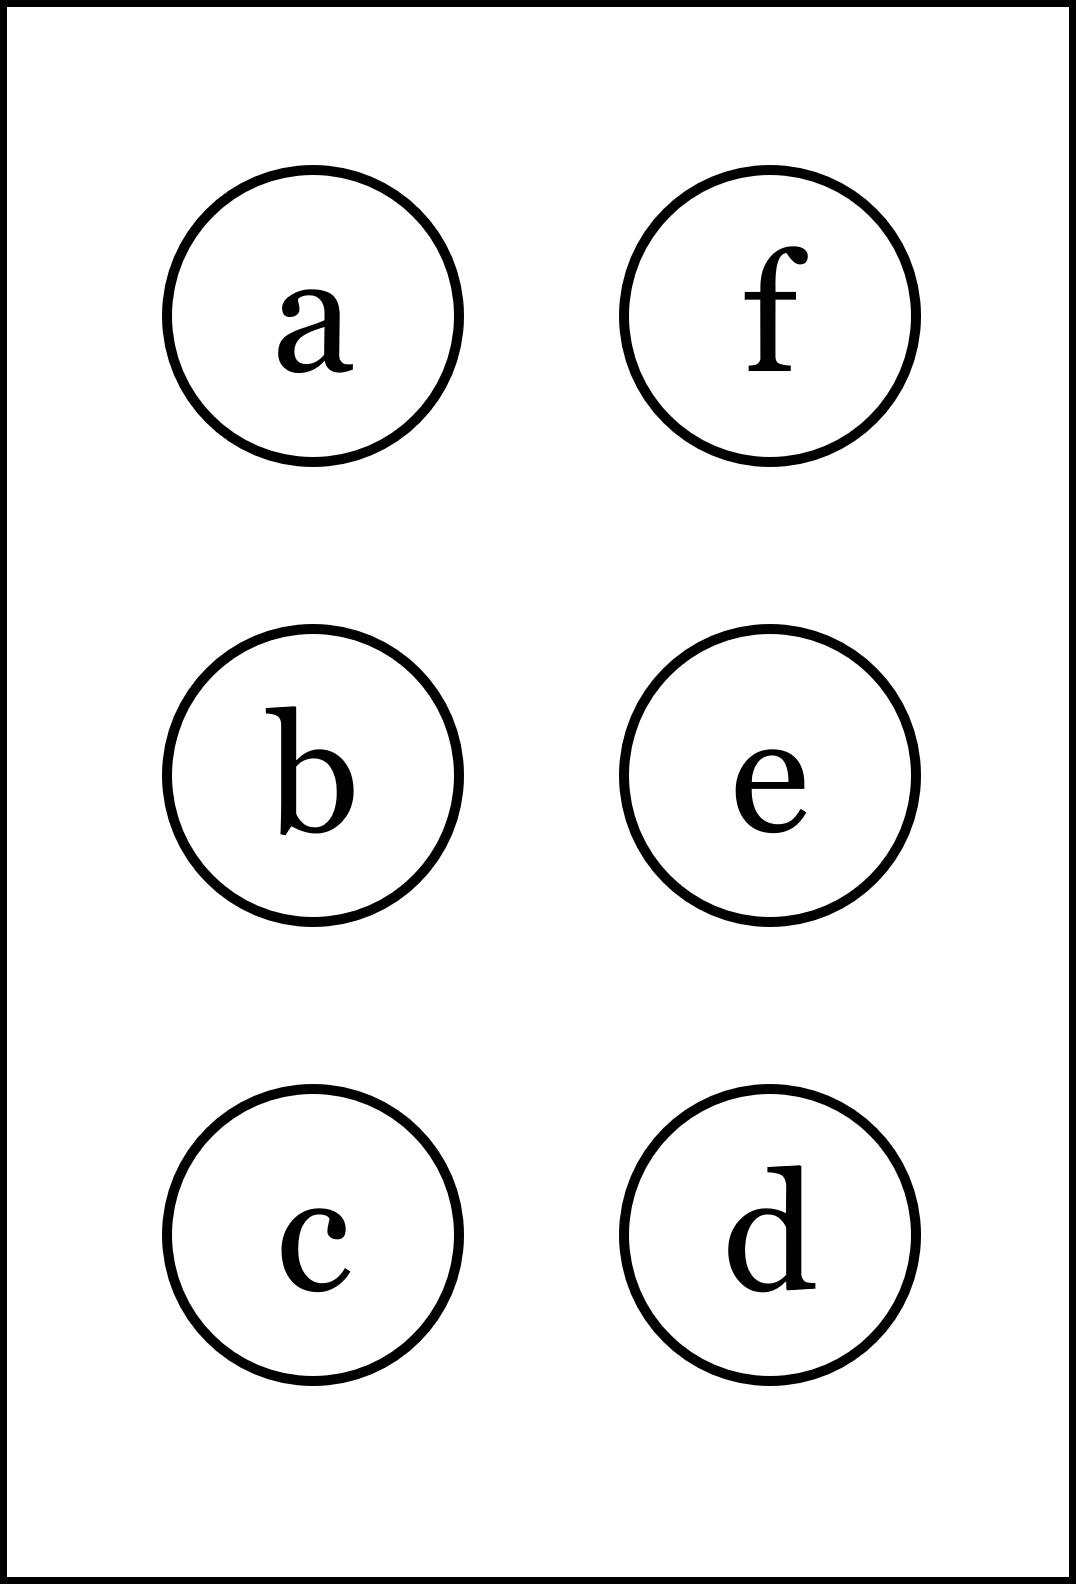
\includegraphics[height=40mm]{../images/braille.png}
{\small Písmeno Braillovej abecedy}
\end{center}
\end{minipage}
\end{center}
\end{minipage}
&
\begin{minipage}[c][104.5mm][t]{0.5\linewidth}
\begin{center}
\vspace{7mm}
{\huge Kubická rovnice, skupina \textit{Mu $\mu$} -\romannumeral4}\\[5mm]
\textit{Jméno:}\phantom{xxxxxxxxxxxxxxxxxxxxxxxxxxxxxxxxxxxxxxxxxxxxxxxxxxxxxxxxxxxxxxxxx}\\[5mm]
\begin{minipage}{0.95\linewidth}
\begin{center}
\textbf{Vypočítej součet kořenů kubické rovnice.} Dvojitý kořen považuj do součtu za dva,\\trojitý kořen za tři. Pokud ti vyjde stejný výsledek jako je za otazníky, tak napravo\\barvi příslušející kroužek načerno. \textbf{Spolu odevzdejte výsledné slovo}.
\end{center}
\end{minipage}
\\[1mm]
\begin{minipage}{0.79\linewidth}
\begin{center}
\begin{varwidth}{\linewidth}
\begin{enumerate}
\Large
\item $-3x^3+3x^2+36x=0$\quad \dotfill\; ???\;\dotfill \quad $1$
\item $x^3-11x^2+26x-16=0$\quad \dotfill\; ???\;\dotfill \quad $7$
\item $7x^3+20x^2-31x+4=0$\quad \dotfill\; ???\;\dotfill \quad $\nicefrac{-20}{7}$
\item $-5x^3+x^2+14x+8=0$\quad \dotfill\; ???\;\dotfill \quad $\nicefrac{9}{5}$
\item \quad \dotfill\; ???\;\dotfill \quad nebarvi
\item \quad \dotfill\; ???\;\dotfill \quad vybarvi
\end{enumerate}
\end{varwidth}
\end{center}
\end{minipage}
\begin{minipage}{0.20\linewidth}
\begin{center}
{\Huge\bfseries 4.} \\[2mm]
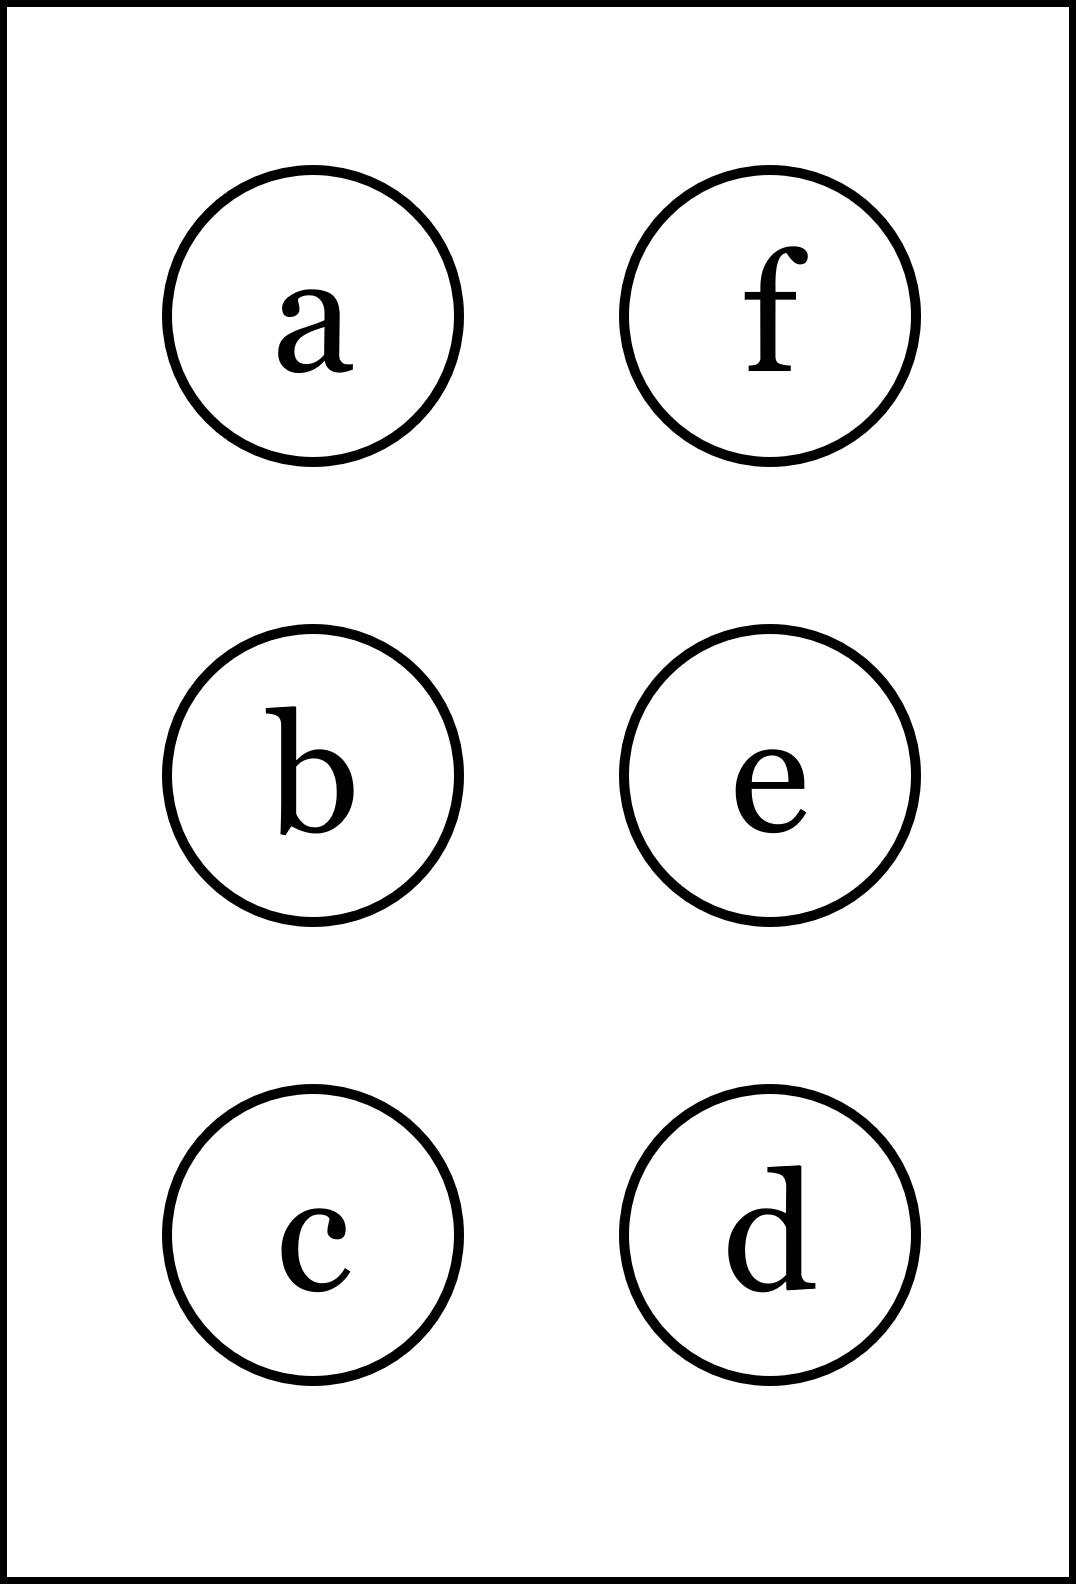
\includegraphics[height=40mm]{../images/braille.png}
{\small Písmeno Braillovej abecedy}
\end{center}
\end{minipage}
\end{center}
\end{minipage}
%
\end{tabular}
\newpage
\thispagestyle{empty}
\begin{tabular}{c:c}
\begin{minipage}[c][104.5mm][t]{0.5\linewidth}
\begin{center}
\vspace{7mm}
{\huge Kubická rovnice, skupina \textit{Nu $\nu$} -\romannumeral1}\\[5mm]
\textit{Jméno:}\phantom{xxxxxxxxxxxxxxxxxxxxxxxxxxxxxxxxxxxxxxxxxxxxxxxxxxxxxxxxxxxxxxxxx}\\[5mm]
\begin{minipage}{0.95\linewidth}
\begin{center}
\textbf{Vypočítej součet kořenů kubické rovnice.} Dvojitý kořen považuj do součtu za dva,\\trojitý kořen za tři. Pokud ti vyjde stejný výsledek jako je za otazníky, tak napravo\\barvi příslušející kroužek načerno. \textbf{Spolu odevzdejte výsledné slovo}.
\end{center}
\end{minipage}
\\[1mm]
\begin{minipage}{0.79\linewidth}
\begin{center}
\begin{varwidth}{\linewidth}
\begin{enumerate}
\Large
\item $5x^3-25x^2+30x=0$\quad \dotfill\; ???\;\dotfill \quad $1$
\item $2x^3-4x^2-10x+12=0$\quad \dotfill\; ???\;\dotfill \quad $-4$
\item $30x^3+48x^2+6x-12=0$\quad \dotfill\; ???\;\dotfill \quad $\nicefrac{-8}{5}$
\item $-5x^3-4x^2+52x-48=0$\quad \dotfill\; ???\;\dotfill \quad $\nicefrac{-4}{5}$
\item \quad \dotfill\; ???\;\dotfill \quad nebarvi
\item \quad \dotfill\; ???\;\dotfill \quad vybarvi
\end{enumerate}
\end{varwidth}
\end{center}
\end{minipage}
\begin{minipage}{0.20\linewidth}
\begin{center}
{\Huge\bfseries 1.} \\[2mm]
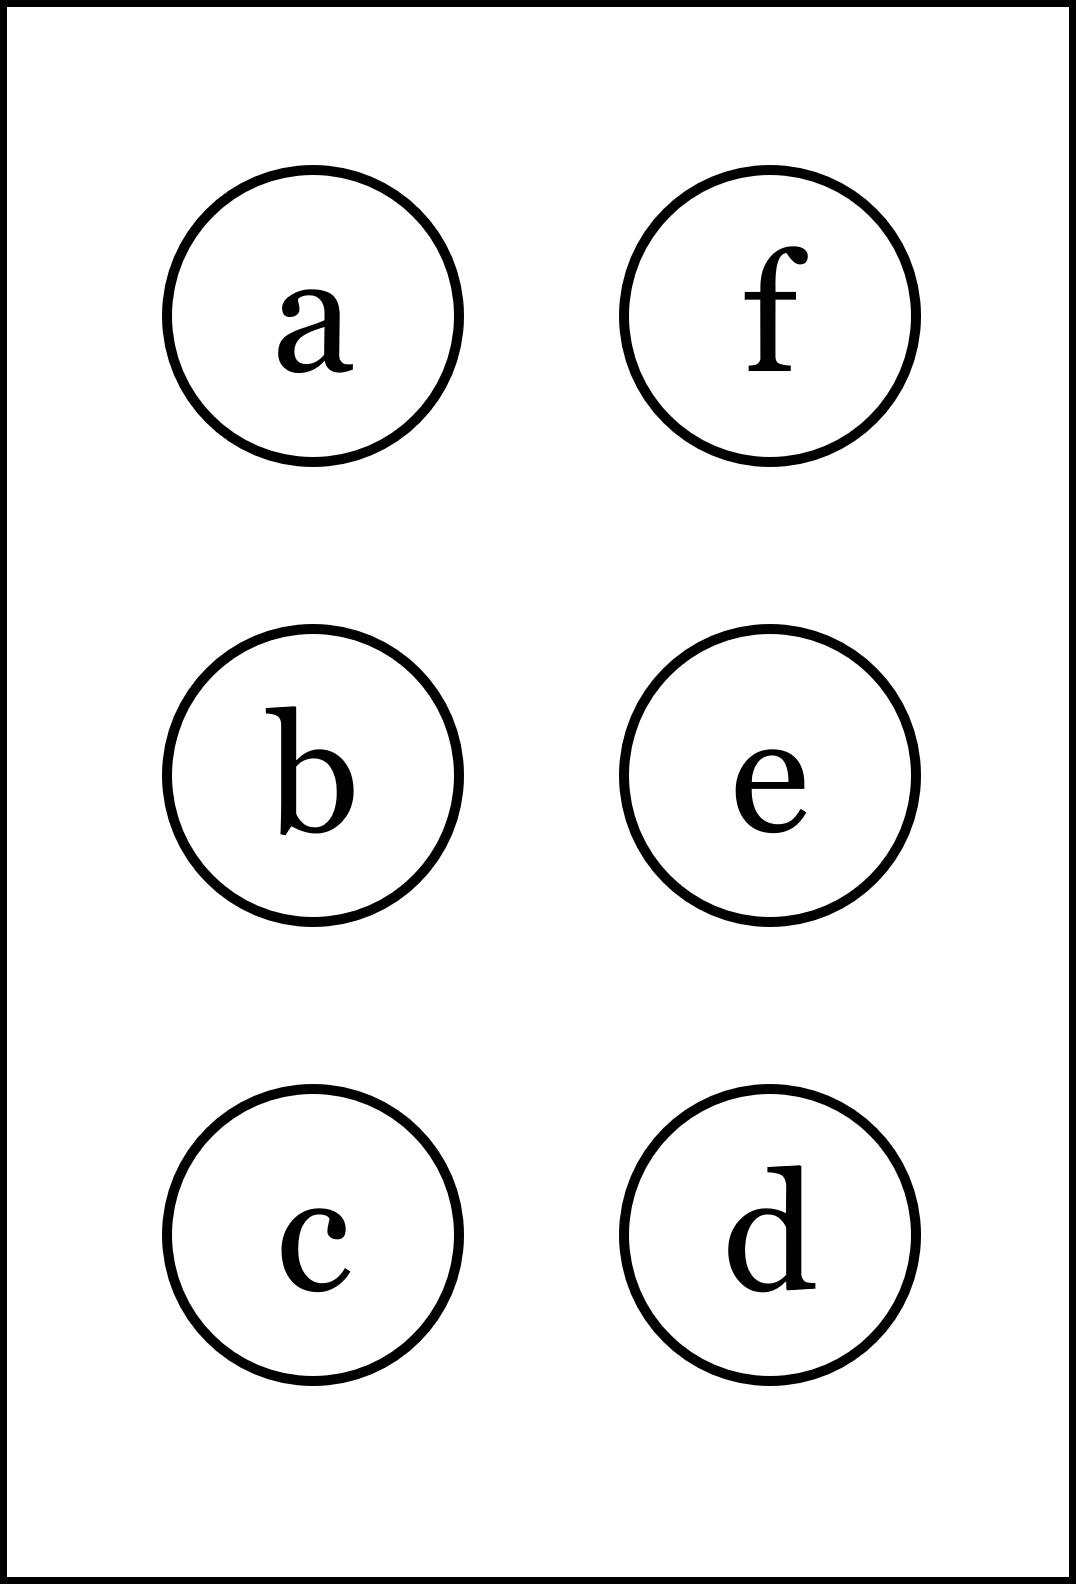
\includegraphics[height=40mm]{../images/braille.png}
{\small Písmeno Braillovej abecedy}
\end{center}
\end{minipage}
\end{center}
\end{minipage}
&
\begin{minipage}[c][104.5mm][t]{0.5\linewidth}
\begin{center}
\vspace{7mm}
{\huge Kubická rovnice, skupina \textit{Nu $\nu$} -\romannumeral2}\\[5mm]
\textit{Jméno:}\phantom{xxxxxxxxxxxxxxxxxxxxxxxxxxxxxxxxxxxxxxxxxxxxxxxxxxxxxxxxxxxxxxxxx}\\[5mm]
\begin{minipage}{0.95\linewidth}
\begin{center}
\textbf{Vypočítej součet kořenů kubické rovnice.} Dvojitý kořen považuj do součtu za dva,\\trojitý kořen za tři. Pokud ti vyjde stejný výsledek jako je za otazníky, tak napravo\\barvi příslušející kroužek načerno. \textbf{Spolu odevzdejte výsledné slovo}.
\end{center}
\end{minipage}
\\[1mm]
\begin{minipage}{0.79\linewidth}
\begin{center}
\begin{varwidth}{\linewidth}
\begin{enumerate}
\Large
\item $x^3+5x^2+4x=0$\quad \dotfill\; ???\;\dotfill \quad $-3$
\item $-7x^3+7x^2+28x-28=0$\quad \dotfill\; ???\;\dotfill \quad $1$
\item $-40x^3-31x^2+18x+9=0$\quad \dotfill\; ???\;\dotfill \quad $\nicefrac{-31}{40}$
\item $-24x^3+17x^2+76x+35=0$\quad \dotfill\; ???\;\dotfill \quad $\nicefrac{47}{24}$
\item \quad \dotfill\; ???\;\dotfill \quad nebarvi
\item \quad \dotfill\; ???\;\dotfill \quad vybarvi
\end{enumerate}
\end{varwidth}
\end{center}
\end{minipage}
\begin{minipage}{0.20\linewidth}
\begin{center}
{\Huge\bfseries 2.} \\[2mm]
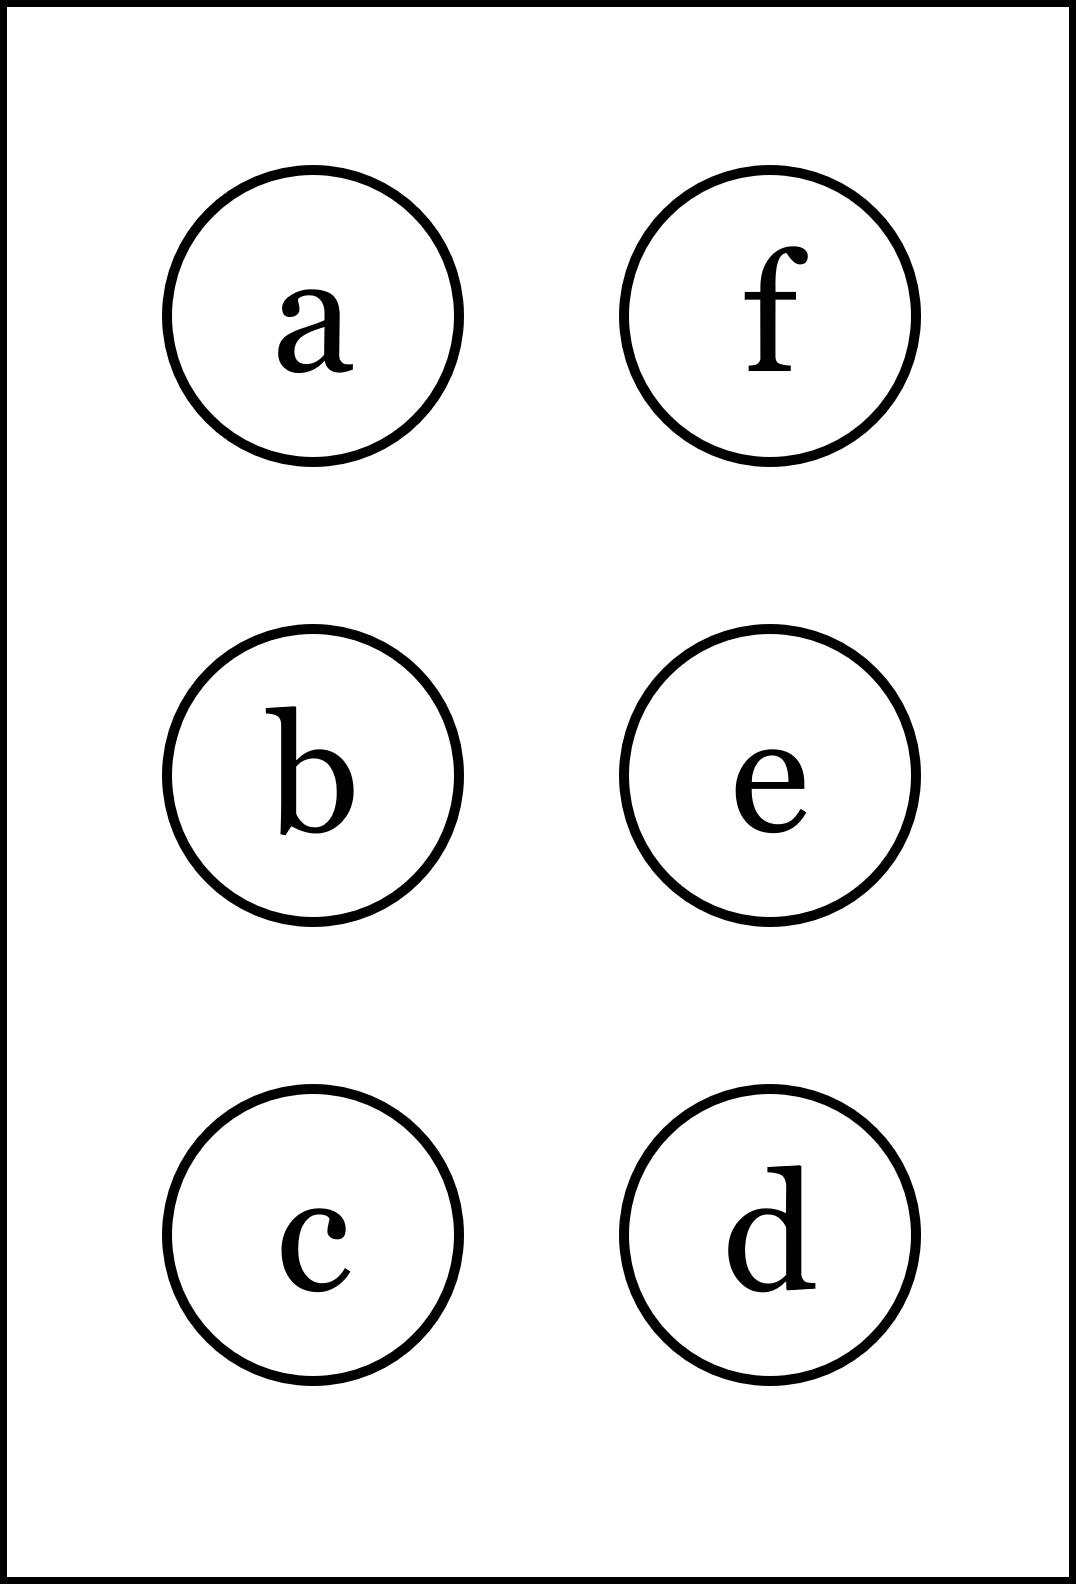
\includegraphics[height=40mm]{../images/braille.png}
{\small Písmeno Braillovej abecedy}
\end{center}
\end{minipage}
\end{center}
\end{minipage}
\\ \hdashline
\begin{minipage}[c][104.5mm][t]{0.5\linewidth}
\begin{center}
\vspace{7mm}
{\huge Kubická rovnice, skupina \textit{Nu $\nu$} -\romannumeral3}\\[5mm]
\textit{Jméno:}\phantom{xxxxxxxxxxxxxxxxxxxxxxxxxxxxxxxxxxxxxxxxxxxxxxxxxxxxxxxxxxxxxxxxx}\\[5mm]
\begin{minipage}{0.95\linewidth}
\begin{center}
\textbf{Vypočítej součet kořenů kubické rovnice.} Dvojitý kořen považuj do součtu za dva,\\trojitý kořen za tři. Pokud ti vyjde stejný výsledek jako je za otazníky, tak napravo\\barvi příslušející kroužek načerno. \textbf{Spolu odevzdejte výsledné slovo}.
\end{center}
\end{minipage}
\\[1mm]
\begin{minipage}{0.79\linewidth}
\begin{center}
\begin{varwidth}{\linewidth}
\begin{enumerate}
\Large
\item $x^3+9x^2+18x=0$\quad \dotfill\; ???\;\dotfill \quad $3$
\item $2x^3-6x+4=0$\quad \dotfill\; ???\;\dotfill \quad $0$
\item $-2x^3+12x^2-18x+8=0$\quad \dotfill\; ???\;\dotfill \quad $6$
\item $-8x^3+50x^2-53x+15=0$\quad \dotfill\; ???\;\dotfill \quad $\nicefrac{21}{4}$
\item \quad \dotfill\; ???\;\dotfill \quad vybarvi
\item \quad \dotfill\; ???\;\dotfill \quad vybarvi
\end{enumerate}
\end{varwidth}
\end{center}
\end{minipage}
\begin{minipage}{0.20\linewidth}
\begin{center}
{\Huge\bfseries 3.} \\[2mm]
\includegraphics[height=40mm]{../images/braille.png}
{\small Písmeno Braillovej abecedy}
\end{center}
\end{minipage}
\end{center}
\end{minipage}
&
\begin{minipage}[c][104.5mm][t]{0.5\linewidth}
\begin{center}
\vspace{7mm}
{\huge Kubická rovnice, skupina \textit{Nu $\nu$} -\romannumeral4}\\[5mm]
\textit{Jméno:}\phantom{xxxxxxxxxxxxxxxxxxxxxxxxxxxxxxxxxxxxxxxxxxxxxxxxxxxxxxxxxxxxxxxxx}\\[5mm]
\begin{minipage}{0.95\linewidth}
\begin{center}
\textbf{Vypočítej součet kořenů kubické rovnice.} Dvojitý kořen považuj do součtu za dva,\\trojitý kořen za tři. Pokud ti vyjde stejný výsledek jako je za otazníky, tak napravo\\barvi příslušející kroužek načerno. \textbf{Spolu odevzdejte výsledné slovo}.
\end{center}
\end{minipage}
\\[1mm]
\begin{minipage}{0.79\linewidth}
\begin{center}
\begin{varwidth}{\linewidth}
\begin{enumerate}
\Large
\item $x^3-x^2-2x=0$\quad \dotfill\; ???\;\dotfill \quad $1$
\item $3x^3+6x^2-3x-6=0$\quad \dotfill\; ???\;\dotfill \quad $-4$
\item $49x^3+49x^2-x-1=0$\quad \dotfill\; ???\;\dotfill \quad $\nicefrac{-5}{7}$
\item $5x^3-16x^2-17x+4=0$\quad \dotfill\; ???\;\dotfill \quad $\nicefrac{-24}{5}$
\item \quad \dotfill\; ???\;\dotfill \quad nebarvi
\item \quad \dotfill\; ???\;\dotfill \quad nebarvi
\end{enumerate}
\end{varwidth}
\end{center}
\end{minipage}
\begin{minipage}{0.20\linewidth}
\begin{center}
{\Huge\bfseries 4.} \\[2mm]
\includegraphics[height=40mm]{../images/braille.png}
{\small Písmeno Braillovej abecedy}
\end{center}
\end{minipage}
\end{center}
\end{minipage}
%
\end{tabular}
\newpage
\thispagestyle{empty}
\begin{tabular}{c:c}
\begin{minipage}[c][104.5mm][t]{0.5\linewidth}
\begin{center}
\vspace{7mm}
{\huge Kubická rovnice, skupina \textit{Xi $\xi$} -\romannumeral1}\\[5mm]
\textit{Jméno:}\phantom{xxxxxxxxxxxxxxxxxxxxxxxxxxxxxxxxxxxxxxxxxxxxxxxxxxxxxxxxxxxxxxxxx}\\[5mm]
\begin{minipage}{0.95\linewidth}
\begin{center}
\textbf{Vypočítej součet kořenů kubické rovnice.} Dvojitý kořen považuj do součtu za dva,\\trojitý kořen za tři. Pokud ti vyjde stejný výsledek jako je za otazníky, tak napravo\\barvi příslušející kroužek načerno. \textbf{Spolu odevzdejte výsledné slovo}.
\end{center}
\end{minipage}
\\[1mm]
\begin{minipage}{0.79\linewidth}
\begin{center}
\begin{varwidth}{\linewidth}
\begin{enumerate}
\Large
\item $-x^3+9x^2-14x=0$\quad \dotfill\; ???\;\dotfill \quad $-5$
\item $3x^3-24x^2+39x-18=0$\quad \dotfill\; ???\;\dotfill \quad $8$
\item $-20x^3+28x^2+84x+36=0$\quad \dotfill\; ???\;\dotfill \quad $\nicefrac{13}{5}$
\item $28x^3+8x^2-28x-8=0$\quad \dotfill\; ???\;\dotfill \quad $\nicefrac{2}{7}$
\item \quad \dotfill\; ???\;\dotfill \quad nebarvi
\item \quad \dotfill\; ???\;\dotfill \quad vybarvi
\end{enumerate}
\end{varwidth}
\end{center}
\end{minipage}
\begin{minipage}{0.20\linewidth}
\begin{center}
{\Huge\bfseries 1.} \\[2mm]
\includegraphics[height=40mm]{../images/braille.png}
{\small Písmeno Braillovej abecedy}
\end{center}
\end{minipage}
\end{center}
\end{minipage}
&
\begin{minipage}[c][104.5mm][t]{0.5\linewidth}
\begin{center}
\vspace{7mm}
{\huge Kubická rovnice, skupina \textit{Xi $\xi$} -\romannumeral2}\\[5mm]
\textit{Jméno:}\phantom{xxxxxxxxxxxxxxxxxxxxxxxxxxxxxxxxxxxxxxxxxxxxxxxxxxxxxxxxxxxxxxxxx}\\[5mm]
\begin{minipage}{0.95\linewidth}
\begin{center}
\textbf{Vypočítej součet kořenů kubické rovnice.} Dvojitý kořen považuj do součtu za dva,\\trojitý kořen za tři. Pokud ti vyjde stejný výsledek jako je za otazníky, tak napravo\\barvi příslušející kroužek načerno. \textbf{Spolu odevzdejte výsledné slovo}.
\end{center}
\end{minipage}
\\[1mm]
\begin{minipage}{0.79\linewidth}
\begin{center}
\begin{varwidth}{\linewidth}
\begin{enumerate}
\Large
\item $x^3+7x^2+10x=0$\quad \dotfill\; ???\;\dotfill \quad $-7$
\item $3x^3-63x+60=0$\quad \dotfill\; ???\;\dotfill \quad $0$
\item $-4x^3+28x^2+4x-28=0$\quad \dotfill\; ???\;\dotfill \quad $7$
\item $-5x^3+35x^2-20x-60=0$\quad \dotfill\; ???\;\dotfill \quad $7$
\item \quad \dotfill\; ???\;\dotfill \quad nebarvi
\item \quad \dotfill\; ???\;\dotfill \quad nebarvi
\end{enumerate}
\end{varwidth}
\end{center}
\end{minipage}
\begin{minipage}{0.20\linewidth}
\begin{center}
{\Huge\bfseries 2.} \\[2mm]
\includegraphics[height=40mm]{../images/braille.png}
{\small Písmeno Braillovej abecedy}
\end{center}
\end{minipage}
\end{center}
\end{minipage}
\\ \hdashline
\begin{minipage}[c][104.5mm][t]{0.5\linewidth}
\begin{center}
\vspace{7mm}
{\huge Kubická rovnice, skupina \textit{Xi $\xi$} -\romannumeral3}\\[5mm]
\textit{Jméno:}\phantom{xxxxxxxxxxxxxxxxxxxxxxxxxxxxxxxxxxxxxxxxxxxxxxxxxxxxxxxxxxxxxxxxx}\\[5mm]
\begin{minipage}{0.95\linewidth}
\begin{center}
\textbf{Vypočítej součet kořenů kubické rovnice.} Dvojitý kořen považuj do součtu za dva,\\trojitý kořen za tři. Pokud ti vyjde stejný výsledek jako je za otazníky, tak napravo\\barvi příslušející kroužek načerno. \textbf{Spolu odevzdejte výsledné slovo}.
\end{center}
\end{minipage}
\\[1mm]
\begin{minipage}{0.79\linewidth}
\begin{center}
\begin{varwidth}{\linewidth}
\begin{enumerate}
\Large
\item $-2x^3+8x=0$\quad \dotfill\; ???\;\dotfill \quad $0$
\item $x^3-4x^2-11x-6=0$\quad \dotfill\; ???\;\dotfill \quad $6$
\item $4x^3-16x^2-44x-24=0$\quad \dotfill\; ???\;\dotfill \quad $6$
\item $-4x^3-23x^2+41x+42=0$\quad \dotfill\; ???\;\dotfill \quad $\nicefrac{-39}{4}$
\item \quad \dotfill\; ???\;\dotfill \quad nebarvi
\item \quad \dotfill\; ???\;\dotfill \quad nebarvi
\end{enumerate}
\end{varwidth}
\end{center}
\end{minipage}
\begin{minipage}{0.20\linewidth}
\begin{center}
{\Huge\bfseries 3.} \\[2mm]
\includegraphics[height=40mm]{../images/braille.png}
{\small Písmeno Braillovej abecedy}
\end{center}
\end{minipage}
\end{center}
\end{minipage}
&
\begin{minipage}[c][104.5mm][t]{0.5\linewidth}
\begin{center}
\vspace{7mm}
{\huge Kubická rovnice, skupina \textit{Xi $\xi$} -\romannumeral4}\\[5mm]
\textit{Jméno:}\phantom{xxxxxxxxxxxxxxxxxxxxxxxxxxxxxxxxxxxxxxxxxxxxxxxxxxxxxxxxxxxxxxxxx}\\[5mm]
\begin{minipage}{0.95\linewidth}
\begin{center}
\textbf{Vypočítej součet kořenů kubické rovnice.} Dvojitý kořen považuj do součtu za dva,\\trojitý kořen za tři. Pokud ti vyjde stejný výsledek jako je za otazníky, tak napravo\\barvi příslušející kroužek načerno. \textbf{Spolu odevzdejte výsledné slovo}.
\end{center}
\end{minipage}
\\[1mm]
\begin{minipage}{0.79\linewidth}
\begin{center}
\begin{varwidth}{\linewidth}
\begin{enumerate}
\Large
\item $x^3-4x^2-5x=0$\quad \dotfill\; ???\;\dotfill \quad $4$
\item $x^3+4x^2-15x-18=0$\quad \dotfill\; ???\;\dotfill \quad $-2$
\item $-4x^3-32x^2-68x-40=0$\quad \dotfill\; ???\;\dotfill \quad $-8$
\item $-7x^3+8x^2+41x-6=0$\quad \dotfill\; ???\;\dotfill \quad $\nicefrac{6}{7}$
\item \quad \dotfill\; ???\;\dotfill \quad vybarvi
\item \quad \dotfill\; ???\;\dotfill \quad vybarvi
\end{enumerate}
\end{varwidth}
\end{center}
\end{minipage}
\begin{minipage}{0.20\linewidth}
\begin{center}
{\Huge\bfseries 4.} \\[2mm]
\includegraphics[height=40mm]{../images/braille.png}
{\small Písmeno Braillovej abecedy}
\end{center}
\end{minipage}
\end{center}
\end{minipage}
%
\end{tabular}
\newpage
\thispagestyle{empty}
\begin{tabular}{c:c}
\begin{minipage}[c][104.5mm][t]{0.5\linewidth}
\begin{center}
\vspace{7mm}
{\huge Kubická rovnice, skupina \textit{Omicron $\omicron$} -\romannumeral1}\\[5mm]
\textit{Jméno:}\phantom{xxxxxxxxxxxxxxxxxxxxxxxxxxxxxxxxxxxxxxxxxxxxxxxxxxxxxxxxxxxxxxxxx}\\[5mm]
\begin{minipage}{0.95\linewidth}
\begin{center}
\textbf{Vypočítej součet kořenů kubické rovnice.} Dvojitý kořen považuj do součtu za dva,\\trojitý kořen za tři. Pokud ti vyjde stejný výsledek jako je za otazníky, tak napravo\\barvi příslušející kroužek načerno. \textbf{Spolu odevzdejte výsledné slovo}.
\end{center}
\end{minipage}
\\[1mm]
\begin{minipage}{0.79\linewidth}
\begin{center}
\begin{varwidth}{\linewidth}
\begin{enumerate}
\Large
\item $x^3+4x^2+4x=0$\quad \dotfill\; ???\;\dotfill \quad $-4$
\item $x^3-2x^2-5x+6=0$\quad \dotfill\; ???\;\dotfill \quad $2$
\item $14x^3+34x^2+4x-16=0$\quad \dotfill\; ???\;\dotfill \quad $\nicefrac{-17}{7}$
\item $35x^3-22x^2-17x+4=0$\quad \dotfill\; ???\;\dotfill \quad $\nicefrac{22}{35}$
\item \quad \dotfill\; ???\;\dotfill \quad nebarvi
\item \quad \dotfill\; ???\;\dotfill \quad nebarvi
\end{enumerate}
\end{varwidth}
\end{center}
\end{minipage}
\begin{minipage}{0.20\linewidth}
\begin{center}
{\Huge\bfseries 1.} \\[2mm]
\includegraphics[height=40mm]{../images/braille.png}
{\small Písmeno Braillovej abecedy}
\end{center}
\end{minipage}
\end{center}
\end{minipage}
&
\begin{minipage}[c][104.5mm][t]{0.5\linewidth}
\begin{center}
\vspace{7mm}
{\huge Kubická rovnice, skupina \textit{Omicron $\omicron$} -\romannumeral2}\\[5mm]
\textit{Jméno:}\phantom{xxxxxxxxxxxxxxxxxxxxxxxxxxxxxxxxxxxxxxxxxxxxxxxxxxxxxxxxxxxxxxxxx}\\[5mm]
\begin{minipage}{0.95\linewidth}
\begin{center}
\textbf{Vypočítej součet kořenů kubické rovnice.} Dvojitý kořen považuj do součtu za dva,\\trojitý kořen za tři. Pokud ti vyjde stejný výsledek jako je za otazníky, tak napravo\\barvi příslušející kroužek načerno. \textbf{Spolu odevzdejte výsledné slovo}.
\end{center}
\end{minipage}
\\[1mm]
\begin{minipage}{0.79\linewidth}
\begin{center}
\begin{varwidth}{\linewidth}
\begin{enumerate}
\Large
\item $x^3-2x^2-3x=0$\quad \dotfill\; ???\;\dotfill \quad $2$
\item $2x^3-10x^2+6x+18=0$\quad \dotfill\; ???\;\dotfill \quad $5$
\item $16x^3-36x^2-4x+24=0$\quad \dotfill\; ???\;\dotfill \quad $\nicefrac{9}{4}$
\item $2x^3+3x^2-3x-2=0$\quad \dotfill\; ???\;\dotfill \quad $\nicefrac{-7}{2}$
\item \quad \dotfill\; ???\;\dotfill \quad nebarvi
\item \quad \dotfill\; ???\;\dotfill \quad nebarvi
\end{enumerate}
\end{varwidth}
\end{center}
\end{minipage}
\begin{minipage}{0.20\linewidth}
\begin{center}
{\Huge\bfseries 2.} \\[2mm]
\includegraphics[height=40mm]{../images/braille.png}
{\small Písmeno Braillovej abecedy}
\end{center}
\end{minipage}
\end{center}
\end{minipage}
\\ \hdashline
\begin{minipage}[c][104.5mm][t]{0.5\linewidth}
\begin{center}
\vspace{7mm}
{\huge Kubická rovnice, skupina \textit{Omicron $\omicron$} -\romannumeral3}\\[5mm]
\textit{Jméno:}\phantom{xxxxxxxxxxxxxxxxxxxxxxxxxxxxxxxxxxxxxxxxxxxxxxxxxxxxxxxxxxxxxxxxx}\\[5mm]
\begin{minipage}{0.95\linewidth}
\begin{center}
\textbf{Vypočítej součet kořenů kubické rovnice.} Dvojitý kořen považuj do součtu za dva,\\trojitý kořen za tři. Pokud ti vyjde stejný výsledek jako je za otazníky, tak napravo\\barvi příslušející kroužek načerno. \textbf{Spolu odevzdejte výsledné slovo}.
\end{center}
\end{minipage}
\\[1mm]
\begin{minipage}{0.79\linewidth}
\begin{center}
\begin{varwidth}{\linewidth}
\begin{enumerate}
\Large
\item $-x^3+4x^2-4x=0$\quad \dotfill\; ???\;\dotfill \quad $4$
\item $-x^3-x^2+26x-24=0$\quad \dotfill\; ???\;\dotfill \quad $-9$
\item $-16x^3+12x^2+6x-2=0$\quad \dotfill\; ???\;\dotfill \quad $\nicefrac{1}{4}$
\item $14x^3+48x^2-38x-24=0$\quad \dotfill\; ???\;\dotfill \quad $\nicefrac{-18}{7}$
\item \quad \dotfill\; ???\;\dotfill \quad nebarvi
\item \quad \dotfill\; ???\;\dotfill \quad nebarvi
\end{enumerate}
\end{varwidth}
\end{center}
\end{minipage}
\begin{minipage}{0.20\linewidth}
\begin{center}
{\Huge\bfseries 3.} \\[2mm]
\includegraphics[height=40mm]{../images/braille.png}
{\small Písmeno Braillovej abecedy}
\end{center}
\end{minipage}
\end{center}
\end{minipage}
&
\begin{minipage}[c][104.5mm][t]{0.5\linewidth}
\begin{center}
\vspace{7mm}
{\huge Kubická rovnice, skupina \textit{Omicron $\omicron$} -\romannumeral4}\\[5mm]
\textit{Jméno:}\phantom{xxxxxxxxxxxxxxxxxxxxxxxxxxxxxxxxxxxxxxxxxxxxxxxxxxxxxxxxxxxxxxxxx}\\[5mm]
\begin{minipage}{0.95\linewidth}
\begin{center}
\textbf{Vypočítej součet kořenů kubické rovnice.} Dvojitý kořen považuj do součtu za dva,\\trojitý kořen za tři. Pokud ti vyjde stejný výsledek jako je za otazníky, tak napravo\\barvi příslušející kroužek načerno. \textbf{Spolu odevzdejte výsledné slovo}.
\end{center}
\end{minipage}
\\[1mm]
\begin{minipage}{0.79\linewidth}
\begin{center}
\begin{varwidth}{\linewidth}
\begin{enumerate}
\Large
\item $x^3-x=0$\quad \dotfill\; ???\;\dotfill \quad $0$
\item $-2x^3-6x^2+26x+30=0$\quad \dotfill\; ???\;\dotfill \quad $-1$
\item $16x^3-8x^2-15x+9=0$\quad \dotfill\; ???\;\dotfill \quad $\nicefrac{1}{2}$
\item $8x^3-24x^2+32=0$\quad \dotfill\; ???\;\dotfill \quad $5$
\item \quad \dotfill\; ???\;\dotfill \quad nebarvi
\item \quad \dotfill\; ???\;\dotfill \quad nebarvi
\end{enumerate}
\end{varwidth}
\end{center}
\end{minipage}
\begin{minipage}{0.20\linewidth}
\begin{center}
{\Huge\bfseries 4.} \\[2mm]
\includegraphics[height=40mm]{../images/braille.png}
{\small Písmeno Braillovej abecedy}
\end{center}
\end{minipage}
\end{center}
\end{minipage}
%
\end{tabular}
\newpage
\thispagestyle{empty}
\begin{tabular}{c:c}
\begin{minipage}[c][104.5mm][t]{0.5\linewidth}
\begin{center}
\vspace{7mm}
{\huge Kubická rovnice, skupina \textit{Pi $\pi$} -\romannumeral1}\\[5mm]
\textit{Jméno:}\phantom{xxxxxxxxxxxxxxxxxxxxxxxxxxxxxxxxxxxxxxxxxxxxxxxxxxxxxxxxxxxxxxxxx}\\[5mm]
\begin{minipage}{0.95\linewidth}
\begin{center}
\textbf{Vypočítej součet kořenů kubické rovnice.} Dvojitý kořen považuj do součtu za dva,\\trojitý kořen za tři. Pokud ti vyjde stejný výsledek jako je za otazníky, tak napravo\\barvi příslušející kroužek načerno. \textbf{Spolu odevzdejte výsledné slovo}.
\end{center}
\end{minipage}
\\[1mm]
\begin{minipage}{0.79\linewidth}
\begin{center}
\begin{varwidth}{\linewidth}
\begin{enumerate}
\Large
\item $-6x^3-12x^2-6x=0$\quad \dotfill\; ???\;\dotfill \quad $-2$
\item $3x^3+18x^2+33x+18=0$\quad \dotfill\; ???\;\dotfill \quad $-4$
\item $12x^3-60x^2+93x-45=0$\quad \dotfill\; ???\;\dotfill \quad $5$
\item $8x^3+2x^2-32x-8=0$\quad \dotfill\; ???\;\dotfill \quad $\nicefrac{-1}{4}$
\item \quad \dotfill\; ???\;\dotfill \quad nebarvi
\item \quad \dotfill\; ???\;\dotfill \quad nebarvi
\end{enumerate}
\end{varwidth}
\end{center}
\end{minipage}
\begin{minipage}{0.20\linewidth}
\begin{center}
{\Huge\bfseries 1.} \\[2mm]
\includegraphics[height=40mm]{../images/braille.png}
{\small Písmeno Braillovej abecedy}
\end{center}
\end{minipage}
\end{center}
\end{minipage}
&
\begin{minipage}[c][104.5mm][t]{0.5\linewidth}
\begin{center}
\vspace{7mm}
{\huge Kubická rovnice, skupina \textit{Pi $\pi$} -\romannumeral2}\\[5mm]
\textit{Jméno:}\phantom{xxxxxxxxxxxxxxxxxxxxxxxxxxxxxxxxxxxxxxxxxxxxxxxxxxxxxxxxxxxxxxxxx}\\[5mm]
\begin{minipage}{0.95\linewidth}
\begin{center}
\textbf{Vypočítej součet kořenů kubické rovnice.} Dvojitý kořen považuj do součtu za dva,\\trojitý kořen za tři. Pokud ti vyjde stejný výsledek jako je za otazníky, tak napravo\\barvi příslušející kroužek načerno. \textbf{Spolu odevzdejte výsledné slovo}.
\end{center}
\end{minipage}
\\[1mm]
\begin{minipage}{0.79\linewidth}
\begin{center}
\begin{varwidth}{\linewidth}
\begin{enumerate}
\Large
\item $x^3-x^2-2x=0$\quad \dotfill\; ???\;\dotfill \quad $1$
\item $x^3+13x^2+47x+35=0$\quad \dotfill\; ???\;\dotfill \quad $-13$
\item $-2x^3+6x^2+18x-54=0$\quad \dotfill\; ???\;\dotfill \quad $3$
\item $2x^3+23x^2+67x+28=0$\quad \dotfill\; ???\;\dotfill \quad $\nicefrac{5}{2}$
\item \quad \dotfill\; ???\;\dotfill \quad vybarvi
\item \quad \dotfill\; ???\;\dotfill \quad nebarvi
\end{enumerate}
\end{varwidth}
\end{center}
\end{minipage}
\begin{minipage}{0.20\linewidth}
\begin{center}
{\Huge\bfseries 2.} \\[2mm]
\includegraphics[height=40mm]{../images/braille.png}
{\small Písmeno Braillovej abecedy}
\end{center}
\end{minipage}
\end{center}
\end{minipage}
\\ \hdashline
\begin{minipage}[c][104.5mm][t]{0.5\linewidth}
\begin{center}
\vspace{7mm}
{\huge Kubická rovnice, skupina \textit{Pi $\pi$} -\romannumeral3}\\[5mm]
\textit{Jméno:}\phantom{xxxxxxxxxxxxxxxxxxxxxxxxxxxxxxxxxxxxxxxxxxxxxxxxxxxxxxxxxxxxxxxxx}\\[5mm]
\begin{minipage}{0.95\linewidth}
\begin{center}
\textbf{Vypočítej součet kořenů kubické rovnice.} Dvojitý kořen považuj do součtu za dva,\\trojitý kořen za tři. Pokud ti vyjde stejný výsledek jako je za otazníky, tak napravo\\barvi příslušející kroužek načerno. \textbf{Spolu odevzdejte výsledné slovo}.
\end{center}
\end{minipage}
\\[1mm]
\begin{minipage}{0.79\linewidth}
\begin{center}
\begin{varwidth}{\linewidth}
\begin{enumerate}
\Large
\item $-8x^3-16x^2-8x=0$\quad \dotfill\; ???\;\dotfill \quad $-2$
\item $6x^3-24x^2-6x+24=0$\quad \dotfill\; ???\;\dotfill \quad $-4$
\item $-28x^3-82x^2-72x-18=0$\quad \dotfill\; ???\;\dotfill \quad $\nicefrac{-41}{14}$
\item $-9x^3-3x^2+5x-1=0$\quad \dotfill\; ???\;\dotfill \quad $-1$
\item \quad \dotfill\; ???\;\dotfill \quad vybarvi
\item \quad \dotfill\; ???\;\dotfill \quad vybarvi
\end{enumerate}
\end{varwidth}
\end{center}
\end{minipage}
\begin{minipage}{0.20\linewidth}
\begin{center}
{\Huge\bfseries 3.} \\[2mm]
\includegraphics[height=40mm]{../images/braille.png}
{\small Písmeno Braillovej abecedy}
\end{center}
\end{minipage}
\end{center}
\end{minipage}
&
\begin{minipage}[c][104.5mm][t]{0.5\linewidth}
\begin{center}
\vspace{7mm}
{\huge Kubická rovnice, skupina \textit{Pi $\pi$} -\romannumeral4}\\[5mm]
\textit{Jméno:}\phantom{xxxxxxxxxxxxxxxxxxxxxxxxxxxxxxxxxxxxxxxxxxxxxxxxxxxxxxxxxxxxxxxxx}\\[5mm]
\begin{minipage}{0.95\linewidth}
\begin{center}
\textbf{Vypočítej součet kořenů kubické rovnice.} Dvojitý kořen považuj do součtu za dva,\\trojitý kořen za tři. Pokud ti vyjde stejný výsledek jako je za otazníky, tak napravo\\barvi příslušející kroužek načerno. \textbf{Spolu odevzdejte výsledné slovo}.
\end{center}
\end{minipage}
\\[1mm]
\begin{minipage}{0.79\linewidth}
\begin{center}
\begin{varwidth}{\linewidth}
\begin{enumerate}
\Large
\item $-7x^3-21x^2+28x=0$\quad \dotfill\; ???\;\dotfill \quad $-3$
\item $-2x^3+20x^2-34x-56=0$\quad \dotfill\; ???\;\dotfill \quad $-4$
\item $-10x^3+38x^2-6x-54=0$\quad \dotfill\; ???\;\dotfill \quad $\nicefrac{1}{5}$
\item $16x^3-16x^2-4x+4=0$\quad \dotfill\; ???\;\dotfill \quad $2$
\item \quad \dotfill\; ???\;\dotfill \quad nebarvi
\item \quad \dotfill\; ???\;\dotfill \quad nebarvi
\end{enumerate}
\end{varwidth}
\end{center}
\end{minipage}
\begin{minipage}{0.20\linewidth}
\begin{center}
{\Huge\bfseries 4.} \\[2mm]
\includegraphics[height=40mm]{../images/braille.png}
{\small Písmeno Braillovej abecedy}
\end{center}
\end{minipage}
\end{center}
\end{minipage}
%
\end{tabular}
\newpage
\thispagestyle{empty}
\begin{tabular}{c:c}
\begin{minipage}[c][104.5mm][t]{0.5\linewidth}
\begin{center}
\vspace{7mm}
{\huge Kubická rovnice, skupina \textit{Rho $\rho$} -\romannumeral1}\\[5mm]
\textit{Jméno:}\phantom{xxxxxxxxxxxxxxxxxxxxxxxxxxxxxxxxxxxxxxxxxxxxxxxxxxxxxxxxxxxxxxxxx}\\[5mm]
\begin{minipage}{0.95\linewidth}
\begin{center}
\textbf{Vypočítej součet kořenů kubické rovnice.} Dvojitý kořen považuj do součtu za dva,\\trojitý kořen za tři. Pokud ti vyjde stejný výsledek jako je za otazníky, tak napravo\\barvi příslušející kroužek načerno. \textbf{Spolu odevzdejte výsledné slovo}.
\end{center}
\end{minipage}
\\[1mm]
\begin{minipage}{0.79\linewidth}
\begin{center}
\begin{varwidth}{\linewidth}
\begin{enumerate}
\Large
\item $3x^3+6x^2-9x=0$\quad \dotfill\; ???\;\dotfill \quad $-4$
\item $-2x^3-12x^2-10x+24=0$\quad \dotfill\; ???\;\dotfill \quad $-6$
\item $4x^3+12x^2-15x-50=0$\quad \dotfill\; ???\;\dotfill \quad $-3$
\item $-x^3+12x^2-23x-36=0$\quad \dotfill\; ???\;\dotfill \quad $-6$
\item \quad \dotfill\; ???\;\dotfill \quad nebarvi
\item \quad \dotfill\; ???\;\dotfill \quad vybarvi
\end{enumerate}
\end{varwidth}
\end{center}
\end{minipage}
\begin{minipage}{0.20\linewidth}
\begin{center}
{\Huge\bfseries 1.} \\[2mm]
\includegraphics[height=40mm]{../images/braille.png}
{\small Písmeno Braillovej abecedy}
\end{center}
\end{minipage}
\end{center}
\end{minipage}
&
\begin{minipage}[c][104.5mm][t]{0.5\linewidth}
\begin{center}
\vspace{7mm}
{\huge Kubická rovnice, skupina \textit{Rho $\rho$} -\romannumeral2}\\[5mm]
\textit{Jméno:}\phantom{xxxxxxxxxxxxxxxxxxxxxxxxxxxxxxxxxxxxxxxxxxxxxxxxxxxxxxxxxxxxxxxxx}\\[5mm]
\begin{minipage}{0.95\linewidth}
\begin{center}
\textbf{Vypočítej součet kořenů kubické rovnice.} Dvojitý kořen považuj do součtu za dva,\\trojitý kořen za tři. Pokud ti vyjde stejný výsledek jako je za otazníky, tak napravo\\barvi příslušející kroužek načerno. \textbf{Spolu odevzdejte výsledné slovo}.
\end{center}
\end{minipage}
\\[1mm]
\begin{minipage}{0.79\linewidth}
\begin{center}
\begin{varwidth}{\linewidth}
\begin{enumerate}
\Large
\item $4x^3+12x^2+8x=0$\quad \dotfill\; ???\;\dotfill \quad $-3$
\item $x^3+x^2-x-1=0$\quad \dotfill\; ???\;\dotfill \quad $-1$
\item $5x^3+24x^2-9x-20=0$\quad \dotfill\; ???\;\dotfill \quad $\nicefrac{-24}{5}$
\item $2x^3-7x^2+2x+3=0$\quad \dotfill\; ???\;\dotfill \quad $\nicefrac{9}{2}$
\item \quad \dotfill\; ???\;\dotfill \quad nebarvi
\item \quad \dotfill\; ???\;\dotfill \quad nebarvi
\end{enumerate}
\end{varwidth}
\end{center}
\end{minipage}
\begin{minipage}{0.20\linewidth}
\begin{center}
{\Huge\bfseries 2.} \\[2mm]
\includegraphics[height=40mm]{../images/braille.png}
{\small Písmeno Braillovej abecedy}
\end{center}
\end{minipage}
\end{center}
\end{minipage}
\\ \hdashline
\begin{minipage}[c][104.5mm][t]{0.5\linewidth}
\begin{center}
\vspace{7mm}
{\huge Kubická rovnice, skupina \textit{Rho $\rho$} -\romannumeral3}\\[5mm]
\textit{Jméno:}\phantom{xxxxxxxxxxxxxxxxxxxxxxxxxxxxxxxxxxxxxxxxxxxxxxxxxxxxxxxxxxxxxxxxx}\\[5mm]
\begin{minipage}{0.95\linewidth}
\begin{center}
\textbf{Vypočítej součet kořenů kubické rovnice.} Dvojitý kořen považuj do součtu za dva,\\trojitý kořen za tři. Pokud ti vyjde stejný výsledek jako je za otazníky, tak napravo\\barvi příslušející kroužek načerno. \textbf{Spolu odevzdejte výsledné slovo}.
\end{center}
\end{minipage}
\\[1mm]
\begin{minipage}{0.79\linewidth}
\begin{center}
\begin{varwidth}{\linewidth}
\begin{enumerate}
\Large
\item $3x^3-15x^2+12x=0$\quad \dotfill\; ???\;\dotfill \quad $5$
\item $x^3+2x^2-x-2=0$\quad \dotfill\; ???\;\dotfill \quad $2$
\item $21x^3-23x^2-34x-8=0$\quad \dotfill\; ???\;\dotfill \quad $\nicefrac{23}{21}$
\item $-35x^3+2x^2+29x+4=0$\quad \dotfill\; ???\;\dotfill \quad $\nicefrac{12}{35}$
\item \quad \dotfill\; ???\;\dotfill \quad vybarvi
\item \quad \dotfill\; ???\;\dotfill \quad nebarvi
\end{enumerate}
\end{varwidth}
\end{center}
\end{minipage}
\begin{minipage}{0.20\linewidth}
\begin{center}
{\Huge\bfseries 3.} \\[2mm]
\includegraphics[height=40mm]{../images/braille.png}
{\small Písmeno Braillovej abecedy}
\end{center}
\end{minipage}
\end{center}
\end{minipage}
&
\begin{minipage}[c][104.5mm][t]{0.5\linewidth}
\begin{center}
\vspace{7mm}
{\huge Kubická rovnice, skupina \textit{Rho $\rho$} -\romannumeral4}\\[5mm]
\textit{Jméno:}\phantom{xxxxxxxxxxxxxxxxxxxxxxxxxxxxxxxxxxxxxxxxxxxxxxxxxxxxxxxxxxxxxxxxx}\\[5mm]
\begin{minipage}{0.95\linewidth}
\begin{center}
\textbf{Vypočítej součet kořenů kubické rovnice.} Dvojitý kořen považuj do součtu za dva,\\trojitý kořen za tři. Pokud ti vyjde stejný výsledek jako je za otazníky, tak napravo\\barvi příslušející kroužek načerno. \textbf{Spolu odevzdejte výsledné slovo}.
\end{center}
\end{minipage}
\\[1mm]
\begin{minipage}{0.79\linewidth}
\begin{center}
\begin{varwidth}{\linewidth}
\begin{enumerate}
\Large
\item $x^3-x=0$\quad \dotfill\; ???\;\dotfill \quad $0$
\item $-x^3+3x-2=0$\quad \dotfill\; ???\;\dotfill \quad $-2$
\item $4x^3-24x^2+27x+20=0$\quad \dotfill\; ???\;\dotfill \quad $6$
\item $-x^3+2x^2+43x+40=0$\quad \dotfill\; ???\;\dotfill \quad $-14$
\item \quad \dotfill\; ???\;\dotfill \quad vybarvi
\item \quad \dotfill\; ???\;\dotfill \quad vybarvi
\end{enumerate}
\end{varwidth}
\end{center}
\end{minipage}
\begin{minipage}{0.20\linewidth}
\begin{center}
{\Huge\bfseries 4.} \\[2mm]
\includegraphics[height=40mm]{../images/braille.png}
{\small Písmeno Braillovej abecedy}
\end{center}
\end{minipage}
\end{center}
\end{minipage}
%
\end{tabular}
\newpage
\thispagestyle{empty}
\begin{tabular}{c:c}
\begin{minipage}[c][104.5mm][t]{0.5\linewidth}
\begin{center}
\vspace{7mm}
{\huge Kubická rovnice, skupina \textit{Sigma $\sigma$} -\romannumeral1}\\[5mm]
\textit{Jméno:}\phantom{xxxxxxxxxxxxxxxxxxxxxxxxxxxxxxxxxxxxxxxxxxxxxxxxxxxxxxxxxxxxxxxxx}\\[5mm]
\begin{minipage}{0.95\linewidth}
\begin{center}
\textbf{Vypočítej součet kořenů kubické rovnice.} Dvojitý kořen považuj do součtu za dva,\\trojitý kořen za tři. Pokud ti vyjde stejný výsledek jako je za otazníky, tak napravo\\barvi příslušející kroužek načerno. \textbf{Spolu odevzdejte výsledné slovo}.
\end{center}
\end{minipage}
\\[1mm]
\begin{minipage}{0.79\linewidth}
\begin{center}
\begin{varwidth}{\linewidth}
\begin{enumerate}
\Large
\item $2x^3-14x^2+24x=0$\quad \dotfill\; ???\;\dotfill \quad $1$
\item $-x^3-6x^2+9x+14=0$\quad \dotfill\; ???\;\dotfill \quad $-6$
\item $8x^3+10x^2-9x-9=0$\quad \dotfill\; ???\;\dotfill \quad $\nicefrac{-5}{4}$
\item $8x^3-49x^2-x+42=0$\quad \dotfill\; ???\;\dotfill \quad $\nicefrac{33}{8}$
\item \quad \dotfill\; ???\;\dotfill \quad nebarvi
\item \quad \dotfill\; ???\;\dotfill \quad vybarvi
\end{enumerate}
\end{varwidth}
\end{center}
\end{minipage}
\begin{minipage}{0.20\linewidth}
\begin{center}
{\Huge\bfseries 1.} \\[2mm]
\includegraphics[height=40mm]{../images/braille.png}
{\small Písmeno Braillovej abecedy}
\end{center}
\end{minipage}
\end{center}
\end{minipage}
&
\begin{minipage}[c][104.5mm][t]{0.5\linewidth}
\begin{center}
\vspace{7mm}
{\huge Kubická rovnice, skupina \textit{Sigma $\sigma$} -\romannumeral2}\\[5mm]
\textit{Jméno:}\phantom{xxxxxxxxxxxxxxxxxxxxxxxxxxxxxxxxxxxxxxxxxxxxxxxxxxxxxxxxxxxxxxxxx}\\[5mm]
\begin{minipage}{0.95\linewidth}
\begin{center}
\textbf{Vypočítej součet kořenů kubické rovnice.} Dvojitý kořen považuj do součtu za dva,\\trojitý kořen za tři. Pokud ti vyjde stejný výsledek jako je za otazníky, tak napravo\\barvi příslušející kroužek načerno. \textbf{Spolu odevzdejte výsledné slovo}.
\end{center}
\end{minipage}
\\[1mm]
\begin{minipage}{0.79\linewidth}
\begin{center}
\begin{varwidth}{\linewidth}
\begin{enumerate}
\Large
\item $2x^3-16x^2+30x=0$\quad \dotfill\; ???\;\dotfill \quad $8$
\item $x^3+7x^2+14x+8=0$\quad \dotfill\; ???\;\dotfill \quad $-5$
\item $-12x^3-17x^2+26x+24=0$\quad \dotfill\; ???\;\dotfill \quad $\nicefrac{-17}{12}$
\item $3x^3-25x^2+46x-24=0$\quad \dotfill\; ???\;\dotfill \quad $\nicefrac{19}{3}$
\item \quad \dotfill\; ???\;\dotfill \quad vybarvi
\item \quad \dotfill\; ???\;\dotfill \quad nebarvi
\end{enumerate}
\end{varwidth}
\end{center}
\end{minipage}
\begin{minipage}{0.20\linewidth}
\begin{center}
{\Huge\bfseries 2.} \\[2mm]
\includegraphics[height=40mm]{../images/braille.png}
{\small Písmeno Braillovej abecedy}
\end{center}
\end{minipage}
\end{center}
\end{minipage}
\\ \hdashline
\begin{minipage}[c][104.5mm][t]{0.5\linewidth}
\begin{center}
\vspace{7mm}
{\huge Kubická rovnice, skupina \textit{Sigma $\sigma$} -\romannumeral3}\\[5mm]
\textit{Jméno:}\phantom{xxxxxxxxxxxxxxxxxxxxxxxxxxxxxxxxxxxxxxxxxxxxxxxxxxxxxxxxxxxxxxxxx}\\[5mm]
\begin{minipage}{0.95\linewidth}
\begin{center}
\textbf{Vypočítej součet kořenů kubické rovnice.} Dvojitý kořen považuj do součtu za dva,\\trojitý kořen za tři. Pokud ti vyjde stejný výsledek jako je za otazníky, tak napravo\\barvi příslušející kroužek načerno. \textbf{Spolu odevzdejte výsledné slovo}.
\end{center}
\end{minipage}
\\[1mm]
\begin{minipage}{0.79\linewidth}
\begin{center}
\begin{varwidth}{\linewidth}
\begin{enumerate}
\Large
\item $x^3+x^2-20x=0$\quad \dotfill\; ???\;\dotfill \quad $-1$
\item $-x^3+10x^2-32x+32=0$\quad \dotfill\; ???\;\dotfill \quad $10$
\item $-3x^3-3x^2+3x+3=0$\quad \dotfill\; ???\;\dotfill \quad $-1$
\item $7x^3-52x^2+63x-18=0$\quad \dotfill\; ???\;\dotfill \quad $\nicefrac{52}{7}$
\item \quad \dotfill\; ???\;\dotfill \quad nebarvi
\item \quad \dotfill\; ???\;\dotfill \quad nebarvi
\end{enumerate}
\end{varwidth}
\end{center}
\end{minipage}
\begin{minipage}{0.20\linewidth}
\begin{center}
{\Huge\bfseries 3.} \\[2mm]
\includegraphics[height=40mm]{../images/braille.png}
{\small Písmeno Braillovej abecedy}
\end{center}
\end{minipage}
\end{center}
\end{minipage}
&
\begin{minipage}[c][104.5mm][t]{0.5\linewidth}
\begin{center}
\vspace{7mm}
{\huge Kubická rovnice, skupina \textit{Sigma $\sigma$} -\romannumeral4}\\[5mm]
\textit{Jméno:}\phantom{xxxxxxxxxxxxxxxxxxxxxxxxxxxxxxxxxxxxxxxxxxxxxxxxxxxxxxxxxxxxxxxxx}\\[5mm]
\begin{minipage}{0.95\linewidth}
\begin{center}
\textbf{Vypočítej součet kořenů kubické rovnice.} Dvojitý kořen považuj do součtu za dva,\\trojitý kořen za tři. Pokud ti vyjde stejný výsledek jako je za otazníky, tak napravo\\barvi příslušející kroužek načerno. \textbf{Spolu odevzdejte výsledné slovo}.
\end{center}
\end{minipage}
\\[1mm]
\begin{minipage}{0.79\linewidth}
\begin{center}
\begin{varwidth}{\linewidth}
\begin{enumerate}
\Large
\item $4x^3+20x^2+16x=0$\quad \dotfill\; ???\;\dotfill \quad $-5$
\item $-2x^3+8x^2+14x-20=0$\quad \dotfill\; ???\;\dotfill \quad $-6$
\item $18x^3+30x^2+6x-6=0$\quad \dotfill\; ???\;\dotfill \quad $\nicefrac{1}{3}$
\item $-10x^3+4x^2+22x-16=0$\quad \dotfill\; ???\;\dotfill \quad $\nicefrac{-8}{5}$
\item \quad \dotfill\; ???\;\dotfill \quad nebarvi
\item \quad \dotfill\; ???\;\dotfill \quad nebarvi
\end{enumerate}
\end{varwidth}
\end{center}
\end{minipage}
\begin{minipage}{0.20\linewidth}
\begin{center}
{\Huge\bfseries 4.} \\[2mm]
\includegraphics[height=40mm]{../images/braille.png}
{\small Písmeno Braillovej abecedy}
\end{center}
\end{minipage}
\end{center}
\end{minipage}
%
\end{tabular}
\newpage
\thispagestyle{empty}
\begin{tabular}{c:c}
\begin{minipage}[c][104.5mm][t]{0.5\linewidth}
\begin{center}
\vspace{7mm}
{\huge Kubická rovnice, skupina \textit{Tau $\tau$} -\romannumeral1}\\[5mm]
\textit{Jméno:}\phantom{xxxxxxxxxxxxxxxxxxxxxxxxxxxxxxxxxxxxxxxxxxxxxxxxxxxxxxxxxxxxxxxxx}\\[5mm]
\begin{minipage}{0.95\linewidth}
\begin{center}
\textbf{Vypočítej součet kořenů kubické rovnice.} Dvojitý kořen považuj do součtu za dva,\\trojitý kořen za tři. Pokud ti vyjde stejný výsledek jako je za otazníky, tak napravo\\barvi příslušející kroužek načerno. \textbf{Spolu odevzdejte výsledné slovo}.
\end{center}
\end{minipage}
\\[1mm]
\begin{minipage}{0.79\linewidth}
\begin{center}
\begin{varwidth}{\linewidth}
\begin{enumerate}
\Large
\item $-x^3+7x^2-12x=0$\quad \dotfill\; ???\;\dotfill \quad $7$
\item $-3x^3+15x^2-6x-24=0$\quad \dotfill\; ???\;\dotfill \quad $5$
\item $-7x^3+9x^2+12x-4=0$\quad \dotfill\; ???\;\dotfill \quad $\nicefrac{5}{7}$
\item $3x^3-17x^2+9x+5=0$\quad \dotfill\; ???\;\dotfill \quad $\nicefrac{19}{3}$
\item \quad \dotfill\; ???\;\dotfill \quad nebarvi
\item \quad \dotfill\; ???\;\dotfill \quad nebarvi
\end{enumerate}
\end{varwidth}
\end{center}
\end{minipage}
\begin{minipage}{0.20\linewidth}
\begin{center}
{\Huge\bfseries 1.} \\[2mm]
\includegraphics[height=40mm]{../images/braille.png}
{\small Písmeno Braillovej abecedy}
\end{center}
\end{minipage}
\end{center}
\end{minipage}
&
\begin{minipage}[c][104.5mm][t]{0.5\linewidth}
\begin{center}
\vspace{7mm}
{\huge Kubická rovnice, skupina \textit{Tau $\tau$} -\romannumeral2}\\[5mm]
\textit{Jméno:}\phantom{xxxxxxxxxxxxxxxxxxxxxxxxxxxxxxxxxxxxxxxxxxxxxxxxxxxxxxxxxxxxxxxxx}\\[5mm]
\begin{minipage}{0.95\linewidth}
\begin{center}
\textbf{Vypočítej součet kořenů kubické rovnice.} Dvojitý kořen považuj do součtu za dva,\\trojitý kořen za tři. Pokud ti vyjde stejný výsledek jako je za otazníky, tak napravo\\barvi příslušející kroužek načerno. \textbf{Spolu odevzdejte výsledné slovo}.
\end{center}
\end{minipage}
\\[1mm]
\begin{minipage}{0.79\linewidth}
\begin{center}
\begin{varwidth}{\linewidth}
\begin{enumerate}
\Large
\item $-x^3-2x^2-x=0$\quad \dotfill\; ???\;\dotfill \quad $-2$
\item $x^3+5x^2+8x+4=0$\quad \dotfill\; ???\;\dotfill \quad $-3$
\item $2x^3-20x^2+62x-60=0$\quad \dotfill\; ???\;\dotfill \quad $10$
\item $3x^3+8x^2+7x+2=0$\quad \dotfill\; ???\;\dotfill \quad $\nicefrac{-4}{3}$
\item \quad \dotfill\; ???\;\dotfill \quad vybarvi
\item \quad \dotfill\; ???\;\dotfill \quad nebarvi
\end{enumerate}
\end{varwidth}
\end{center}
\end{minipage}
\begin{minipage}{0.20\linewidth}
\begin{center}
{\Huge\bfseries 2.} \\[2mm]
\includegraphics[height=40mm]{../images/braille.png}
{\small Písmeno Braillovej abecedy}
\end{center}
\end{minipage}
\end{center}
\end{minipage}
\\ \hdashline
\begin{minipage}[c][104.5mm][t]{0.5\linewidth}
\begin{center}
\vspace{7mm}
{\huge Kubická rovnice, skupina \textit{Tau $\tau$} -\romannumeral3}\\[5mm]
\textit{Jméno:}\phantom{xxxxxxxxxxxxxxxxxxxxxxxxxxxxxxxxxxxxxxxxxxxxxxxxxxxxxxxxxxxxxxxxx}\\[5mm]
\begin{minipage}{0.95\linewidth}
\begin{center}
\textbf{Vypočítej součet kořenů kubické rovnice.} Dvojitý kořen považuj do součtu za dva,\\trojitý kořen za tři. Pokud ti vyjde stejný výsledek jako je za otazníky, tak napravo\\barvi příslušející kroužek načerno. \textbf{Spolu odevzdejte výsledné slovo}.
\end{center}
\end{minipage}
\\[1mm]
\begin{minipage}{0.79\linewidth}
\begin{center}
\begin{varwidth}{\linewidth}
\begin{enumerate}
\Large
\item $-3x^3+21x^2-18x=0$\quad \dotfill\; ???\;\dotfill \quad $5$
\item $3x^3-21x-18=0$\quad \dotfill\; ???\;\dotfill \quad $0$
\item $9x^3+15x^2-33x+9=0$\quad \dotfill\; ???\;\dotfill \quad $\nicefrac{-5}{3}$
\item $16x^3-24x^2-16x+24=0$\quad \dotfill\; ???\;\dotfill \quad $\nicefrac{-3}{2}$
\item \quad \dotfill\; ???\;\dotfill \quad vybarvi
\item \quad \dotfill\; ???\;\dotfill \quad vybarvi
\end{enumerate}
\end{varwidth}
\end{center}
\end{minipage}
\begin{minipage}{0.20\linewidth}
\begin{center}
{\Huge\bfseries 3.} \\[2mm]
\includegraphics[height=40mm]{../images/braille.png}
{\small Písmeno Braillovej abecedy}
\end{center}
\end{minipage}
\end{center}
\end{minipage}
&
\begin{minipage}[c][104.5mm][t]{0.5\linewidth}
\begin{center}
\vspace{7mm}
{\huge Kubická rovnice, skupina \textit{Tau $\tau$} -\romannumeral4}\\[5mm]
\textit{Jméno:}\phantom{xxxxxxxxxxxxxxxxxxxxxxxxxxxxxxxxxxxxxxxxxxxxxxxxxxxxxxxxxxxxxxxxx}\\[5mm]
\begin{minipage}{0.95\linewidth}
\begin{center}
\textbf{Vypočítej součet kořenů kubické rovnice.} Dvojitý kořen považuj do součtu za dva,\\trojitý kořen za tři. Pokud ti vyjde stejný výsledek jako je za otazníky, tak napravo\\barvi příslušející kroužek načerno. \textbf{Spolu odevzdejte výsledné slovo}.
\end{center}
\end{minipage}
\\[1mm]
\begin{minipage}{0.79\linewidth}
\begin{center}
\begin{varwidth}{\linewidth}
\begin{enumerate}
\Large
\item $x^3+2x^2-3x=0$\quad \dotfill\; ???\;\dotfill \quad $-2$
\item $x^3-12x+16=0$\quad \dotfill\; ???\;\dotfill \quad $-4$
\item $-24x^3+66x^2-60x+18=0$\quad \dotfill\; ???\;\dotfill \quad $\nicefrac{3}{4}$
\item $-2x^3+2x^2+28x-48=0$\quad \dotfill\; ???\;\dotfill \quad $-5$
\item \quad \dotfill\; ???\;\dotfill \quad nebarvi
\item \quad \dotfill\; ???\;\dotfill \quad nebarvi
\end{enumerate}
\end{varwidth}
\end{center}
\end{minipage}
\begin{minipage}{0.20\linewidth}
\begin{center}
{\Huge\bfseries 4.} \\[2mm]
\includegraphics[height=40mm]{../images/braille.png}
{\small Písmeno Braillovej abecedy}
\end{center}
\end{minipage}
\end{center}
\end{minipage}
%
\end{tabular}
\newpage
\thispagestyle{empty}
\begin{tabular}{c:c}
\begin{minipage}[c][104.5mm][t]{0.5\linewidth}
\begin{center}
\vspace{7mm}
{\huge Kubická rovnice, skupina \textit{Upsilon $\upsilon$} -\romannumeral1}\\[5mm]
\textit{Jméno:}\phantom{xxxxxxxxxxxxxxxxxxxxxxxxxxxxxxxxxxxxxxxxxxxxxxxxxxxxxxxxxxxxxxxxx}\\[5mm]
\begin{minipage}{0.95\linewidth}
\begin{center}
\textbf{Vypočítej součet kořenů kubické rovnice.} Dvojitý kořen považuj do součtu za dva,\\trojitý kořen za tři. Pokud ti vyjde stejný výsledek jako je za otazníky, tak napravo\\barvi příslušející kroužek načerno. \textbf{Spolu odevzdejte výsledné slovo}.
\end{center}
\end{minipage}
\\[1mm]
\begin{minipage}{0.79\linewidth}
\begin{center}
\begin{varwidth}{\linewidth}
\begin{enumerate}
\Large
\item $x^3+x^2-20x=0$\quad \dotfill\; ???\;\dotfill \quad $-1$
\item $-x^3+7x^2+4x-28=0$\quad \dotfill\; ???\;\dotfill \quad $-7$
\item $7x^3-25x^2+26x-8=0$\quad \dotfill\; ???\;\dotfill \quad $\nicefrac{11}{7}$
\item $-2x^3-20x^2-26x+48=0$\quad \dotfill\; ???\;\dotfill \quad $-4$
\item \quad \dotfill\; ???\;\dotfill \quad vybarvi
\item \quad \dotfill\; ???\;\dotfill \quad vybarvi
\end{enumerate}
\end{varwidth}
\end{center}
\end{minipage}
\begin{minipage}{0.20\linewidth}
\begin{center}
{\Huge\bfseries 1.} \\[2mm]
\includegraphics[height=40mm]{../images/braille.png}
{\small Písmeno Braillovej abecedy}
\end{center}
\end{minipage}
\end{center}
\end{minipage}
&
\begin{minipage}[c][104.5mm][t]{0.5\linewidth}
\begin{center}
\vspace{7mm}
{\huge Kubická rovnice, skupina \textit{Upsilon $\upsilon$} -\romannumeral2}\\[5mm]
\textit{Jméno:}\phantom{xxxxxxxxxxxxxxxxxxxxxxxxxxxxxxxxxxxxxxxxxxxxxxxxxxxxxxxxxxxxxxxxx}\\[5mm]
\begin{minipage}{0.95\linewidth}
\begin{center}
\textbf{Vypočítej součet kořenů kubické rovnice.} Dvojitý kořen považuj do součtu za dva,\\trojitý kořen za tři. Pokud ti vyjde stejný výsledek jako je za otazníky, tak napravo\\barvi příslušející kroužek načerno. \textbf{Spolu odevzdejte výsledné slovo}.
\end{center}
\end{minipage}
\\[1mm]
\begin{minipage}{0.79\linewidth}
\begin{center}
\begin{varwidth}{\linewidth}
\begin{enumerate}
\Large
\item $x^3-4x^2-5x=0$\quad \dotfill\; ???\;\dotfill \quad $4$
\item $3x^3-6x^2-33x+36=0$\quad \dotfill\; ???\;\dotfill \quad $-6$
\item $-6x^3+18x+12=0$\quad \dotfill\; ???\;\dotfill \quad $0$
\item $x^3+7x^2+4x-12=0$\quad \dotfill\; ???\;\dotfill \quad $5$
\item \quad \dotfill\; ???\;\dotfill \quad vybarvi
\item \quad \dotfill\; ???\;\dotfill \quad nebarvi
\end{enumerate}
\end{varwidth}
\end{center}
\end{minipage}
\begin{minipage}{0.20\linewidth}
\begin{center}
{\Huge\bfseries 2.} \\[2mm]
\includegraphics[height=40mm]{../images/braille.png}
{\small Písmeno Braillovej abecedy}
\end{center}
\end{minipage}
\end{center}
\end{minipage}
\\ \hdashline
\begin{minipage}[c][104.5mm][t]{0.5\linewidth}
\begin{center}
\vspace{7mm}
{\huge Kubická rovnice, skupina \textit{Upsilon $\upsilon$} -\romannumeral3}\\[5mm]
\textit{Jméno:}\phantom{xxxxxxxxxxxxxxxxxxxxxxxxxxxxxxxxxxxxxxxxxxxxxxxxxxxxxxxxxxxxxxxxx}\\[5mm]
\begin{minipage}{0.95\linewidth}
\begin{center}
\textbf{Vypočítej součet kořenů kubické rovnice.} Dvojitý kořen považuj do součtu za dva,\\trojitý kořen za tři. Pokud ti vyjde stejný výsledek jako je za otazníky, tak napravo\\barvi příslušející kroužek načerno. \textbf{Spolu odevzdejte výsledné slovo}.
\end{center}
\end{minipage}
\\[1mm]
\begin{minipage}{0.79\linewidth}
\begin{center}
\begin{varwidth}{\linewidth}
\begin{enumerate}
\Large
\item $-x^3+x^2+12x=0$\quad \dotfill\; ???\;\dotfill \quad $1$
\item $2x^3-6x^2-18x-10=0$\quad \dotfill\; ???\;\dotfill \quad $3$
\item $-16x^3+2x^2+53x-30=0$\quad \dotfill\; ???\;\dotfill \quad $\nicefrac{1}{8}$
\item $-10x^3-63x^2-89x-36=0$\quad \dotfill\; ???\;\dotfill \quad $\nicefrac{-47}{10}$
\item \quad \dotfill\; ???\;\dotfill \quad vybarvi
\item \quad \dotfill\; ???\;\dotfill \quad nebarvi
\end{enumerate}
\end{varwidth}
\end{center}
\end{minipage}
\begin{minipage}{0.20\linewidth}
\begin{center}
{\Huge\bfseries 3.} \\[2mm]
\includegraphics[height=40mm]{../images/braille.png}
{\small Písmeno Braillovej abecedy}
\end{center}
\end{minipage}
\end{center}
\end{minipage}
&
\begin{minipage}[c][104.5mm][t]{0.5\linewidth}
\begin{center}
\vspace{7mm}
{\huge Kubická rovnice, skupina \textit{Upsilon $\upsilon$} -\romannumeral4}\\[5mm]
\textit{Jméno:}\phantom{xxxxxxxxxxxxxxxxxxxxxxxxxxxxxxxxxxxxxxxxxxxxxxxxxxxxxxxxxxxxxxxxx}\\[5mm]
\begin{minipage}{0.95\linewidth}
\begin{center}
\textbf{Vypočítej součet kořenů kubické rovnice.} Dvojitý kořen považuj do součtu za dva,\\trojitý kořen za tři. Pokud ti vyjde stejný výsledek jako je za otazníky, tak napravo\\barvi příslušející kroužek načerno. \textbf{Spolu odevzdejte výsledné slovo}.
\end{center}
\end{minipage}
\\[1mm]
\begin{minipage}{0.79\linewidth}
\begin{center}
\begin{varwidth}{\linewidth}
\begin{enumerate}
\Large
\item $6x^3+24x^2+18x=0$\quad \dotfill\; ???\;\dotfill \quad $2$
\item $2x^3+6x^2-12x-16=0$\quad \dotfill\; ???\;\dotfill \quad $-3$
\item $-12x^3-12x^2+12x+12=0$\quad \dotfill\; ???\;\dotfill \quad $-1$
\item $6x^3-10x^2-32x+24=0$\quad \dotfill\; ???\;\dotfill \quad $\nicefrac{17}{3}$
\item \quad \dotfill\; ???\;\dotfill \quad vybarvi
\item \quad \dotfill\; ???\;\dotfill \quad vybarvi
\end{enumerate}
\end{varwidth}
\end{center}
\end{minipage}
\begin{minipage}{0.20\linewidth}
\begin{center}
{\Huge\bfseries 4.} \\[2mm]
\includegraphics[height=40mm]{../images/braille.png}
{\small Písmeno Braillovej abecedy}
\end{center}
\end{minipage}
\end{center}
\end{minipage}
%
\end{tabular}
\newpage
\thispagestyle{empty}
\begin{tabular}{c:c}
\begin{minipage}[c][104.5mm][t]{0.5\linewidth}
\begin{center}
\vspace{7mm}
{\huge Kubická rovnice, skupina \textit{Phi $\phi$} -\romannumeral1}\\[5mm]
\textit{Jméno:}\phantom{xxxxxxxxxxxxxxxxxxxxxxxxxxxxxxxxxxxxxxxxxxxxxxxxxxxxxxxxxxxxxxxxx}\\[5mm]
\begin{minipage}{0.95\linewidth}
\begin{center}
\textbf{Vypočítej součet kořenů kubické rovnice.} Dvojitý kořen považuj do součtu za dva,\\trojitý kořen za tři. Pokud ti vyjde stejný výsledek jako je za otazníky, tak napravo\\barvi příslušející kroužek načerno. \textbf{Spolu odevzdejte výsledné slovo}.
\end{center}
\end{minipage}
\\[1mm]
\begin{minipage}{0.79\linewidth}
\begin{center}
\begin{varwidth}{\linewidth}
\begin{enumerate}
\Large
\item $x^3-10x^2+16x=0$\quad \dotfill\; ???\;\dotfill \quad $10$
\item $2x^3-22x^2+30x+54=0$\quad \dotfill\; ???\;\dotfill \quad $11$
\item $12x^3-52x^2+52x-12=0$\quad \dotfill\; ???\;\dotfill \quad $\nicefrac{13}{3}$
\item $-12x^3+3x^2+48x-12=0$\quad \dotfill\; ???\;\dotfill \quad $\nicefrac{-1}{4}$
\item \quad \dotfill\; ???\;\dotfill \quad nebarvi
\item \quad \dotfill\; ???\;\dotfill \quad vybarvi
\end{enumerate}
\end{varwidth}
\end{center}
\end{minipage}
\begin{minipage}{0.20\linewidth}
\begin{center}
{\Huge\bfseries 1.} \\[2mm]
\includegraphics[height=40mm]{../images/braille.png}
{\small Písmeno Braillovej abecedy}
\end{center}
\end{minipage}
\end{center}
\end{minipage}
&
\begin{minipage}[c][104.5mm][t]{0.5\linewidth}
\begin{center}
\vspace{7mm}
{\huge Kubická rovnice, skupina \textit{Phi $\phi$} -\romannumeral2}\\[5mm]
\textit{Jméno:}\phantom{xxxxxxxxxxxxxxxxxxxxxxxxxxxxxxxxxxxxxxxxxxxxxxxxxxxxxxxxxxxxxxxxx}\\[5mm]
\begin{minipage}{0.95\linewidth}
\begin{center}
\textbf{Vypočítej součet kořenů kubické rovnice.} Dvojitý kořen považuj do součtu za dva,\\trojitý kořen za tři. Pokud ti vyjde stejný výsledek jako je za otazníky, tak napravo\\barvi příslušející kroužek načerno. \textbf{Spolu odevzdejte výsledné slovo}.
\end{center}
\end{minipage}
\\[1mm]
\begin{minipage}{0.79\linewidth}
\begin{center}
\begin{varwidth}{\linewidth}
\begin{enumerate}
\Large
\item $-x^3+x=0$\quad \dotfill\; ???\;\dotfill \quad $2$
\item $x^3+x^2-17x+15=0$\quad \dotfill\; ???\;\dotfill \quad $-1$
\item $-14x^3+56x^2+14x-56=0$\quad \dotfill\; ???\;\dotfill \quad $-4$
\item $3x^3+2x^2-23x-30=0$\quad \dotfill\; ???\;\dotfill \quad $\nicefrac{8}{3}$
\item \quad \dotfill\; ???\;\dotfill \quad nebarvi
\item \quad \dotfill\; ???\;\dotfill \quad vybarvi
\end{enumerate}
\end{varwidth}
\end{center}
\end{minipage}
\begin{minipage}{0.20\linewidth}
\begin{center}
{\Huge\bfseries 2.} \\[2mm]
\includegraphics[height=40mm]{../images/braille.png}
{\small Písmeno Braillovej abecedy}
\end{center}
\end{minipage}
\end{center}
\end{minipage}
\\ \hdashline
\begin{minipage}[c][104.5mm][t]{0.5\linewidth}
\begin{center}
\vspace{7mm}
{\huge Kubická rovnice, skupina \textit{Phi $\phi$} -\romannumeral3}\\[5mm]
\textit{Jméno:}\phantom{xxxxxxxxxxxxxxxxxxxxxxxxxxxxxxxxxxxxxxxxxxxxxxxxxxxxxxxxxxxxxxxxx}\\[5mm]
\begin{minipage}{0.95\linewidth}
\begin{center}
\textbf{Vypočítej součet kořenů kubické rovnice.} Dvojitý kořen považuj do součtu za dva,\\trojitý kořen za tři. Pokud ti vyjde stejný výsledek jako je za otazníky, tak napravo\\barvi příslušející kroužek načerno. \textbf{Spolu odevzdejte výsledné slovo}.
\end{center}
\end{minipage}
\\[1mm]
\begin{minipage}{0.79\linewidth}
\begin{center}
\begin{varwidth}{\linewidth}
\begin{enumerate}
\Large
\item $-3x^3-15x^2-12x=0$\quad \dotfill\; ???\;\dotfill \quad $-5$
\item $2x^3-16x^2+38x-24=0$\quad \dotfill\; ???\;\dotfill \quad $8$
\item $-16x^3-52x^2-26x+28=0$\quad \dotfill\; ???\;\dotfill \quad $\nicefrac{-13}{4}$
\item $3x^3+4x^2-23x-24=0$\quad \dotfill\; ???\;\dotfill \quad $\nicefrac{-4}{3}$
\item \quad \dotfill\; ???\;\dotfill \quad nebarvi
\item \quad \dotfill\; ???\;\dotfill \quad nebarvi
\end{enumerate}
\end{varwidth}
\end{center}
\end{minipage}
\begin{minipage}{0.20\linewidth}
\begin{center}
{\Huge\bfseries 3.} \\[2mm]
\includegraphics[height=40mm]{../images/braille.png}
{\small Písmeno Braillovej abecedy}
\end{center}
\end{minipage}
\end{center}
\end{minipage}
&
\begin{minipage}[c][104.5mm][t]{0.5\linewidth}
\begin{center}
\vspace{7mm}
{\huge Kubická rovnice, skupina \textit{Phi $\phi$} -\romannumeral4}\\[5mm]
\textit{Jméno:}\phantom{xxxxxxxxxxxxxxxxxxxxxxxxxxxxxxxxxxxxxxxxxxxxxxxxxxxxxxxxxxxxxxxxx}\\[5mm]
\begin{minipage}{0.95\linewidth}
\begin{center}
\textbf{Vypočítej součet kořenů kubické rovnice.} Dvojitý kořen považuj do součtu za dva,\\trojitý kořen za tři. Pokud ti vyjde stejný výsledek jako je za otazníky, tak napravo\\barvi příslušející kroužek načerno. \textbf{Spolu odevzdejte výsledné slovo}.
\end{center}
\end{minipage}
\\[1mm]
\begin{minipage}{0.79\linewidth}
\begin{center}
\begin{varwidth}{\linewidth}
\begin{enumerate}
\Large
\item $x^3-x=0$\quad \dotfill\; ???\;\dotfill \quad $0$
\item $2x^3-4x^2-10x+12=0$\quad \dotfill\; ???\;\dotfill \quad $0$
\item $-4x^3+19x^2-6x-45=0$\quad \dotfill\; ???\;\dotfill \quad $\nicefrac{19}{4}$
\item $-4x^3-5x^2+18x-9=0$\quad \dotfill\; ???\;\dotfill \quad $\nicefrac{-11}{4}$
\item \quad \dotfill\; ???\;\dotfill \quad vybarvi
\item \quad \dotfill\; ???\;\dotfill \quad nebarvi
\end{enumerate}
\end{varwidth}
\end{center}
\end{minipage}
\begin{minipage}{0.20\linewidth}
\begin{center}
{\Huge\bfseries 4.} \\[2mm]
\includegraphics[height=40mm]{../images/braille.png}
{\small Písmeno Braillovej abecedy}
\end{center}
\end{minipage}
\end{center}
\end{minipage}
%
\end{tabular}
\newpage
\thispagestyle{empty}
\begin{tabular}{c:c}
\begin{minipage}[c][104.5mm][t]{0.5\linewidth}
\begin{center}
\vspace{7mm}
{\huge Kubická rovnice, skupina \textit{Chi $\chi$} -\romannumeral1}\\[5mm]
\textit{Jméno:}\phantom{xxxxxxxxxxxxxxxxxxxxxxxxxxxxxxxxxxxxxxxxxxxxxxxxxxxxxxxxxxxxxxxxx}\\[5mm]
\begin{minipage}{0.95\linewidth}
\begin{center}
\textbf{Vypočítej součet kořenů kubické rovnice.} Dvojitý kořen považuj do součtu za dva,\\trojitý kořen za tři. Pokud ti vyjde stejný výsledek jako je za otazníky, tak napravo\\barvi příslušející kroužek načerno. \textbf{Spolu odevzdejte výsledné slovo}.
\end{center}
\end{minipage}
\\[1mm]
\begin{minipage}{0.79\linewidth}
\begin{center}
\begin{varwidth}{\linewidth}
\begin{enumerate}
\Large
\item $-x^3-5x^2-4x=0$\quad \dotfill\; ???\;\dotfill \quad $3$
\item $-2x^3-16x^2-42x-36=0$\quad \dotfill\; ???\;\dotfill \quad $-8$
\item $-6x^3+24x^2+66x+36=0$\quad \dotfill\; ???\;\dotfill \quad $6$
\item $-2x^3-3x^2+8x-3=0$\quad \dotfill\; ???\;\dotfill \quad $\nicefrac{-7}{2}$
\item \quad \dotfill\; ???\;\dotfill \quad nebarvi
\item \quad \dotfill\; ???\;\dotfill \quad vybarvi
\end{enumerate}
\end{varwidth}
\end{center}
\end{minipage}
\begin{minipage}{0.20\linewidth}
\begin{center}
{\Huge\bfseries 1.} \\[2mm]
\includegraphics[height=40mm]{../images/braille.png}
{\small Písmeno Braillovej abecedy}
\end{center}
\end{minipage}
\end{center}
\end{minipage}
&
\begin{minipage}[c][104.5mm][t]{0.5\linewidth}
\begin{center}
\vspace{7mm}
{\huge Kubická rovnice, skupina \textit{Chi $\chi$} -\romannumeral2}\\[5mm]
\textit{Jméno:}\phantom{xxxxxxxxxxxxxxxxxxxxxxxxxxxxxxxxxxxxxxxxxxxxxxxxxxxxxxxxxxxxxxxxx}\\[5mm]
\begin{minipage}{0.95\linewidth}
\begin{center}
\textbf{Vypočítej součet kořenů kubické rovnice.} Dvojitý kořen považuj do součtu za dva,\\trojitý kořen za tři. Pokud ti vyjde stejný výsledek jako je za otazníky, tak napravo\\barvi příslušející kroužek načerno. \textbf{Spolu odevzdejte výsledné slovo}.
\end{center}
\end{minipage}
\\[1mm]
\begin{minipage}{0.79\linewidth}
\begin{center}
\begin{varwidth}{\linewidth}
\begin{enumerate}
\Large
\item $-2x^3-2x^2+24x=0$\quad \dotfill\; ???\;\dotfill \quad $-1$
\item $6x^3-6x^2-60x-48=0$\quad \dotfill\; ???\;\dotfill \quad $1$
\item $14x^3-2x^2-14x+2=0$\quad \dotfill\; ???\;\dotfill \quad $\nicefrac{15}{7}$
\item $56x^3-15x^2-47x+6=0$\quad \dotfill\; ???\;\dotfill \quad $\nicefrac{1}{56}$
\item \quad \dotfill\; ???\;\dotfill \quad vybarvi
\item \quad \dotfill\; ???\;\dotfill \quad vybarvi
\end{enumerate}
\end{varwidth}
\end{center}
\end{minipage}
\begin{minipage}{0.20\linewidth}
\begin{center}
{\Huge\bfseries 2.} \\[2mm]
\includegraphics[height=40mm]{../images/braille.png}
{\small Písmeno Braillovej abecedy}
\end{center}
\end{minipage}
\end{center}
\end{minipage}
\\ \hdashline
\begin{minipage}[c][104.5mm][t]{0.5\linewidth}
\begin{center}
\vspace{7mm}
{\huge Kubická rovnice, skupina \textit{Chi $\chi$} -\romannumeral3}\\[5mm]
\textit{Jméno:}\phantom{xxxxxxxxxxxxxxxxxxxxxxxxxxxxxxxxxxxxxxxxxxxxxxxxxxxxxxxxxxxxxxxxx}\\[5mm]
\begin{minipage}{0.95\linewidth}
\begin{center}
\textbf{Vypočítej součet kořenů kubické rovnice.} Dvojitý kořen považuj do součtu za dva,\\trojitý kořen za tři. Pokud ti vyjde stejný výsledek jako je za otazníky, tak napravo\\barvi příslušející kroužek načerno. \textbf{Spolu odevzdejte výsledné slovo}.
\end{center}
\end{minipage}
\\[1mm]
\begin{minipage}{0.79\linewidth}
\begin{center}
\begin{varwidth}{\linewidth}
\begin{enumerate}
\Large
\item $4x^3+20x^2+24x=0$\quad \dotfill\; ???\;\dotfill \quad $-5$
\item $2x^3+10x^2+14x+6=0$\quad \dotfill\; ???\;\dotfill \quad $-5$
\item $10x^3+15x^2-10x-15=0$\quad \dotfill\; ???\;\dotfill \quad $\nicefrac{-3}{2}$
\item $-5x^3+2x^2+17x-14=0$\quad \dotfill\; ???\;\dotfill \quad $\nicefrac{-12}{5}$
\item \quad \dotfill\; ???\;\dotfill \quad nebarvi
\item \quad \dotfill\; ???\;\dotfill \quad nebarvi
\end{enumerate}
\end{varwidth}
\end{center}
\end{minipage}
\begin{minipage}{0.20\linewidth}
\begin{center}
{\Huge\bfseries 3.} \\[2mm]
\includegraphics[height=40mm]{../images/braille.png}
{\small Písmeno Braillovej abecedy}
\end{center}
\end{minipage}
\end{center}
\end{minipage}
&
\begin{minipage}[c][104.5mm][t]{0.5\linewidth}
\begin{center}
\vspace{7mm}
{\huge Kubická rovnice, skupina \textit{Chi $\chi$} -\romannumeral4}\\[5mm]
\textit{Jméno:}\phantom{xxxxxxxxxxxxxxxxxxxxxxxxxxxxxxxxxxxxxxxxxxxxxxxxxxxxxxxxxxxxxxxxx}\\[5mm]
\begin{minipage}{0.95\linewidth}
\begin{center}
\textbf{Vypočítej součet kořenů kubické rovnice.} Dvojitý kořen považuj do součtu za dva,\\trojitý kořen za tři. Pokud ti vyjde stejný výsledek jako je za otazníky, tak napravo\\barvi příslušející kroužek načerno. \textbf{Spolu odevzdejte výsledné slovo}.
\end{center}
\end{minipage}
\\[1mm]
\begin{minipage}{0.79\linewidth}
\begin{center}
\begin{varwidth}{\linewidth}
\begin{enumerate}
\Large
\item $-2x^3+6x^2-4x=0$\quad \dotfill\; ???\;\dotfill \quad $3$
\item $-3x^3+18x^2-33x+18=0$\quad \dotfill\; ???\;\dotfill \quad $4$
\item $-54x^3+162x^2-162x+54=0$\quad \dotfill\; ???\;\dotfill \quad $3$
\item $-10x^3+29x^2-20x+4=0$\quad \dotfill\; ???\;\dotfill \quad $\nicefrac{29}{10}$
\item \quad \dotfill\; ???\;\dotfill \quad nebarvi
\item \quad \dotfill\; ???\;\dotfill \quad nebarvi
\end{enumerate}
\end{varwidth}
\end{center}
\end{minipage}
\begin{minipage}{0.20\linewidth}
\begin{center}
{\Huge\bfseries 4.} \\[2mm]
\includegraphics[height=40mm]{../images/braille.png}
{\small Písmeno Braillovej abecedy}
\end{center}
\end{minipage}
\end{center}
\end{minipage}
%
\end{tabular}
\newpage
\thispagestyle{empty}
\begin{tabular}{c:c}
\begin{minipage}[c][104.5mm][t]{0.5\linewidth}
\begin{center}
\vspace{7mm}
{\huge Kubická rovnice, skupina \textit{Psi $\psi$} -\romannumeral1}\\[5mm]
\textit{Jméno:}\phantom{xxxxxxxxxxxxxxxxxxxxxxxxxxxxxxxxxxxxxxxxxxxxxxxxxxxxxxxxxxxxxxxxx}\\[5mm]
\begin{minipage}{0.95\linewidth}
\begin{center}
\textbf{Vypočítej součet kořenů kubické rovnice.} Dvojitý kořen považuj do součtu za dva,\\trojitý kořen za tři. Pokud ti vyjde stejný výsledek jako je za otazníky, tak napravo\\barvi příslušející kroužek načerno. \textbf{Spolu odevzdejte výsledné slovo}.
\end{center}
\end{minipage}
\\[1mm]
\begin{minipage}{0.79\linewidth}
\begin{center}
\begin{varwidth}{\linewidth}
\begin{enumerate}
\Large
\item $2x^3-2x^2-4x=0$\quad \dotfill\; ???\;\dotfill \quad $1$
\item $-x^3-4x^2+4x+16=0$\quad \dotfill\; ???\;\dotfill \quad $-8$
\item $20x^3+44x^2-52x-12=0$\quad \dotfill\; ???\;\dotfill \quad $\nicefrac{19}{5}$
\item $3x^3-6x^2-3x+6=0$\quad \dotfill\; ???\;\dotfill \quad $-2$
\item \quad \dotfill\; ???\;\dotfill \quad vybarvi
\item \quad \dotfill\; ???\;\dotfill \quad vybarvi
\end{enumerate}
\end{varwidth}
\end{center}
\end{minipage}
\begin{minipage}{0.20\linewidth}
\begin{center}
{\Huge\bfseries 1.} \\[2mm]
\includegraphics[height=40mm]{../images/braille.png}
{\small Písmeno Braillovej abecedy}
\end{center}
\end{minipage}
\end{center}
\end{minipage}
&
\begin{minipage}[c][104.5mm][t]{0.5\linewidth}
\begin{center}
\vspace{7mm}
{\huge Kubická rovnice, skupina \textit{Psi $\psi$} -\romannumeral2}\\[5mm]
\textit{Jméno:}\phantom{xxxxxxxxxxxxxxxxxxxxxxxxxxxxxxxxxxxxxxxxxxxxxxxxxxxxxxxxxxxxxxxxx}\\[5mm]
\begin{minipage}{0.95\linewidth}
\begin{center}
\textbf{Vypočítej součet kořenů kubické rovnice.} Dvojitý kořen považuj do součtu za dva,\\trojitý kořen za tři. Pokud ti vyjde stejný výsledek jako je za otazníky, tak napravo\\barvi příslušející kroužek načerno. \textbf{Spolu odevzdejte výsledné slovo}.
\end{center}
\end{minipage}
\\[1mm]
\begin{minipage}{0.79\linewidth}
\begin{center}
\begin{varwidth}{\linewidth}
\begin{enumerate}
\Large
\item $-3x^3+24x^2-36x=0$\quad \dotfill\; ???\;\dotfill \quad $8$
\item $x^3+9x^2-x-9=0$\quad \dotfill\; ???\;\dotfill \quad $-9$
\item $-6x^3-8x^2+2x+4=0$\quad \dotfill\; ???\;\dotfill \quad $\nicefrac{-4}{3}$
\item $-7x^3+16x^2+x-10=0$\quad \dotfill\; ???\;\dotfill \quad $\nicefrac{-12}{7}$
\item \quad \dotfill\; ???\;\dotfill \quad vybarvi
\item \quad \dotfill\; ???\;\dotfill \quad nebarvi
\end{enumerate}
\end{varwidth}
\end{center}
\end{minipage}
\begin{minipage}{0.20\linewidth}
\begin{center}
{\Huge\bfseries 2.} \\[2mm]
\includegraphics[height=40mm]{../images/braille.png}
{\small Písmeno Braillovej abecedy}
\end{center}
\end{minipage}
\end{center}
\end{minipage}
\\ \hdashline
\begin{minipage}[c][104.5mm][t]{0.5\linewidth}
\begin{center}
\vspace{7mm}
{\huge Kubická rovnice, skupina \textit{Psi $\psi$} -\romannumeral3}\\[5mm]
\textit{Jméno:}\phantom{xxxxxxxxxxxxxxxxxxxxxxxxxxxxxxxxxxxxxxxxxxxxxxxxxxxxxxxxxxxxxxxxx}\\[5mm]
\begin{minipage}{0.95\linewidth}
\begin{center}
\textbf{Vypočítej součet kořenů kubické rovnice.} Dvojitý kořen považuj do součtu za dva,\\trojitý kořen za tři. Pokud ti vyjde stejný výsledek jako je za otazníky, tak napravo\\barvi příslušející kroužek načerno. \textbf{Spolu odevzdejte výsledné slovo}.
\end{center}
\end{minipage}
\\[1mm]
\begin{minipage}{0.79\linewidth}
\begin{center}
\begin{varwidth}{\linewidth}
\begin{enumerate}
\Large
\item $x^3-x=0$\quad \dotfill\; ???\;\dotfill \quad $0$
\item $-x^3-12x^2-45x-50=0$\quad \dotfill\; ???\;\dotfill \quad $-2$
\item $-7x^3+37x^2-52x+12=0$\quad \dotfill\; ???\;\dotfill \quad $\nicefrac{-5}{7}$
\item $-x^3-7x^2-4x+12=0$\quad \dotfill\; ???\;\dotfill \quad $-9$
\item \quad \dotfill\; ???\;\dotfill \quad nebarvi
\item \quad \dotfill\; ???\;\dotfill \quad nebarvi
\end{enumerate}
\end{varwidth}
\end{center}
\end{minipage}
\begin{minipage}{0.20\linewidth}
\begin{center}
{\Huge\bfseries 3.} \\[2mm]
\includegraphics[height=40mm]{../images/braille.png}
{\small Písmeno Braillovej abecedy}
\end{center}
\end{minipage}
\end{center}
\end{minipage}
&
\begin{minipage}[c][104.5mm][t]{0.5\linewidth}
\begin{center}
\vspace{7mm}
{\huge Kubická rovnice, skupina \textit{Psi $\psi$} -\romannumeral4}\\[5mm]
\textit{Jméno:}\phantom{xxxxxxxxxxxxxxxxxxxxxxxxxxxxxxxxxxxxxxxxxxxxxxxxxxxxxxxxxxxxxxxxx}\\[5mm]
\begin{minipage}{0.95\linewidth}
\begin{center}
\textbf{Vypočítej součet kořenů kubické rovnice.} Dvojitý kořen považuj do součtu za dva,\\trojitý kořen za tři. Pokud ti vyjde stejný výsledek jako je za otazníky, tak napravo\\barvi příslušející kroužek načerno. \textbf{Spolu odevzdejte výsledné slovo}.
\end{center}
\end{minipage}
\\[1mm]
\begin{minipage}{0.79\linewidth}
\begin{center}
\begin{varwidth}{\linewidth}
\begin{enumerate}
\Large
\item $-x^3+3x^2+10x=0$\quad \dotfill\; ???\;\dotfill \quad $3$
\item $-2x^3+24x^2-82x+60=0$\quad \dotfill\; ???\;\dotfill \quad $0$
\item $-18x^3-72x^2-88x-32=0$\quad \dotfill\; ???\;\dotfill \quad $-4$
\item $12x^3+5x^2-11x-6=0$\quad \dotfill\; ???\;\dotfill \quad $\nicefrac{13}{12}$
\item \quad \dotfill\; ???\;\dotfill \quad nebarvi
\item \quad \dotfill\; ???\;\dotfill \quad nebarvi
\end{enumerate}
\end{varwidth}
\end{center}
\end{minipage}
\begin{minipage}{0.20\linewidth}
\begin{center}
{\Huge\bfseries 4.} \\[2mm]
\includegraphics[height=40mm]{../images/braille.png}
{\small Písmeno Braillovej abecedy}
\end{center}
\end{minipage}
\end{center}
\end{minipage}
%
\end{tabular}
\newpage
\thispagestyle{empty}
\begin{tabular}{c:c}
\begin{minipage}[c][104.5mm][t]{0.5\linewidth}
\begin{center}
\vspace{7mm}
{\huge Kubická rovnice, skupina \textit{Omega $\omega$} -\romannumeral1}\\[5mm]
\textit{Jméno:}\phantom{xxxxxxxxxxxxxxxxxxxxxxxxxxxxxxxxxxxxxxxxxxxxxxxxxxxxxxxxxxxxxxxxx}\\[5mm]
\begin{minipage}{0.95\linewidth}
\begin{center}
\textbf{Vypočítej součet kořenů kubické rovnice.} Dvojitý kořen považuj do součtu za dva,\\trojitý kořen za tři. Pokud ti vyjde stejný výsledek jako je za otazníky, tak napravo\\barvi příslušející kroužek načerno. \textbf{Spolu odevzdejte výsledné slovo}.
\end{center}
\end{minipage}
\\[1mm]
\begin{minipage}{0.79\linewidth}
\begin{center}
\begin{varwidth}{\linewidth}
\begin{enumerate}
\Large
\item $x^3-11x^2+18x=0$\quad \dotfill\; ???\;\dotfill \quad $11$
\item $-6x^3-12x^2+24x+48=0$\quad \dotfill\; ???\;\dotfill \quad $2$
\item $60x^3-44x^2-32x+16=0$\quad \dotfill\; ???\;\dotfill \quad $\nicefrac{11}{15}$
\item $-9x^3-27x^2-14x+8=0$\quad \dotfill\; ???\;\dotfill \quad $\nicefrac{-11}{3}$
\item \quad \dotfill\; ???\;\dotfill \quad vybarvi
\item \quad \dotfill\; ???\;\dotfill \quad nebarvi
\end{enumerate}
\end{varwidth}
\end{center}
\end{minipage}
\begin{minipage}{0.20\linewidth}
\begin{center}
{\Huge\bfseries 1.} \\[2mm]
\includegraphics[height=40mm]{../images/braille.png}
{\small Písmeno Braillovej abecedy}
\end{center}
\end{minipage}
\end{center}
\end{minipage}
&
\begin{minipage}[c][104.5mm][t]{0.5\linewidth}
\begin{center}
\vspace{7mm}
{\huge Kubická rovnice, skupina \textit{Omega $\omega$} -\romannumeral2}\\[5mm]
\textit{Jméno:}\phantom{xxxxxxxxxxxxxxxxxxxxxxxxxxxxxxxxxxxxxxxxxxxxxxxxxxxxxxxxxxxxxxxxx}\\[5mm]
\begin{minipage}{0.95\linewidth}
\begin{center}
\textbf{Vypočítej součet kořenů kubické rovnice.} Dvojitý kořen považuj do součtu za dva,\\trojitý kořen za tři. Pokud ti vyjde stejný výsledek jako je za otazníky, tak napravo\\barvi příslušející kroužek načerno. \textbf{Spolu odevzdejte výsledné slovo}.
\end{center}
\end{minipage}
\\[1mm]
\begin{minipage}{0.79\linewidth}
\begin{center}
\begin{varwidth}{\linewidth}
\begin{enumerate}
\Large
\item $3x^3-27x^2+42x=0$\quad \dotfill\; ???\;\dotfill \quad $9$
\item $-x^3-x^2+21x+45=0$\quad \dotfill\; ???\;\dotfill \quad $-1$
\item $-56x^3+28x^2+56x-28=0$\quad \dotfill\; ???\;\dotfill \quad $\nicefrac{1}{2}$
\item $x^3+4x^2-x-4=0$\quad \dotfill\; ???\;\dotfill \quad $4$
\item \quad \dotfill\; ???\;\dotfill \quad nebarvi
\item \quad \dotfill\; ???\;\dotfill \quad nebarvi
\end{enumerate}
\end{varwidth}
\end{center}
\end{minipage}
\begin{minipage}{0.20\linewidth}
\begin{center}
{\Huge\bfseries 2.} \\[2mm]
\includegraphics[height=40mm]{../images/braille.png}
{\small Písmeno Braillovej abecedy}
\end{center}
\end{minipage}
\end{center}
\end{minipage}
\\ \hdashline
\begin{minipage}[c][104.5mm][t]{0.5\linewidth}
\begin{center}
\vspace{7mm}
{\huge Kubická rovnice, skupina \textit{Omega $\omega$} -\romannumeral3}\\[5mm]
\textit{Jméno:}\phantom{xxxxxxxxxxxxxxxxxxxxxxxxxxxxxxxxxxxxxxxxxxxxxxxxxxxxxxxxxxxxxxxxx}\\[5mm]
\begin{minipage}{0.95\linewidth}
\begin{center}
\textbf{Vypočítej součet kořenů kubické rovnice.} Dvojitý kořen považuj do součtu za dva,\\trojitý kořen za tři. Pokud ti vyjde stejný výsledek jako je za otazníky, tak napravo\\barvi příslušející kroužek načerno. \textbf{Spolu odevzdejte výsledné slovo}.
\end{center}
\end{minipage}
\\[1mm]
\begin{minipage}{0.79\linewidth}
\begin{center}
\begin{varwidth}{\linewidth}
\begin{enumerate}
\Large
\item $3x^3+12x^2+9x=0$\quad \dotfill\; ???\;\dotfill \quad $-4$
\item $-2x^3-2x^2+8x+8=0$\quad \dotfill\; ???\;\dotfill \quad $3$
\item $-x^3-15x^2-62x-48=0$\quad \dotfill\; ???\;\dotfill \quad $-13$
\item $10x^3+17x^2-44x-60=0$\quad \dotfill\; ???\;\dotfill \quad $\nicefrac{7}{10}$
\item \quad \dotfill\; ???\;\dotfill \quad vybarvi
\item \quad \dotfill\; ???\;\dotfill \quad nebarvi
\end{enumerate}
\end{varwidth}
\end{center}
\end{minipage}
\begin{minipage}{0.20\linewidth}
\begin{center}
{\Huge\bfseries 3.} \\[2mm]
\includegraphics[height=40mm]{../images/braille.png}
{\small Písmeno Braillovej abecedy}
\end{center}
\end{minipage}
\end{center}
\end{minipage}
&
\begin{minipage}[c][104.5mm][t]{0.5\linewidth}
\begin{center}
\vspace{7mm}
{\huge Kubická rovnice, skupina \textit{Omega $\omega$} -\romannumeral4}\\[5mm]
\textit{Jméno:}\phantom{xxxxxxxxxxxxxxxxxxxxxxxxxxxxxxxxxxxxxxxxxxxxxxxxxxxxxxxxxxxxxxxxx}\\[5mm]
\begin{minipage}{0.95\linewidth}
\begin{center}
\textbf{Vypočítej součet kořenů kubické rovnice.} Dvojitý kořen považuj do součtu za dva,\\trojitý kořen za tři. Pokud ti vyjde stejný výsledek jako je za otazníky, tak napravo\\barvi příslušející kroužek načerno. \textbf{Spolu odevzdejte výsledné slovo}.
\end{center}
\end{minipage}
\\[1mm]
\begin{minipage}{0.79\linewidth}
\begin{center}
\begin{varwidth}{\linewidth}
\begin{enumerate}
\Large
\item $-x^3-6x^2-8x=0$\quad \dotfill\; ???\;\dotfill \quad $2$
\item $-2x^3+14x^2+2x-14=0$\quad \dotfill\; ???\;\dotfill \quad $7$
\item $-6x^3+6x^2+54x-54=0$\quad \dotfill\; ???\;\dotfill \quad $-1$
\item $-10x^3-6x^2+36x+32=0$\quad \dotfill\; ???\;\dotfill \quad $\nicefrac{13}{5}$
\item \quad \dotfill\; ???\;\dotfill \quad vybarvi
\item \quad \dotfill\; ???\;\dotfill \quad vybarvi
\end{enumerate}
\end{varwidth}
\end{center}
\end{minipage}
\begin{minipage}{0.20\linewidth}
\begin{center}
{\Huge\bfseries 4.} \\[2mm]
\includegraphics[height=40mm]{../images/braille.png}
{\small Písmeno Braillovej abecedy}
\end{center}
\end{minipage}
\end{center}
\end{minipage}
%
\end{tabular}
\newpage
\begin{landscape}
\newgeometry{total={194mm,285mm}, left=8mm, top=9mm}
\begin{center}
{\huge Kubická rovnice (riešenia)}\\[4mm]
\begin{varwidth}{\linewidth}
\begin{center}
\small
\rule[1mm]{\linewidth}{0.5pt}
$\boxed{\bm{\alpha}} \quad \begin{aligned}
\romannumeral1 : \; &\textbf{O} 
 &&\mathrm{\textbf{(a) }} 7\,\text{\ding{51}}
 &&\mathrm{\textbf{(b) }} 0\,\text{\ding{55}}
 &&\mathrm{\textbf{(c) }} \nicefrac{-8}{3}\,\text{\ding{51}}
 &&\mathrm{\textbf{(d) }} \nicefrac{1}{4}\,\text{\ding{55}}
 &&\mathrm{\textbf{(e) }} vybarvi\,\text{\ding{51}}
 &&\mathrm{\textbf{(f) }} vybarvi\,\text{\ding{55}}
\\[-0.4mm]
\romannumeral2 : \; &\textbf{K} 
 &&\mathrm{\textbf{(a) }} 7\,\text{\ding{51}}
 &&\mathrm{\textbf{(b) }} 13\,\text{\ding{55}}
 &&\mathrm{\textbf{(c) }} \nicefrac{-1}{3}\,\text{\ding{51}}
 &&\mathrm{\textbf{(d) }} \nicefrac{7}{2}\,\text{\ding{55}}
 &&\mathrm{\textbf{(e) }} vybarvi\,\text{\ding{55}}
 &&\mathrm{\textbf{(f) }} vybarvi\,\text{\ding{55}}
\\[-0.4mm]
\romannumeral3 : \; &\textbf{N} 
 &&\mathrm{\textbf{(a) }} -6\,\text{\ding{51}}
 &&\mathrm{\textbf{(b) }} -1\,\text{\ding{55}}
 &&\mathrm{\textbf{(c) }} 4\,\text{\ding{51}}
 &&\mathrm{\textbf{(d) }} \nicefrac{-1}{2}\,\text{\ding{55}}
 &&\mathrm{\textbf{(e) }} vybarvi\,\text{\ding{51}}
 &&\mathrm{\textbf{(f) }} vybarvi\,\text{\ding{51}}
\\[-0.4mm]
\romannumeral4 : \; &\textbf{O} 
 &&\mathrm{\textbf{(a) }} -6\,\text{\ding{51}}
 &&\mathrm{\textbf{(b) }} 2\,\text{\ding{55}}
 &&\mathrm{\textbf{(c) }} \nicefrac{-1}{5}\,\text{\ding{51}}
 &&\mathrm{\textbf{(d) }} -6\,\text{\ding{55}}
 &&\mathrm{\textbf{(e) }} vybarvi\,\text{\ding{51}}
 &&\mathrm{\textbf{(f) }} vybarvi\,\text{\ding{55}}
\end{aligned} $
\\[2mm]
\rule[1mm]{\linewidth}{0.5pt}
$\boxed{\bm{\beta}} \quad \begin{aligned}
\romannumeral1 : \; &\textbf{Č} 
 &&\mathrm{\textbf{(a) }} -4\,\text{\ding{51}}
 &&\mathrm{\textbf{(b) }} -7\,\text{\ding{55}}
 &&\mathrm{\textbf{(c) }} 4\,\text{\ding{55}}
 &&\mathrm{\textbf{(d) }} \nicefrac{-6}{5}\,\text{\ding{51}}
 &&\mathrm{\textbf{(e) }} vybarvi\,\text{\ding{55}}
 &&\mathrm{\textbf{(f) }} vybarvi\,\text{\ding{51}}
\\[-0.4mm]
\romannumeral2 : \; &\textbf{E} 
 &&\mathrm{\textbf{(a) }} -4\,\text{\ding{51}}
 &&\mathrm{\textbf{(b) }} -7\,\text{\ding{55}}
 &&\mathrm{\textbf{(c) }} -7\,\text{\ding{55}}
 &&\mathrm{\textbf{(d) }} \nicefrac{3}{2}\,\text{\ding{55}}
 &&\mathrm{\textbf{(e) }} vybarvi\,\text{\ding{51}}
 &&\mathrm{\textbf{(f) }} vybarvi\,\text{\ding{55}}
\\[-0.4mm]
\romannumeral3 : \; &\textbf{S} 
 &&\mathrm{\textbf{(a) }} -11\,\text{\ding{55}}
 &&\mathrm{\textbf{(b) }} 4\,\text{\ding{51}}
 &&\mathrm{\textbf{(c) }} -8\,\text{\ding{51}}
 &&\mathrm{\textbf{(d) }} \nicefrac{19}{3}\,\text{\ding{55}}
 &&\mathrm{\textbf{(e) }} vybarvi\,\text{\ding{55}}
 &&\mathrm{\textbf{(f) }} vybarvi\,\text{\ding{51}}
\\[-0.4mm]
\romannumeral4 : \; &\textbf{T} 
 &&\mathrm{\textbf{(a) }} -1\,\text{\ding{55}}
 &&\mathrm{\textbf{(b) }} 0\,\text{\ding{51}}
 &&\mathrm{\textbf{(c) }} -2\,\text{\ding{51}}
 &&\mathrm{\textbf{(d) }} \nicefrac{-37}{35}\,\text{\ding{55}}
 &&\mathrm{\textbf{(e) }} vybarvi\,\text{\ding{51}}
 &&\mathrm{\textbf{(f) }} vybarvi\,\text{\ding{51}}
\end{aligned} $
\\[2mm]
\rule[1mm]{\linewidth}{0.5pt}
$\boxed{\bm{\gamma}} \quad \begin{aligned}
\romannumeral1 : \; &\textbf{O} 
 &&\mathrm{\textbf{(a) }} -4\,\text{\ding{51}}
 &&\mathrm{\textbf{(b) }} -1\,\text{\ding{55}}
 &&\mathrm{\textbf{(c) }} -3\,\text{\ding{51}}
 &&\mathrm{\textbf{(d) }} \nicefrac{-13}{5}\,\text{\ding{55}}
 &&\mathrm{\textbf{(e) }} vybarvi\,\text{\ding{51}}
 &&\mathrm{\textbf{(f) }} vybarvi\,\text{\ding{55}}
\\[-0.4mm]
\romannumeral2 : \; &\textbf{S} 
 &&\mathrm{\textbf{(a) }} -3\,\text{\ding{55}}
 &&\mathrm{\textbf{(b) }} 4\,\text{\ding{51}}
 &&\mathrm{\textbf{(c) }} \nicefrac{-34}{7}\,\text{\ding{51}}
 &&\mathrm{\textbf{(d) }} \nicefrac{-11}{5}\,\text{\ding{55}}
 &&\mathrm{\textbf{(e) }} vybarvi\,\text{\ding{55}}
 &&\mathrm{\textbf{(f) }} vybarvi\,\text{\ding{51}}
\\[-0.4mm]
\romannumeral3 : \; &\textbf{E} 
 &&\mathrm{\textbf{(a) }} -3\,\text{\ding{51}}
 &&\mathrm{\textbf{(b) }} 1\,\text{\ding{55}}
 &&\mathrm{\textbf{(c) }} 5\,\text{\ding{55}}
 &&\mathrm{\textbf{(d) }} \nicefrac{-44}{21}\,\text{\ding{55}}
 &&\mathrm{\textbf{(e) }} vybarvi\,\text{\ding{51}}
 &&\mathrm{\textbf{(f) }} vybarvi\,\text{\ding{55}}
\\[-0.4mm]
\romannumeral4 : \; &\textbf{L} 
 &&\mathrm{\textbf{(a) }} 7\,\text{\ding{51}}
 &&\mathrm{\textbf{(b) }} 2\,\text{\ding{51}}
 &&\mathrm{\textbf{(c) }} -4\,\text{\ding{51}}
 &&\mathrm{\textbf{(d) }} \nicefrac{23}{6}\,\text{\ding{55}}
 &&\mathrm{\textbf{(e) }} vybarvi\,\text{\ding{55}}
 &&\mathrm{\textbf{(f) }} vybarvi\,\text{\ding{55}}
\end{aligned} $
\\[2mm]
\rule[1mm]{\linewidth}{0.5pt}
$\boxed{\bm{\delta}} \quad \begin{aligned}
\romannumeral1 : \; &\textbf{Č} 
 &&\mathrm{\textbf{(a) }} 4\,\text{\ding{51}}
 &&\mathrm{\textbf{(b) }} -1\,\text{\ding{55}}
 &&\mathrm{\textbf{(c) }} \nicefrac{29}{6}\,\text{\ding{55}}
 &&\mathrm{\textbf{(d) }} \nicefrac{3}{2}\,\text{\ding{51}}
 &&\mathrm{\textbf{(e) }} vybarvi\,\text{\ding{55}}
 &&\mathrm{\textbf{(f) }} vybarvi\,\text{\ding{51}}
\\[-0.4mm]
\romannumeral2 : \; &\textbf{Í} 
 &&\mathrm{\textbf{(a) }} -2\,\text{\ding{55}}
 &&\mathrm{\textbf{(b) }} 6\,\text{\ding{55}}
 &&\mathrm{\textbf{(c) }} \nicefrac{-19}{6}\,\text{\ding{51}}
 &&\mathrm{\textbf{(d) }} \nicefrac{2}{3}\,\text{\ding{55}}
 &&\mathrm{\textbf{(e) }} vybarvi\,\text{\ding{55}}
 &&\mathrm{\textbf{(f) }} vybarvi\,\text{\ding{51}}
\\[-0.4mm]
\romannumeral3 : \; &\textbf{N} 
 &&\mathrm{\textbf{(a) }} -2\,\text{\ding{51}}
 &&\mathrm{\textbf{(b) }} 3\,\text{\ding{55}}
 &&\mathrm{\textbf{(c) }} \nicefrac{-10}{3}\,\text{\ding{51}}
 &&\mathrm{\textbf{(d) }} \nicefrac{7}{2}\,\text{\ding{55}}
 &&\mathrm{\textbf{(e) }} vybarvi\,\text{\ding{51}}
 &&\mathrm{\textbf{(f) }} vybarvi\,\text{\ding{51}}
\\[-0.4mm]
\romannumeral4 : \; &\textbf{A} 
 &&\mathrm{\textbf{(a) }} 1\,\text{\ding{51}}
 &&\mathrm{\textbf{(b) }} 2\,\text{\ding{55}}
 &&\mathrm{\textbf{(c) }} \nicefrac{-19}{6}\,\text{\ding{55}}
 &&\mathrm{\textbf{(d) }} \nicefrac{8}{3}\,\text{\ding{55}}
 &&\mathrm{\textbf{(e) }} vybarvi\,\text{\ding{55}}
 &&\mathrm{\textbf{(f) }} vybarvi\,\text{\ding{55}}
\end{aligned} $
\\[2mm]
\rule[1mm]{\linewidth}{0.5pt}
$\boxed{\bm{\epsilon}} \quad \begin{aligned}
\romannumeral1 : \; &\textbf{Ú} 
 &&\mathrm{\textbf{(a) }} -1\,\text{\ding{55}}
 &&\mathrm{\textbf{(b) }} -3\,\text{\ding{55}}
 &&\mathrm{\textbf{(c) }} \nicefrac{-9}{2}\,\text{\ding{51}}
 &&\mathrm{\textbf{(d) }} \nicefrac{23}{3}\,\text{\ding{51}}
 &&\mathrm{\textbf{(e) }} vybarvi\,\text{\ding{55}}
 &&\mathrm{\textbf{(f) }} vybarvi\,\text{\ding{51}}
\\[-0.4mm]
\romannumeral2 : \; &\textbf{N} 
 &&\mathrm{\textbf{(a) }} 3\,\text{\ding{51}}
 &&\mathrm{\textbf{(b) }} 9\,\text{\ding{55}}
 &&\mathrm{\textbf{(c) }} \nicefrac{-31}{12}\,\text{\ding{51}}
 &&\mathrm{\textbf{(d) }} \nicefrac{-7}{6}\,\text{\ding{55}}
 &&\mathrm{\textbf{(e) }} vybarvi\,\text{\ding{51}}
 &&\mathrm{\textbf{(f) }} vybarvi\,\text{\ding{51}}
\\[-0.4mm]
\romannumeral3 : \; &\textbf{O} 
 &&\mathrm{\textbf{(a) }} 0\,\text{\ding{51}}
 &&\mathrm{\textbf{(b) }} -2\,\text{\ding{55}}
 &&\mathrm{\textbf{(c) }} \nicefrac{-7}{6}\,\text{\ding{51}}
 &&\mathrm{\textbf{(d) }} \nicefrac{-5}{2}\,\text{\ding{55}}
 &&\mathrm{\textbf{(e) }} vybarvi\,\text{\ding{51}}
 &&\mathrm{\textbf{(f) }} vybarvi\,\text{\ding{55}}
\\[-0.4mm]
\romannumeral4 : \; &\textbf{R} 
 &&\mathrm{\textbf{(a) }} 7\,\text{\ding{51}}
 &&\mathrm{\textbf{(b) }} 1\,\text{\ding{51}}
 &&\mathrm{\textbf{(c) }} \nicefrac{-11}{12}\,\text{\ding{51}}
 &&\mathrm{\textbf{(d) }} \nicefrac{-3}{4}\,\text{\ding{55}}
 &&\mathrm{\textbf{(e) }} vybarvi\,\text{\ding{51}}
 &&\mathrm{\textbf{(f) }} vybarvi\,\text{\ding{55}}
\end{aligned} $
\\[2mm]
\rule[1mm]{\linewidth}{0.5pt}
$\boxed{\bm{\zeta}} \quad \begin{aligned}
\romannumeral1 : \; &\textbf{E} 
 &&\mathrm{\textbf{(a) }} -7\,\text{\ding{51}}
 &&\mathrm{\textbf{(b) }} 4\,\text{\ding{55}}
 &&\mathrm{\textbf{(c) }} 3\,\text{\ding{55}}
 &&\mathrm{\textbf{(d) }} \nicefrac{61}{10}\,\text{\ding{55}}
 &&\mathrm{\textbf{(e) }} vybarvi\,\text{\ding{51}}
 &&\mathrm{\textbf{(f) }} vybarvi\,\text{\ding{55}}
\\[-0.4mm]
\romannumeral2 : \; &\textbf{P} 
 &&\mathrm{\textbf{(a) }} -2\,\text{\ding{51}}
 &&\mathrm{\textbf{(b) }} 11\,\text{\ding{51}}
 &&\mathrm{\textbf{(c) }} \nicefrac{4}{5}\,\text{\ding{51}}
 &&\mathrm{\textbf{(d) }} 3\,\text{\ding{55}}
 &&\mathrm{\textbf{(e) }} vybarvi\,\text{\ding{55}}
 &&\mathrm{\textbf{(f) }} vybarvi\,\text{\ding{51}}
\\[-0.4mm]
\romannumeral3 : \; &\textbf{O} 
 &&\mathrm{\textbf{(a) }} 2\,\text{\ding{51}}
 &&\mathrm{\textbf{(b) }} 8\,\text{\ding{55}}
 &&\mathrm{\textbf{(c) }} \nicefrac{1}{12}\,\text{\ding{51}}
 &&\mathrm{\textbf{(d) }} \nicefrac{-17}{3}\,\text{\ding{55}}
 &&\mathrm{\textbf{(e) }} vybarvi\,\text{\ding{51}}
 &&\mathrm{\textbf{(f) }} vybarvi\,\text{\ding{55}}
\\[-0.4mm]
\romannumeral4 : \; &\textbf{S} 
 &&\mathrm{\textbf{(a) }} 4\,\text{\ding{55}}
 &&\mathrm{\textbf{(b) }} 3\,\text{\ding{51}}
 &&\mathrm{\textbf{(c) }} \nicefrac{13}{7}\,\text{\ding{51}}
 &&\mathrm{\textbf{(d) }} 3\,\text{\ding{55}}
 &&\mathrm{\textbf{(e) }} vybarvi\,\text{\ding{55}}
 &&\mathrm{\textbf{(f) }} vybarvi\,\text{\ding{51}}
\end{aligned} $
\\[2mm]
\rule[1mm]{\linewidth}{0.5pt}
$\boxed{\bm{\eta}} \quad \begin{aligned}
\romannumeral1 : \; &\textbf{H} 
 &&\mathrm{\textbf{(a) }} -5\,\text{\ding{51}}
 &&\mathrm{\textbf{(b) }} 9\,\text{\ding{51}}
 &&\mathrm{\textbf{(c) }} \nicefrac{-13}{2}\,\text{\ding{55}}
 &&\mathrm{\textbf{(d) }} \nicefrac{-50}{7}\,\text{\ding{55}}
 &&\mathrm{\textbf{(e) }} vybarvi\,\text{\ding{51}}
 &&\mathrm{\textbf{(f) }} vybarvi\,\text{\ding{55}}
\\[-0.4mm]
\romannumeral2 : \; &\textbf{A} 
 &&\mathrm{\textbf{(a) }} -9\,\text{\ding{51}}
 &&\mathrm{\textbf{(b) }} 1\,\text{\ding{55}}
 &&\mathrm{\textbf{(c) }} -1\,\text{\ding{55}}
 &&\mathrm{\textbf{(d) }} \nicefrac{17}{4}\,\text{\ding{55}}
 &&\mathrm{\textbf{(e) }} vybarvi\,\text{\ding{55}}
 &&\mathrm{\textbf{(f) }} vybarvi\,\text{\ding{55}}
\\[-0.4mm]
\romannumeral3 : \; &\textbf{N} 
 &&\mathrm{\textbf{(a) }} -3\,\text{\ding{51}}
 &&\mathrm{\textbf{(b) }} -1\,\text{\ding{55}}
 &&\mathrm{\textbf{(c) }} 3\,\text{\ding{51}}
 &&\mathrm{\textbf{(d) }} \nicefrac{-7}{5}\,\text{\ding{55}}
 &&\mathrm{\textbf{(e) }} vybarvi\,\text{\ding{51}}
 &&\mathrm{\textbf{(f) }} vybarvi\,\text{\ding{51}}
\\[-0.4mm]
\romannumeral4 : \; &\textbf{A} 
 &&\mathrm{\textbf{(a) }} -6\,\text{\ding{51}}
 &&\mathrm{\textbf{(b) }} 4\,\text{\ding{55}}
 &&\mathrm{\textbf{(c) }} \nicefrac{-5}{2}\,\text{\ding{55}}
 &&\mathrm{\textbf{(d) }} -9\,\text{\ding{55}}
 &&\mathrm{\textbf{(e) }} vybarvi\,\text{\ding{55}}
 &&\mathrm{\textbf{(f) }} vybarvi\,\text{\ding{55}}
\end{aligned} $
\\[2mm]
\rule[1mm]{\linewidth}{0.5pt}
$\boxed{\bm{\theta}} \quad \begin{aligned}
\romannumeral1 : \; &\textbf{J} 
 &&\mathrm{\textbf{(a) }} -3\,\text{\ding{55}}
 &&\mathrm{\textbf{(b) }} 4\,\text{\ding{51}}
 &&\mathrm{\textbf{(c) }} 3\,\text{\ding{55}}
 &&\mathrm{\textbf{(d) }} -3\,\text{\ding{55}}
 &&\mathrm{\textbf{(e) }} vybarvi\,\text{\ding{51}}
 &&\mathrm{\textbf{(f) }} vybarvi\,\text{\ding{51}}
\\[-0.4mm]
\romannumeral2 : \; &\textbf{A} 
 &&\mathrm{\textbf{(a) }} -4\,\text{\ding{51}}
 &&\mathrm{\textbf{(b) }} -1\,\text{\ding{55}}
 &&\mathrm{\textbf{(c) }} -8\,\text{\ding{55}}
 &&\mathrm{\textbf{(d) }} \nicefrac{-37}{7}\,\text{\ding{55}}
 &&\mathrm{\textbf{(e) }} vybarvi\,\text{\ding{55}}
 &&\mathrm{\textbf{(f) }} vybarvi\,\text{\ding{55}}
\\[-0.4mm]
\romannumeral3 : \; &\textbf{K} 
 &&\mathrm{\textbf{(a) }} 1\,\text{\ding{51}}
 &&\mathrm{\textbf{(b) }} 1\,\text{\ding{55}}
 &&\mathrm{\textbf{(c) }} \nicefrac{31}{10}\,\text{\ding{51}}
 &&\mathrm{\textbf{(d) }} \nicefrac{-2}{3}\,\text{\ding{55}}
 &&\mathrm{\textbf{(e) }} vybarvi\,\text{\ding{55}}
 &&\mathrm{\textbf{(f) }} vybarvi\,\text{\ding{55}}
\\[-0.4mm]
\romannumeral4 : \; &\textbf{O} 
 &&\mathrm{\textbf{(a) }} 3\,\text{\ding{51}}
 &&\mathrm{\textbf{(b) }} 8\,\text{\ding{55}}
 &&\mathrm{\textbf{(c) }} \nicefrac{-10}{3}\,\text{\ding{51}}
 &&\mathrm{\textbf{(d) }} \nicefrac{1}{6}\,\text{\ding{55}}
 &&\mathrm{\textbf{(e) }} vybarvi\,\text{\ding{51}}
 &&\mathrm{\textbf{(f) }} vybarvi\,\text{\ding{55}}
\end{aligned} $
\\[2mm]
\rule[1mm]{\linewidth}{0.5pt}
$\boxed{\bm{\iota}} \quad \begin{aligned}
\romannumeral1 : \; &\textbf{Ú} 
 &&\mathrm{\textbf{(a) }} -1\,\text{\ding{55}}
 &&\mathrm{\textbf{(b) }} 0\,\text{\ding{55}}
 &&\mathrm{\textbf{(c) }} \nicefrac{5}{2}\,\text{\ding{51}}
 &&\mathrm{\textbf{(d) }} -1\,\text{\ding{51}}
 &&\mathrm{\textbf{(e) }} vybarvi\,\text{\ding{55}}
 &&\mathrm{\textbf{(f) }} vybarvi\,\text{\ding{51}}
\\[-0.4mm]
\romannumeral2 : \; &\textbf{H} 
 &&\mathrm{\textbf{(a) }} 1\,\text{\ding{51}}
 &&\mathrm{\textbf{(b) }} 1\,\text{\ding{51}}
 &&\mathrm{\textbf{(c) }} -6\,\text{\ding{55}}
 &&\mathrm{\textbf{(d) }} \nicefrac{5}{6}\,\text{\ding{55}}
 &&\mathrm{\textbf{(e) }} vybarvi\,\text{\ding{51}}
 &&\mathrm{\textbf{(f) }} vybarvi\,\text{\ding{55}}
\\[-0.4mm]
\romannumeral3 : \; &\textbf{E} 
 &&\mathrm{\textbf{(a) }} -8\,\text{\ding{51}}
 &&\mathrm{\textbf{(b) }} 5\,\text{\ding{55}}
 &&\mathrm{\textbf{(c) }} -2\,\text{\ding{55}}
 &&\mathrm{\textbf{(d) }} \nicefrac{-3}{5}\,\text{\ding{55}}
 &&\mathrm{\textbf{(e) }} vybarvi\,\text{\ding{51}}
 &&\mathrm{\textbf{(f) }} vybarvi\,\text{\ding{55}}
\\[-0.4mm]
\romannumeral4 : \; &\textbf{L} 
 &&\mathrm{\textbf{(a) }} 0\,\text{\ding{51}}
 &&\mathrm{\textbf{(b) }} -4\,\text{\ding{51}}
 &&\mathrm{\textbf{(c) }} 1\,\text{\ding{51}}
 &&\mathrm{\textbf{(d) }} \nicefrac{24}{5}\,\text{\ding{55}}
 &&\mathrm{\textbf{(e) }} vybarvi\,\text{\ding{55}}
 &&\mathrm{\textbf{(f) }} vybarvi\,\text{\ding{55}}
\end{aligned} $
\\[2mm]
\rule[1mm]{\linewidth}{0.5pt}
$\boxed{\bm{\kappa}} \quad \begin{aligned}
\romannumeral1 : \; &\textbf{Ú} 
 &&\mathrm{\textbf{(a) }} 7\,\text{\ding{55}}
 &&\mathrm{\textbf{(b) }} 8\,\text{\ding{55}}
 &&\mathrm{\textbf{(c) }} \nicefrac{-4}{5}\,\text{\ding{51}}
 &&\mathrm{\textbf{(d) }} \nicefrac{-11}{4}\,\text{\ding{51}}
 &&\mathrm{\textbf{(e) }} vybarvi\,\text{\ding{55}}
 &&\mathrm{\textbf{(f) }} vybarvi\,\text{\ding{51}}
\\[-0.4mm]
\romannumeral2 : \; &\textbf{S} 
 &&\mathrm{\textbf{(a) }} -6\,\text{\ding{55}}
 &&\mathrm{\textbf{(b) }} 3\,\text{\ding{51}}
 &&\mathrm{\textbf{(c) }} \nicefrac{-1}{4}\,\text{\ding{51}}
 &&\mathrm{\textbf{(d) }} \nicefrac{-1}{2}\,\text{\ding{55}}
 &&\mathrm{\textbf{(e) }} vybarvi\,\text{\ding{55}}
 &&\mathrm{\textbf{(f) }} vybarvi\,\text{\ding{51}}
\\[-0.4mm]
\romannumeral3 : \; &\textbf{T} 
 &&\mathrm{\textbf{(a) }} -9\,\text{\ding{55}}
 &&\mathrm{\textbf{(b) }} 0\,\text{\ding{51}}
 &&\mathrm{\textbf{(c) }} \nicefrac{2}{3}\,\text{\ding{51}}
 &&\mathrm{\textbf{(d) }} \nicefrac{-5}{2}\,\text{\ding{55}}
 &&\mathrm{\textbf{(e) }} vybarvi\,\text{\ding{51}}
 &&\mathrm{\textbf{(f) }} vybarvi\,\text{\ding{51}}
\\[-0.4mm]
\romannumeral4 : \; &\textbf{Í} 
 &&\mathrm{\textbf{(a) }} -4\,\text{\ding{55}}
 &&\mathrm{\textbf{(b) }} -8\,\text{\ding{55}}
 &&\mathrm{\textbf{(c) }} \nicefrac{31}{7}\,\text{\ding{51}}
 &&\mathrm{\textbf{(d) }} \nicefrac{10}{3}\,\text{\ding{55}}
 &&\mathrm{\textbf{(e) }} vybarvi\,\text{\ding{55}}
 &&\mathrm{\textbf{(f) }} vybarvi\,\text{\ding{51}}
\end{aligned} $
\\[2mm]
\rule[1mm]{\linewidth}{0.5pt}
$\boxed{\bm{\lambda}} \quad \begin{aligned}
\romannumeral1 : \; &\textbf{B} 
 &&\mathrm{\textbf{(a) }} -5\,\text{\ding{51}}
 &&\mathrm{\textbf{(b) }} 3\,\text{\ding{51}}
 &&\mathrm{\textbf{(c) }} \nicefrac{-7}{3}\,\text{\ding{55}}
 &&\mathrm{\textbf{(d) }} \nicefrac{31}{21}\,\text{\ding{55}}
 &&\mathrm{\textbf{(e) }} vybarvi\,\text{\ding{55}}
 &&\mathrm{\textbf{(f) }} vybarvi\,\text{\ding{55}}
\\[-0.4mm]
\romannumeral2 : \; &\textbf{Á} 
 &&\mathrm{\textbf{(a) }} 0\,\text{\ding{51}}
 &&\mathrm{\textbf{(b) }} 2\,\text{\ding{55}}
 &&\mathrm{\textbf{(c) }} -6\,\text{\ding{55}}
 &&\mathrm{\textbf{(d) }} \nicefrac{35}{6}\,\text{\ding{51}}
 &&\mathrm{\textbf{(e) }} vybarvi\,\text{\ding{55}}
 &&\mathrm{\textbf{(f) }} vybarvi\,\text{\ding{55}}
\\[-0.4mm]
\romannumeral3 : \; &\textbf{B} 
 &&\mathrm{\textbf{(a) }} -6\,\text{\ding{51}}
 &&\mathrm{\textbf{(b) }} 4\,\text{\ding{51}}
 &&\mathrm{\textbf{(c) }} \nicefrac{-22}{3}\,\text{\ding{55}}
 &&\mathrm{\textbf{(d) }} \nicefrac{-49}{15}\,\text{\ding{55}}
 &&\mathrm{\textbf{(e) }} vybarvi\,\text{\ding{55}}
 &&\mathrm{\textbf{(f) }} vybarvi\,\text{\ding{55}}
\\[-0.4mm]
\romannumeral4 : \; &\textbf{A} 
 &&\mathrm{\textbf{(a) }} 2\,\text{\ding{51}}
 &&\mathrm{\textbf{(b) }} -5\,\text{\ding{55}}
 &&\mathrm{\textbf{(c) }} \nicefrac{-7}{4}\,\text{\ding{55}}
 &&\mathrm{\textbf{(d) }} \nicefrac{-33}{4}\,\text{\ding{55}}
 &&\mathrm{\textbf{(e) }} vybarvi\,\text{\ding{55}}
 &&\mathrm{\textbf{(f) }} vybarvi\,\text{\ding{55}}
\end{aligned} $
\\[2mm]
\rule[1mm]{\linewidth}{0.5pt}
$\boxed{\bm{\mu}} \quad \begin{aligned}
\romannumeral1 : \; &\textbf{F} 
 &&\mathrm{\textbf{(a) }} -5\,\text{\ding{51}}
 &&\mathrm{\textbf{(b) }} 2\,\text{\ding{51}}
 &&\mathrm{\textbf{(c) }} -1\,\text{\ding{55}}
 &&\mathrm{\textbf{(d) }} -2\,\text{\ding{55}}
 &&\mathrm{\textbf{(e) }} vybarvi\,\text{\ding{55}}
 &&\mathrm{\textbf{(f) }} vybarvi\,\text{\ding{51}}
\\[-0.4mm]
\romannumeral2 : \; &\textbf{I} 
 &&\mathrm{\textbf{(a) }} 5\,\text{\ding{55}}
 &&\mathrm{\textbf{(b) }} 14\,\text{\ding{51}}
 &&\mathrm{\textbf{(c) }} \nicefrac{-5}{2}\,\text{\ding{55}}
 &&\mathrm{\textbf{(d) }} \nicefrac{22}{7}\,\text{\ding{55}}
 &&\mathrm{\textbf{(e) }} vybarvi\,\text{\ding{55}}
 &&\mathrm{\textbf{(f) }} vybarvi\,\text{\ding{51}}
\\[-0.4mm]
\romannumeral3 : \; &\textbf{L} 
 &&\mathrm{\textbf{(a) }} 0\,\text{\ding{51}}
 &&\mathrm{\textbf{(b) }} 2\,\text{\ding{51}}
 &&\mathrm{\textbf{(c) }} \nicefrac{-5}{3}\,\text{\ding{51}}
 &&\mathrm{\textbf{(d) }} -4\,\text{\ding{55}}
 &&\mathrm{\textbf{(e) }} vybarvi\,\text{\ding{55}}
 &&\mathrm{\textbf{(f) }} vybarvi\,\text{\ding{55}}
\\[-0.4mm]
\romannumeral4 : \; &\textbf{M} 
 &&\mathrm{\textbf{(a) }} 1\,\text{\ding{51}}
 &&\mathrm{\textbf{(b) }} 11\,\text{\ding{55}}
 &&\mathrm{\textbf{(c) }} \nicefrac{-20}{7}\,\text{\ding{51}}
 &&\mathrm{\textbf{(d) }} \nicefrac{1}{5}\,\text{\ding{55}}
 &&\mathrm{\textbf{(e) }} vybarvi\,\text{\ding{55}}
 &&\mathrm{\textbf{(f) }} vybarvi\,\text{\ding{51}}
\end{aligned} $
\\[2mm]
\rule[1mm]{\linewidth}{0.5pt}
\end{center}\end{varwidth}\end{center}\clearpage\begin{center}{\huge Kubická rovnice (riešenia)}\\[4mm]\begin{varwidth}{\linewidth}\begin{center}
\small
\rule[1mm]{\linewidth}{0.5pt}
$\boxed{\bm{\nu}} \quad \begin{aligned}
\romannumeral1 : \; &\textbf{Ú} 
 &&\mathrm{\textbf{(a) }} 5\,\text{\ding{55}}
 &&\mathrm{\textbf{(b) }} 2\,\text{\ding{55}}
 &&\mathrm{\textbf{(c) }} \nicefrac{-8}{5}\,\text{\ding{51}}
 &&\mathrm{\textbf{(d) }} \nicefrac{-4}{5}\,\text{\ding{51}}
 &&\mathrm{\textbf{(e) }} vybarvi\,\text{\ding{55}}
 &&\mathrm{\textbf{(f) }} vybarvi\,\text{\ding{51}}
\\[-0.4mm]
\romannumeral2 : \; &\textbf{S} 
 &&\mathrm{\textbf{(a) }} -5\,\text{\ding{55}}
 &&\mathrm{\textbf{(b) }} 1\,\text{\ding{51}}
 &&\mathrm{\textbf{(c) }} \nicefrac{-31}{40}\,\text{\ding{51}}
 &&\mathrm{\textbf{(d) }} \nicefrac{17}{24}\,\text{\ding{55}}
 &&\mathrm{\textbf{(e) }} vybarvi\,\text{\ding{55}}
 &&\mathrm{\textbf{(f) }} vybarvi\,\text{\ding{51}}
\\[-0.4mm]
\romannumeral3 : \; &\textbf{T} 
 &&\mathrm{\textbf{(a) }} -9\,\text{\ding{55}}
 &&\mathrm{\textbf{(b) }} 0\,\text{\ding{51}}
 &&\mathrm{\textbf{(c) }} 6\,\text{\ding{51}}
 &&\mathrm{\textbf{(d) }} \nicefrac{25}{4}\,\text{\ding{55}}
 &&\mathrm{\textbf{(e) }} vybarvi\,\text{\ding{51}}
 &&\mathrm{\textbf{(f) }} vybarvi\,\text{\ding{51}}
\\[-0.4mm]
\romannumeral4 : \; &\textbf{A} 
 &&\mathrm{\textbf{(a) }} 1\,\text{\ding{51}}
 &&\mathrm{\textbf{(b) }} -2\,\text{\ding{55}}
 &&\mathrm{\textbf{(c) }} -1\,\text{\ding{55}}
 &&\mathrm{\textbf{(d) }} \nicefrac{16}{5}\,\text{\ding{55}}
 &&\mathrm{\textbf{(e) }} vybarvi\,\text{\ding{55}}
 &&\mathrm{\textbf{(f) }} vybarvi\,\text{\ding{55}}
\end{aligned} $
\\[2mm]
\rule[1mm]{\linewidth}{0.5pt}
$\boxed{\bm{\xi}} \quad \begin{aligned}
\romannumeral1 : \; &\textbf{I} 
 &&\mathrm{\textbf{(a) }} 9\,\text{\ding{55}}
 &&\mathrm{\textbf{(b) }} 8\,\text{\ding{51}}
 &&\mathrm{\textbf{(c) }} \nicefrac{7}{5}\,\text{\ding{55}}
 &&\mathrm{\textbf{(d) }} \nicefrac{-2}{7}\,\text{\ding{55}}
 &&\mathrm{\textbf{(e) }} vybarvi\,\text{\ding{55}}
 &&\mathrm{\textbf{(f) }} vybarvi\,\text{\ding{51}}
\\[-0.4mm]
\romannumeral2 : \; &\textbf{V} 
 &&\mathrm{\textbf{(a) }} -7\,\text{\ding{51}}
 &&\mathrm{\textbf{(b) }} 0\,\text{\ding{51}}
 &&\mathrm{\textbf{(c) }} 7\,\text{\ding{51}}
 &&\mathrm{\textbf{(d) }} 7\,\text{\ding{51}}
 &&\mathrm{\textbf{(e) }} vybarvi\,\text{\ding{55}}
 &&\mathrm{\textbf{(f) }} vybarvi\,\text{\ding{55}}
\\[-0.4mm]
\romannumeral3 : \; &\textbf{A} 
 &&\mathrm{\textbf{(a) }} 0\,\text{\ding{51}}
 &&\mathrm{\textbf{(b) }} 4\,\text{\ding{55}}
 &&\mathrm{\textbf{(c) }} 4\,\text{\ding{55}}
 &&\mathrm{\textbf{(d) }} \nicefrac{-23}{4}\,\text{\ding{55}}
 &&\mathrm{\textbf{(e) }} vybarvi\,\text{\ding{55}}
 &&\mathrm{\textbf{(f) }} vybarvi\,\text{\ding{55}}
\\[-0.4mm]
\romannumeral4 : \; &\textbf{N} 
 &&\mathrm{\textbf{(a) }} 4\,\text{\ding{51}}
 &&\mathrm{\textbf{(b) }} -4\,\text{\ding{55}}
 &&\mathrm{\textbf{(c) }} -8\,\text{\ding{51}}
 &&\mathrm{\textbf{(d) }} \nicefrac{8}{7}\,\text{\ding{55}}
 &&\mathrm{\textbf{(e) }} vybarvi\,\text{\ding{51}}
 &&\mathrm{\textbf{(f) }} vybarvi\,\text{\ding{51}}
\end{aligned} $
\\[2mm]
\rule[1mm]{\linewidth}{0.5pt}
$\boxed{\bm{\omicron}} \quad \begin{aligned}
\romannumeral1 : \; &\textbf{V} 
 &&\mathrm{\textbf{(a) }} -4\,\text{\ding{51}}
 &&\mathrm{\textbf{(b) }} 2\,\text{\ding{51}}
 &&\mathrm{\textbf{(c) }} \nicefrac{-17}{7}\,\text{\ding{51}}
 &&\mathrm{\textbf{(d) }} \nicefrac{22}{35}\,\text{\ding{51}}
 &&\mathrm{\textbf{(e) }} vybarvi\,\text{\ding{55}}
 &&\mathrm{\textbf{(f) }} vybarvi\,\text{\ding{55}}
\\[-0.4mm]
\romannumeral2 : \; &\textbf{L} 
 &&\mathrm{\textbf{(a) }} 2\,\text{\ding{51}}
 &&\mathrm{\textbf{(b) }} 5\,\text{\ding{51}}
 &&\mathrm{\textbf{(c) }} \nicefrac{9}{4}\,\text{\ding{51}}
 &&\mathrm{\textbf{(d) }} \nicefrac{-3}{2}\,\text{\ding{55}}
 &&\mathrm{\textbf{(e) }} vybarvi\,\text{\ding{55}}
 &&\mathrm{\textbf{(f) }} vybarvi\,\text{\ding{55}}
\\[-0.4mm]
\romannumeral3 : \; &\textbf{A} 
 &&\mathrm{\textbf{(a) }} 4\,\text{\ding{51}}
 &&\mathrm{\textbf{(b) }} -1\,\text{\ding{55}}
 &&\mathrm{\textbf{(c) }} \nicefrac{3}{4}\,\text{\ding{55}}
 &&\mathrm{\textbf{(d) }} \nicefrac{-24}{7}\,\text{\ding{55}}
 &&\mathrm{\textbf{(e) }} vybarvi\,\text{\ding{55}}
 &&\mathrm{\textbf{(f) }} vybarvi\,\text{\ding{55}}
\\[-0.4mm]
\romannumeral4 : \; &\textbf{K} 
 &&\mathrm{\textbf{(a) }} 0\,\text{\ding{51}}
 &&\mathrm{\textbf{(b) }} -3\,\text{\ding{55}}
 &&\mathrm{\textbf{(c) }} \nicefrac{1}{2}\,\text{\ding{51}}
 &&\mathrm{\textbf{(d) }} 3\,\text{\ding{55}}
 &&\mathrm{\textbf{(e) }} vybarvi\,\text{\ding{55}}
 &&\mathrm{\textbf{(f) }} vybarvi\,\text{\ding{55}}
\end{aligned} $
\\[2mm]
\rule[1mm]{\linewidth}{0.5pt}
$\boxed{\bm{\pi}} \quad \begin{aligned}
\romannumeral1 : \; &\textbf{U} 
 &&\mathrm{\textbf{(a) }} -2\,\text{\ding{51}}
 &&\mathrm{\textbf{(b) }} -6\,\text{\ding{55}}
 &&\mathrm{\textbf{(c) }} 5\,\text{\ding{51}}
 &&\mathrm{\textbf{(d) }} \nicefrac{-1}{4}\,\text{\ding{51}}
 &&\mathrm{\textbf{(e) }} vybarvi\,\text{\ding{55}}
 &&\mathrm{\textbf{(f) }} vybarvi\,\text{\ding{55}}
\\[-0.4mm]
\romannumeral2 : \; &\textbf{R} 
 &&\mathrm{\textbf{(a) }} 1\,\text{\ding{51}}
 &&\mathrm{\textbf{(b) }} -13\,\text{\ding{51}}
 &&\mathrm{\textbf{(c) }} 3\,\text{\ding{51}}
 &&\mathrm{\textbf{(d) }} \nicefrac{-23}{2}\,\text{\ding{55}}
 &&\mathrm{\textbf{(e) }} vybarvi\,\text{\ding{51}}
 &&\mathrm{\textbf{(f) }} vybarvi\,\text{\ding{55}}
\\[-0.4mm]
\romannumeral3 : \; &\textbf{N} 
 &&\mathrm{\textbf{(a) }} -2\,\text{\ding{51}}
 &&\mathrm{\textbf{(b) }} 4\,\text{\ding{55}}
 &&\mathrm{\textbf{(c) }} \nicefrac{-41}{14}\,\text{\ding{51}}
 &&\mathrm{\textbf{(d) }} \nicefrac{-1}{3}\,\text{\ding{55}}
 &&\mathrm{\textbf{(e) }} vybarvi\,\text{\ding{51}}
 &&\mathrm{\textbf{(f) }} vybarvi\,\text{\ding{51}}
\\[-0.4mm]
\romannumeral4 : \; &\textbf{A} 
 &&\mathrm{\textbf{(a) }} -3\,\text{\ding{51}}
 &&\mathrm{\textbf{(b) }} 10\,\text{\ding{55}}
 &&\mathrm{\textbf{(c) }} \nicefrac{19}{5}\,\text{\ding{55}}
 &&\mathrm{\textbf{(d) }} 1\,\text{\ding{55}}
 &&\mathrm{\textbf{(e) }} vybarvi\,\text{\ding{55}}
 &&\mathrm{\textbf{(f) }} vybarvi\,\text{\ding{55}}
\end{aligned} $
\\[2mm]
\rule[1mm]{\linewidth}{0.5pt}
$\boxed{\bm{\rho}} \quad \begin{aligned}
\romannumeral1 : \; &\textbf{S} 
 &&\mathrm{\textbf{(a) }} -2\,\text{\ding{55}}
 &&\mathrm{\textbf{(b) }} -6\,\text{\ding{51}}
 &&\mathrm{\textbf{(c) }} -3\,\text{\ding{51}}
 &&\mathrm{\textbf{(d) }} 12\,\text{\ding{55}}
 &&\mathrm{\textbf{(e) }} vybarvi\,\text{\ding{55}}
 &&\mathrm{\textbf{(f) }} vybarvi\,\text{\ding{51}}
\\[-0.4mm]
\romannumeral2 : \; &\textbf{L} 
 &&\mathrm{\textbf{(a) }} -3\,\text{\ding{51}}
 &&\mathrm{\textbf{(b) }} -1\,\text{\ding{51}}
 &&\mathrm{\textbf{(c) }} \nicefrac{-24}{5}\,\text{\ding{51}}
 &&\mathrm{\textbf{(d) }} \nicefrac{7}{2}\,\text{\ding{55}}
 &&\mathrm{\textbf{(e) }} vybarvi\,\text{\ding{55}}
 &&\mathrm{\textbf{(f) }} vybarvi\,\text{\ding{55}}
\\[-0.4mm]
\romannumeral3 : \; &\textbf{O} 
 &&\mathrm{\textbf{(a) }} 5\,\text{\ding{51}}
 &&\mathrm{\textbf{(b) }} -2\,\text{\ding{55}}
 &&\mathrm{\textbf{(c) }} \nicefrac{23}{21}\,\text{\ding{51}}
 &&\mathrm{\textbf{(d) }} \nicefrac{2}{35}\,\text{\ding{55}}
 &&\mathrm{\textbf{(e) }} vybarvi\,\text{\ding{51}}
 &&\mathrm{\textbf{(f) }} vybarvi\,\text{\ding{55}}
\\[-0.4mm]
\romannumeral4 : \; &\textbf{N} 
 &&\mathrm{\textbf{(a) }} 0\,\text{\ding{51}}
 &&\mathrm{\textbf{(b) }} 0\,\text{\ding{55}}
 &&\mathrm{\textbf{(c) }} 6\,\text{\ding{51}}
 &&\mathrm{\textbf{(d) }} 2\,\text{\ding{55}}
 &&\mathrm{\textbf{(e) }} vybarvi\,\text{\ding{51}}
 &&\mathrm{\textbf{(f) }} vybarvi\,\text{\ding{51}}
\end{aligned} $
\\[2mm]
\rule[1mm]{\linewidth}{0.5pt}
$\boxed{\bm{\sigma}} \quad \begin{aligned}
\romannumeral1 : \; &\textbf{S} 
 &&\mathrm{\textbf{(a) }} 7\,\text{\ding{55}}
 &&\mathrm{\textbf{(b) }} -6\,\text{\ding{51}}
 &&\mathrm{\textbf{(c) }} \nicefrac{-5}{4}\,\text{\ding{51}}
 &&\mathrm{\textbf{(d) }} \nicefrac{49}{8}\,\text{\ding{55}}
 &&\mathrm{\textbf{(e) }} vybarvi\,\text{\ding{55}}
 &&\mathrm{\textbf{(f) }} vybarvi\,\text{\ding{51}}
\\[-0.4mm]
\romannumeral2 : \; &\textbf{O} 
 &&\mathrm{\textbf{(a) }} 8\,\text{\ding{51}}
 &&\mathrm{\textbf{(b) }} -7\,\text{\ding{55}}
 &&\mathrm{\textbf{(c) }} \nicefrac{-17}{12}\,\text{\ding{51}}
 &&\mathrm{\textbf{(d) }} \nicefrac{25}{3}\,\text{\ding{55}}
 &&\mathrm{\textbf{(e) }} vybarvi\,\text{\ding{51}}
 &&\mathrm{\textbf{(f) }} vybarvi\,\text{\ding{55}}
\\[-0.4mm]
\romannumeral3 : \; &\textbf{V} 
 &&\mathrm{\textbf{(a) }} -1\,\text{\ding{51}}
 &&\mathrm{\textbf{(b) }} 10\,\text{\ding{51}}
 &&\mathrm{\textbf{(c) }} -1\,\text{\ding{51}}
 &&\mathrm{\textbf{(d) }} \nicefrac{52}{7}\,\text{\ding{51}}
 &&\mathrm{\textbf{(e) }} vybarvi\,\text{\ding{55}}
 &&\mathrm{\textbf{(f) }} vybarvi\,\text{\ding{55}}
\\[-0.4mm]
\romannumeral4 : \; &\textbf{A} 
 &&\mathrm{\textbf{(a) }} -5\,\text{\ding{51}}
 &&\mathrm{\textbf{(b) }} 4\,\text{\ding{55}}
 &&\mathrm{\textbf{(c) }} \nicefrac{-5}{3}\,\text{\ding{55}}
 &&\mathrm{\textbf{(d) }} \nicefrac{2}{5}\,\text{\ding{55}}
 &&\mathrm{\textbf{(e) }} vybarvi\,\text{\ding{55}}
 &&\mathrm{\textbf{(f) }} vybarvi\,\text{\ding{55}}
\end{aligned} $
\\[2mm]
\rule[1mm]{\linewidth}{0.5pt}
$\boxed{\bm{\tau}} \quad \begin{aligned}
\romannumeral1 : \; &\textbf{B} 
 &&\mathrm{\textbf{(a) }} 7\,\text{\ding{51}}
 &&\mathrm{\textbf{(b) }} 5\,\text{\ding{51}}
 &&\mathrm{\textbf{(c) }} \nicefrac{9}{7}\,\text{\ding{55}}
 &&\mathrm{\textbf{(d) }} \nicefrac{17}{3}\,\text{\ding{55}}
 &&\mathrm{\textbf{(e) }} vybarvi\,\text{\ding{55}}
 &&\mathrm{\textbf{(f) }} vybarvi\,\text{\ding{55}}
\\[-0.4mm]
\romannumeral2 : \; &\textbf{O} 
 &&\mathrm{\textbf{(a) }} -2\,\text{\ding{51}}
 &&\mathrm{\textbf{(b) }} -5\,\text{\ding{55}}
 &&\mathrm{\textbf{(c) }} 10\,\text{\ding{51}}
 &&\mathrm{\textbf{(d) }} \nicefrac{-8}{3}\,\text{\ding{55}}
 &&\mathrm{\textbf{(e) }} vybarvi\,\text{\ding{51}}
 &&\mathrm{\textbf{(f) }} vybarvi\,\text{\ding{55}}
\\[-0.4mm]
\romannumeral3 : \; &\textbf{T} 
 &&\mathrm{\textbf{(a) }} 7\,\text{\ding{55}}
 &&\mathrm{\textbf{(b) }} 0\,\text{\ding{51}}
 &&\mathrm{\textbf{(c) }} \nicefrac{-5}{3}\,\text{\ding{51}}
 &&\mathrm{\textbf{(d) }} \nicefrac{3}{2}\,\text{\ding{55}}
 &&\mathrm{\textbf{(e) }} vybarvi\,\text{\ding{51}}
 &&\mathrm{\textbf{(f) }} vybarvi\,\text{\ding{51}}
\\[-0.4mm]
\romannumeral4 : \; &\textbf{A} 
 &&\mathrm{\textbf{(a) }} -2\,\text{\ding{51}}
 &&\mathrm{\textbf{(b) }} 0\,\text{\ding{55}}
 &&\mathrm{\textbf{(c) }} \nicefrac{11}{4}\,\text{\ding{55}}
 &&\mathrm{\textbf{(d) }} 1\,\text{\ding{55}}
 &&\mathrm{\textbf{(e) }} vybarvi\,\text{\ding{55}}
 &&\mathrm{\textbf{(f) }} vybarvi\,\text{\ding{55}}
\end{aligned} $
\\[2mm]
\rule[1mm]{\linewidth}{0.5pt}
$\boxed{\bm{\upsilon}} \quad \begin{aligned}
\romannumeral1 : \; &\textbf{D} 
 &&\mathrm{\textbf{(a) }} -1\,\text{\ding{51}}
 &&\mathrm{\textbf{(b) }} 7\,\text{\ding{55}}
 &&\mathrm{\textbf{(c) }} \nicefrac{25}{7}\,\text{\ding{55}}
 &&\mathrm{\textbf{(d) }} -10\,\text{\ding{55}}
 &&\mathrm{\textbf{(e) }} vybarvi\,\text{\ding{51}}
 &&\mathrm{\textbf{(f) }} vybarvi\,\text{\ding{51}}
\\[-0.4mm]
\romannumeral2 : \; &\textbf{O} 
 &&\mathrm{\textbf{(a) }} 4\,\text{\ding{51}}
 &&\mathrm{\textbf{(b) }} 2\,\text{\ding{55}}
 &&\mathrm{\textbf{(c) }} 0\,\text{\ding{51}}
 &&\mathrm{\textbf{(d) }} -7\,\text{\ding{55}}
 &&\mathrm{\textbf{(e) }} vybarvi\,\text{\ding{51}}
 &&\mathrm{\textbf{(f) }} vybarvi\,\text{\ding{55}}
\\[-0.4mm]
\romannumeral3 : \; &\textbf{R} 
 &&\mathrm{\textbf{(a) }} 1\,\text{\ding{51}}
 &&\mathrm{\textbf{(b) }} 3\,\text{\ding{51}}
 &&\mathrm{\textbf{(c) }} \nicefrac{1}{8}\,\text{\ding{51}}
 &&\mathrm{\textbf{(d) }} \nicefrac{-63}{10}\,\text{\ding{55}}
 &&\mathrm{\textbf{(e) }} vybarvi\,\text{\ding{51}}
 &&\mathrm{\textbf{(f) }} vybarvi\,\text{\ding{55}}
\\[-0.4mm]
\romannumeral4 : \; &\textbf{T} 
 &&\mathrm{\textbf{(a) }} -4\,\text{\ding{55}}
 &&\mathrm{\textbf{(b) }} -3\,\text{\ding{51}}
 &&\mathrm{\textbf{(c) }} -1\,\text{\ding{51}}
 &&\mathrm{\textbf{(d) }} \nicefrac{5}{3}\,\text{\ding{55}}
 &&\mathrm{\textbf{(e) }} vybarvi\,\text{\ding{51}}
 &&\mathrm{\textbf{(f) }} vybarvi\,\text{\ding{51}}
\end{aligned} $
\\[2mm]
\rule[1mm]{\linewidth}{0.5pt}
$\boxed{\bm{\phi}} \quad \begin{aligned}
\romannumeral1 : \; &\textbf{P} 
 &&\mathrm{\textbf{(a) }} 10\,\text{\ding{51}}
 &&\mathrm{\textbf{(b) }} 11\,\text{\ding{51}}
 &&\mathrm{\textbf{(c) }} \nicefrac{13}{3}\,\text{\ding{51}}
 &&\mathrm{\textbf{(d) }} \nicefrac{1}{4}\,\text{\ding{55}}
 &&\mathrm{\textbf{(e) }} vybarvi\,\text{\ding{55}}
 &&\mathrm{\textbf{(f) }} vybarvi\,\text{\ding{51}}
\\[-0.4mm]
\romannumeral2 : \; &\textbf{I} 
 &&\mathrm{\textbf{(a) }} 0\,\text{\ding{55}}
 &&\mathrm{\textbf{(b) }} -1\,\text{\ding{51}}
 &&\mathrm{\textbf{(c) }} 4\,\text{\ding{55}}
 &&\mathrm{\textbf{(d) }} \nicefrac{-2}{3}\,\text{\ding{55}}
 &&\mathrm{\textbf{(e) }} vybarvi\,\text{\ding{55}}
 &&\mathrm{\textbf{(f) }} vybarvi\,\text{\ding{51}}
\\[-0.4mm]
\romannumeral3 : \; &\textbf{V} 
 &&\mathrm{\textbf{(a) }} -5\,\text{\ding{51}}
 &&\mathrm{\textbf{(b) }} 8\,\text{\ding{51}}
 &&\mathrm{\textbf{(c) }} \nicefrac{-13}{4}\,\text{\ding{51}}
 &&\mathrm{\textbf{(d) }} \nicefrac{-4}{3}\,\text{\ding{51}}
 &&\mathrm{\textbf{(e) }} vybarvi\,\text{\ding{55}}
 &&\mathrm{\textbf{(f) }} vybarvi\,\text{\ding{55}}
\\[-0.4mm]
\romannumeral4 : \; &\textbf{O} 
 &&\mathrm{\textbf{(a) }} 0\,\text{\ding{51}}
 &&\mathrm{\textbf{(b) }} 2\,\text{\ding{55}}
 &&\mathrm{\textbf{(c) }} \nicefrac{19}{4}\,\text{\ding{51}}
 &&\mathrm{\textbf{(d) }} \nicefrac{-5}{4}\,\text{\ding{55}}
 &&\mathrm{\textbf{(e) }} vybarvi\,\text{\ding{51}}
 &&\mathrm{\textbf{(f) }} vybarvi\,\text{\ding{55}}
\end{aligned} $
\\[2mm]
\rule[1mm]{\linewidth}{0.5pt}
$\boxed{\bm{\chi}} \quad \begin{aligned}
\romannumeral1 : \; &\textbf{I} 
 &&\mathrm{\textbf{(a) }} -5\,\text{\ding{55}}
 &&\mathrm{\textbf{(b) }} -8\,\text{\ding{51}}
 &&\mathrm{\textbf{(c) }} 4\,\text{\ding{55}}
 &&\mathrm{\textbf{(d) }} \nicefrac{-3}{2}\,\text{\ding{55}}
 &&\mathrm{\textbf{(e) }} vybarvi\,\text{\ding{55}}
 &&\mathrm{\textbf{(f) }} vybarvi\,\text{\ding{51}}
\\[-0.4mm]
\romannumeral2 : \; &\textbf{G} 
 &&\mathrm{\textbf{(a) }} -1\,\text{\ding{51}}
 &&\mathrm{\textbf{(b) }} 1\,\text{\ding{51}}
 &&\mathrm{\textbf{(c) }} \nicefrac{1}{7}\,\text{\ding{55}}
 &&\mathrm{\textbf{(d) }} \nicefrac{15}{56}\,\text{\ding{55}}
 &&\mathrm{\textbf{(e) }} vybarvi\,\text{\ding{51}}
 &&\mathrm{\textbf{(f) }} vybarvi\,\text{\ding{51}}
\\[-0.4mm]
\romannumeral3 : \; &\textbf{L} 
 &&\mathrm{\textbf{(a) }} -5\,\text{\ding{51}}
 &&\mathrm{\textbf{(b) }} -5\,\text{\ding{51}}
 &&\mathrm{\textbf{(c) }} \nicefrac{-3}{2}\,\text{\ding{51}}
 &&\mathrm{\textbf{(d) }} \nicefrac{2}{5}\,\text{\ding{55}}
 &&\mathrm{\textbf{(e) }} vybarvi\,\text{\ding{55}}
 &&\mathrm{\textbf{(f) }} vybarvi\,\text{\ding{55}}
\\[-0.4mm]
\romannumeral4 : \; &\textbf{U} 
 &&\mathrm{\textbf{(a) }} 3\,\text{\ding{51}}
 &&\mathrm{\textbf{(b) }} 6\,\text{\ding{55}}
 &&\mathrm{\textbf{(c) }} 3\,\text{\ding{51}}
 &&\mathrm{\textbf{(d) }} \nicefrac{29}{10}\,\text{\ding{51}}
 &&\mathrm{\textbf{(e) }} vybarvi\,\text{\ding{55}}
 &&\mathrm{\textbf{(f) }} vybarvi\,\text{\ding{55}}
\end{aligned} $
\\[2mm]
\rule[1mm]{\linewidth}{0.5pt}
$\boxed{\bm{\psi}} \quad \begin{aligned}
\romannumeral1 : \; &\textbf{D} 
 &&\mathrm{\textbf{(a) }} 1\,\text{\ding{51}}
 &&\mathrm{\textbf{(b) }} -4\,\text{\ding{55}}
 &&\mathrm{\textbf{(c) }} \nicefrac{-11}{5}\,\text{\ding{55}}
 &&\mathrm{\textbf{(d) }} 2\,\text{\ding{55}}
 &&\mathrm{\textbf{(e) }} vybarvi\,\text{\ding{51}}
 &&\mathrm{\textbf{(f) }} vybarvi\,\text{\ding{51}}
\\[-0.4mm]
\romannumeral2 : \; &\textbf{R} 
 &&\mathrm{\textbf{(a) }} 8\,\text{\ding{51}}
 &&\mathrm{\textbf{(b) }} -9\,\text{\ding{51}}
 &&\mathrm{\textbf{(c) }} \nicefrac{-4}{3}\,\text{\ding{51}}
 &&\mathrm{\textbf{(d) }} \nicefrac{16}{7}\,\text{\ding{55}}
 &&\mathrm{\textbf{(e) }} vybarvi\,\text{\ding{51}}
 &&\mathrm{\textbf{(f) }} vybarvi\,\text{\ding{55}}
\\[-0.4mm]
\romannumeral3 : \; &\textbf{A} 
 &&\mathrm{\textbf{(a) }} 0\,\text{\ding{51}}
 &&\mathrm{\textbf{(b) }} -12\,\text{\ding{55}}
 &&\mathrm{\textbf{(c) }} \nicefrac{37}{7}\,\text{\ding{55}}
 &&\mathrm{\textbf{(d) }} -7\,\text{\ding{55}}
 &&\mathrm{\textbf{(e) }} vybarvi\,\text{\ding{55}}
 &&\mathrm{\textbf{(f) }} vybarvi\,\text{\ding{55}}
\\[-0.4mm]
\romannumeral4 : \; &\textbf{K} 
 &&\mathrm{\textbf{(a) }} 3\,\text{\ding{51}}
 &&\mathrm{\textbf{(b) }} 12\,\text{\ding{55}}
 &&\mathrm{\textbf{(c) }} -4\,\text{\ding{51}}
 &&\mathrm{\textbf{(d) }} \nicefrac{-5}{12}\,\text{\ding{55}}
 &&\mathrm{\textbf{(e) }} vybarvi\,\text{\ding{55}}
 &&\mathrm{\textbf{(f) }} vybarvi\,\text{\ding{55}}
\end{aligned} $
\\[2mm]
\rule[1mm]{\linewidth}{0.5pt}
$\boxed{\bm{\omega}} \quad \begin{aligned}
\romannumeral1 : \; &\textbf{O} 
 &&\mathrm{\textbf{(a) }} 11\,\text{\ding{51}}
 &&\mathrm{\textbf{(b) }} -2\,\text{\ding{55}}
 &&\mathrm{\textbf{(c) }} \nicefrac{11}{15}\,\text{\ding{51}}
 &&\mathrm{\textbf{(d) }} -3\,\text{\ding{55}}
 &&\mathrm{\textbf{(e) }} vybarvi\,\text{\ding{51}}
 &&\mathrm{\textbf{(f) }} vybarvi\,\text{\ding{55}}
\\[-0.4mm]
\romannumeral2 : \; &\textbf{L} 
 &&\mathrm{\textbf{(a) }} 9\,\text{\ding{51}}
 &&\mathrm{\textbf{(b) }} -1\,\text{\ding{51}}
 &&\mathrm{\textbf{(c) }} \nicefrac{1}{2}\,\text{\ding{51}}
 &&\mathrm{\textbf{(d) }} -4\,\text{\ding{55}}
 &&\mathrm{\textbf{(e) }} vybarvi\,\text{\ding{55}}
 &&\mathrm{\textbf{(f) }} vybarvi\,\text{\ding{55}}
\\[-0.4mm]
\romannumeral3 : \; &\textbf{E} 
 &&\mathrm{\textbf{(a) }} -4\,\text{\ding{51}}
 &&\mathrm{\textbf{(b) }} -1\,\text{\ding{55}}
 &&\mathrm{\textbf{(c) }} -15\,\text{\ding{55}}
 &&\mathrm{\textbf{(d) }} \nicefrac{-17}{10}\,\text{\ding{55}}
 &&\mathrm{\textbf{(e) }} vybarvi\,\text{\ding{51}}
 &&\mathrm{\textbf{(f) }} vybarvi\,\text{\ding{55}}
\\[-0.4mm]
\romannumeral4 : \; &\textbf{J} 
 &&\mathrm{\textbf{(a) }} -6\,\text{\ding{55}}
 &&\mathrm{\textbf{(b) }} 7\,\text{\ding{51}}
 &&\mathrm{\textbf{(c) }} 1\,\text{\ding{55}}
 &&\mathrm{\textbf{(d) }} \nicefrac{-3}{5}\,\text{\ding{55}}
 &&\mathrm{\textbf{(e) }} vybarvi\,\text{\ding{51}}
 &&\mathrm{\textbf{(f) }} vybarvi\,\text{\ding{51}}
\end{aligned} $
\\[1mm]
\rule[-1mm]{\linewidth}{0.5pt}
\end{center}
\end{varwidth}
\end{center}
\end{landscape}
\end{document}
